
\RequirePackage{marginnote}
%\let\marginpar\marginnote
\let\marginnote\undefined

\documentclass[a4paper, notoc, justified,marginals=left, nobib]{tufte-book}


\usepackage[utf8]{inputenc}
\usepackage{graphicx} % allow embedded images
  \setkeys{Gin}{width=\linewidth,totalheight=\textheight,keepaspectratio}
  \graphicspath{{graphics/}} % set of paths to search for images
\usepackage{amsmath}  % extended mathematics
\usepackage{booktabs} % book-quality tables
\usepackage{units}    % non-stacked fractions and better unit spacing
\usepackage{multicol} % multiple column layout facilities
\usepackage{fancyvrb} % extended verbatim environments
  \fvset{fontsize=\normalsize}% default font size for fancy-verbatim environments
\usepackage{pgfplots}
% The following package makes prettier tables.  We're all about the bling!
\usepackage{booktabs}


% Make glossary
\usepackage[nonumberlist,toc,nopostdot,style=tree]{glossaries}

\usepackage{lipsum}
\usepackage{hyperref}

\usepackage{pdfpages} % insert the papers pdf in the text.

\usepackage{gensymb} %°C


 \usepackage{lscape}   % paysage
 \usepackage{pdflscape,array,booktabs}%pages du pdf avec tableau en paysage
 
% get rid of page numbers in TOC
%\usepackage{tocloft}
%\cftpagenumbersoff{part}
%\cftpagenumbersoff{chapter}
%\cftpagenumbersoff{section}

% make footnotes and sidenotes counters be reset per page
\usepackage{perpage} %the perpage package
\MakePerPage{footnote} %the perpage package command
\MakePerPage{sidenote} %the perpage package command

% create an index
\usepackage{makeidx}
% Tells latex to make an index
\makeindex


%% for proper citation styling
%\usepackage{natbib}
%\setcitestyle{authoryear}

% for split bibliography
\usepackage[sorting=nyt, style = authoryear,url = false, doi = false, isbn = false, backend=biber]{biblatex}

\renewbibmacro{in:}{%
  \ifentrytype{article}{}{\printtext{\bibstring{in}\intitlepunct}}}

%\usepackage{natbib}
%\setcitestyle{authoryear}


 %\addbibresource{../Bibliography/bib_zotero20171106.bib}
 \addbibresource{../Bibliography/bib_zotero20180615.bib}
%\includeonly{./2_PP/Individual_level, ./2_PP/Community_dynamics}
%\includeonly{./0_Objectives/Objectives, ./1_Introduction/Introduction}

%
%\chapter{Objectives}

\chapter{Context}

\section{Global change: how to describe the future of alpine ecosystems?}

\subsection{The value of ecosystems: from properties to services}

\paragraph{A new logic}
Everyone has a particular relationship with nature. The vision we put behind this word depends on the way we experienced nature, it can be temperate or tropical forests, mountain rivers or cliffs on the ocean littoral, bird songs or wind between stones. Anyone that shares one of these visions wants to preserve natural systems. But facing this emotional perception and inner desire to see these ecosystems be preserved, there are other forces that push in opposite direction. The reduction of biodiversity is increasing at dangerous rates, the deforestation threatens the largest forest systems, insects are less and less presents and animals are repelled to fragmented and diminishing habitats. Logics, other than emotional attachment and will to protect nature, impact all natural systems around the world because they are driven by other interests. To be protected, the natural systems needed a way to be integrated within these strong driving logics. The notion of \textemph{ecosystem services} was developed by \cite{costanza_value_1997} to capture the value of \textemph{ecosystems}. It encompasses the benefits humans extract from ecosystems. It enables a categorisation of services and their quantification (that can go to the monetisation), and therefore allows them to be taken into consideration in the global logic of capital, investment and value.


\paragraph{Services}
The notion of ecosystem services aims to capture the value of ecosystems, but what is this value? In other words, what benefit do nature provide us? If ones could be tempted to answer that the value of an ecosystem cannot and/or should not be measured, it is clear that all ecosystems do not benefit to humans in the same way, and that these differences could be quantified. Facing the diversity of ecosystems, and the diversity of services they provide, we can try to develop a short answer for the object of study to this document: mountain grasslands.

The term \textemph{mountain grasslands} designates, in this document, all grasslands, below and above the treeline, that have short growing seasons delimited by snow-covered periods and experience high variations in temperature and water availability. This term is intentionally generic as the scope of this work is relatively broad and theoretical.

\begin{figure}
    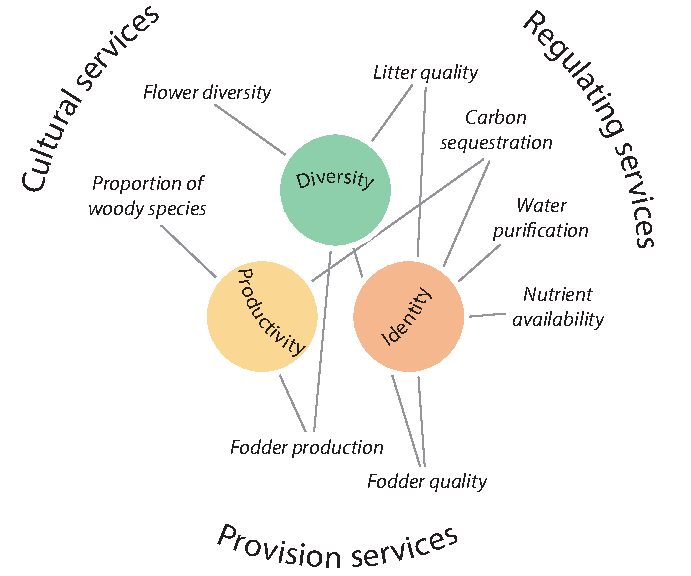
\includegraphics[width=1\linewidth]{./1_Introduction/graphics/services.pdf}
  \caption[Forms of plasticity in models]{Three forms of plasticity in models. }
  \label{fig:services}
\end{figure}

Mountain grasslands provide numerous services, that can be divided into multiple categories such as provision, cultural and regulating services (see figure \ref{fig:services}). Provision services are related to the quantity and quality of primary resources the grasslands provide. Fodder production and quality are the main measures of provision services. Other services can be included in this category: diversity of flowers and phenology for flower production for instance. Productivity is also interesting to assess carbon capture, a regulating service. Soil nutrient availability and water filtering are other regulating services impacted by the identity and diversity of species populating mountain grasslands. Finally, cultural services, related to tourism activity and landscape appeal are also related to grasslands species diversity.


In case of terrestrial ecosystems, vegetation cover is often central because of: it role of primary production, and the fact that vegetation community informs on the properties of the abiotic and biotic conditions. Moreover, a most of studies on services from terrestrial ecosystem are interested in plants and soil invertebrate \cite{de_bello_towards_2010}, revealing the importance of vegetation in the provision of ecosystem services. In addition, in alpine habitats plant communities are susceptible to be the first impacted by the global change because they cannot escape changes in conditions and are the target of management practices linked to fodder productions. All these arguments support the interest of studying the vegetation dynamics for the assessment of ecosystem services.


\paragraph{Properties}
The ecosystem services are tightly related to the \textemph{ecosystem properties} (as illustrated in figures \ref{fig:services})\parencite{lavorel_predicting_2002, diaz_incorporating_2007} that can be extracted from the description of the grassland communities. Ecosystem properties are features of the community that characterise it and arise from the characteristics of all parts of the system or how they combine. The main properties of a plant community are captured in the following concepts:
\begin{itemize}
\item \textemph{identity}: the identity of the community refers to the dominant species (or directly its characteristics) of the community that transfers its traits to the whole community. It can also refer to mean traits (with community-weighted mean measures) of a community. In this document, identity will often be used to talk about the resource use strategy (more or less exploitative). While this notion can encompass multiple traits and measures, it is practical to use one term to identify components of the community description that can be attributed to a species\sidenote{in opposition to variables that are related to a system, \textit{e.g.} diversity cannot be expressed for a species alone};
\item \textemph{diversity}: diversity plays a large role in the provision of multiple services, and is related to other properties of the community. Diversity can be expressed in term of species richness or functional diversity\sidenote{each measure depending on the functional space that is considered}, and by a wide range of indexes that are not discussed here. Despite a lot of nuances between these notions, they are often tightly correlated and diversity will be discussed in term of the number of species or functional volume in the rest of this document.
\item \textemph{productivity}: productivity captures the capacity of the system to produce organic matter in a given timespan. It is an ambiguous term as it can refer to the abiotic environment, to a species or a community property or even to a service. I will try to limit its use to the species or community relative vegetative biomass in a given condition.
\end{itemize}

%-----------------------------------------------------------------------------------------
%\subsection{From community description to ecosystem services: the facets of the community}

%Ecosystem services are various. Some of them can be easily assessed (e.g. fooder production and quality), while others are more subjective (cultural or recreational services) or hard to measure (carbon sequestration, water purification etc...). But all of them rely on a good description of the system, even though this description does not have to be complete as some aspects of an ecosystem might not be relevant to all provided services.


Linking ecosystem services to ecosystem properties is essential both for the understanding of processes controlling these services and for an easier quantification of such services. This is particularly important for the prediction of services levels to plan management practices in the context of global change. Some ecosystem services are here linked to the main community properties as illustrated in figure  \ref{fig:properties}. Because services are hard to assess, ones can take advantage of this link and assess levels of ecosystems services thanks to a detailed description of the community; of both its structure and properties. The structure is defined by the relative abundance of the different species of the community, and properties result from the combination of the structure and the specific characteristics of present species. Multiple drivers affect the relative abundance and characteristics of a given species, from abiotic filtering processes to biotic interactions. So, ecosystem services also largely depend on abiotic factors \parencite{lavorel_predicting_2002}. Therefore, there is a tight link between drivers, community structure and properties, and ecosystem services (see figure \ref{fig:drivers}) that can be exploited to predict changes in ecosystem services \parencite{lamarque_plant_2014}. 


\begin{marginfigure}
    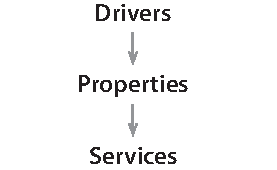
\includegraphics{./1_Introduction/graphics/drivers_properties_services_m.pdf}
  \caption[Drivers to services]{Link between abiotic drivers, community properties and ecosystem services.}
  \label{fig:drivers}
\end{marginfigure}

%The assessment of ecosystem services relies on a detailed characterisation of the community structure and properties. The knowledge of species characteristics and relative abundance allows the computation of summary variables that characterise the plant community. A long history of plant study and description gives us a good knowledge of benefit provided by specific species. 

%

%Need of mechanisms to produce dynamics and give properties.

%\textbf{The complexity of plant community dynamics requires mechanistic approaches to understand and predict system properties in new, extreme, and variable conditions. }


\textbf{The evaluation of ecosystem services relies on a precise description of the ecosystem abiotic and biotic properties. In mountain ecosystems, the plant community is the most dynamic and complex driver of ecosystem services, but direct links can be drawn between the fine description of the community and the ecosystem services. Understanding and prediction the main variables dynamics that capture those links is necessary to efficiently predict changes in ecosystem services levels.}
\textbf{Plant communities are complex interconnected systems. In order to evaluate ecosystem services, they can be summarised by three main types of variables that capture different dimensions of such systems: the diversity, the productivity, and the identity. But grassland communities are natural systems driven by environmental variables, and changes in these drivers can lead  to changes in services because of this link.}



\subsection{Global change: what changes and what consequences}

Mountain grasslands are maintained by strong climatic constraints that limit growth rate and lifeforms  \parencite{koorner_alpine_2003}, but also frequent grazing or cutting perturbation regimes that strongly limit the growth woody species and favour low stature species or rapid growth herbs \parencite{diaz_plant_2007}. But these drivers are changing at alarming rates with negative consequences on levels of ecosystem services \cite{schroter_ecosystem_2005}. Moreover, mountain grasslands are suspected to be very vulnerable \parencite{schroter_ecosystem_2005, engler_21st_2011} due to higher variations in water availability regimes and specific warming processes \parencite{mountain_research_initiative_edw_working_group_elevation-dependent_2015}, stronger isolation (island effect due to rise in temperature) and reduction of the grazing pressure.

\paragraph{Climate change}

The rise of carbon dioxide in the atmosphere due to human activities has a large impact on climate. The constant increase in mean temperature is the most known and easily observable phenomenon (see figure \ref{fig:climate}. But mountain grasslands will also suffer from more frequent and severe drought event, but also precipitation events \parencite{beniston_climate_1997, solomon_climate_2007, intergovernmental_panel_on_climate_change_climate_2014}. They will also experience longer growing seasons and stronger invasive pressure from alien species and species from a lower altitude.


\begin{figure}
    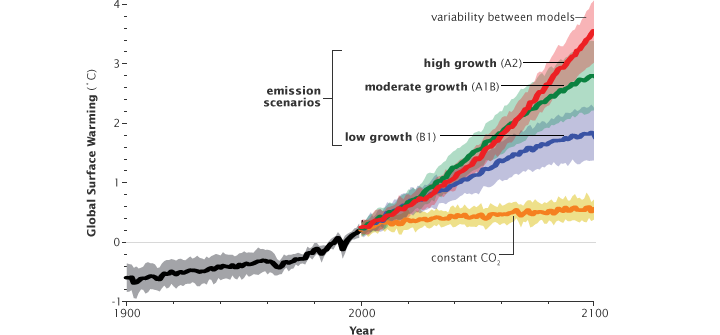
\includegraphics[width=1\linewidth]{./1_Introduction/graphics/ipcc_scenarios.png}
  \caption[IPCC scenarios for global mean temperature]{Historical models and projection scenarios for global mean temperature from \cite{solomon_climate_2007} }
  \label{fig:climate}
\end{figure}

%The changes in snowmelt, season length and drought event will certainly increase the range of conditions alpine plants will experience.
In this context, the aptitude to plants to adapt to such changes and to cope with new competitors, no more filtered out by climatic conditions, will greatly determine the response of alpine communities \parencite{alexander_novel_2015}.

\paragraph{Land-use mutations}

In addition to changes in climate, land use is also modified.  Land-use, mowing or grazing in alpine grasslands, is a great filter for slow-growing perennial species that try to accumulate biomass over multiple seasons. Because of such asymmetric effects, land-use acts as a strong driver and can cause mountain grasslands communities to shift along service gradients \parencite{schirpke_multiple_2012}. Land-use abandonment is suspected to greatly impact the invasion dynamics as it removes the pressure of biomass removal \parencite{carboni_simulating_2017}. 

\textbf{ Global change is a source of considerable changes, both in mean regimes, but also frequency and amplitude of climatic events. In addition to changes in the climatic environment and resource availability, mutation of management of mountain grasslands will also affect community dynamics and particularly competition hierarchy. These modifications of strong drivers will have large effects on plant communities, and therefore their attributes and services they provide.}

\textbf{Mountain grasslands provide numerous services, that can be assessed thanks to the main attributes of the plant community. But global change threats these systems, and as consequence, the ecosystem services we take benefit of. We need tools to anticipate the effects of global change on these services and eventually adapt the management of mountain grasslands.}
%trade-off lavorel and 
%
%management change the position along these trade-offs
%
%climate also change things



 
%
%\section{Community dynamics: complexity emerging from parts and the role of phenotypic plasticity}
%title too vague to bring meaning should put both parts together.
\section{The need for new mechanistic models}


\subsection{The limit of classic patterns}
\paragraph{A new world}

The world is changing at a fast rate \parencite{butchart_global_2010, intergovernmental_panel_on_climate_change_climate_2014}, but most importantly in ways never experienced by living species in recent history. So, anticipating the effects of new environmental conditions on vegetation community cannot be built on the observation of previous or existing states. Extrapolation of complex system behaviour is generally not a good predictor of its actual behaviour. The complexity of the prediction goes beyond the multiplicity of dimensions impacted by the global change (rising mean temperature, frequency, and amplitude of drought events, reduction of cutting frequency or grazing abandonment, etc...), as the drivers often interact, synergise or negate themselves. 

 \paragraph{Find balance}
 
 
 %community responses: different processes (recruitment, growth, plasticity etc...) \& levels (indiv, pop, metacommunity)
 
 To answer this challenge, large-scale experiments are conducted such as Cedar Creek experiment in the United-States, or JENA experiment in Germany. These experiments give high-value experimental data for various conditions and a variety of species, where interactions can be studied as well as management effects. Transplant experiments are also conducted to investigate the effects of temperature rise on the productivity, diversity, and identity of the community (example for SLA response \cite{scheepens_genotypic_2010}, or see \cite{debouk_functional_2015} for an increase in productivity and decrease in diversity, as well as a shift toward more acquisitive species).
 
 But these common garden or transplant experiments also show contrasting response, that can come from opposite responses between intra-specific level and inter-specific level \parencite{jung_intraspecific_2014}, between low and high elevation (changes in identity and contrasting effect in diversity between altitudes, observation data in \cite{rosbakh_elevation_2014}) or between effects (see effect of warming and carbon dioxide on phenology in \cite{reyes-fox_five_2016}).
 
 To accurately predict the future dynamics of grasslands communities, we need to be able to find the balance between dominant effects and eventually identify the interactions. For such complexity, empirical studies provide required and fundamental knowledge of processes and basic differences between effects, but no consensus can be made \parencite{merila_climate_2014} and new approaches need to use.
 
 An additional argument for the use of alternative approaches is the uncertainty around the climatic scenarios (see figure \ref{fig:climate}). Indeed, the future of the planet atmosphere, and by consequence climate, is mainly depending on how we are capable of changing our dependency to fossil energy \parencite{intergovernmental_panel_on_climate_change_climate_2014}. The will to adjust management scenarios to the future of vegetation community \parencite{schipe_multiple_2012} also require extensive experiementation \parencite{rodriguez_lingra-cc:_1999, martin_simulations_2012, deleglise_drought-induced_2015}.
 
 
 
\begin{figure*}
    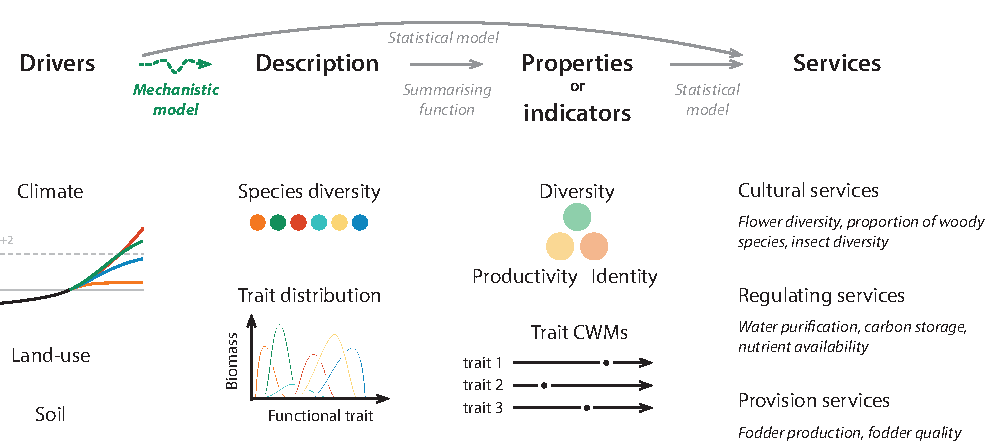
\includegraphics[width=1\linewidth]{./1_Introduction/graphics/drivers_to_services.pdf}
  \caption[From drivers to ecosystem services]{From drivers of community dynamics to ecosystem services. The effects of main drivers (climate and land-use) on grasslands dynamics is capture thanks to mechanistic approaches to predict the composition and structure of the community. This description can then be used to assess the levels of ecosystem services through statistical models, to evaluate climatic scenarios or alternative land-use practices.}
  \label{fig:drivers2services}
\end{figure*}

Mechanistic approaches allow better linking of drivers with community dynamics. This link can then be used to assess the level of ecosystem services as illustrated in figure \ref{fig:drivers2services}.

%niche vs process: stronger effects predicted by niche based because of no plasticity or local adaptation \cite{morin_comparing_2009}



\subsection{When phenotypic plasticity makes things complicated}

Within the context of climate change, the ability of species to adapt has a great influence on the response of the community. Indeed, the capacity of species to adjust to variations in drivers, via genetic variability and mutations, or thanks to plastic mechanisms, will certainly buffer the response of the community to changes in climate or land-use. \cite{morin_comparing_2009} highlight stronger responses to climate change from vegetation communities within niche-based distribution models than within process-based models that capture adaptation mechanisms. More mechanistic processes should be included in these approaches \parencite{evans_toward_2016} to take into account adaptation mechanisms and interactions between species \parencite{gilman_framework_2010}. Plasticity can also change the competition intensity that increases negative effects of climate change  \parencite{hanel_phenotypic_2015}, while it can in other cases shift interactions from competition to facilitation  \cite{callaway_phenotypic_2003}.

Phenotypic plasticity adds another level of complexity to the dynamic of communities and the interacting drivers. Statistical or expert based prediction cannot handle such complexity and mechanistic approaches have great potential to model complex systems.
%The question of adaptation is closely related to intra-specific variations as an intra-specific variation, whether genetic or plastic, are often justified by adaptation mechanisms (selection or adaptive plasticity).


%plus ignored effects of intra-specific variations: additional level of response: amplification or mitigations, driver dependencies?


\subsection{The rise of individual-based approaches}


\textemph{Individual-based-models} (IMBs) let the complex behaviours of systems made of numerous interacting agents emerge from individual functioning. This type of modelling is extremely well adapted to the modelling of plant communities as we have a fairly good understanding of plant functioning and parameters are relatively easy to measure. The dynamics of essential resources is also relatively easy to compute. Yet, this apparent simplicity is relative (to animal modelling for example) and numerous models have been developed with various simplification hypothesis. Most of these hypothesis deal with the essential resources: light in often ignored in grasslands, while forest models focus on this aspect of resource competition. These hypotheses are most of the time justified, and the choice depends on the focus of the modelling exercise, and the importance of the given variables for the dynamics of the system.

\paragraph{Between climate and land-use}
These models are used to investigate the effect of climate change in the study of \cite{rodriguez_lingra-cc:_1999} with the model LINGRA-CC and show an increase in productivity. But the link to land-use practices is always questioned, and in this example, the increase in productivity allows a higher cutting frequency. Alternative scenarios are also explore in other grassland models \cite{taubert_review_2012, taubert_modelling_2014, maire_plasticity_2013, maire_trade-off_2009}. Forest modelling present also numerous implementations of individual-based models (see \cite{ falster_plant:_2016, marechaux_individual-based_2017} for recent forest model examples).

Other models based on processes can be used to study long terms dynamics in the context of climate change in mountain ecosystems. It can be to study patterns of diversity \parencite{boulangeat_fate-hd_2014} or the impact of evolutionary processes on adaptation to climate change \parencite{cotto_dynamic_2017}.
 %an
% to test gc effect on productivity: higher productivity allowing shorter intervals between cutting


%Maire

%Lohier: vegetative phase, coexistence, and ontogeny... 

%Taubert: diversity productivity 


\subsection{Gaps to fill}

A wide range of models has been developed to better understand biological processes involved in plant growth and population dynamics and the impact of climate change and land-use on these dynamics. They spread from organ-based models to functional types approaches. As the scale increases, the resolution diminishes and the verticality of processes is rarely taken into consideration. This is rarely a problem in stable conditions because the lower levels are implicitly integrated into the grain of larger processes (like the leaf gas exchanges regulation processes are ignored at the scale of the population). But two aspects can limit such simplification: (1) if the process is ignored instead of being integrated into higher level function (\textit{e.g.}: stomatal regulation is often not modelled because it is assumed that it is correlated to photosynthetic activity, either because it is limiting the photosynthesis when the vapour pressure deficit is high, or it is down-regulated to avoid water loss when photosynthesis is limited by other factors). However, phenotypic plasticity is often ignored but not translated into the hypothesis of the model. Moreover, variables that are directly impacted by this process are explicitly represented (unlike stomatal conductance with stomatal regulation processes) leading to a misrepresentation of these variables (especially root:shoot ration (RSR) or strategic traits like SLA). (2) if the non-modelled process has a great impact on the dynamic of the system. 

\paragraph{Dichotomy between models}
Among models that target grasslands ecosystems (or more specifically) there is a dichotomy between growth models that are mainly interested in individual processes and species dynamics \cite{soussana_gemini:_2012, taubert_modelling_2014, lohier_analyse_2016}, and models interested in species-level processes and community dynamics \parencite{boulangeat_fate-dh_2014, cotto_dynamic_2017}. The former focus on the individual growth of a limited number of species. They take into account fine-scale resource dynamics and interactions driven by explicit strategies and precise plant functioning. These models are on the side of the spectrum of the development models that often focus on a single species. The productivity of the system is often the primary concern and questions relative to the management of these systems are privileged over questions concerning climate change (but see \cite{rodriguez_lingra-cc:_1999}, but still with the perspective of productivity). The latter is more interested in larger scale dynamics driven by the climate and evolutionary processes. The questions interrogated with these models are therefore more often relative to climate change and adaptive dynamics of the communities and the effects on community diversity and identity. These models are closer to DGVMs despite finer scale interactions. This dichotomy highlight the lack of integrative models that support community dynamics at long time scale with modelling of processes at the individual scale, based on explicit resource dynamics. The explicit modelling of the link between plant strategies, plant functioning, resource dynamics and plant growth allows a solid integration of plant interaction and external drivers (via the effect of resource dynamics and plant growth). Moreover, phenotypic plasticity can be integrated at the plant level, while its complex effects are emergent. Finally, considering the growth of individuals, the strategies of species and the dynamics of the population is required to build predict of all facets of mountain grasslands communities (diversity, productivity, and identity) that can integrate both management practices and climate scenarios.

\paragraph{Where is the diversity}
Because models have often practicality objectives, it is easier to develop a model that can be calibrated with species-specific empirical data. They can also be calibrated with Bayesian procedures and pattern-based approaches \cite{hartig_statistical_2011}. As a consequence, these models often integrate a limited number of species or functional types. This requirement of calibration limits the number of species simulated. To model diverse communities and evolutionary processes, this species diversity is required and generic framework must be adopted to avoid the calibration of individual species. Such diversity is observed in DGVMs that integrate trade-offs and multiple strategic axis \parencite{kleidon_global_20000, pavlick_jena_2013}.

\paragraph{Building bridges}
Mechanistic models are great tools and can be used to explore the uncertain future of mountain grasslands ecosystems. Bridges between individual-centred and generic community dynamics approaches must be built to take into account the complexity of population dynamics emerging from fine-scale interactions and plant functioning, driven both by the environmental conditions and species strategies. Considering both levels is compulsory to capture the complexity of responses of vegetation communities exposed to diverse drivers.

%
%But 2 things:
%(1) ok to not explicitly represent if know and considered within a broader mech (translated into assumptions: \textit{e.g.}: assumption that stomata regulation), it is not the case of phenotypic plasticity as it is not considered in basic assumptions made. Plus, it depends on the scale, but daily growth require plasticity, period.
%(2) they may greatly change plant and community behaviour in changing conditon/environment.
%% 
%scales and processes (climate, management etc...)
%put the resoure in the center (fate-hd)
%
%process and mechanisms
%\parencite{berger_competition_2008}: effect on local env., adaptive beh, below-ground.
%partly filled (maire and Lohier).
%
%but lack of species diversity and genericity. 

%
%
%
%\section{Global change and community dynamics in alpine grasslands}
%\begin{figure*}
%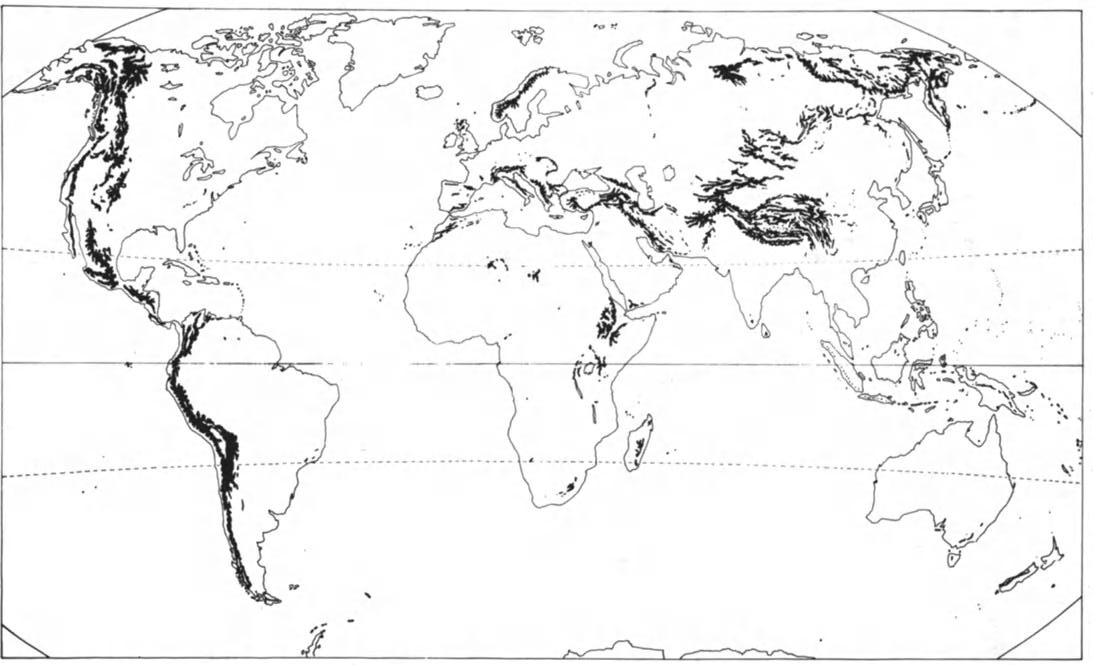
\includegraphics{./1_Introduction/graphics/alpine_distribution.jpeg}
%\caption{Distribution of alpine habitats}
%\end{figure*}
%
%Climate change is probably the greatest challenge the humanity has to face this century. Expected drastic changes in both average climatic conditions and punctual climatic event frequencies and intensities will, and already have, an impact all around the globe on multiple aspects of our lives. From agricultural and economic, to social and political, but also scientific and technical, the problems for human societies are numerous and multidimensional.\\ 
%Need to better understand and predict natural systems. Mountain grasslands are susceptible to be greatly impacted (even if certain think they might not). And in new ways as the rising temperature will certainly lead to migration to higher altitude, increasing the island characteristic of alpine habitats and reducing links between communities, and at the same time increasing the opportunity of invasion by lower altitude higher temperature species.\\
%\indent Detail a bit the characteristic of mountain grasslands, (snow, islands, grazing) the effect on species (snow-bed species, link to meta-community, diversity, species adaptation to frost etc... and how global change may affect that.\\
%\indent Because of that mountain grasslands are rich in species, but also vulnerable, that is why in parallel of predicting climate change, we also need to understand ecological mechanisms under this diversity and how they can be affected by global change \sidenote{section \ref{sec:coexistence}}. A key part in community diversity and in adaptation of communities also lies in the diversity and adaptation of individuals, so we are interested in intra-specific diversity and phenotypic plasticity \sidenote{section\ref{sec:intraspe}}.
%
%
%%Take home message ####################################
%\textbf{There is a need for new tools to predict the response of ecosystems to new climate conditions and management scenarios. These tools should integrate the complexity of such system and the mechanisms underlying the dynamic responses of these communities.}
%
%\section{Empirical results, trait approaches and need for a new kind of model in grasslands}
%
%\subsection{On trait-based approaches}
%
%Holy Graal of ecology\\
%Lavorel, Kraft, Kunstler
%
%\subsection{The importance of intra-specific variability}
%
%Jung
%Leps
%Albert
%Kichenin
%Lavorel (hypothesis of traits bell shape)
%Violle ...
%
%%Take home message ####################################
%\textbf{Trait approaches allow for generalisation and more direct link with processes and services. However they ignore variations and processes at lower levels than the species that are of critical importance for the understanding of community dynamics. A mechanistic approach integrating processes at the individual level and rich community complexity are needed.}
%
%\section{Close a gap in grassland modelling}
%
%%Take home message ####################################
%\textbf{Generalizing models for forest ecosystems and complex individual level models for grasslands coexist, but there is a need for a generalizing model at individual scale for grassland communities.}
%
%\section{Effect of phenotypic plasticity on coexistence and community dynamics}
%
%%Take home message ####################################
%\textbf{Despite empirical and theoretical work, the effects of intra-specific variability and plasticity on community dynamics are not fully disentangled. Understanding the effect of individual variations on plant community is crucial and may greatly alter how we envision the future of these ecosystems.}
%
%%_________________________________________________________________________________
%

\chapter{Aims, Objectives, and Overview}


\section{Aims: understanding and prediction}

Global change is probably the biggest challenge humanity has to face at the beginning of this millennium. Actions are urgently needed to reduce the release of carbon dioxide but also mitigate the effect of climate change on natural and semi-natural systems. While solutions for the former must be found in technology, economics, and sociology, the ecology can help with the latter. But it requires an understanding of how the drivers impacted by global change will impact these ecosystems. The multiplicity of environmental drivers impacted by global change - whose effects can synergise or balance themselves -, in addition to complex structure and dynamics of natural systems make this understanding hard to build and to summarise.

To go beyond traditional pattern-driven ecology and overcome the difficulty of combined causes leading interacting effects, mechanistic approaches should be privileged. 

The functioning of individuals living in these communities and the dynamics of the resources should be at the core of the new approaches to better understand the trajectories of the ecosystems.

%
%Functioning
%Diversity of : drivers, mechanisms, species, and strategies
%Flexibility: structure: genericity, experiments, plasticity

\section{Objectives: a new agent-based model for plant community dynamics} % the why
Traditional empirical approaches of observation and controlled experiments provided valuable information on the functioning of grassland ecosystems. However, they lack the power to understand intricate systems and predict their dynamics, especially in case of uncertain scenarios. 

Modelling approaches must be used to build understanding and predictions of natural ecosystems dynamics driven by changing environmental drivers. These models should include a diversity of drivers as well as the diversity and the intrinsic complexity of these systems.

In order to compensate a long development time and to extend the reach of simulation experiments, models should try to be generic in structure and flexibility at use, while being specialisabled thanks to parameters or simple equation changes.

\subsection{Generic framework for multi-species and plastic plant modelling} % the how

In the context of mountain grasslands, showing unique levels of diversity despite strong environmental drivers, species diversity cannot be ignored to predict the response of the community. This diversity must be translated into species-specific functioning differences leading to diversity in niches and possible responses. In addition to species level dynamics driven by these differences, intra-specific responses cannot be ignored, and a phenotypic plasticity mechanism is needed.



%trade-off that constrain inter and intra differences in the same way

\subsection{Effect of phenotypic plasticity on plant growth, community properties, and dynamics}

Intra-specific variations are expected to play an important role in the response of mountain grassland communities to global change. The effects of phenotypic plasticity and other sources of variations must be disentangled. Explicit integration of species-specific phenotypic plasticity in a plant community model will help identify and understand these effects.

As multiple services derive from the main properties of the vegetation of mountain grasslands, it is crucial to establish how phenotypic plasticity specifically impact these properties. Because these properties depend both on properties of the individuals and the relative abundance and diversity of species, effects on processes at both individual and community scales must be investigated.


\section{Thesis overview}

The rest of this thesis is divided into five chapters. The following chapter \ref{part:literature}, in the form of a literature review, introduces the concepts and knowledge that support the approach developed in later chapters. The chapter \ref{part:model} develops the generic framework for plant functioning and phenotypic plasticity from the concepts established in chapter \ref{part:literature} and further extended. Chapters \ref{part:individuals} and \ref{part:community} present respectively individual and community scale results of simulations made with the developed model \model on the effects of phenotypic plasticity on main plant community properties. Finally, the final chapter discusses the outcomes of this work and possible paths to follow from the presented conclusions. Extensions to develop on the model are also proposed.


\begin{figure*}
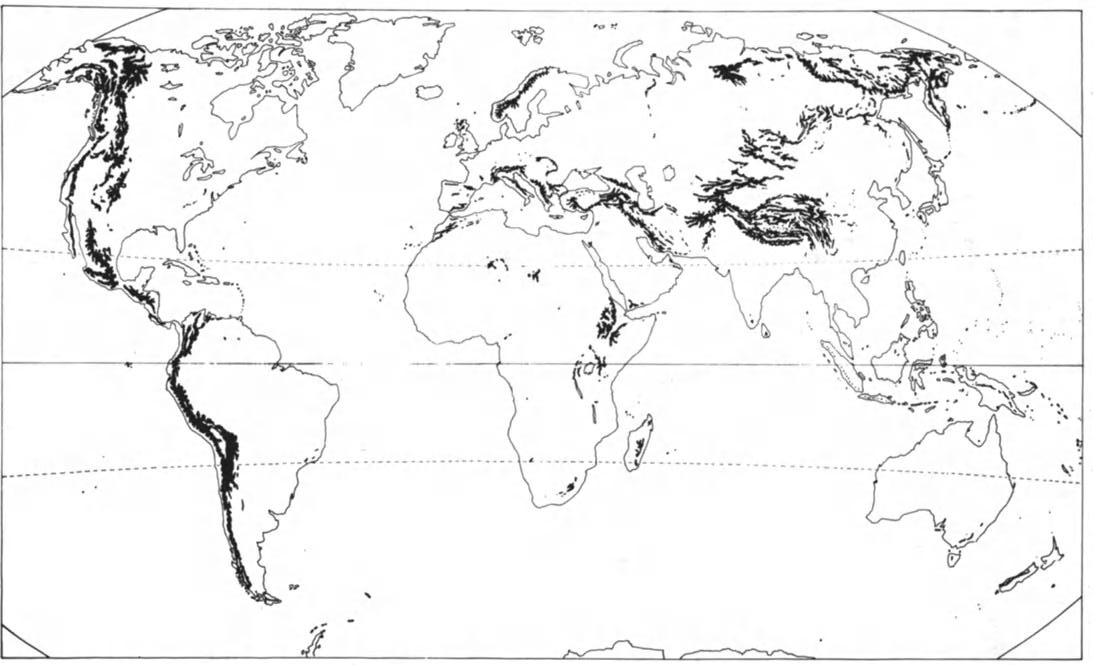
\includegraphics{./1_Introduction/graphics/alpine_distribution.jpeg}
\caption{Distribution of alpine habitats. Alpine habitats shelter unique and rich ecosystems providing numerous services to human populations. Climate change and mutations of land-use practices threaten these dispersed and fragile habitats. From \cite{korner_alpine_2003}.} \label{fig:distribution}
\end{figure*}

%\includeonly{./1_Introduction/Introduction}
%%\addbibresource{../../Bibliography/bib_zotero20171106}

%\chapter{Mechanistic model for plant community dynamics centred around carbon allocation}
%Paper 1:
%\section{Introduction}

\begin{fullwidth}
The objective of this chapter is to develop the core concepts of the model, introduced in the previous chapter, and to explain the structure and design choices made during the model development. The first part focuses on the general context of alpine grasslands and some coexistence mechanisms at stake. The following part details the definition of the strategy space and the modelling of phenotypic plasticity while introducing the key concepts of species memory and individual experience. Finally, the last part is a detailed description of the model following \parencite{grimm_standard_2006} recommendations.
\end{fullwidth}

\chapter{Alpine environment: conditions, resources, and perturbations}
\section{The scales of alpine grasslands}

\paragraph{The scale}
The \textemph{scale} is a determinant variable in the quantification of mechanisms that structure ecological communities \parencite{bello_hierarchical_2013}, and therefore in modelling approaches. It is chosen based on structures that the modeller intends to explore and determine the upper limit of mechanisms the model can reproduce. Large scales will favour geo-climatic and dispersal effects \parencite{kleidon_global_2000} while small scales will focus on direct plant interactions processes or resource heterogeneity \parencite{ soussana_gemini:_2012, maire_plasticity_2013, taubert_modelling_2014}. This is true for spatial scale, but also temporal scales. Because mechanisms studies at large scales like dispersion, invasion, speciation occur over long time scales whereas mechanisms occurring at smaller spatial scale, like competition, facilitation, disturbances play a role on shorter time scales, spatial and temporal scales are often correlated. The scales are also dependent on the studied environment. There is a high contrast between highly productive environments like tropical forests and unproductive environments like mountain grasslands. The dimensions of individuals themselves are a constraint on the scales: while tropical trees grow few tens of meter high and above one meter diameter, alpine grasses do not exceed half a meter \parencite{korner_alpine_2003}. Similar differences in the order of magnitude can be observed for life cycles between long live tree and annuals or bi-annuals grasses. The focus of this work being on plant functioning and interaction mechanisms, the scale of the model will be around the meter, while the temporal scale will be in the order of the season.

\paragraph{The resolution} The same way the scales are constraint by the size or length of the individual, the \textemph{resolution} should be close to the size of the modelled entities. The resolution is also determined by the focus of the model: interactions between individuals must be distinct and not blended to hope see the emergence of spatial patterns. Cell size and time step length should be small enough to take into account heterogeneity that is an important driver of diversity. For these reasons, the spatial resolution is set up to the centimetre and the temporal resolution to the day (can be changed but processes might not scale well).

\paragraph{Complexity and performance}
Once the resolution is fixed there is always the temptation to increase the size, or scale, of the system. This should be avoided for two main reasons. (1) the increase of scale with relatively fine resolution lead to a high increase in computational power required for simulations that are already complex. (2) there is a high chance that the processes modelled at fine resolution lose their sense when scale increases. Indeed, as mentioned, the importance of processes at stake is often dependant on the scale the system is studied. The effect of higher scale processes is often taken into account in inputs or parameters. Calibration of these parameters against certain data is a way to better understand these processes \parencite{lagarrigues_approximate_2015}. 

\section{Resources: light and water}
As mentioned in the previous chapter, resource fluctuations, heterogeneity, and competition are important factors for coexistence. Unlike animals, plants mainly compete for the same resources: light, water and nutrients. Light is the source of energy that allows the transformation of inorganic carbon into organic matter through photosynthesis. Water has multiple functions in plants: transport, structural support, and oxygen supply for photosynthesis. Nutrients are used in the construction of cells and cell walls, and especially the production of proteins that act as cell machinery.

\section{Perturbations: frost, grazing, and mowing}
\paragraph{Climate}
The most notable specificity of mountain grasslands is the climate. While there is a wide range of mountain grasslands type, the focus of this document is in French Alps. The alpine climate in France is characterised by cold winter with snow precipitations and dry summer. The growing season is relatively short and spread between May and October in low altitude, and June and September in high altitude \parencite{korner_alpine_2003}. The particularity of this habitat is the presence of snow cover during winter that protects soil, rhizomes, and seeds from negative temperatures. Because of this, seasons are decomposed in the model based on the snow melt in spring/summer and the first snowfall in winter. While a rise in temperature is needed to allow snow to melt down, frost event can occur after the beginning of the season. Such events represent strong environmental filter for non-adaptive plants that do not invest in specific resistance mechanisms to favour early germination and growth. Therefore there is a strategic trade-off between germination date and early growth with frost resistance.

\paragraph{Management}
Another specificity of alpine grasslands is that they are subject to changing management practices. Mountain grazing by domestic cattle was fairly common in the Alps, but changes in agricultural practices and a decrease in productivity due to drought lead to less and less grazing or mowing for fodder in alpine grasslands. These two types of management have different impacts on the community. While mowing is non-specific and favours small plants, herbivory is known to be specific when the production is greater than the grazing pressure. Leaves with high nutrient content and low structural tissues content are generally favoured because of high input and high digestibility. The grazing pressure plays as equalizing mechanisms as it favours conservative species with lower competitive ability.

Other forms of herbivory can happen in grassland context, but the extent of the grazing by large herbivores reduce the relative importance of this effect and allows us to ignore this diversity of herbivory sources with complex dynamics.


\chapter{Multi-dimensional strategy space, carbon pools, and trade-offs} \label{chapter:strategy-space}
\section{Multi-dimensional strategy space and allocation pools}
%Leaf economic spectrum + Shipley + Poorter
%
%\subsection{Allocation or anatomy: a choice to make}
%what is SLA and SRL: cost of exchange area: tissue density, tissue thickness. Poorter 2009, grace2017, Katabuchi 2017, de la Riva 2016\\
%THere is not only coordination -> part of RSR is explained by SRL:SLA\parencite{freschet_explaining_2015}. Multiple sources of information (memory) that affects these traits: composite traits that affect multiple fitness dimension -> memory not only for the climate. -> but also coordination. A more tight trade-off for root with smaller changes in SRL and more changes in RMF, the opposite for SLA. Need for a model that allows such asymmetry. 
%\parencite{freschet_integrated_2015}
%\\
%within species LES %hu_novel_2015

\subsection{The strategy space in \model}

\paragraph{What is a strategy space}
In an ecological agent-based simulation model a species will be defined by its values for the species-specific parameters. They can be estimated from experimental data \parencite{taubert_modelling_2014, maire_traits_2009,lohier_explaining_2014} or be picked from a strategy axis \parencite{reineking_environmental_2006, kleidon_global_2000} composing a strategy space \parencite{westoby_leaf-height-seed_1998}. The diversity of the species pool will depend on the number of values for each of these specific parameters, or traits, and the number of these traits. Each trait increasing the dimension of the strategy space \parencite{laughlin_intrinsic_2014}. The ambition of this model is to simulated rich plant communities, the definition of these axes is crucial. Trade-offs between traits are excellent applicants for these specific parameters as they reduce the dimensionality of phenotypes to a small number of dimensions \parencite{wright_worldwide_2004, diaz_global_2016, reich_world-wide_2014} while keeping the information of traits needed to describe the plant functioning. Trade-offs emerge from ecological and physical or biological constraints, by considering these constraints Darwinian demons are avoided.\\

While considering too many axes does not improve community description, a certain number is needed to have strategic diversity \parencite{laughlin_intrinsic_2014}. This is intuitively explained by the fact that each trade-off is closely related to a particular aspect of fitness or mechanism for coexistence (\textit{e.g.} reproduction, competitive ability, resistance to resource shortage, predation, etc.). In this model, multiple aspects of plant life are represented: germination with the germination rate for storage effect \parencite{chesson_general_2000, adler_climate_2006}, dispersion with seed mass \parencite{westoby_leaf-height-seed_1998} or tissue construction cost \parencite{reich_leaf_1992, wright_worldwide_2004, reich_world-wide_2014}. Main components of plant growth and life history are covered by such trade-offs and driven by mechanisms shared by all vegetation systems. Because of that, the model has a great potential of genericity and diversity. It can be easily adapted to other plant communities with specific calibration, and extended to couples of biological process and differentiation axis (\textit{e.g.} root herbivory and associated resistance carbon pool). The the trade-offs used in the model are detailed in the model description below \sidenote{see section \ref{chapter:model-description}.}. These axes should, in such models, be independent, (\textit{i.e.} it is physically and biologically possible for a plant to take any position in the space drawn by two given axis) and result from physical or biological laws (ensuring that impossible strategies are indeed excluded from the model). First, it is a condition for parsimony of the model. The second and more interesting reason is that any trade-off emerging from the model should have an ecological interpretation \parencite{maire_disentangling_2013}. \\
 

One way of constraining plant strategies to certain axes is to consider allocation trade-offs \parencite{kleidon_global_2000, reineking_environmental_2006}. An allocation trade-off is the translation of the mass conservation rule that prevents the allocation of biomass to distinct carbon pools. If biological functions are related to organic matter pools (photosynthesis to leaves, water and nutrient uptake to roots), then the sum of biomass to invest in each carbon pool (therefore in each function) cannot exceed the total available biomass: leaving the plant with a choice on the balance between the different functions. Allocation trade-offs have the advantage to be easily implemented and be intuitive. By design, a partitioning factor value corresponds to a position on the related strategic axis. In \model, 5 main trade-offs are captured by allocation trade-off: (1) development vs reproduction: partitioning factor between reproduction and maintenance of vegetative tissues (when plant is mature), (2)  persistence vs dispersion: partitioning of reproduction biomass between persistence (storage) and production of new propagules (seed/clone production), (3) aboveground vs belowground competition: investment between shoot and root, \parencite{kleidon_global_2000, reineking_environmental_2006, taubert_modelling_2014}(4) slow vs fast: construction cost trade-offs between active and structural tissues in both shoot and root and (5) growth vs resistance: partitioning between stored biomass and frost resistance carbohydrates \parencite{cai_changes_2004}. This last trade-off can be extended to other carbon pools of specific resistances, for example to herbivory. Modification of these coefficients during life history is a way to introduce plasticity in the model. The rules driving such changes for some of this partitioning parameters are described in the following section.\\


One of these trade-offs, (4) slow vs fast, is key and related to the construction cost of organs (independently leaves and roots). Highlighted at the global scale and for leaves, the Leaf Economic Spectrum \parencite{wright_worldwide_2004} draws a strategic differentiation axis from conservative slow species and exploitive fast species. The construction cost has long been identified as a factor of strategic differentiation in plant communities\parencite{westoby_leaf-height-seed_1998}. This strategic axis, being related to many functional traits: SLA, LDMC, LNC, leaf longevity, Amass, etc.\parencite{wright_worldwide_2004} is of crucial importance. First, these traits are closely related to the characterisation of plant communities and the assessment of services \parencite{grime_benefits_1998}. Second strong links and correlations can be made between these soft traits physiological traits \parencite{craine_functional_2002, reich_variation_2003, wright_worldwide_2004}. Finally, a species resource use strategy is closely related to its responses and vulnerability to changing conditions \parencite{poorter_causes_2009, dwyer_specific_2014, deleglise_drought-induced_2015}. The traits related to this trade-off play a major role both in individual growth and physiology and in community services and response to a gradient. Therefore it is essential to the model. Analysing the underlying mechanisms for such strong trade-off is necessary to implement satisfying representation in the model.\\

%\textbf{Change this: maybe start with Shipley results, then composite stuff. Question: should it be here, or in the following part ?}

These trade-offs between highly productive tissues with low construction cost and short lifespan called exploitative, and more conservative strategy with longer lifespan but lower productivity are mainly observed thanks to soft traits such as SLA for LNC \parencite{wright_worldwide_2004}. Mechanistic models require traits related to physiology and organ performance \parencite{soussana_gemini:_2012, lohier_explaining_2014}, but a link can generally be done between these traits and soft traits. However, traits such as SRL or SLA are composite traits emerging from different organ properties \parencite{ryser_importance_1996,john_anatomical_2017}, where tissue density and organ thickness are the main determinants. "\textit{A necessary trade-off between allocation to structural tissues versus liquid phase processes}" has been identified by Shipley et al. \parencite{shipley_fundamental_2006} as one of the two main factors for the leaf economic spectrum to emerge. Such allocation trade-off can indeed explain differences in construction cost as the liquid phase corresponding to the "active" part of plant tissue, the cell content, have much lower dry volumetric mass than its "structural" counterpart, the cell-wall. Also, active tissues containing the protein machinery for photosynthesis and water absorption, a higher proportion of high protein concentration tissue would be correlated to higher nitrogen concentration in the organ on the "fast-slow" spectrum, along with a higher mass-based photosynthetic rate \parencite{reich_world-wide_2014}. On the other end, the structural tissues give the organ a higher lifespan \parencite{mediavilla_internal_2001, ryser_importance_1996} that compensate for lower productivity \parencite{westoby_time_2000}. Such trade-off can be apply to both shoot and roots \parencite{craine_functional_2002,  tjoelker_linking_2005, reich_world-wide_2014}. From that, the decomposition of organs between active and structural tissues constitutes a strong basis to model construction cost trade-offs as the main parts of the global strategy space.\\

A similar axis of differentiation has been demonstrated for roots \parencite{reich_world-wide_2014, tjoelker_linking_2005, picon-cochard_effect_2012}. The necessity for independent similar axis for leaves and root can be discussed with respect to coordination between shoot and root activities. Because perfect equilibrium cannot be guaranteed in all conditions, strict coordination cannot be taken as a principle for the reduction of strategy space. Moreover, empirical results suggest small deviations from coordination are common \parencite{freschet_explaining_2015}. The leaf economic spectrum being conserved at the intra-specific level \parencite{ hu_novel_2015} is another reason to include such trade-off as it would be a good basis for phenotypic plasticity \parencite{freschet_plasticity_2013}.\\


%Take home message ####################################
\textbf{The use of allocation trade-offs allows the construction of a generic multi-dimensional strategy space where a high diversity of species can potentially coexist. Because this space is based on physical laws, it ensures the non-existence of Darwinian demons and does not limit the species or individual plants to tested parameters and strategies. To be complete, the link between carbon pool allocation and physiology must be defined, respecting similar biological or physical laws.}

\section{Craft a trade-off: active and structural tissues}

Allocation trade-offs offer great flexibility and are easily understood and implemented. However, when they control the value of traits (SLA or SRL) involved in multiple processes, a balance must be found to avoid that: (1) one process is ignored because it has a low relative importance for fitness (becoming useless to the model), (2) the effects of processes involved show strong response curves to the allocation and there is only one global\sidenote{I use the term global here to designate the multidimensional space draw by the axis of interest and other variables play a role in involved process (e.g. resource availability, temperature etc...).} optimum. The idea behind a trade-off is that multiple positions are viable in different conditions or in association with other strategies. The leaf-economic spectrum, in addition to relying on the active-structural tissue trade-off, also requires "\textit{an evolutionary trade-off between leaf photosynthetic rates, construction costs, and leaf longevity}"\parencite{shipley_fundamental_2006}. This trade-off is explored in this section of the document.\\

In the framework of the model, plants share the same global parameters, as it should also be the case for photosynthesis parameters. Because photosynthesis relies on the exchange of gases ($CO_2$, $O_2$ and $H_2O$) and the interception of light, it is related to exchange area. Considering one shared parameter for maximum area-based potential exchange rate satisfies both the need for a shared parameter and a way for plants to varying their mass based exchange rate by changing their proportion of active tissues. This is in agreement with the LES that a strong relationship between mass-based traits and limited ones for area-based variables \parencite{wright_worldwide_2004}, and explain the first part of the trade-off between photosynthetic rate and construction cost. The second part is the relationship with the longevity. The longevity is often correlated to SLA in empirical studies, however, this is mainly explained by differences in tissue density and toughness than in thickness (another component of SLA). For this reason, we can directly link the leaf longevity to active tissue proportion. Respiration is also increased by the increase in the proportion of photosynthetic tissues \parencite{kleidon_global_2000, reich_world-wide_2014}. We have now a trade-off between a gain function (exchange area gain by changes in densities) and a cost function (tissue turn over and respiration). This should be enough to explain different strategies \parencite{westoby_leaf-height-seed_1998}. However, the model needs internal limits to avoid the gain function to lead to only active tissue organ (or only structural). These limits are required to allow individuals or species to change position along these axes (plasticity or strategic shift). The convex shape of gain function in association with a minimal cost (minimum turn-over cost above maximum potential gain) is enough to limit the allocation to structural tissues only. To avoid allocation to only active tissue, that would correspond to an organ made of protoplasts, the cost function needs higher than the potential gain. To achieve that an exponential function is chosen. This choice ensures that the potential gain function has an optimum different from the borders.\\


The tissue density is only one of the dimension of the SLA, and plants also vary their thickness in response to resource gradients \parencite{poorter_causes_2009}. For simplicity reason, only the density dimension will be considered in the model, while others tend to prefer only the thickness \parencite{feller_mathematical_2015}.



\paragraph{Gain as a function of conditions}

To allow diversity to emerge from temporal and spatial resource heterogeneity, the potential gain (productivity) of plants must be a function of both the plant strategy and the external conditions. While it makes no sense to have the productivity independent from the external conditions, if it is only driven by those, then the model is either a neutral model and the plasticity makes no sense in such model, or a model where only one strategy is the best, and plasticity would just allow the convergence toward this unique optimum phenotype. There must be different strategies dominating different habitats. 

This requirement is taken into account in the construction of the trade-off between the active and the structural tissues. The costs are mostly controlled by this allocation trade-off. The potential gain is not only a function of active tissue proportion but also depends on resource availability. Changes in resource level imply changes in the slope of gain function and a shift of the organ optimum for tissue allocation. This shift makes more conservative strategies more interesting when resources are scarce, while more exploitative allocation strategies are better for high resource availability. This link between optimum allocation and resource level could be used to define the best phenotype according to experience conditions, but the organ strategy cannot be disconnected from the whole plant strategy and allocation. %While there might be a function that links all possible resource availability combination (authorising plant life) with the best corresponding phenotypes, this function is not easy to compute because the whole plant scale must be considered\sidenote{the mutual dependence between the two organs makes the problem non obvious.} and such optimum may not correspond to an optimum in a more dynamic system.\\

The phenotype (within the subspace of vegetative allocation) depends both on the individual efficiency of organs and the balance between shoot and root activity. This balance often used to model plant plastic allocation and considered between light and nitrogen \parencite{soussana_gemini:_2012, lohier_explaining_2014}. In the context of mountain grasslands and global change, the water is more important and will certainly be more variable. The integration of nitrogen as a limiting solution would allow more functional diversity but complicates the optimisation problem that is the plasticity. 

% There you have to sell your memory stuff!

\subsection{Species memory and phenotype determination}\label{subsection:memory}


\paragraph{Vegetative phenotype axis}

As mentioned, the overall plant productivity is a function of three main \textemph{phenotypic axis}: the root mass fraction (RMF), the proportion of active tissues in roots (PAR], and the proportion of active tissues in the shoot (PAS). These three dimensions define a vegetative phenotypic space. The phenotypic plasticity consists of rules that drive the trajectories of the individual plants within this space to improve their performance relative to a fixed position. Modellers have to find a way to link the species-specific strategy with this starting point and the trajectories the plant can follow. This link is given by the concept of species memory of the species that translate the genetic information of the species in an information that have sense and can be manipulated.


\paragraph{Memory of species: a driving trait}

 In a non plastic context, the strategy and the phenotype are one thing, and there is no need (from the plant perspective) to associate this phenotype with the external conditions. In a plastic context, the phenotype, in addition to being linked to the overall plant strategy, is also linked to the external conditions (by the plasticity rules). There is a dependency between the plant strategy, its phenotype and the external conditions. In one direction, the conditions define an optimum phenotype (or phenotypic subspace) that best fits them. In the other direction, a phenotype corresponds to a set of favourable conditions and therefore contains these climatic conditions. This can be seen as the species \textemph{memory} of the conditions captured by mutation and selection processes. When the plant starts growing, it has no prior information on the external conditions yet but expresses a species-specific phenotype by default \sidenote{in a non plastic context, this phenotype is maintained over time.}. Because of the link between this phenotype and the external conditions, this starting phenotype can be expressed as a function of species strategy and expected conditions. The genetic information that defines the starting phenotype is partially expressed by the memory of the species and its strategy traits. It could be that the memory is enough to define the starting phenotype is there is an explicit function that links a set of conditions with an optimum phenotype. While this makes the concept of memory neater, it reduces a lot the possibility of diversity and supposes that evolutionary processes would have selected the best phenotype rather than the phenotypes that are able to maintain themselves. In \model, this partial constraint, defining a subspace rather than an optimum phenotype is illustrated by the control of the root mass fraction (RMF). The balance between the shoot and root activities being key in the overall plant performance, the RMF will be determined as a function of the species memory. The other strategy traits are defined independently and characterise the strategy of the species.
 
Because the phenotype is defined from this memory, the plasticity can then be imagined as a modification of the information given by the memory based on the experienced conditions. The plasticity is then a balance between this prior information contained in the species genetic information - the \textemph{memory} - and further information given by the conditions lived by the plant - the \textemph{experience} - leading to a posterior image of the conditions - the \textemph{estimation} - driving the trajectory of the plant within the phenotypic space.
 
 
 The concept of memory, in addition to link the starting phenotype/strategy with the plant trajectory/plasticity, also opens the door to the modelling of heritability by a meaningful alteration of this memory. If the experience of a plant does not match its species memory, it could change this value to transmit this information to new propagules.

%
%phenotype = ensemble of response trait values. Emerge from default trait + environment.\\
%Composite traits are defined by the interaction of different, independent, driving traits. What is a driving trait? Biology: genetic information. This genetic information is selected by climatic conditions. If we can make a link between optimum value for a trait and environmental conditions, then store external conditions and use the link between.\\

%

%Th example of the leaf trade-off and the importance of resource availability for optimum position.\\


%The coordination and the difficulty to define a phenotype\\


%Take home message ####################################
\textbf{The decomposition of organs organic matter in active and structural carbon pools makes a link between allocation and physiology and draws a subspace within the strategy space where individuals can move and change their phenotype. Limiting mechanisms restraint the viable options to realistic values along these axes. Within this space, the resource availability and external conditions play a major role in the expression of the strategy. The memory of the species offers a starting point for the phenotypic trajectories of plants driven by the plasticity rules that have to be defined.\\ %not convinced by this last part.
}


%Chapter take home message ####################################
\textbf{The identification of axes of strategic differentiation enables the definition of a strategy space for the modelling of species rich communities. The main resource-use strategies within this strategy space rely on established allocation trade-offs. Because they link physiological parameters with carbon pool sizes, these trade-offs allow to model contrasted plant behaviour in a realistic way. The effect of changes on allocation strategies on physiological processes can also be modelled thanks to this explicit link.}

\chapter{Modelling phenotypic plasticity}\label{chapter:modelling_PP}


\section{Plasticity as a strategy: between species memory and individual experience}

\subsection{A concept of active plasticity as a strategy}
\paragraph{The decomposition of plastic response}
The active plastic response is highly integrated \parencite{freschet_integrated_2015} and involve a lot of regulatory processes\parencite{nicotra_adaptive_2010}. It is impossible to represent all regulatory processes involved in an APR (because of our lack of knowledge and their complexity). Alternatively, the concept of \textit{integrated response} can be conceptualised. It supposes a link, or coordination, between the experienced conditions and the phenotypic response. This can be translated, in the model framework, by the existence of an explicit link between a representation of external conditions and a phenotype matching this conditions: the \textemph{allocation rule}\sidenote{the use of the word \textit{allocation} is justified here since the phenotypic plasticity in \model is reduced to changes in allocation.}. Another key work is \textit{anticipatory}. It supposes that the plant knows, or at least have an idea of the future conditions. This is really the point of an active plastic response: change the phenotype to better match future conditions. A representation of future is also called a \textemph{projection}. The projection and the allocation rule together form the active plastic response.\\
If allocation rule is not obvious and is discussed later(see paragraph \ref{section:allocation-rule}), the idea of projection is fairly intuitive. The projection will correspond to a value for a given metric that represents the external conditions. It can be resource availability level, temperature, herbivory risk, etc... If such metrics can be given at the community scale, it makes sense to use a plant-centred measure of these variables for two reasons: (1) take into account the spatial heterogeneity, (2) plant experience of conditions is necessarily egocentric. The details on how experienced conditions are interpreted by plants in \model are described in section \ref{chapter:model-description}.

\paragraph{Control of plasticity}
Active plasticity is now represented by a projection and an allocation rule. However, how a species can control the whole process is unclear. In theory, both projection and allocation rule can be species-specific. In nature, plants generally have structurally similar regulatory processes\sidenote{see box in section \ref{part:literature} \ref{chapter:PP_ISV}.} and responses to external stimuli are translated (and stored temporarily) thanks to the accumulation of chemical compounds. These mechanisms suggest that, while the allocation rules are mainly shared, individuals vary on the information level (i.e. the concentration of phytohormones), or in the context of the model: plant vary in projection. This control of active plasticity is supported by the model design. The number of rules that can drive the allocation is reduced and discrete, while the projection is multi-dimensional (one dimension per external variable considered), continuous and highly flexible with a reduced number of parameters\sidenote{details in paragraph \textit{estimation of conditions} in section \ref{chapter:model-description}.}.
For this reason, \textemph{projection} is chosen to be the \textemph{controlling factor} of active plasticity, while the allocation rule is fixed and shared between all species. Therefore an individual with fixed projection won't be actively plastic, despite the fact that it could express apparent plasticity because of external factors: reduced resource availability, grazing, frost damage, etc... The model has now a concept for active plastic response\sidenote{In the rest of the document terms \textit{plasticity} or \textit{phenotypic plasticity} will refer to an \textit{active plastic response}.} controlled by the projection of external condition. The next question that needs to be answered is: how do species differ in their plastic response ?\\

\subsection{Species specific plasticity: the balance between the species memory and the individual experience}

\paragraph{Species specific plasticity}

In \model, the projection of external conditions is the means for plants to alter their phenotype in response to changes in experienced conditions. Since the allocation (or driving) rule is shared by all plants, if the projection of external conditions is also shared by all plants, then is the response still active plasticity? The first intuitive answer is \textit{yes} since the conceptual framework is respected and plants would react to changes in conditions that would affect the projection. But, such response would be equivalent to a direct external control of the climate on the phenotype. In such case, species would not have control over how the phenotype varies, that would be fully controlled by shared projection and shared allocation rule. This is passive plasticity. To have proper active plasticity, the species need to be able to \textemph{regulate} the plastic response. If species can regulate plastic response thanks to species-specific parameters, plasticity becomes a \textemph{strategy}. This is in agreement with Bradshaw's vision of phenotypic plasticity as a trait, or a character, subject to selection and evolutionary processes\parencite{bradshaw_evolutionary_1965, bradshaw_unravelling_2006}. How do species regulate the plastic response to make it a strategy?\\

Therefore, to have a proper \textemph{strategic plasticity}, the plants need to control the plastic response, so in \model to control the projection. This modification of the projection makes the specificity of the plastic response and allows diversity in plasticity. 
%\textbf{Plasticity}: expected environment -> phenotype, here phenotype is equivalent to biomass partitioning, that means expected environment -> allocation coefficients. Then memory -> expectations -> allocation. Because low dimensions, and we want diversity, and the link between memory and allocation might not be a function (one memory give exactly one optimum allocation), in the model this relationship is not verified. Species-specific traits are used to allow for different strategies to be associated with the same memory (different plants won't have the same strat, despite sharing the projection)\\
%Once the plasticity is introduced, talk about the memory. Now you can also talk about the mapping/consistency between both and the difficulties to use both.



%\paragraph{Build a projection}
\paragraph{Species memory and individual experience}
The projection is the way plants control phenotypic plasticity. A projection is an idea of the future based on available information and on the understanding of a phenomenon. Ones could discuss what is the understanding of the climate by plants, while others can focus on how to represent such understanding and state that fine molecular regulatory processes can reproduce and store such information. The focus is on the construction of the projection with respect to the different sources of information a plant has: (1) its experience of climate and external factors, and (2) its ancestors' memory\sidenote{see paragraph \ref{subsection:memory}.}.\\
While, for any given individual plant, the experience of external conditions varies in time, the memory stays fixed. There is a clear contrast between the variable experience of conditions and the fixed species memory. A way to represent different strategies and the level of control the plant apply on projection is to vary, between species, the relative weight of species memory against individual perception. This species-specific parameter, the \textemph{confidence in species memory}, sets the \textemph{stability} of the projection with respect to individual experience. The capacity to adapt the phenotype to changing conditions is directly linked to the projection changes. High confidence in species memory translates in a low amplitude of projection variations, and though in low active plasticity.\\
The calculation of projected resource availability levels, or temperatures, are detailed in the dedicated paragraph of the model description. The key message is that the species has control on plasticity with both its confidence in species memory and the said memory that alters the projection. %The relative impact of memory and confidence is described in figure \ref{fig:memory-confidence}.

% The species-specific memory of external condition has been described\sidenote{paragraph \ref{subsection:memory}} as a way to match certain traits (mainly root:shoot ratio) with external conditions. The memory is a metric of resource availability that is used to partly (potentially entirely) determine the phenotype of plants.


\section{Driving rules of allocation}\label{section:allocation-rule}

\textemph{Allocation rules} are determinant in the model behaviour as it is shared by all species, and link the projection of conditions with the phenotype. The objective of the allocation is to define the target phenotype for a given individual while considering the information about the external environment and the state of the individual. It has been established that the current model will rely on a projection of the conditions to establish such target phenotype. Therefore, the allocation rule characterises the mathematical link between this projection, the current state of the individual and the target phenotypes. The definition of the target phenotype resides in the solving of the system defined by the allocation rule, the projection and the individual state. Depending on the allocation rule, the system can be strongly constrained by the allocation rule, reducing the number of solution, but also leading to strong convergence between individuals sharing the same projection, and difficulties to model diverse communities. Alternatively, a less constrained link between the projection and potential target phenotype would define a sub-space solution rather than an unique solution. An addition rule is then required to define the target phenotype. This additional rula can be function of the individual state (\textit{i.e.} phenotypic distance) reducing the convergence between individuals and allowing more diverse communities. While the allocation rules can have strong effects on the plastic behaviour of modelled plants, the main objective of these rules should be to improve fitness. Comparison to empirical pattern should allow us to test the validity of such rules.

%\textemph{Allocation rules} are determinant in the model behaviour as it is shared by all species, and link the projection of conditions with the phenotype. Multiple options are possible to drive plasticity, but they can be divided into two main categories: (1) determining, (2) directive. Function from the first category defines an optimum phenotype (within the plastic strategy space), while functions from the latter group defines an optimum sub-space and other criteria (than the  are needed to determine the exact new phenotype.\\
%The two type of rules have different strengths and weaknesses that are detailed in table \ref{table:allocation_rules}

%\begin{table}
%\caption{Two types of allocation rules: strengths and weaknesses} 
%\label{table:allocation_rules}
%\begin{center}%
%\begin{tabular}{l c r}
%Strength or weakness & Determining & Directive \\ 
%\hline 
%Phenotype fully determined & \textcolor{myGreen}{$\bullet$} & $\circ$ \\
%Risk of convergence & $\bullet$ &  $\circ$ \\
%Reduction of functional diversity & $\bullet$ &  $\circ$\\
%Discrepancy between parameters & $\bullet$ &  $\circ$\\
%Strong plasticity effect & \textcolor{myGreen}{$\bullet$} & $\circ$
%\end{tabular} 
%\end{center}
%\vspace*{0.5cm}
%\end{table}


One of the assumptions of the plasticity developed in this document is the existence of a tight relationship between experienced condition and fitness. A subsidiary assumption in the implementation of this plasticity is that this function can be captured, or modelled, by the same functions that drive plant growth. In other words, simulating individual growth, using the estimated/projected conditions as parameters, day by day, is enough to capture the link between environmental conditions (experienced by the focal plant) and plant growth\sidenote{that takes here the value of fitness proxy}. 

A determining allocation rule would try to explicit this link function and optimise it. In other words, find the phenotype that maximises the gain function. While evolutionary processes allow the integration over time of the effects of phenotypic changes, it is not possible to consider this dimension without a long-term projection of the conditions. So the temporal dimension is excluded, and the maximisation of the daily gain is hypothesised to maximise the gain over time. On the other hand, a directive function would identify a subset of acceptable phenotypes. Then, an additional selection function is required to select the target phenotype within this subset. A sensible criterion of selection is to consider the distance between the current and the alternative phenotypes to select the target one. The elements around the choice of the gain functions, determining the optimum phenotype or subset, and the eventual selection function are discussed in the following description of the model.

%Take home message ####################################
\textbf{
The driving rule of plasticity defines whether or not the choice of the phenotype is fully determined by the projection of external conditions or also constrained by some species-specific parameters. The effect of this balance between projection and parameters has a large influence on the model behaviour. In any case, the projection is the main control on individual plastic response to change in conditions, offering possibilities to modulate individual plasticity despite an allocation rule shared by all species. The role of both projection and allocation rule will of particular interest during the analysis of the impact of phenotypic plasticity of plant growth and community dynamics.}

\paragraph{The paradox of plasticity}

While the representation of plasticity as a strategy increases both model potential species diversity and potential diversity of response \parencite{ ryser_consequences_2000, kichenin_contrasting_2013}, plasticity itself may reduce diversity. Indeed, plasticity lead to changes in phenotype in response to condition changes, while these phenotypic changes are unlikely to be identical for all individuals, their general convergence points will probably be similar. Plasticity is a mechanism that is likely to contract the space of expressed values for plastic traits. Therefore, it is hard to analyse the effect of plasticity on functional diversity without disentangling the direct effect on the expressed trait values, and the indirect effect of changes in performance and interactions. Nonetheless, some external mechanisms \sidenote{impacting the drivers of plastic response, not the response itself} can prevent convergence of phenotype: (1) changes in competitive hierarchy may lead to differences in individual experience of conditions, (2) specificity of the external driver, e.g. selective herbivory of more digestable species, (3) diversity of position of the target phenotype. \\
Asides from these external mechanisms, there are internal controls of active plastic response: the projection and the plastic allocation mechanisms. It is easy to imagine numerous projections and allocation mechanisms, however, they are susceptible of emerging only if they have a positive impact on fitness overall. Considering the diversity of plastic response is a research question in itself, and I will not try to answer it in this document. Nevertheless, the progress in the understanding of the effect of plasticity on performance and potential diversity this work provide will certainly help further work in that direction. In this context, the use of species-specific control over the projection of conditions is already a step forward and prevent total convergence \sidenote{in addition to directive allocation mechanisms, see below subsection \ref{section:allocation-rule}}. Indeed, without considering multiple allocation algorithms within the same community, having the plasticity as a strategy \parencite{bradshaw_unravelling_2006} (controlled by a species-specific trait, as opposed to many existing individual-based-models) allows interesting questions to be addressed. The question of the cost of plasticity is central in the understanding of this mechanisms \parencite{dewitt_costs_1998, auld_re-evaluating_2009}, and could lead to mechanisms of co-selection between resource use or reproductive strategies with plasticity strategies. The first step in this direction consists in looking at how plasticity can have different impacts on the performance of species with different strategies (conservative versus exploitative).



%Or can a plant be plastic and unique? The paradox of plasticity and diversity.\\
%Plastic will necessarily reduce the space (as there is convergence, unless different strategies of adaptation).\\

 %Because the plasticity is a strategy and not a default behaviour, its effects on individual performance have to be tested. But it also opens a lot of interesting questions about the costs and benefits of plasticity, and the co-selection with the resource use strategy.\\
%Moreover, this particular implementation of plasticity limits risks of convergence while allowing plants to evolve in the strategy space defined earlier.

\subsection{On the difficulty to match strategy and conditions.}\label{subsection:match}

\paragraph{Why match phenotype to memory}

As mentioned in the previous section, the framework of plasticity developed in this document relies on a strong link between condition estimation and the phenotype, that is supported by the assumption that similar link exists between condition experienced by the focal plant and its fitness. If this assumption is correct, then the initial phenotype (or default phenotype) should match the optimum phenotype defined by this link expressed by the allocation rules and the species-specific memory of conditions. Otherwise, an artificial phenotypic drift could be observed: the phenotype could change to meet the optimum defined by the allocation rule, without any change in the projection of the conditions. This could allow modelling ontogenetic shift but complicates the computation of plasticity costs and the analysis of the effects of the plasticity. One main difficult emerges here: because the processes involved in plant growth are numerous and complex, it is not possible to determine analytically what phenotype is the best (considering the memory of conditions). This point is discussed in the following paragraph as the understanding of the component of plant performance is a first step to understand the model's behaviour and plasticity mechanisms. Ones could compute the convergence phenotype for a given memory of external conditions for each possible memory combinations, and map the phenotype to the memory.
This solution is a good alternative to an analytical solution when the later is not possible, but it comes with the disadvantage of a very high computational cost that is prohibitive for calibration procedures.
When an allocation rule is the only directive, defining a starting phenotype is easier because an ensemble of phenotype satisfies the coherence between the memory and driving rule.

Limiting the plasticity costs and adding additional steps to reduce the phenotypic drift should allow the exploration of the different allocation rules and the effect of the phenotypic plasticity.
%
%In a  lies a difficulty, indeed, the design of the model favours modularity but different allocation algorithms do not share the same constraints.
%
%\begin{itemize}
%\item why having default traits even if they do not match the optimum defined by the allocation rule;
%\itel the difficulty to determine an optimum phenotype analytically.
%\end{itemize}
%
%\paragraph{Efficiency and performance}
%Complexity between organ, overall efficiency, and equilibrium. Try to formalise each function and show the link between these elements.
%
%\paragraph{Is performance fitness?}
%
%The multi-dimensionality of fitness.\\
%
%Fitness and competition: where niche theory and coexistence theory coexist \parencite{letten_linking_2017}

 
 
%Take home message ####################################
\textbf{The projection of external conditions, driving the plastic allocation of organic matter, lies on a balance between species memory and individual experience. Its design makes of plasticity an axis of strategic differentiation alongside the other strategy axes. Thanks to this innovative design, the model can be used to examine the ecological relevance of plasticity in different conditions and in association with different strategies. The effect of allocation rules and projection stability can be explored independently or conjointly for a better understanding of the relative importance of allocation and plasticity.}
% It is possible to explore independently or conjointly the effect of allocation rules and projection stability on individual and community dynamics.




\chapter{ODD description of the model \model}\label{chapter:model-description}



\begin{fullwidth}
%\begin{abstract} 
\noindent
This document is a detailed description of the \model model. This description is based on the ODD protocol of Grimm et al. The model is inspired by multiple other forest and grassland models (for grassland models see particularly \citet{taubert_modelling_2014} and \citet{lohier_explaining_2014}). It differentiates itself from these models by the incorporation of phenotypic plasticity in a generalizing framework for plant functioning. This allows it to be used to both to explore the fundamental effects of phenotypic plasticity the dynamics of rich grass communities and the impact of the phenotypic plasticity on plant interactions. The general approach and the practical details are further detailed in this document.
%\end{abstract}
\end{fullwidth}



\section{Model overview}

\subsection{Model purpose}

The development of \model is motivated by the need for a flexible tool to explore the complex dynamics of mountain grassland communities, in the context of global change. This tool should, by a better understanding of community dynamics and representation of plant strategies and interaction, also help in the assessment of ecosystem services in new conditions. We believe that to capture the dynamic of such communities, we need to understand and represent first the individual response of plants to fluctuating levels of resources, and the impact of plants on the resources. Individual responses and relative impact should follow general rules of plant physiology but also integrates specific behaviour based on the species resource use strategy and individual characteristics. Therefore the model should allow following distinct individuals from different groups (e.g. species) in a spatially explicit environment where they compete for resources.\\
\indent Moreover, since we focus on the community levels, coexistence mechanisms are important and we should include a certain number of these if we want to maintain diversity to observed levels. These mechanisms include: multiple resources competition (water and light), spatial and temporal heterogeneity of resource levels, strategic trade-off between species, perturbation mechanisms (frost, management), link  to meta-population, etc...\\
\indent The model is built to try to satisfy conditions to reproduce and explore mountain grassland community dynamics. In the current version of the model (\version), a generalist approach has been privileged, and focus on some coexistence maintenance mechanisms and integration of phenotypic plasticity framework. In this state, the model has to be seen as a toy model with good generalisation potential. The link between to ecosystem services are not included, but we can easily imagine to compute them from the community trait distribution. All processes and mechanism are detailed below.

\begin{figure}
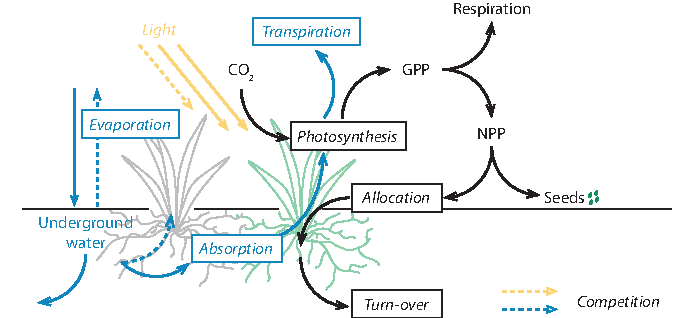
\includegraphics[width = 1\linewidth]{./1_Introduction/graphics/model_cycles.pdf}
\caption{Model overview. \textcolor{myBlue}{Water} and \textbf{carbon} cycles are represented. Processes are represented framed and in \textit{italic} by contrast with pools that are not framed and in regular fontface. Dashed arrows indicate loss of resource (for the \textcolor{myGreen}{focal plant}) due to competition.}\label{fig:overview}
\end{figure}


\subsection{State variables}

\paragraph{Scales}
In mountain grasslands individuals (tillers) generally do not grow big and interact only with close neighbours and form little patches. And thus it is possible to represent a rich community at a fairly small scale ($\approx$ dm or m), but the spatial resolution should be relatively fine ($\approx$ cm) to capture inter-individual interactions. Because the model is intended to explore climate change impact on mountain grasslands, it can run on multiple growth seasons separated by snow-covered periods, but must also integrate the intra-seasonal variations at daily scale. Mountain weather (mostly temperature) is known for its large hourly variations, it would, however, require too much computational power to consider such variations. In addition to this argument, we believe that even though they imply physiological flexibility and specific strategies for plants experiencing these conditions, they will not have a huge impact on overall community dynamics changes caused by the climate change. That why hourly variations will not be considered and physiological processes are estimated at the daily timescale.

\paragraph{Plants} The plants are described in the model by state variables described in table \ref{table:state_var_plant}. The best way to understand how plant are represented is to imagine two homogeneous cylinders on top of each other, the shoot cylinder varying in radius and height representing the light acquisition (and shading) zone, and the root cylinder varying only in diameter (because of shallow soil in mountain ecosystems) representing the water acquisition zone. These cylinders are centred on cells of the torus simulation plan.\\
\begin{marginfigure}
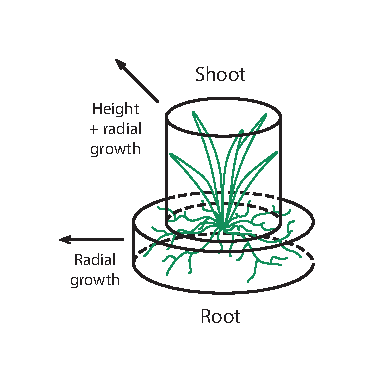
\includegraphics{./Figures/plant_geometry_m.pdf}
\caption{Plant geometry and growth axis.}
\end{marginfigure}
\indent In addition to classic variables (age, position, height, diameter, shoot and root biomasses) the plants are described by traits, that can be species-specific or non-specific, others are variable (SLA, SRL) and depend on particular traits that are unique to this model: the \textbf{ratio between active tissue and structural tissue} (in shoot and root) (variables $\frac{act}{str}_{ag}$ and $\frac{act}{str}_{bg}$ in table \ref{table:state_var_plant}). This couple of traits come from the evidence that numerous trade-off observed in leaves can be explained (at least partially) by this allocation trade-off between active tissue producing organic matter, but increasing respiration, and structural tissue that increase tissue lifespan.

%TAble of plant state variables
\begin{table2*}
\caption{State variables of individual plants} 
\label{table:state_var_plant}
%\begin{center}%
\begin{tabular}{l|l|c}
Variable & Description & Unit \\ 
\hline 
x & x position on the grid & cells \\
y & y position on the grid & cells \\
age & age & days \\
sp & species & - \\
$BM_{ag}$ & above-ground biomass & g \\
$BM_{ag_sen}$ & senescent above-ground biomass & g \\
$SLA_{sen}$ & senescent above-ground biomass & $cm^{2}.g^{-1}$ \\
$BM_{bg}$ & below-ground biomass & g \\
stem & stem biomass & g \\
$\frac{act}{str}_{ag}$ & above-ground active on structural biomass ratio & g/g \\
$\frac{act}{str}_{bg}$ & below-ground active on structural biomass ratio & g/g \\
h & height & cm \\
r & shoot radius & cm \\
r\_r & root radius & cm \\ 
$light_{exp}$ & above-ground potential resource availability & gH2O.leaf area\\
$water_{exp}$ & below-ground potential resource availability & gH2O.root area\\
\end{tabular} 
%\end{center}
\vspace*{0.5cm}
\end{table2*}

%little scheme to show what it looks like

\paragraph{Species} Plants are characterised by state variables that describe them individually, but they also share common characteristics with individuals of the same group, (we will refer as \textit{species} to talk about this group in the rest of the document even though it could be a group at another scale (i.e. population, clones). These species are the groups present in the meta-population and that can invade the simulated ecosystem. There are described by multiple traits characterising the strategy of the species (table \ref{table:state_var_species}).


%TAble of plant state variables
\begin{table2*}
\caption{Species traits}
\label{table:state_var_species}
\begin{center}
\begin{tabular}{l|c|c|l}
Trait & Range (close range) & unit & trade-off or strategy\\
\hline 
seed mass & (0.00001 - 0.001) & g & seed ouput vs seedling productivity\\
maturity & - & green biomass & flowering time vs reproduction potential\\
fract\_dev & 0-1 (0.05-0.6) & - & blooming vs persistence\\
fract\_rep & 0-1 (0-1) & - & reproduction vs persistence\\
geometric constant ($k_{g}$) & (0.1 - 20) & - & competition sensitivity vs self-shading\\
plasticity stability & 0-1  (0.8-1) & - & genetic information vs experience\\
initial water resource & (0.001 - 0.05) & $gH_{2}O.cm^{-2}$ & water resource niche\\
initial light resource & (0.001 - 0.05) & $gH_{2}O.cm^{-2}$ & light (in $H_{2}$ equivalent) resource niche\\
$\frac{act}{str}_{ag,d}$ & (0.03 - 0.3) & $g.g^{-1}$ & active vs structural tissue\\
$\frac{act}{str}_{gg,d}$ & (0.03 - 0.3) & $g.g^{-1}$ & active vs structural tissue\\
mean temp. & (0 - 5) & \celsius & early vs late germination\\
germination rate & 0-1 (0.5 - 1) & - & good season bet-hedging\\
thickness & 	(0.012 - 0.05) & cm & WUE vs light efficiency (not in this version)\\
\end{tabular} 
\end{center}
%\vspace*{0.5cm}
\end{table2*}
%table of species traits. trait, range, distribution, trade-off or strategy associated.

\paragraph{Seed-bank} The seed-bank is the transition state between the different seasons. Individuals may persist thanks to stored resources, but they can also reproduce by the production of new individuals. A lot of grasses use clonal reproduction, in addition, or replacement of sexual reproduction. This type of reproduction is characterised by a persistent link between the newly produced individuals and the parent one that allows the two to communicate and exchange resources. Such dynamics are complex and costly to represent as the link between ramets must be stored and strategies defined for the resource distribution (see Oborny 2012) for more details on clonal growth modelling). To avoid too much complexity, it is possible to approximate the representation of clones to big seeds with little dispersion around the parent plant\footnote{This would take advantage of dispersion kernels. Not implemented in the current version. Dispersion is uniformly random within the simulation plan}. For this reason, reproduction mechanism is reduced to sexual reproduction mechanism with the production of "seeds". Seeds are stored in the seed-bank and only defined by their species and positions. 

\paragraph{Soil}
\begin{marginfigure}
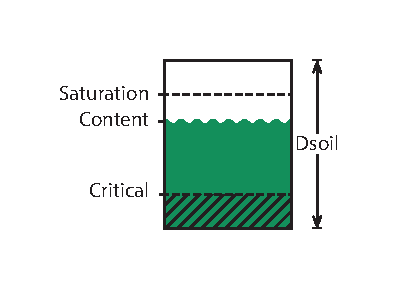
\includegraphics{./Figures/soil_section_m.pdf}
\caption{Soil section.}
\end{marginfigure}
The soil is an important aspect of the model as it drives (with the precipitations) the water competition between individuals. It is however limited, as in numerous vegetation models, to a grid characterised by its capacity to retain water, and its depth. Only the first component (water retention capacity) is spatially variable and is described by the critical water content (minimum soil water content), the saturation water content (maximum water content, the water non absorbed leaves the system we assume the same root depth for all species), and the current water content (temporally variable, depending on competition, precipitation and evaporation, between the critical and the saturation water content) only dynamic variable among the three.

%table of soil state variables

\subsection{Process overview and scheduling}

As mentioned the model runs at a daily step to capture individual responses to conditions and over multiple seasons to capture long temporal dynamics. Some processes occur (or are evaluated) at the daily time-step, some at the season time-step. The following ordered list presents the different processes and the scheduling over days and season of one simulation.\\
\indent One season can be divided into the following parts:
\begin{marginfigure}
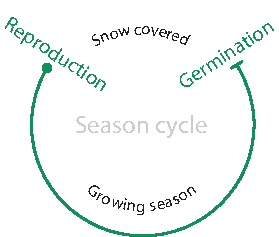
\includegraphics{./Figures/season_cycle_m.pdf}
\caption{Seasons cycle in \model.}
\end{marginfigure}
\begin{itemize}
\setlength\itemsep{0em}
\item \textit{germination}: marks the beginning of the season when the ground is no more snow-covered;
\item \textit{growing season}: consists in daily processes like competition, production of organic matter (OM), allocation, and death lottery;
\item \textit{reproduction-invasion-persistence}: marks the end of the season when the first persistent snow-fall occurs. OM invested in reproductive tissues turns into seeds that are sampled to create the seed-bank. Seeds from the meta-population may integrate the seed-bank. Persistent perennial loose most of their biomass but storage (and eventually stem) and regrow from stored organic mass at the beginning of the following season.
\end{itemize}

The \textit{growing season} part consists in all processes evaluated every day of the growing season. These processes are:
\begin{marginfigure}
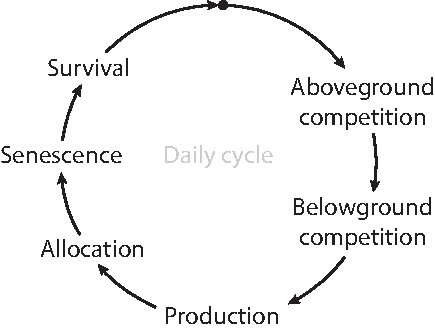
\includegraphics{./Figures/daily_cycle_t.pdf}
\caption{Processes in order during the daily cycle.}
\end{marginfigure}
\begin{itemize}
\setlength\itemsep{0em}
%\item \textit{resistance allocation}: the stored OM (in seeds or in storage tissues) are either invested in resistance molecules or in development;
%\item \textit{freezing}: frost damage on plants;
\item \textit{light competition}: the individual potential photosynthetic activity is computed based on average daily light and shoot properties;
\item \textit{water competition}: evaporation and the individual water update (and potential water uptake) are computed based on potential transpiration, water availability and potential evaporation;
\item \textit{production}: respiration and production are computed to give the net productivity in OM;
\item \textit{senescence}: based on lifespan a part of tissue is no longer active.
\item \textit{death}: death of individuals based on their age and their desiccation stage (number of consecutive days with negative growth).
\item \textit{allocation}: allocation of produced OM to the different carbon pools of the plant.
\textcolor{Gray}{\item \textit{grazing/cutting}: (optional) grazing or cutting of plants to a certain height. The grazing can be selective.}\footnote{remarks in \textcolor{Gray}{grey} are features or components implemented in the model but not used and-or calibrated.}
\end{itemize}


\section{Design concepts}

\subsection{Design concepts}
This part clarifies the rules that drive the dynamics of the model.

\paragraph{Emergence} 
The purpose of the model is to understand the rules that drive the community responses. We tried making the community dynamics emerge from the underlying processes of plant growth, resource use, and reproduction. That means that population dynamics are at least partially emergent from the surviving and reproducing individuals.
\textit{Partially} emergent because it depends on the invasion rules applied to the system. The traits and biomass distribution that describe the community are completely emergent from the individual traits exposed by the individuals and their relative biomass and abundance.
\begin{marginfigure}
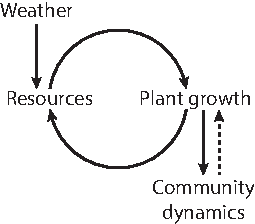
\includegraphics{./Figures/emergence.pdf}
\caption{Population dynamics emerging from plant growth and weather.}
\end{marginfigure}

\paragraph{Adaptation} Plants have in theory many options to adjust their phenotype and increase their fitness in response to changes in environmental conditions (resource availability, temperature, ...). High diversity of mountain grasslands suggests that multiple strategies coexist and that individuals do not change to converge toward a unique strategy. These strategies are set up at the species level by the species-specific traits (see table \ref{table:state_var_species}). Therefore, individuals may only adapt morphological traits but not strategic traits (unless there is an epigenetic mechanism added). These morphological traits are the relative biomass of shoot and root, the relative proportion of active and structural tissues in each leaf, and roots (controlling respectively the SLA and SRL and the overall resource acquisition cost)\footnote{and optionally the proportion of stored OM dedicated to frost resistance and not to growth}. Geometry traits (distribution of leaves and roots within space) are not considered plastic as grasses have far less control over their geometry than forbs or trees. Root distribution plasticity has been shown to greatly improve the individual and community productivity (Gemini article), but to keep the model (and implementation) simple we will ignore root distribution plasticity and foraging strategies to focus on allocation problems instead of spatial distribution questions. Shallow soils and relative small rooting zone are also arguments to ignore spatial distribution plasticity for roots.

\paragraph{Fitness}
\begin{marginfigure}
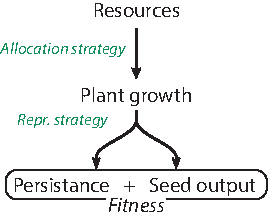
\includegraphics{./Figures/fitness.pdf}
\caption{Fitness emerges from the plant growth and the plant reproductive strategy.}
\begin{footnotesize}
The plant growth is the result of the interaction of the resource levels, the plant strategy, and the competitors.
\end{footnotesize}
\end{marginfigure}
In the model, the realised fitness can be estimated as the capacity of plants to maintain themselves or their descendants through time. It emerges from the productivity, allocation to storage or reproductive carbon pools, and survival. Assessing fitness as the average number of persistent individuals is, however, a bit hazardous in simulations limited in time and to a relatively small spatial scale. Plus, plants cannot easily make a prediction of such variable to adjust their phenotype. They need a proxy function for fitness that integrates measures of external conditions to evaluate the best strategy to develop. As said above, this strategy should be a composite between the species strategy and individual adjustment specific to the individual experience of the environment. Plant fitness is estimated by individual plant thanks to a gain function integrating current phenotype, species strategy, and projection of future conditions. This gain function can take multiple forms and be more or less constraint. In the context of the model, the function should include a measure of productivity that relies on the principle of functional equilibrium - that is the allocation of organic matter to maintain the balance between the shoot activity (transpiration) and root activity (water uptake). This equilibrium can be achieved by changes in shoot:root ratio only, or also changes in active over structural tissues ratio. Further details about the gain function are discussed in the dedicated paragraphs (\ref{par:allocation}). A more complex form of functional equilibrium incorporating nutrients (like nitrogen) could be added to the framework of this model.

\paragraph{Prediction} Adaptation or plasticity mechanisms imply that agents have an insight of what will be the future. In \model we consider that plants have two main sources of information. The first source of information is the genetic information. Indeed, the evolutionary process of genotype selection has led to the selection of genotypes adapted to the local conditions. This selection relationship can be seen as a link between environmental conditions and genetic information. Because plants cannot fully predict future environmental conditions, they grow following (at least partially) the plan contained in genetic information that match conditions where previous generations grew in.  This is an internal \textit{a priori} information about the external conditions. If the conditions where the seed grows change from the conditions its genotype has been selected for, the genetic information does not fit the environmental conditions is not sufficient enough to build a working phenotype. In this case, if the plant has a plasticity capacity, it can integrate the second source of information, in the form of the experienced conditions, to its "a priori" and forge a new estimation of what conditions will be. One question emerges to this idea is: how to create an image of future conditions and how to balance the genetic \textit{a priori} information with the experienced information? This balance can be described by a term of "reactivity" that describes the relative weight of genetic and experienced information. A reactive species will give a higher weight to experienced condition information, whereas a stable species will give a higher weight to genetic information.\\
\indent The way the two source of information are brought together and used to define the plant phenotype is at the core of plant strategy and is the main feature of the model \model.
\begin{figure}
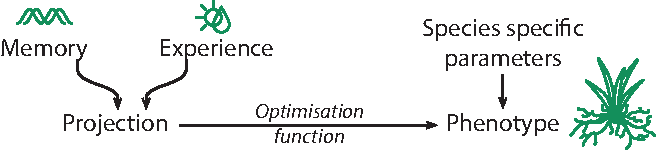
\includegraphics{./Figures/memory2phenotype_t.pdf}
\caption{Genetic and perceived information are both considered to determine the phenotype.}
\end{figure}
%\indent From that mechanism we can define two terms: the \textbf{climatic niche center} of a species is the \textit{a priori} information on climatic conditions, and the \textbf{plastic capacity} of a species is both its reactivity and its capacity to overcome the plasticity cost and invest in required tissues.
%Individuals do not estimate directly their fitness. They have however a way of estimating how well they perform depending on the level of resources they estimate. This measure is essential in plasticity mechanism as it drives plasticity. This measure is dependent on the plasticity mechanism chosen. Indeed plasticity can be approached in different ways that are discussed later, one mechanism consists in maintaining the \textit{functional equilibrium}, in this case, the fitness information is approached by the relative balance between above-and below-ground activities. The other mechanism is the \textit{optimisation}, that implies a more complex estimation of productivity, respiration, tissue turn-over and death changes and gives a more detailed approximation of individual fitness.
%\paragraph{Prediction and adaptation} As explained above, the "incomplete fitness proxies" used in the plasticity mechanisms require estimation of above- and below-ground activities, based on their trait values (SLA and SRL) and on an estimation of future external conditions (temperature, water availability and light availability). The originality of our approach is to make this estimation depending on both species-specific parameters and individual experience. The conditions are estimated as the weighted mean between the species-specific genetic \textit{a priori} on resource availability and the potential resource availability normalized over exchange area. This makes the estimation by one individual depending both on the species-specific "environmental niche" and the competition effects on resources. Moreover, this mechanism, because it includes relative weight to the two sources of information, allow multiple strategies for the estimation of external conditions and so on how to cope with resource levels variation.
%
%\paragraph{Adaptation} Adaptation is central in the model as we believe it explains a lot of intra-specific variability in mountain grassland ecosystems (cite Albert and others)
\section{Details}

Further details on daily mechanisms are described in the following paragraphs.


\begin{marginfigure}
%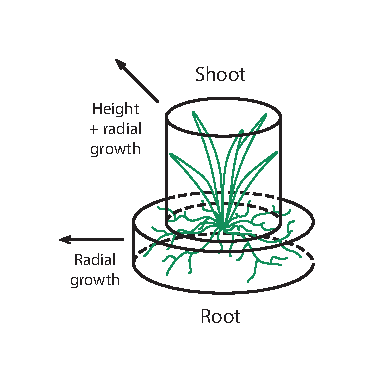
\includegraphics{./Figures/plant_geometry_m.pdf}
\caption{Overview of the model inputs and outputs.}
\end{marginfigure}

\subsection{Initialisation}
The model doesn't need particular initialisation if the state of the community species pool, the seedbank, and the soil are given as inputs. Otherwise, a set of \textit{E(n/s)} individuals are created from a set of \textit{s} species (randomly generated if not given) and randomly positioned on the soil grid, where \textit{s} and \textit{n} are respectively the number of species and the approximate number of individuals within the grid. Soil grid is also randomly generated within default ranges for critical and saturation water contents then slightly smooth, and homogeneously filled ($filling = \frac{w_{cont} - w_{crit}}{w_{sat} - w_{crit}}$).
 
\subsection{Inputs}
\model needs system state information (individuals, species, seed-bank and soil) and climate data. If the state of the system is not completely given, then the complete state is generated in the initialisation. The daily climate data at must contain the following fields:
\begin{itemize}
\setlength\itemsep{0em}
\item \textit{date};
\item \textit{radiance}, in $Watt.m^{2}$;
\item \textit{precipitation}, in mm;
\item \textit{mean temperature}, in K;
\item \textit{mean day temperature}, in K;
\item \textit{min temperature}, in K;
\item \textit{max temperature}, in K;
\item \textit{relative humidity} in \%;
\end{itemize}
Vapour pressure deficit is then computed from temperature and relative humidity.\\
\indent The climate data must explicitly differentiate the seasons (delimited by the first day of the year without snow and by the first day of the second semester with snow).

\subsection{Submodels}\label{subsection:submodels}

\paragraph{Germination} Individuals from the seed-bank randomly germinate according to their species-specific germination rate. Germination consist of investing a percentage ($mob$ parameter) of the seed mass into shoot and root biomass according to default traits. This is coupled with a round of random seed death following uniform law of parameter $seed_{surv}$. Living non germinating seeds stay in the seed-bank until the next season.\\
%
%\vspace{0.5em}
%\paragraph{Freezing resistance allocation} Resistance mechanisms are important for plants to invade harsh environments with perturbations such as grazing of frost events. Investment in free organic compounds is shown to provide resistance to frost. The concentration of such compounds is time variable and closely related to temperature. Other mechanisms morphological, structural, physiological can also play a role in frost resistance. For the sake of simplicity we will limit this aspect to the investment in circulating agents. Moreover, this aspect is crucial, indeed  because the frost risk is high at the beginning of the season, the choice of investing in resistance molecules instead of growing tissues is a strategy choice. Species can then be differentiated on a earlier growing/high frost risk - late growing/low frost risk axis, depending on their estimation of minimal temperature. Minimal temperature is estimated the same way other resources levels. Available stored biomass is invested in frost resistance is the estimated mean temperature is below 3\celsius .\\
%
% 
%\paragraph{Freezing} The freezing damages are calculated based on the concentration of organic matter dedicated to frost resistance is the plant. The LT50 (temperature at which 50\% of biomass is lost) is proportional to the concentration of resistance molecules compare to overall biomass. Daily leaf biomass lost due to frost is computed as follow:
%
%
%\begin{align}
%k_{frost} &= log(1/dam_{-1} - 1)/(-1 - LT_{50})\\
%dam &= \frac{1}{1 + e^{k_{frost}(T_{min} - LT_{50})}}
%\end{align}

\textbf{Daily processes}

\paragraph{Light competition}Light competition is central to all vegetation model as it constrains the photosynthetic activity and so plant growth. To avoid costly calculation of ray propagation we assume vertical homogeneous top radiation. Relief and orientation effects are taken into account in the computation of irradiance data.\\
Light competition sub-model allows calculation of individual potential photosynthesis activity and light at soil surface for evaporation calculation.\\
Competition for light is calculated independently for each pixel, potential photosynthetic activity is then aggregated at the individual level. Each pixel can be seen as a column of homogeneous layers containing at least one individual (top layer). For each layer, the light transmission is computed based on leaf density.


\begin{marginfigure}
\begin{tikzpicture}
\begin{axis}[marginplot,
legend style
={at={(1, 1.1)},
anchor=south east,
draw = none},
samples = 40,
%restrict y to domain=-300:700,
ylabel = $I_{h}$,
xlabel = $h$
%extra x ticks={0.618},
%extra x tick style={grid=major}
]

\addplot[black][domain = 0:10 ] {120 * exp(-1*x)};
%\addplot[gray][domain = 0:1 ] {(1/(0.022 * 1)) * ((1/0.05 - 1)*x) - %(7*exp(7*x) + 0.03)};
%\legend{$I_{h}$}
\end{axis}
\end{tikzpicture}
\label{fig:derivaives}
\caption{Net gain function and its first derivative.} Looks like there is some kind of mismatch here.
\end{marginfigure}

\begin{equation}\label{eq:Ih}
I(h) =  I_{0} e^{-LAI(h)}
\end{equation}

where $LAI(h)$ is the cumulative LAI at the bottom of layer \textit{l} (between $h$ and $h+\Delta_{h}$) defined as the homogeneous layer delimited by the top of consecutive individuals in the same pixel. The LAI is calculated like this:
\begin{equation}\label{eq:LAI}
LAI(h) = LAI(h+\Delta_{h}) +   \Delta_{h} . pix\_width^{2} \sum_{i\ in\ l}d_{i}.coverage_{i, p}
\end{equation}
where $d_{i}$ is the individual leaf area density corrected by the coverage ($0< coverage =< 1$) of the pixel $p$ by the plant $i$, $\Delta_{h} = (h_{l} - h_{l-1})$ is the height of the layer $l$.\\
Following Thornley and Johnson, the potential photosynthetic leaf activity is calculated as:


\begin{marginfigure}
\begin{tikzpicture}
\begin{axis}[marginplot,
legend style
={at={(1, 1.1)},
anchor=south east,
draw = none},
samples = 1000,
%restrict y to domain=-300:700,
xlabel = $I (W.cm^{2})$,
ylabel = $P_{leaf} (gCO_{2}.cm^{-2}s^{-1}) check that$
%extra x ticks={0.618},
%extra x tick style={grid=major}
]

\addplot[black][domain = 0:0.04 ] {(\paralpha * x * \parPmax ) /(\paralpha * x + \parPmax ) };
\legend{}
\end{axis}
\end{tikzpicture}
\label{fig:derivaives}
\caption{Photosynthetic saturation function}
\end{marginfigure}

\begin{equation}\label{eq:Pleaf}
P_{leaf}(h) = \frac{\alpha. I_{leaf}(h).P_{max}}{\alpha I_{leaf}(h)+P_{max}}
\end{equation}
where $I_{leaf}(h)$ is the light absorbed by the leaf at height $h$, $\alpha$ the initial slope of the light response curve and $Pm_{i}$ the maximum photosynthetic rate per unit of area and unit of time.
% where $I_{leaf}$ is the light absorbed by the leaf and the photosynthetic potential rate $Pm_{i}$ is linearly related to active biomass per leaf area as follow:
%\begin{equation}
%Pm_{i} = min(P_{slope} \frac{Leaf_{Act_{i}}}{Area_{i}}, P_{max})
%\end{equation}
$I_{leaf}$ is the radiance at the leaf surface, derived by correcting the radiance at the top of the layer following the equation used in Taubert with the extinction and transmission coefficients $k$ and $m$:

\begin{equation}
I{leaf}(h) = \frac{k}{1-m}I(h)
\end{equation}

The equation \eqref{eq:Pleaf} can be integrated over the leaf surface by mixing it with equations \eqref{eq:Ih} and \eqref{eq:LAI} to give the total potential photosynthesis for layer $l$ in pixel $p$:
\begin{equation}\label{Ppixlay}
P_{leaf}(p,l) = d_{i}.coverage_{i, p}.\Delta_{h}(l)\int_{h_{bottom}}^{h_{top}}P_{leaf}(h)
\end{equation}
%
%\begin{equation}
%P_{leaf}(l) = \int_{h_{l-1}}^{h_{l}}P_{leaf}.dLeaf = Leaf_{area}\left[- Pm_{leaf}.log(|m.Pm_{leaf} - Pm_{leaf} - \alpha.I_{h(leaf)}|)\right]_{h_{l}}^{h_{l-1}}
%\end{equation}

the total leaf potential photosynthesis is then calculated as follow:
\begin{equation}\label{eq:PS_pot}
PS_{pot} = \sum_{p\ in\ shoot}\sum_{l\ in\ pixel}P_{leaf}(p,l)
\end{equation}
\indent Potential photosynthesis must then be converted to potential transpiration to define the water demand. The conversion from photosynthesis to transpiration is done by dividing the potential photosynthesis by the water use efficiency ($WUE$). The potential activity of leaves are also dependent on the regulation of stomata so the transpiration can be written:
\begin{equation}
transp = \frac{PS_{pot} . g_{red}}{WUE}
\end{equation}

\textcolor{Gray}{\paragraph{Stomatal regulation} Photosynthesis depends on gazes exchanges at the leaf surface. These fluxes result from relative concentration in carbon dioxide and water, and from the stomatal conductance. Stomatal conductance is reduced and limits productivity when vapour pressure deficit is too high \sidenote{$g_{red}$ is set to 1 for current version to avoid potential problems between allocation and regulation}. A linear relationship describe this relationship:
\begin{equation}
g_{red} = 1+ VPD_{g\_red}
\end{equation}}

\paragraph{Evaporation} Potential evaporation is calculated for each pixel depending on the light at soil surface:

\begin{marginfigure}
\begin{tikzpicture}
\begin{axis}[marginplot,
legend style
={at={(1, 1.1)},
anchor=south east,
draw = none},
samples = 500,
%restrict y to domain=-300:700,
ylabel = $\beta$,
xlabel = $\theta$,
extra x ticks={0.8},
extra x tick style={grid=major}
]

\addplot[black][domain = 0:0.8 ] {(1/4) * (1-cos(deg(x/0.8 * pi)))^2};
\addplot[black][domain = 0.8:1 ] {1};
%\legend{$I_{h}$}
\end{axis}
\end{tikzpicture}
\label{fig:derivaives}
\caption{Evaporation  limitation function.}
\end{marginfigure}

\begin{align}
 \beta &= 0.25 * (1 - cos(\frac{\theta}{\theta_{sat}} * \pi))^{2} & if water_{cont} \le water_{sat}\\
 \beta &= 1 & otherwise\\
 PET &= 0.0023. \sqrt{(T_{max} - T_{min})} * (T_{mean} + 17.8)\\
 evap &= PET . \beta . I_{surface} . daylength
\end{align}

\paragraph{Water competition} Water competition is also computed at the pixel level. To determine the water uptake, first the individual water demand is computed as the minimum between the transpiration and the potential water uptake. Transpiration demand per pixel is easily calculated by dividing the total potential transpiration by the volume in the pixel $V_{i,p}$ over the overall root volume $V_{i}$. Water potential uptake is the product of root area in the pixel and root water uptake rate reduced by the water availability reduction factor $U_{lim}$, leading to the water demand for individual $i$ in pixel $p$:
\begin{align}
transp_{i}(p) &= transp . \frac{V_{i,p}}{V_{i}}\\
Wpot_{i}(p) &= Root_{area}(p).U_{max}.U_{lim}\\
Wdem_{i}(p) &= min(transp_{i}(p), Wpot_{i}(p))\\
\end{align}
where, the limitation function $U_{lim}$ is defined as in \parencite{reineking_environmental_2006}:

\begin{marginfigure}[-40pt]
\begin{tikzpicture}
\begin{axis}[marginplot,
legend style
={at={(1, 1.1)},
anchor=south east,
draw = none},
samples = 100,
%restrict y to domain=-300:700,
xlabel = $\theta$,
ylabel = $U_{lim}$
%extra x ticks={0.618},
%extra x tick style={grid=major}
]

\addplot[black][domain = 0.21:0.99 ] {exp(\parbetazero * (1/(1-0.2) - 1/(x-0.2))) };
%\legend{Water limitation}
\end{axis}
\end{tikzpicture}
\label{fig:derivaives}
\caption{Water uptake limitation response function to soil saturation}
\end{marginfigure}

\begin{align}
U_{lim} &= exp\left(\beta_{\theta} \left( \frac{1}{\theta_{s} - \theta_{crit}} - \frac{1}{\theta - \theta_{crit}}\right)\right) & if \theta < \theta_{crit}\\
 &= 0 & otherwise
\end{align}

%Where $U_{i}$ is related to the maximum water uptake $U_{max}$ and to the the $\frac{Root_{Act_{i}}}{Area_{i}}$ as in equation \eqref{eq:Pleaf}.\\
The total water demand per pixel is then the sum of all individual water demand of the pixel and potential evaporation. If the total water demand exceeds the total water availability ($W_{av}$ product of water content and soil volume in the pixel) then the available water is distributed proportionally to the individual demand.\\
\begin{equation}\label{eq:water_uptake}
Wup_{i} = Wdem_{i} . \frac{Wdem_{total}}{min(Wdem_{total}, W_{av})}
\end{equation}


\indent The potential water uptake ($Wpup$), non limited by the transpiration is calculated the same way but considering $Wdem_{i} = Wpot_{i}$ in equation (\ref{eq:water_uptake}).\\
\indent Because the water competition is computed at the pixel level, there is no compensation between two pixels containing respectively not enough and too much water.\\
\indent No radial flow of water between pixel is implemented in the model. This simplification leads inevitably to edge effects, but allows simpler implementation and is partially covered by the effect of the pixel size. Indeed, increasing pixel size would have similar effect in the pixels at the border of the rooting zone than radial flow because it would increase the potential water pool plant has access to.\\

\indent Once potential and realised transpiration and water uptake are computed, 
plant productivity can be calculated.


\paragraph{Production, and respiration} Following previous vegetation models, the respiration is decomposed in growth respiration and maintenance respiration. The first is function of trait values, biomass and temperature:
\begin{equation}
R_{m} = \left(R_{act}.\left(Act_{ag} + Act_{bg}\right)\right) . daylength . T_{effect}
\end{equation}
where $R_{act}$ is the respiration rate of active tissues, and $Act_{ag}$ and $Act_{bg}$ are the active biomass pools in shoot and root.\\
\indent Net Primary production (in $CO_{2}$ equivalent) can then be calculated the difference of GPP and respiration, then converted in OM production thanks to tissue carbon content (under the assumption of fixed carbon content for leaf and roots between species):
 \begin{align}
 NPP_{carbon} &= (1- R_{g}) . (WUE . min(w_up, trans_p) - R_{m}) - BM_{total} * Pl_cost\\
 NPP_{OM} &= NPP_{carbon} . (12/44) / TCC
\end{align} 
Here $R_{g}$ is a fixed parameter but is set to $0$ if the difference between gross productivity ($GPP = WUE . min(w_up, trans_p) - R_{m}$) and maintenance respiration is negative. $Pl_{cost}$ is the plasticity cost as calculated in the dedicated paragraph below.

\paragraph{Temperature effect} Temperature has a effect of plant activity, this effect can be modelled by a bell shape function around an optimum value of 20 \celsius . See Lohier for details.


\paragraph{Condition estimation} The projection of environmental conditions is central in any implementaion of phenotype plasticity. Differences between the current perception of environment and the projections lead to adjustment of phenotype to increase fitness. In the model \model this projection results from hte averaging of two key concept: memory and perception. The latter is relatively simple to understand and corresponds to the perceived resource availability computed as the mean potential exchange rate per unit of area (total leaf or root area) and per hour(the hourly measure is used instead of daily measure to simulate the ability of plant to perceive the photoperiod. This is an easy way of taking into account one aspect of seasonality without complicating the model. However, it also reduce the range of memory and its impact to determine the phenotype, as an additional information would be needed to define the optimum phenotype: the day length).:
\begin{align}
light_{exp} &= \frac{transp}{exhange area_{ag}}\\
water_{exp} &= \frac{Wpup}{exchange area_{bg}}\\
\end{align}
The former is related to the species (or group) history and result from processes of selection and acclimation. It is the default projection of resource availability when the plant is not plastic. 
\begin{align}
light_{est}(t+1) &= (1 - \tau).light_{exp}(t) + \tau . light_{memory} . daylenght(t+1)\\
water_{est}(t+1) &= (1 - \tau).water_{exp}(t) + \tau . water_{memory} . daylenght(t+1)
\end{align}
\indent Because these are supposed to be expected conditions for the future, other formulation can be used instead of an average that is likely to introduce a lag in estimations. For example the following equation allow for a more stable projection that better fits the slower process of plant physiology adjustments:
\begin{align}\label{eq:projection_alt}
light_{est}(t+1) &= ((1 - \tau_{react}).light_{exp}(t) + \tau_{react} . light_{est}(t))((1 - \tau_{amp}) + \tau_{amp} . light_{memory}) . daylenght(t+1)
\end{align}
with $\tau_{amp}$ and $\tau_{react}$ being respectively amplitude and reactivity where only $\tau_{amp}$ is used in the first equation. Such solution could limit sensitivity and phenotypic instability. IN addition, such formulation would also better capture the accumulation of stress signals and would lead to a softer and more stable phenotypic shift.\\
\indent The estimation of external conditions as expressed here is then used to select the best allocation scheme during the allocation process. Limited here to levels of two resources (light and water), this estimation equation could be extended to other mechanisms such as herbivory risk, frost risk, humidity impact on water pressure deficit.\\

\paragraph{Allocation} \label{par:allocation}
Allocation is primordial in plant development and ontogeny. The following paragraph detail the implementation of the plastic allocation in \model.\\

\textbf{Maturity:} For most of plants the development cycle is divided in two phases of different durations: the vegetative phase when plant growths organs to gather resources and product OM, and the reproductive phase when plant take advantage of these organs to accumulate carbon and invest them in reproduction mechanisms. Plants are considered mature (they switch from vegetative to reproductive phase) in \model when the phenologic variable has reach a species specific threshold. The phenologic variable can be either the age, the height, the biomass, degree.days, in the current version total living biomass is used as trigger for reproductive phase.\\

\textbf{Allocation to supporting tissues:} Even-though grasses do not grow tall vegetative parts like trees, some grow vertically and they are exposed to stronger winds than most of forest. Therefore they need structural supports\sidenote{This supporting tissue mechanic is also needed to avoid exponential growth rate.}. Not all grasses grow stem, but they'll have stronger central vein in their leaves to structurally support the weight of leaves. In addition shoots and roots also need supporting tissues for water transport, for this reason the minimal mechanical support needed is calculated as a function of total living biomass:
\begin{equation}
support = \alpha . (BM_{ag} + BM_{bg})^\gamma
\end{equation}
where $\alpha$ and $\gamma$ are allometry coefficients.\\

\indent At each time step we must determine what fraction of new OM will be allocated to tissues growth while the remaining will support these need tissues. This leads to an optimisation problem numerically solved by the function \texttt{uniroot}.\\
%Despite the ambiguity in the name, there is a fundamental difference between structural tissues and supporting tissues: the former is part the individual organs and  
%\indent To avoid complex allocation optimisation problem, the allocation of supporting tissue is done before any other allocation. Is the support is not sufficient, no organic matter can be invested in vegetative development. The biomass the plant needs to invest in the stem is defined as:
%\begin{equation}
%\Delta_{stem} = max(support - (stem + Str_{ag}), 0)
%\end{equation}
%where $Str_{ag}$ is the structural biomass in shoot.\\
\begin{figure}
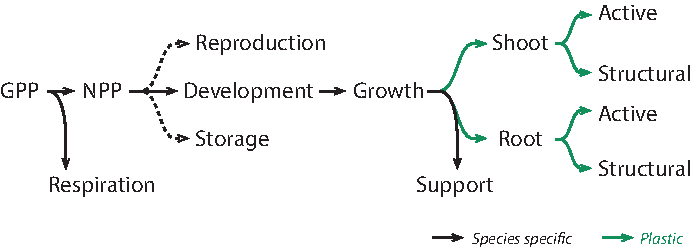
\includegraphics{./Figures/allocation_path_t.pdf}
\caption{Allocation of produced organic matter to different processes and pools.}
\end{figure}

\textbf{Allocation to organs:} Allocation of produced organic matter is central in vegetation as it shapes the plant and define the strength of the different organs. There are multiple ways to model the distribution of produced organic matter between the plant organs. We believe that such mechanism has great impact on individual development and response to external conditions, and so on community dynamics. To explore the role of this mechanism, multiple options are implemented. The different allocation algorithms are summarised in table \ref{table:alloc_algo}.\\
\indent There are two major components in the allocation algorithm:
\begin{itemize}
\item the objective function;
\item the plastic dimensions.
\end{itemize}
The \textit{objective function}: it is the function that give an fitness estimation or gain metrics for any given phenotype. This function is used to compute the optimum phenotype (phenotype at which the function is evaluated at the maximum value), or rank alternative phenotypes\sidenote{in this case, if not all possible phenotypes are tested, the solution might be only a local optimum. This is the case in \model.}. \\
The \textit{plastic dimensions}: they are the dimensions along which the individual can move. The space defined by these dimensions is the phenotypic space within which each individual plant can look for an alternative phenotype. They do not necessarily fully define a phenotype since some dimensions of the individual's phenotype can be fixed \sidenote{either by shared parameters of species specific ones.}. \\
\begin{figure}
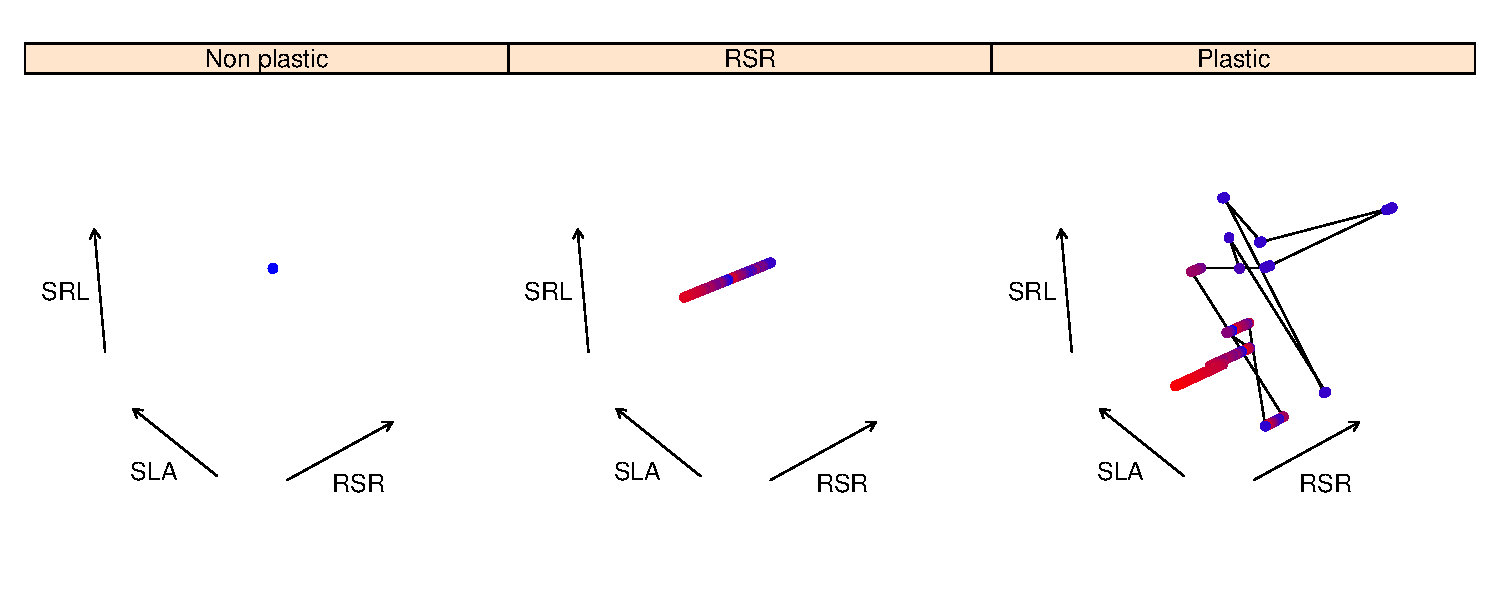
\includegraphics{./Figures/strategy_space_algo.pdf}
\caption{Trajectories of a plant in the trait space depending on the plastic dimensions explored.}
\end{figure}
\indent The objective of this step of the model is to solve the objective function with the unknown variables being the plastic dimensions (RSR, SLA and SRL). In case of simple equations an analytical solution could be used to find an optimum \sidenote{under the condition that such optimum exists. The design of the model should ensure that.}. However, because the analytical solutions are already non trivial and the model is likely to evolve, a numeric solving method is adopted. \textbf{Need to detail the random algorithm.}\\
Also make a note on multiple optimum and the choice for a 'gradient descent" type of algorithm. Also sensitivity at eraly stages 

%TAble of plasticity mech
\begin{table*}
\caption{Allocation algorithms implemented in \model} 
\label{table:alloc_algo}
%\begin{center}%
\begin{tabular}{l|c|c c c}
Algorithm & Objective & variable RSR & variable SLA-SRL & stochastic \\ 
\hline 
No plasticty & $-$ & $\circ$ & $\circ$ & $\circ$ \\
Equilibrium & functional eq. & $\bullet$ & $\bullet$ & $\bullet$ \\
Eq-Fixed & functional eq. & $\bullet$ & $\circ$ & $\bullet$ \\
Optimisation & instantaneous gain & $\bullet$ & $\bullet$ & $\bullet$ \\
Optim-Fixed & instantaneous gain & $\bullet$ & $\circ$ & $\bullet$ \\
\end{tabular} 
%\end{center}
\vspace*{0.5cm}
\end{table*}

\textbf{No plasticity allocation:} this allocation is very similar to classic vegetation model where the biomass is allocated to the different carbon pools according to species specific parameters. But \model differs from other models by the order of the different steps of growth. In this model, the senescence comes between the allocation step and the resource competition-production steps \sidenote{see plastic allocation algorithm for explanation}. The partitioning coefficient are directly computed from species default trait to maintain the phenotype after senescence.

\textbf{Fixed trait allocation:} The fixed allocation supposes the allocation on OM to maintain trait values to fixed species specific values. The shoot:root ratio may however change to maintain functional equilibrium. The shoot root ratio is derived from the following equation of the functional equilibrium:
\begin{align}\label{eq:equilibrium}
SLA . BM_{ag} . light_{est} &= SRL . BM_{bg} . water_{est}\\
\frac{BM_{ab}}{BM_{bg}} &= \frac{SRL}{SLA} . \frac{water_{est}}{light_{est}}
\end{align}
where $light_{est}$ and $water_{est}$ are the estimated resource availabilities.
%
%\subparagraph{Plastic functional equilibrium} This allocation mechanism is also based on the functional equilibrium, however it incorporate changes in traits, that means that the proportion between active and structural tissues in an organ can change. This idea is supported by tha fact that plants change both their shoot:root and their trait values when conditions change. From a perspective with only one allocation dimension (shoot or root in "fixed trait allocation") with three dimensions (shoot or root, active or structural in shoot and in root tissues), the number of constraints must increase to find a unique solution. The functional equilibrium only is not sufficient to define the allocation scheme as multiple solutions satisfy this constraint. The solution is to chose among all possible allocation schemes the closest to the current allocation, the shortest path to functional equilibrium. This is done by minimising the 
% doesn't work for now

\textbf{Plastic trait allocation:} Another approach to allocation is to try to optimize phenotype based on a fitness proxy. This proxy can  be the sum of NPP, tissue turn-over loss and plasticity cost. But in a complex model like \model, plant performance is function of multiple aspects:\
\begin{itemize}
\item individual organ efficiency;
\item relative mass of each organ;
\item balance between organ water exchange activities.
\end{itemize}
And this could be extended to herbivory or frost risks. To take into account all these components, and take advantage of having all processes already made explicit by the implementation in the model, the daily processes of senescence and production are recalculated according to the \textbf{estimation of conditions} and the plant phenotype. This function is used to rank different alternative phenotypes (algorithm detailed below).

\textbf{Plastic trait equilibrium:} An alternative approach can be easily derived from the previous one and extend the principle of the first: the functional equilibrium with plastic traits. This approach consists in using the same algorithm as before but rank phenotypes with a function negatively correlated to the difference between estimated shoot and root activity. Such mechanism would nonetheless require the algorithm to look for close solutions within the allocation space to avoid convergence or drift from species strategy. Having non zero cost of plasticity in this approach should limit the drifting of the plant phenotype.

\textbf{Fixed trait optimisation:} This algorithm takes the idea of the optimisation algorithm but limits the plastic traits to the RSR ratio. If we can expect similar response than the fixed trait equilibrium if we suppose that the equilibrium is the main aspect of plant performance, global efficiency being considered in this case the result may vary.

\paragraph{Plastic algorithm}

Alternative phenotypes are computed from the actual phenotype and random uniform distribution of available organic matter to the main active and structural carbon pools of the plant.\sidenote{talk about the order senescence production, and the way exchange rates are computed.} ... This algorithm has the advantage of being relatively cheap compared to other optimization functions, however, its performances are variables and it is very sensitive to the number of samples used. As a consequence there is a trade-off between model stability and performance as a function of the number of samples (\textit{i.e.} alternative phenotypes) considered.
\begin{figure}
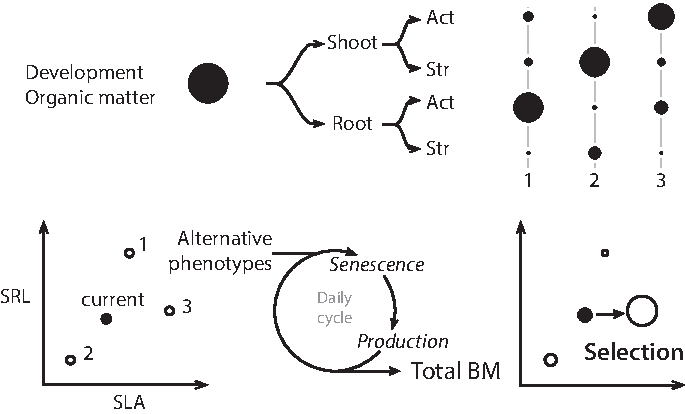
\includegraphics{./Figures/phenotype_ranking_t.pdf}
\caption{Algorithm for the evaluation and selection of randomly generated alternative phenotypes.}
\end{figure}

\paragraph{Plasticity cost}
The limits and costs of plasticity have long been discussed in the related literature. If \model is intended to be used to examine ecological costs and limits, it has to include physiological aspects of plasticity limits. There are two physiological processes involved in the mechanism of altering a phenotype based on changes in external conditions: sensing and signalling. 'Sensing' relates to the capacity of the individual to perceive environmental conditions. This is related to the capacity of the individual to perceive the environment and should, therefore, be considered constant over time. To take into account the cost of precise sensing, the first component of the plasticity cost is proportional to $\tau$.\\
The other component is related to the capacity of the plant to transmit this knowledge of conditions to change the development plan toward a new phenotype. This cost is proportional to the carbon-based distance (calculated as the difference between proportion of active tissues) between the default phenotype and the alternative (during allocation algorithm) or current phenotype.\sidenote{We could imagine cost based not on the default, but the previous phenotype, but it would have lead to large phenotypic shifting and convergence.}\\
Plasticity cost is the sum of both component and is proportional to the total biomass since most of the tissues should have the appropriated cell machinery and are affected b plasticity.
\begin{align}
pc_{maintenance} = (1 - tau) * pc_m \\
pc_{plasticity} = d_{traits} * pc_p
\end{align}
where $d_{traits}$ is the Euclidean distance between default phenotype and the alternative phenotype in the space defined by the proportion of active tissue for shoot and for roots.

\paragraph{Trait update}
Plasticity in trait suggests that trait values are modified in time. Because plants are described by single values (e.g. one SLA value for all leaves), this values must be updated after the plastic allocation. This values could be updated as the average of old tissue value weighted by old biomass and new tissue value weighted by the freshly produced biomass. This, however, would work only if active on structural tissues ratio linearly linked to others traits. This is not the case, it is then simpler to consider that organs have uniform active and structural distribution. This hypothesis suggests that whenever the allocation scheme change, old tissue reallocate their own biomass to follow the new scheme. Nevertheless, to avoid full plasticity allowed by this hypothesis, the changes in trait carbon pool sizes are limited by the produced biomass available for plant development.\\ollowing the following survival probabilities:


\indent From this, supposing homogeneous distribution of active and structural tissues within an organ allows to directly link the size of the carbon pools to average traits by the following relationships:
\begin{marginfigure}
\begin{tikzpicture}
\begin{axis}[marginplot,
legend style
={at={(1, 1.1)},
anchor=south east,
draw = none},
samples = 100,
%restrict y to domain=-300:700,
xlabel = $p_{act_{shoot}}$,
ylabel = $SLA$
%extra x ticks={0.618},
%extra x tick style={grid=major}
]

\addplot[black][domain = 0:1] {1/(\parth *  x * \parrhoas + \parth * (1 -  x) * \parrhoss * \parvts) };
%\legend{Water limitation}
\end{axis}
\end{tikzpicture}
\label{fig:SLA}
\caption{Specific Leaf Area as a function of the proportion in active tissues in shoot}
\end{marginfigure}

%  th_{a} &= \frac{\frac{act}{str}_{s} . th . \rho_{ss}}{\rho_{as} + \frac{act}{str}_{s} . \rho_{ss} }\\
%  s_{a} &= \frac{\frac{act}{str}_{r} . s_{root} . \rho_{sr} }{ \rho_{ar} + \frac{act}{str}_{r} . \rho_{sr}}\\
\begin{align}
  SLA &= \frac{1}{(th .  p_{act_{shoot}} . \rho_{as} + th . (1 -  p_{act_{shoot}}) . \rho_{ss} ) . V_{t}}\\
  SRL &= \frac{1}{(s_{r} .  p_{act_{shoot}} . \rho_{ar} + s_{r}.(1 -  p_{act_{shoot}}) . \rho_{sr}}
\end{align}


\paragraph{Senescence}

Senescence is the process of ageing of tissues. This process usually occurs at the scale of an individual organ (e.g. a leaf), however, \model does not consider organs independently because it would be complex and computationally expensive to follow multiple leaves and roots for all individuals. So the process is considered homogeneous over all tissues. To emulate the senescence process senescence is calculated from the tissues lifespan, giving :

\begin{marginfigure}
\begin{tikzpicture}
\begin{axis}[marginplot,
legend style
={at={(1, 1.1)},
anchor=south east,
draw = none},
samples = 500,
%restrict y to domain=0:1,
xlabel = $P_{act}$,
ylabel = $Lifespan (days)$
%extra x ticks={0.618},
%extra x tick style={grid=major}
]

\addplot[myGreen][domain = 0:0.99 ] {(\parlsszero * (1- x^\parlssone) ) };
\addplot[black][domain = 0:0.99 ] {(\parlsrzero * (1- x^\parlsrone) ) };
\legend{Aboveground, Belowground}
\end{axis}
\end{tikzpicture}
\label{fig:lifespan}
\caption{Lifespan of organs as a function of proportion of active tissues.}
\end{marginfigure}

\begin{align}
sen_{leaf} &= \frac{1}{LLS}\\
sen_{root} &= \frac{1}{RLS}
\end{align}

Because \model does not contain any mechanism preventing plant from growing only  active tissues\sidenote[][5pt]{it was intended to make the WUE negatively correlated to the amount of structural tissue per area.}, it is necessary for this cost function to make this strategy unreliable. The is then expressed as follow:

\begin{align}
LLS &= LSs_{s0} * (1- p_{act_{shoot}}^{LSs_{1}}) \\
RLS &= LSr_{s0} * (1- p_{act_{root}}^{LSr_{1}})
\end{align}


where $LLS$ and $RLS$ are respectively the leaf and the root lifespans calculated as negative log-linear relationships with the proportion of active tissue.\\
\indent Root senescent tissues disappear from the system. Information about senescent aboveground biomass is stored, but senescent biomass effect of light competition is ignored in this version because as it is implemented senescent tissues appear early in plant development and have large negative effect on light absorption.\\
\indent To the natural senescence and artificial cost of having only active tissue, an additional component can be added to the turn-over rate: the negative NPP. In case of negative NPP, the biomass will be taken from the already allocated following the shoot:root ratio. This can lead to a lower overall productivity (negative growth during unproductive periods) but also changes in the equilibrium if tissue have different efficiencies.\\

\paragraph{Death} Death is modelled as in Reineking \parencite{reineking_environmental_2006}. Age and desiccation (negative NPP) are the two reasons why a plant can die. The two death mechanism are simulated by independent random lotteries following the following survival probabilities:

\begin{marginfigure}[-10pt]
\begin{tikzpicture}
\begin{axis}[marginplot,
legend style
={at={(1, 1.1)},
anchor=south east,
draw = none},
samples = 100,
%restrict y to domain=-300:700,
xlabel = $age (days)$,
ylabel = $survival$
%extra x ticks={0.618},
%extra x tick style={grid=major}
]

\addplot[black][domain = 0:100] {exp(-((x/ \paralphaa)^\pargammaa- (max(x - 1, 0) / \paralphaa)^(\pargammaa)) ) };
%\legend{Water limitation}
\end{axis}
\end{tikzpicture}
\label{fig:derivaives}
\caption{Age related survival probability function}
\end{marginfigure}

\begin{align}
P_{d} &=  exp \left( - \left[\left(\frac{des}{\alpha_{d}}\right)^{\gamma_{d}} - \left(\frac{max(des - 1, 0)}{\alpha_{d}}\right)^{\gamma_{d}}\right]\right) & if NPP \le 0\\
&= 1 & otherwise\\
P_{a} &= exp \left( - \left[\left(\frac{age + 1}{\alpha_{a}}\right)^{\gamma_{a}} - \left(\frac{age}{\alpha_{a}}\right)^{\gamma_{a}}\right]\right)
\end{align}

State of dead individuals is store until the end of the season when seeds are stored in the seed bank. Seeds of dead individuals then join other seeds.

\paragraph{Reproduction \& persistence}
\textbf{Sexual \& clonal reproduction:} reproduction is handled at the end of the season. To limit the number of parameters reproduction is limited to the division of the invested biomass in reproduction by the species-specific seed biomass into a round number of seeds (the number of seed per plant could also be a differentiation axis). Clonal reproduction is not explicitly represented but can be mimic with bigger seeds and by adding a dispersion process around the parents. The seeds then are added to a potential seed-bank. This potential seed-bank is sampled, after eventual invasion, and merged with the existing seed-bank.\\
%\indent Control on the sampling process allows to model different type of ecosystems and test different hypothesises on invasions impact on community dynamics. The link between the community and the meta-community can also be explored through seed-bank control.\\
%\indent Three types of invasion/reproduction are currently implemented:
%\begin{itemize}
%\item closed environment reproduction: the seeds produced in the community return to the community, no invasion, the seed-bank size can be limited by a seed density limiting calculation explosions and simulating density mortality. Such mechanism should, in theory, lead to low diversity unless close equivalence between some species;
%\item constant reproduction in open environment: the seed-bank is generated at the meta-population levels, all species have the same biomass invested in reproductive pool independently from the local performance and seeds are randomly sampled. This mechanism stabilize greatly the system by does not allow to explore the meta-community dynamics and selection processes;
%\item productivity dependent reproduction in open environment: this mechanism is similar to the previous system but incorporates the productivity of the system by defining the seed input biomass as the total invested biomass in reproduction in the system at the end of the season. The system is stabilised but the overall productivity impacts the seed-bank dynamic.
%\end{itemize}

\textbf{Persistence} Some grasses are perennial and persist over the cold season. This is allowed in the model by investment in storage tissues instead of reproductive tissues.  At the end of the season, marked by the first snowfall, these plants (with non-null storage biomass) lose their living and supporting biomass, but will regrow from a large pool of store organic matter.

\textcolor{gray}{\paragraph{Grazing/cutting} Explore management effect on the community is one of the aims of the \model model. The management of mountain grassland will be explored only of the aspect of biomass removal, as productivity changes can be explored by changing the parameter values as the nutrients are not explicitly modelled. The management sub-model is not detailed here but it is based on the mapping of biomass and target trait (e.g. the fraction of structural biomass as a proxy for digestibility). Both cutting and grazing can be modelled but require management plan in the form of calendar of management operation and a cutting height or harvest objective.}\\

\section{Limitations and problems}

\subsection{Link to the real world and data}
The generalized framework introduced in \model allows to create a rich community in a high number of dimension strategy space, it, however, comes with downsides.\\
\indent One of the first problems is that some parameters (not explicitly detailed here) are hard to access (e.g. tissue density of active, or structural, tissue). It makes the calibration long as the incertitude for some parameters is very high. This is problematic when calibration is made difficult by a large execution time (see subsection below).\\
\indent Another issue with such model is that the high dimensionality of the species strategy space allows a lot of different strategies that are not viable. This could be overcome by selection mechanism over multiple plots, but again require a lot of simulation. Moreover, there are dependencies between viable strategies and parameter values that make it hard to restrict meta-community to viable species to set-up calibration runs.\\
\indent It is possible to extract summary statistics from the model output and compare them to information from collected data making calibration and community analysis easy. However going from the data to feed the model is harder, indeed without a great knowledge of a species it is hard to define its representation within the model framework. To do so would require the knowledge of the plasticity capacity to set the reactivity, anatomical traits to define default ratios of active over structural tissues, and climatic niche to define the \textit{a priori} estimation of external conditions. Without making a direct association with real species, it is possible and interesting to try to reproduce some strategies and explore their response to various conditions.

\subsection{Technical problems}

The model is implemented in \texttt{R} with some limiting function using \texttt{RCPP} to speed up the process. Simulations are fairly slow compare to theoretical \texttt{C++} equivalent code. The main problem is the choice of the data structure. Indeed agents are stored in data.frames that are often modified with the \verb|mutate| function, that makes the implementation much easier and the code readable, but slow down the execution due to constant condition checking on operations. This makes calibration routine methods almost impossible to use as they demand a very number of runs to be efficient.\\
\indent The slowness of the model also limit to simple algorithms for the research of favourable positions in the allocation space.
%\section{Model overview}
%\paragraph{pseudo-code and routine}
%\paragraph{allocation}
%mechanism and stochasticity\\
%5 types of allocation\\


%Take home message ####################################

%
%\subsection{Concepts}
%\paragraph{Memory} Genetic memory (see Sonia Sultan book for references). Selection and evolutionary processes.
%\paragraph{Equilibrium and efficiency}
%\paragraph{Optimum, strategy and memory} There might be optimum. But not easy to compute, especially when you consider more complex cost and interactions. Depend on different efficiencies and equilibrium... Also, you may want to avoid efficient by risky strategies (if you wrong, or if there is a quick shift). Need for strategic traits to drive allocation more than memory.\\
%Ok but what happen with optimisation allocation ? -> need the strategy to be tightly linked to memory. But that part has requirements: memory is a reliable source for strategy. Ultimately the resource availability is only one (ok, maybe two) dimension to phenotype optimisation. This strategy trait is necessary as other aspects of fitness are ignore (temperature implemented but not tested, grazzing vulnerability, frost damade, WUE, CO2 etc...) If you multiply mechanisms affecting the fitness you complexify the fitness landscape and allow for multiple strategies to be explored. Otherwise you must aartifically constraint. \\
%
%\indent \textbf{This is crucial to discuss this important aspect of strategic differenciation emerging for processes and how plant change strategy as the projection of environment evolves. Memory then plays more a role of sensitivity (with tau).}\\
%But for the moment the partial implementation of that through the artificial but meant to disappear default strategy is making analysis and assumptions difficult. Ok, but how do you treat it ? 
%
% equilibrium, resource use, resource availability, condition estimation
%\paragraph{Condition estimation}
%Important role of condition estimation. Perception mechanisms. (cost). Difference between plasticity and acclimation and epigenetics. 
%
%\subsection{Implementation}
%Why the use of a sampling method: complex effect of allocation and complex allocation system that is meant to be extended. Some results on the stability of phenotypes. How sampling method can drive the allocation.
%
%
%\section{Perturbations and resistances}
%
%\subsection{Climate}
%
%\subsection{Management}



%Take home message ####################################


%
%\subsection{comparison of different algorithms}
%full plasticity : freschet 2015 in poorter \& Ryser 2015
%the two sides of the performance/fitness: equilibrium and tissue efficiency\\
%age vs biomass.
%
%\section{Community dynamics parametrisation}
%Obj: demonstrate that the model is able to reproduce community dynamics (as it was designed for).\\
%Find parameters that allows coexistence (suggest plasticity should allow a diversity of strategy). SLA and height data. Phytosociology for 10m quadrats.

%
\begin{fullwidth}
The chapter contains the main results from simulations experiments at the individual scale. It provides insight on the impact of plastic allocation algorithm on individual growth and potential effects on community properties. 

The first part is dedicated to the parameter filtering and the study on individual growth in a stable environment. The second part examines response of individual root strategies to two gradients of water availability: (1) with constant influx but differences in means simulating spatial heterogeneity, (2) with shared mean influx, but contrasting rate of reduction of precipitation simulating the reduction of available resource during the growing season.
\end{fullwidth}

\chapter{Model properties and individual responses}
%%(Related to the notions cited above, like performance decomposition)
%Question I try to answer: (use of schematics ?)

%The modelling framework developed in previous chapter offers multiple options to explore the effect of phenotypic plasticity on plant growth, and later plant community dynamics. Before investigating the effects of such mechanisms on complex systems dynamics, it is important to have a deep understanding of the model behaviour at individual level. As explained in introduction, the relationship between resource and individual plant growth is the base for plant interactions, abiotic filtering and coexistence mechanisms.
%This chapter of the document focuses on the calibration and exploration of the model for isolated individuals. The results of the simulation experiments exploring diverse aspect of resource-plant growth relationship will be interpreted at individual scales, but I will also attempt to extend conclusion to higher level mechanisms.

The first part of the chapter is dedicated to the parameter filtering process, the sensitivity analysis and basic model behaviour. %Then follows the exploration of plant performance as a function of plant strategy and resources levels and dynamics.


% ##################################################################################
\section{Parametrisation and sensitivity analysis} \label{section:calibration}

Calibration, or \textemph{parametrisation}, is an essential step in the development of an agent-based model. ABMs are often characterised by multiple processes, and though parameters, at individual levels. The results of these processes (depending of parameter values) from numerous individuals combine to produce the group or community behaviour. Because there are interactions between the processes and between the agents, the overall behaviour of the group (often the subject of interest) is sensitive to these parameters. For the same reasons, an incredible variety of results could be produced with ABMs if the parameters where not chosen in order to produce sensible responses to simulated conditions. The aim of the calibration is to determine, from the \textit{a priori} knowledge of the processes and parameters, and the comparison with data, the best values for the model parameters. This step often goes along with a sensitivity analysis that determine the relative sensitivity of variables of interest to specific parameters.

Because of their nature, ABMs often model processes for which the parameters are either unknown, or hard to access (because at the individual scale). In such cases, advance calibration techniques like pattern oriented modelling\parencite{grimm_pattern-oriented_2005, hartig} can be developed. However, such method require a high number of simulations and relatively precise simulation parameters. Because the implementation in R makes the model relatively slow, and because available datasets, despite being very interesting lack information on sensitive parameters, a less robust but less expensive approach is chosen: \textemph{parameter filtering} at the individual scale. The focus of the part of this work on the individual growth, and the will for more individual-centric approach also support this choice.

 For similar reasons of computational cost, the \textemph{sensitivity analysis} is  realised \textit{a posteriori} on calibration runs.

\subsection{Method}

\paragraph{Pot data}
Pot data consists in total biomass and root shoot ration (RSR) data of 11 species grown in pots by Peterson and Billings \parencite{peterson_growth_1982}. This dataset has the advantages of being grass species grown in a described steady environment with two conditions of watering with measures of essential components of growth: biomass and RSR.

\paragraph{Pot simulation}
Simulated plant grow in square pots 9 cm wide and 12 cm deep. The soil is characterised by the following parameters: critical soil water content: $0.1 m^3.m^{-3}$, and saturation water content: $0.1 m^3.m^{-3}$. Simulation time of 111 days of 15 hours is divided between the growing phase of ... days, followed by the treatment phase when plant are water (soil saturation) either once a week or once a day. The light level and water influx are simulated with water event of ... mm and lighting of ... Watts per square meter.
Plants have default geometry parameters and reproduction is ignored and I assume plants do not stop their growth.

\paragraph{Parameter filtering process}
The whole filtering process has been implemented in \texttt{R}. Model parameters are sampled following the LHS method (from \texttt{lhs} package) within parameter ranges (described in table \ref{table:priors}) defined both thanks to the literature and constraints dictated by desired behaviours from the model. When necessary the sample is log transformed. Because of strong relationship between exchange rate parameters and cost of exchange area, exchanges rates parameters are expressed on a mass basis for sampling then transformed into an area basis for the model. To avoid extreme RSR ratios, the ratio between the mass based exchange rate parameters is limited between 0.1 and 10.

As explained in previous chapter, species specific parameters are requited to model plant growth. These parameters are sampled at the same time that the parameters of the model, according to ranges detailed in table \ref{table:state_var_species}.

Once the parameters generated, a first filtering is applied to save simulation time and avoid unrealistic trait values. Compute initial trait values considered out of range (see table for ranges extracted from LES data \parencite{wright_worldwide_2004} in alpine biome) are excluded.

These two steps lead to the creation of a list of $n$ independent parameter sets that are then used for individual pot simulations following Peterson and Billings experiment sett-up.

Results from finished simulations (i.e. plant lives until the end and do not exceed model's internal size limits) are then compared to experiment data species by species. Parameters of logistic distribution are computed from species means and standards deviations for RSR and total biomass. The use of this distribution form is justified by the intrinsic form of RSR measure and the need to reject negative values for total biomass. A parameter set is accepted for one species if it within a 95\% range of the calculated distribution for both RSR and total biomass in wet and dry conditions.

The parameter filtering procedure is applied on the three main allocation algorithms: \textit{non plastic}, \textit{fixed-equilibrium} and \textit{plastic-optimisation}.

\begin{figure}\label{fig:comparison_BM}
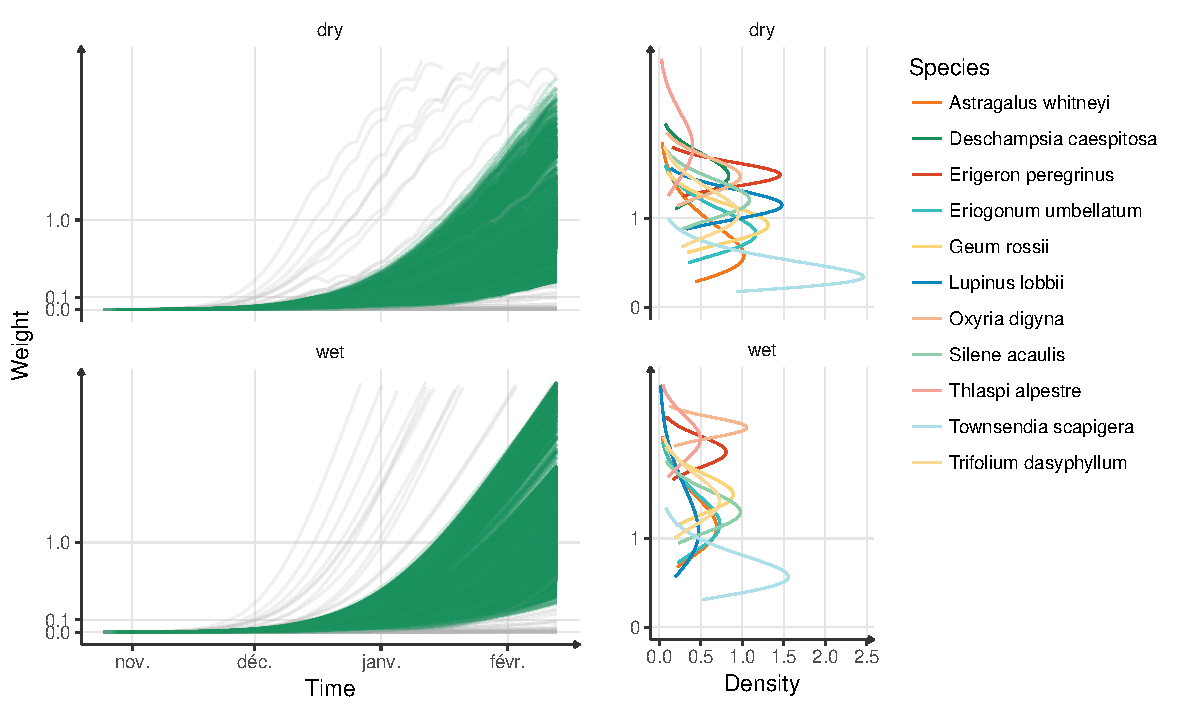
\includegraphics[width = \textwidth]{./2_PP/Figures/Calibration/weight_full_sim.pdf}
\caption{Comparison of simulated weights with distribution of weights of real alpine species for contrasting conditions.}
\end{figure}

\paragraph{Sensitivity analysis}
Relative importance of variables in the selection process is investigated with the packages \texttt{randomForest}. A random forest analysis (depth = 5, number of trees = 300) is performed on a balance dataset composed by all selected parameter sets and a random sample of rejected sets of equal size. Importance is assessed on the results of the random forest.

\subsection{Results}

\paragraph{Selection rate}
Parameter filtering process resulted in the selection of a low number of parameter sets (below 0.2\%) for each allocation algorithms (table \ref{table:selection_rate}). This number is below the sum of accepted parameter sets per species because a parameter set can match to multiple species. Not all species contribute to the same extend to the filtering process. \textit{Astragalus whitneyi} accounts for a high percentage of accepted parameter sets, while no parameter set could match 2 species (\textit{Oxyria dignya} and \textit{Deschampsia caespitosa}). The former is characterised by wide distribution in both conditions for the two variables of interest (weight and RSR), while the latter show relatively tight distribution with little overlap between the conditions for the both variables (see figure \ref{fig:comparison_BM} for comparison between simulations and data for total weight).

% latex table generated in R 3.2.3 by xtable 1.8-2 package
% Wed Nov 15 13:39:16 2017
\begin{table2*}\label{table:selection_rate}
\caption{Acceptance rate per species for the 3 main allocation algorithms. Because some parameter sets match multiple species, the total number and rate of accepted parameter sets is lower than the sum of accepted parameter sets per species. All rates are given in \%. }
%\centering
\begin{tabular}{lrr|rr|rr}
 & & non plastic & & fixed-eq & & plastic \\
  \hline
 species & n (2M) & rate & n (2M) & rate & n (200,000) & rate \\
% species & n (995603) & rate (\%) & n (995539) & rate & n (199964) & rate \\ 
  \hline
 Silene acaulis & 227 & 0.02 & 396 & 0.04 & 55 & 0.03 \\ 
 Trifolium dasyphyllum & 271 & 0.03 &  317 & 0.03 & 45 & 0.02\\ 
 Geum rossii & 51 & 0.01 & 72 & 0.01 & 12 & 0.01\\ 
 Thlaspi alpestre & 342 & 0.03 & 360 & 0.04 & 59 & 0.03\\ 
 Deschampsia caespitosa & - & - & - & - & - & -\\ 
 Eriogonum umbellatum & 500 & 0.05 & 805 & 0.08 & 118 & 0.06\\ 
 Townsendia scapigera & 593 & 0.06 & 930 & 0.09 & 107 & 0.05\\ 
 Astragalus whitneyi & 1570 & 0.016 & 2424 & 0.24 & 318 & 0.16\\ 
 Lupinus lobbii & 678 & 0.07 &  868 & 0.09 & 123 & 0.06\\ 
 Erigeron peregrinus & 1 & <0.01 & - & - & - \\ 
 Oxyria digyna & - & - & - & - & - & - \\ 
  \hline
  Total & 4233 & 0.43 & 6172 & 0.62 & 837 & 0.42\\
  \hline
 \textbf{Accepted} & 924 & 0.\textbf{09} & 1416 & \textbf{0.14} & 200 & \textbf{0.10}\\
\end{tabular}\end{table2*}

Despite the low selection rate, a difference can be noted between the \textit{fixed-equilibrium} algorithm and the two other algorithms with a accepted rate of 0.14 \% against 0.09\% and 0.10\% (table \ref{table:selection_rate}). This difference cannot be explained by a significantly better selection rate for specific species, but rather higher rates for all species.

Most of parameter sets are not shared between the algorithms (\textit{i.e.} around respectively and third and a quarter of accepted parameter sets are shared between \textit{non plastic} allocation and \textit{fixed-equilibrium} allocation calibrations), despite that the distribution of parameter values that are not shared are very similar and do not show any clear pattern (data not shown).

Out of the 31 parameters, 6 show graphical response of selection rate (see figure \ref{fig:accept_rate}), and only  \texttt{u\_max} and \texttt{P\_max} present a possible optimum different from limit values. The relative importance of the parameters is better explored in sensitivity analysis.



%Calibration filtering results in the selection of n parameter sets over m preselected parameters sets. Accepted sets are distributed among the 11 species of the dataset like presented in the table. Species A, B and C are the most numerous.\\


%Plasticity does not change the acceptance rate in any form (only slight increased from 0.26\% to 0.38\%, up to 0.42\% for full plastic). \\


\begin{figure}[p]\label{fig:accept_rate}
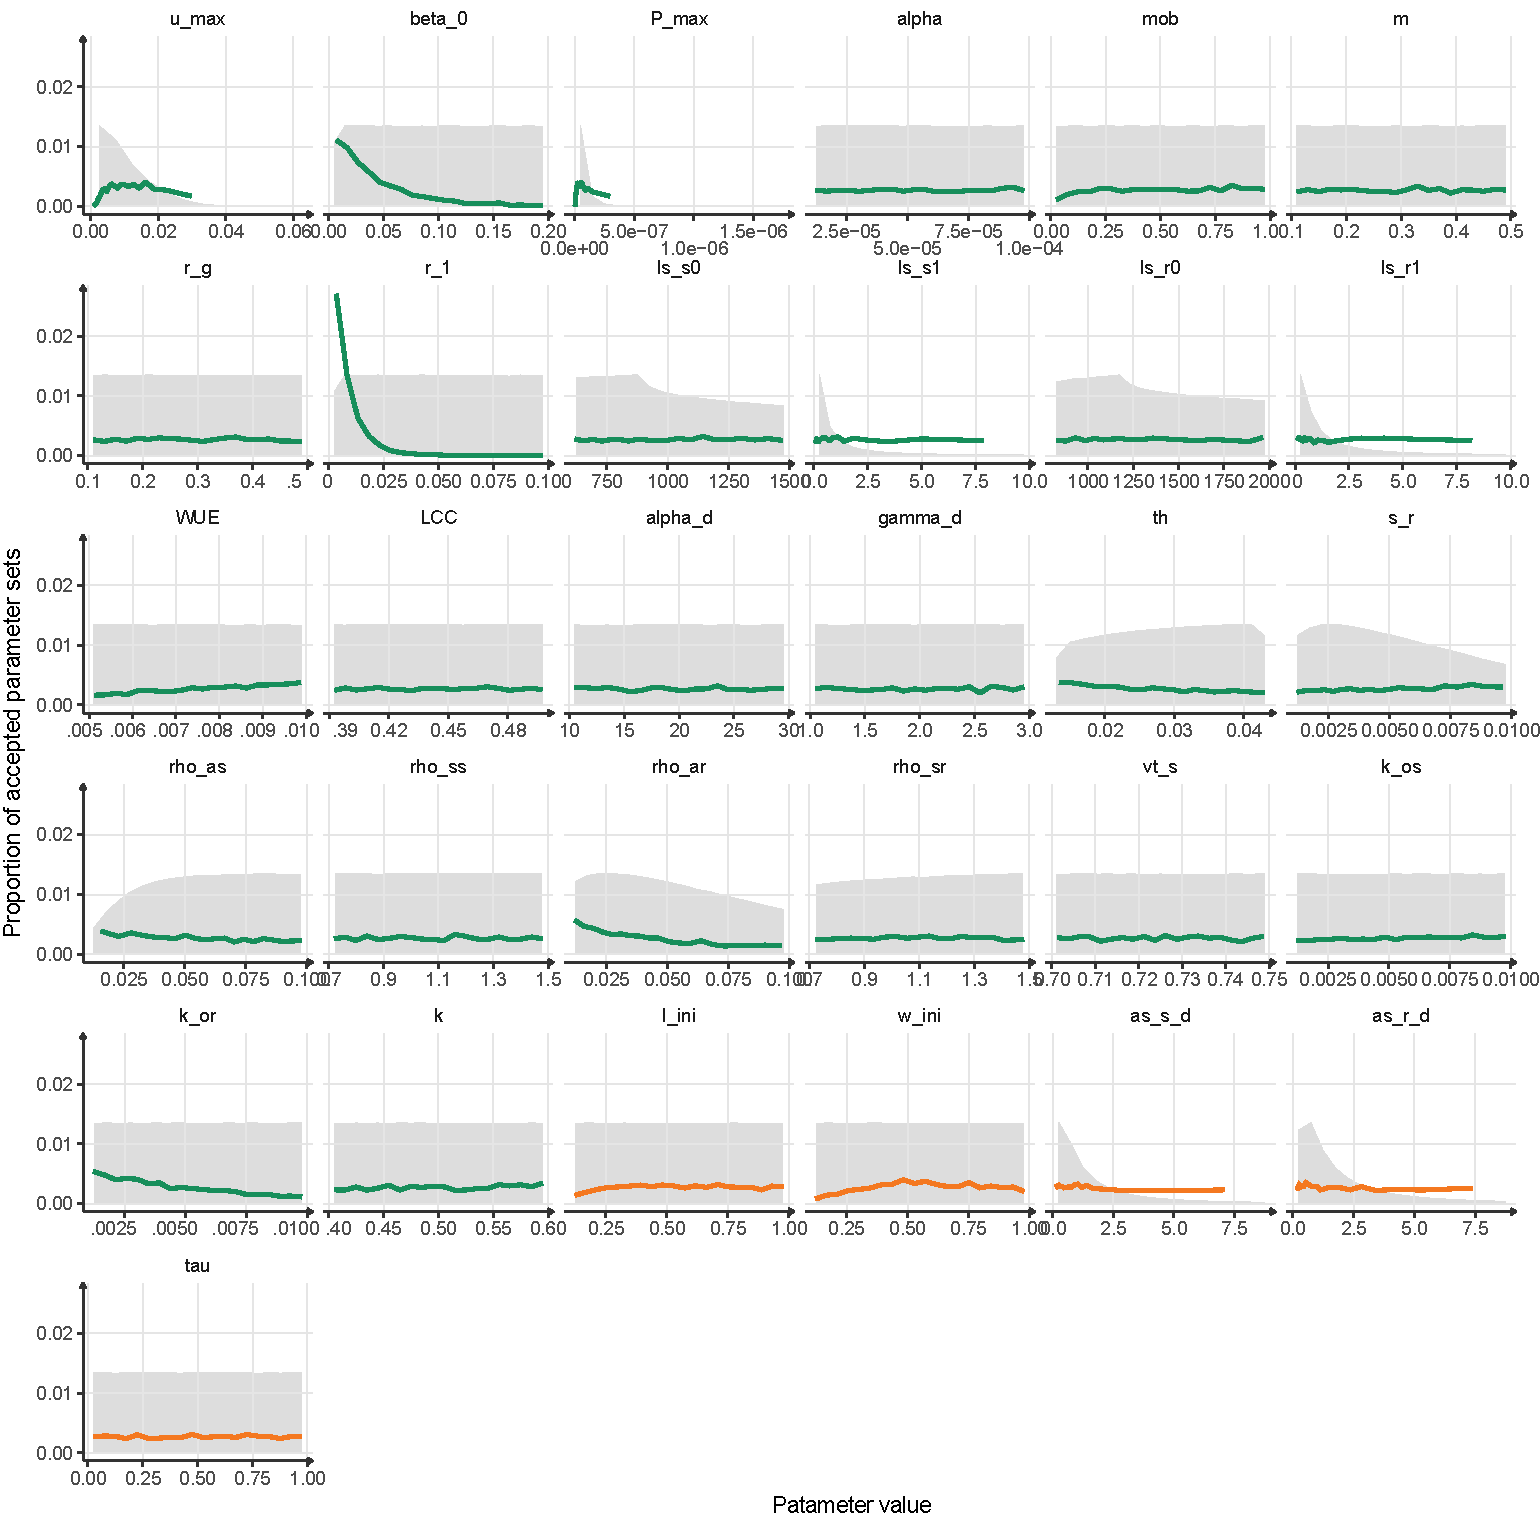
\includegraphics[width = \textwidth]{./2_PP/Figures/Calibration/acceptance_rate_RSRnWeight_per_par_none.pdf}
\caption{Selection rate per parameter for individual growth. \textit{Non plastic}.}
\end{figure}


%\begin{figure}
%%\includegraphics[width = 10cm]{/mnt/quadri1/simulations/exploration/species_par_space2017-11-06/plots/var_imp_plot_eq_design.pdf}
%\caption{Importance of the random forest to explain filtering outcome (accepted or rejected) of a balanced sample of parameter set between all tested (all accepted parameters and an equivalent sample in rejected parameters).  Fixed-equilibrium.}
%\end{figure}

\paragraph{Sensitivity analysis}


A total of 12 parameters show relative influence on selection rate for at least one of the algorithm. These parameters are divided between model parameters and species parameters. Species parameters show influence only for the \textit{non plastic}allocation algorithm. Model parameters express relatively similar importance for all three algorithms. The respiration rate of active tissues (\texttt{r\_1}) is the most sensitive parameters (see figures \ref{fig:accept_rate} and \ref{fig:importance}). Other sensitive parameters are related to water availability (\texttt{beta\_0}), organ exchange rates (\texttt{P\_max} and \texttt{u\_max}) and soil coverage by roots (\texttt{rho\_ ar} and \texttt{k\_or}).

\begin{marginfigure}\label{fig:importance}
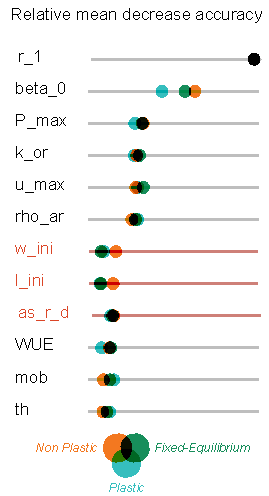
\includegraphics[width = \textwidth]{./2_PP/Figures/Calibration/importance.pdf}
\caption[Relative importance of main parameters for selection]{Relative importance of main parameters for selection under the three main allocation algorithms: (\textcolor{myOrange}{non plastic}, \textcolor{myGreen}{fixed-equilibrium} \& \textcolor{myBlue}{plastic}).}
\end{marginfigure}


%\begin{figure}[!h]
%   \begin{floatrow}
%\ffigbox{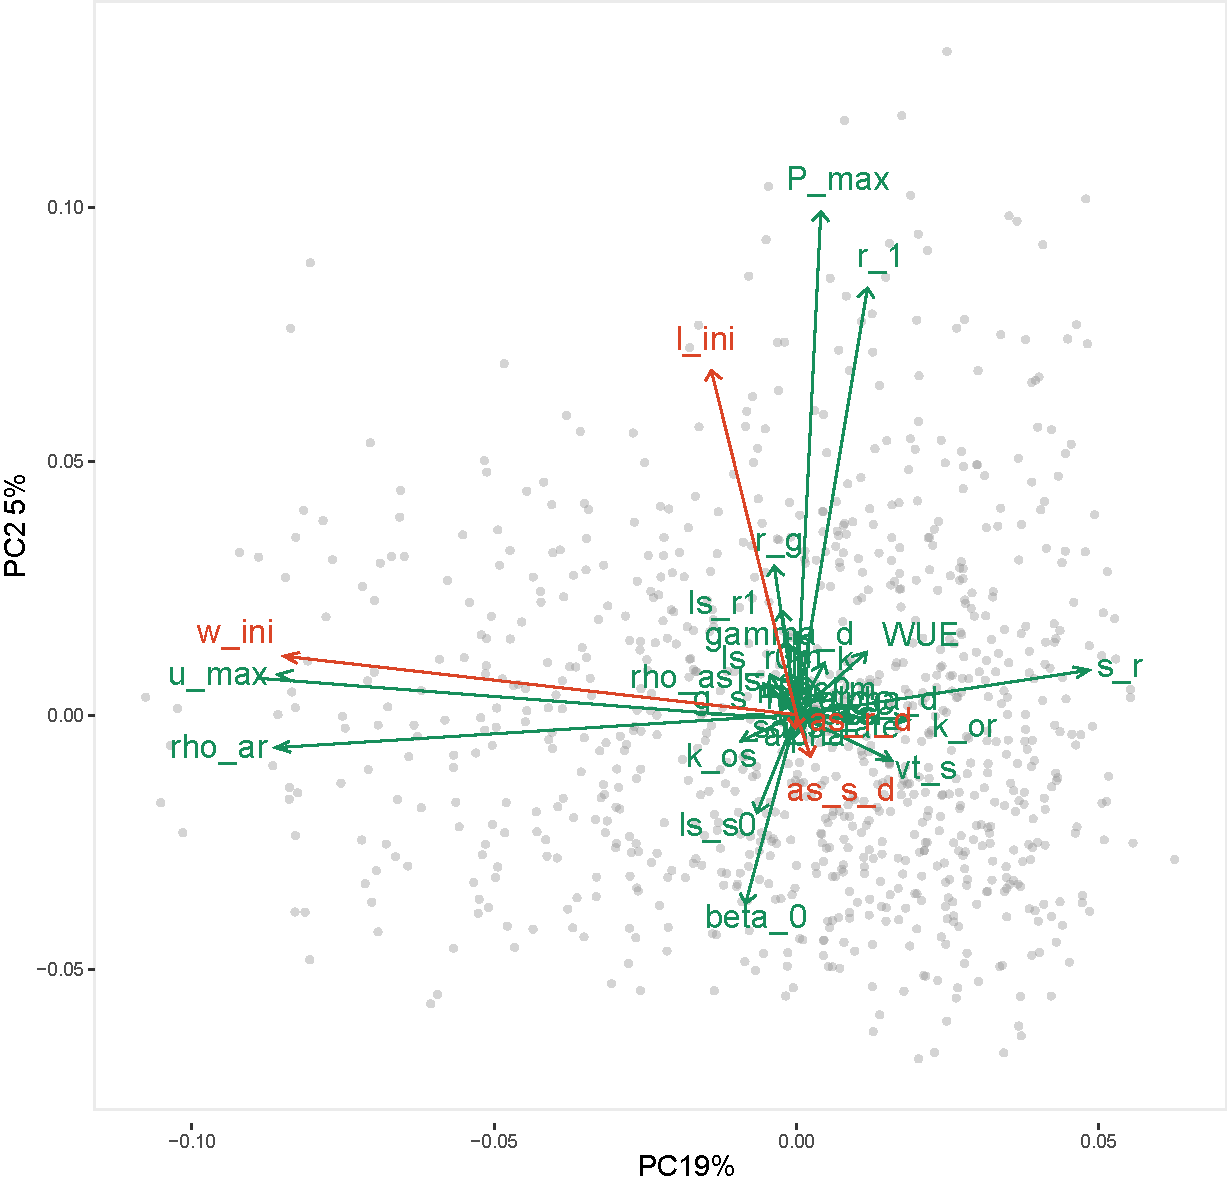
\includegraphics[width=\linewidth]{./2_PP/Figures/Calibration/PCA_none.pdf}}%
%\caption{First two axis of PCA of parameter sets selected in parameter filtering process. \textit{Non plastic}.}\label{fig:PCA_calibration}
%%       {\caption{second figure}\label{fig:example-2}}
%   \end{floatrow}
%\end{figure}
%\lipsum[3]

\begin{figure}%[tb]
    \classiccaptionstyle
\sidebysidecaption{0.60\textwidth}{0.3\textwidth}{%
    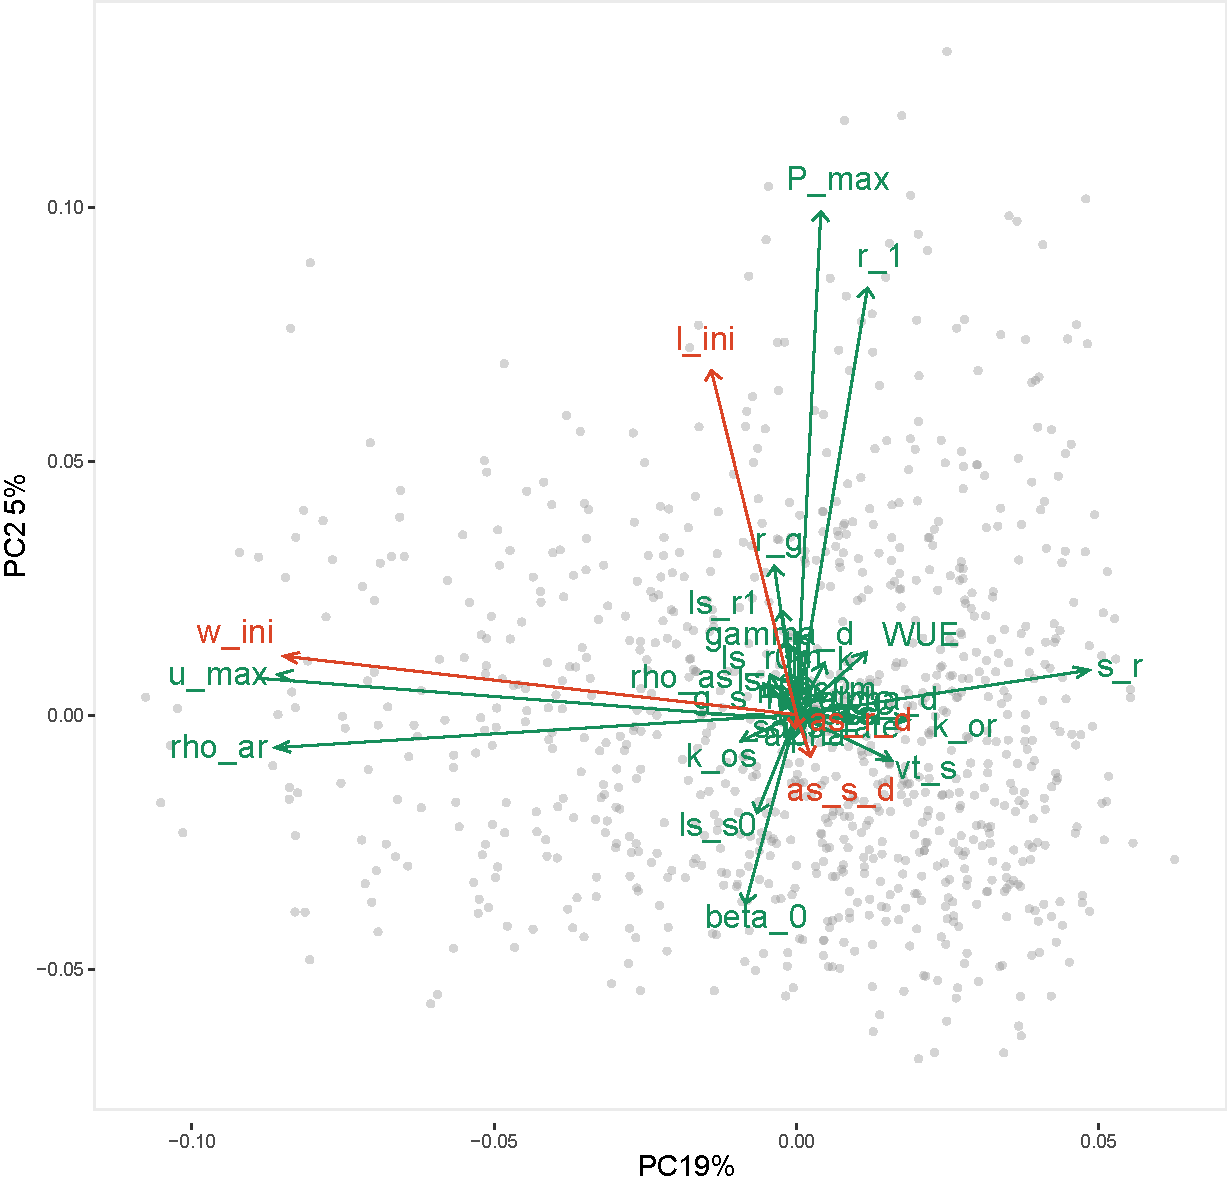
\includegraphics[width=1\linewidth]{./2_PP/Figures/Calibration/PCA_none.pdf}%
}{%
  \caption[PCA calibration]{Representation of the PCA of parameter sets selected in parameter filtering process on the first principal components. \textit{Non plastic}.}
  \label{fg:PCA_calibration}
  }
\end{figure}

The PCA performed for \textit{non plastic} algorithm only on parameter values reveals that important parameters are also the dominant variables that shapes the selected subspace. The two first axis explain only 14\% of variance. The first one is related to the root activity and efficiency (\texttt{u\_max}, \texttt{l\_ini}, \texttt{rho\_ar} and \texttt{s\_r}), the second is in line with global efficiency and resource availability.

The parameter filtering process is based on individual species, ... Species cannot be distinguished on these two main component space, neither on species specific parameters space (\texttt{l\_ini}, \texttt{w\_ini}, \texttt{w\_ini} \& \texttt{l\_ini}, \texttt{as\_s\_d}, \texttt{as\_r\_d}, \texttt{as\_r\_d} \& \texttt{as\_s\_d}) despite small variations in distribution shapes and ranges between species (data not shown).\\

\paragraph{Variable responses}
% Response of the two main vairables to main parameters.
For each algorithm the response of the two filtering variables (weight and RSR) are plotted against the most important variables in figures \ref{fig:sensitivity_BM} and \ref{ fig:sensitivity_BM}.

% Biomass
Total biomass is particularly sensitive to tissue respiration cost (\texttt{r\_1)}, but also maximum exchange rate parameters. There is a notable difference in growth maxima between the two conditions in favour of wet conditions, in line with observed data. This difference is observed for the three algorithm that differ mainly by the amplitude of the biomass ranges (need data).  Growth response curves are similar for all allocation algorithm. Growth is only weakly related to species specific parameters. Total biomass under \textit{Plastic-optimisation} algorithm seems to be more sensitive to variables influencing the exchange area per unit of biomass.

The species specific parameters \texttt{tau} controlling the balance between genetic and environmental control does not emerge as a influencing parameter at the global scale for any of the two flexible allocation rules.

\begin{figure}\label{fig:sensitivity_BM}
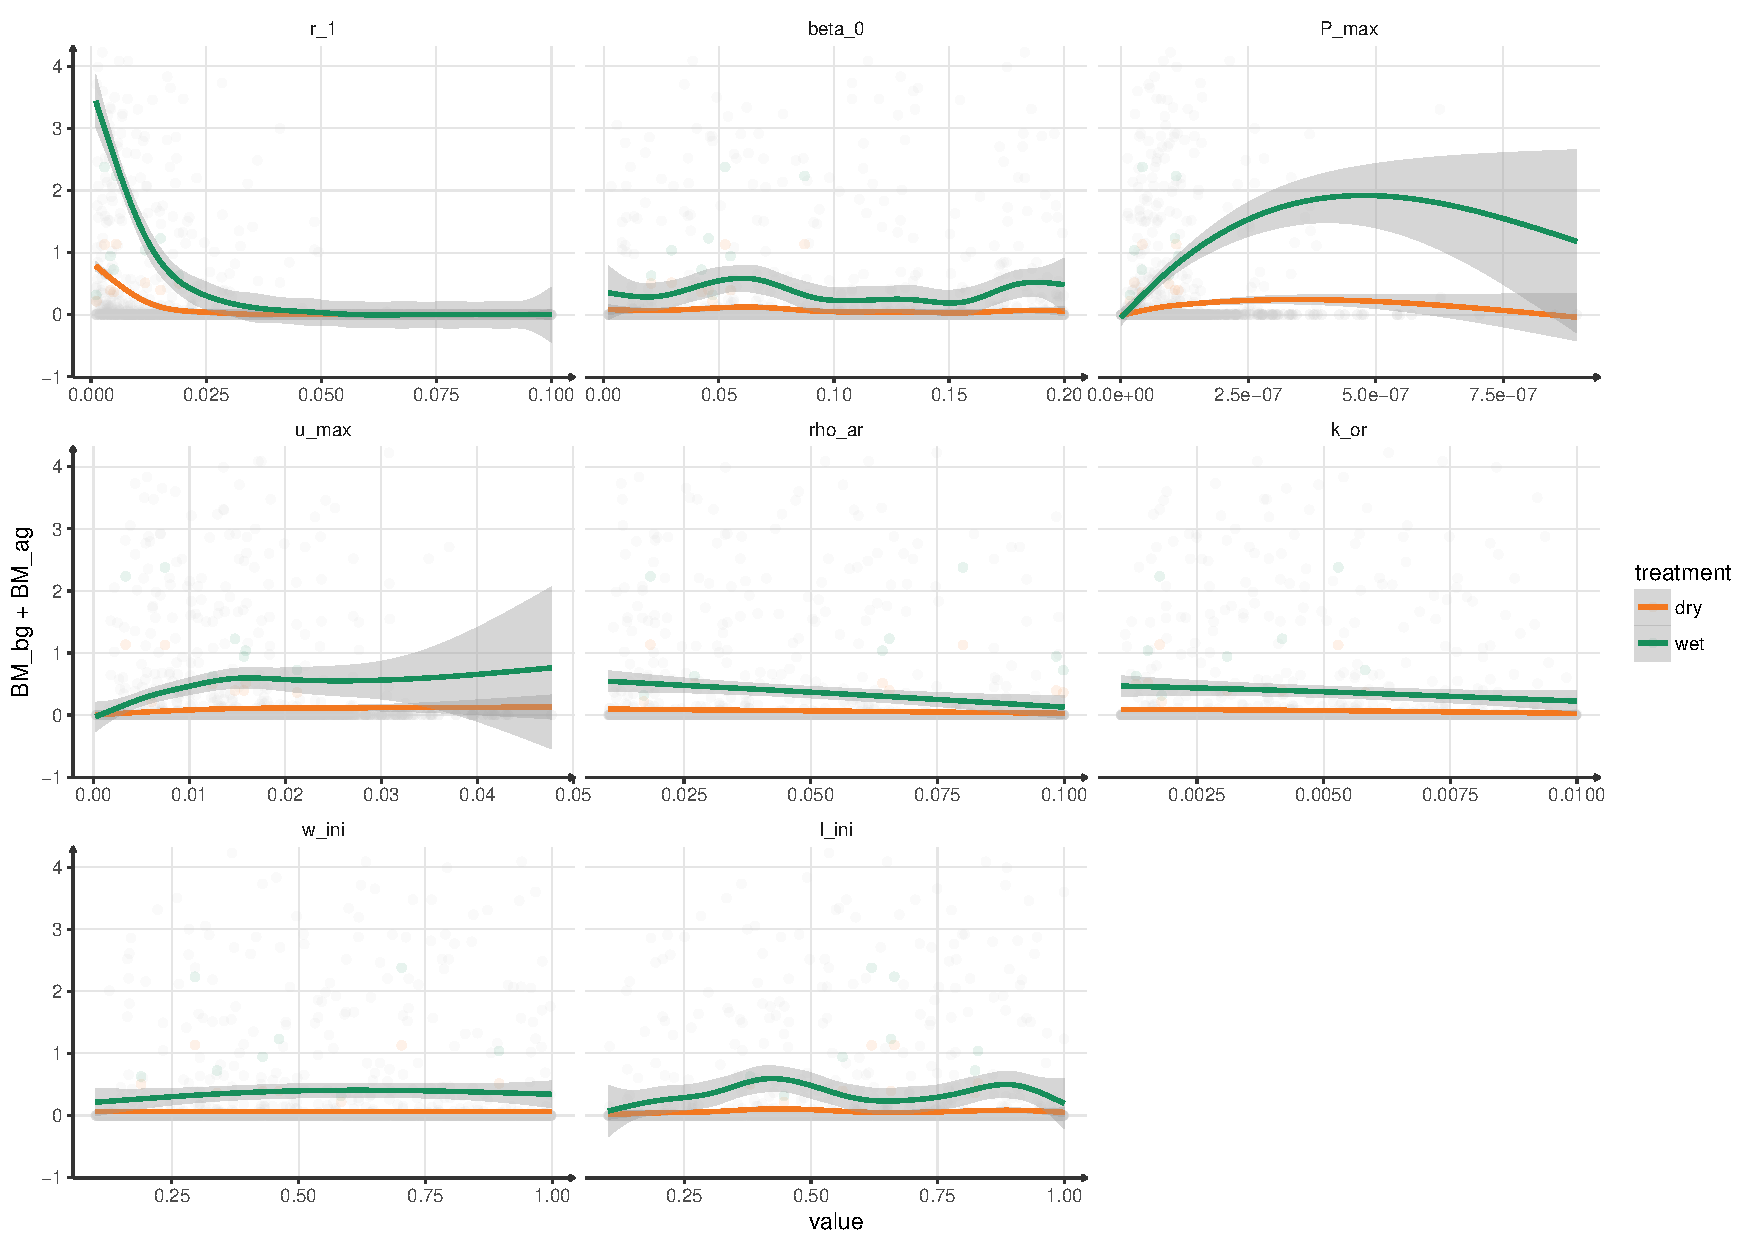
\includegraphics[width = \textwidth]{./2_PP/Figures/Calibration/par_effect_none_BM.pdf}
\caption{Main parameters effect on the total plant biomass. \textit{Non plastic}. One dot represents a parameter set. Not all parameter set are represented as the y axis is limited around the smooth function (loess). Coloured points represent selected parameter sets in the two treatments (\textcolor{myOrange}{dry} and \textcolor{myGreen}{wet}).}
\end{figure}

% RSR
Root:Shoot Ratio (or RMF in figure \ref{fig:sensitivity_RSR}) strongly responds to species specific parameters under \textit{non plastic} allocation because the memory parameters(\texttt{l\_ini} and \texttt{w\_ini}) are the means plants control their RSR. For other allocation rules, species specific parameters have little control over RSR. Surprisingly, the photosynthetic capacity has stronger influence on the ratio than the root maximum exchange rate.


\begin{figure}\label{fig:sensitivity_RSR}
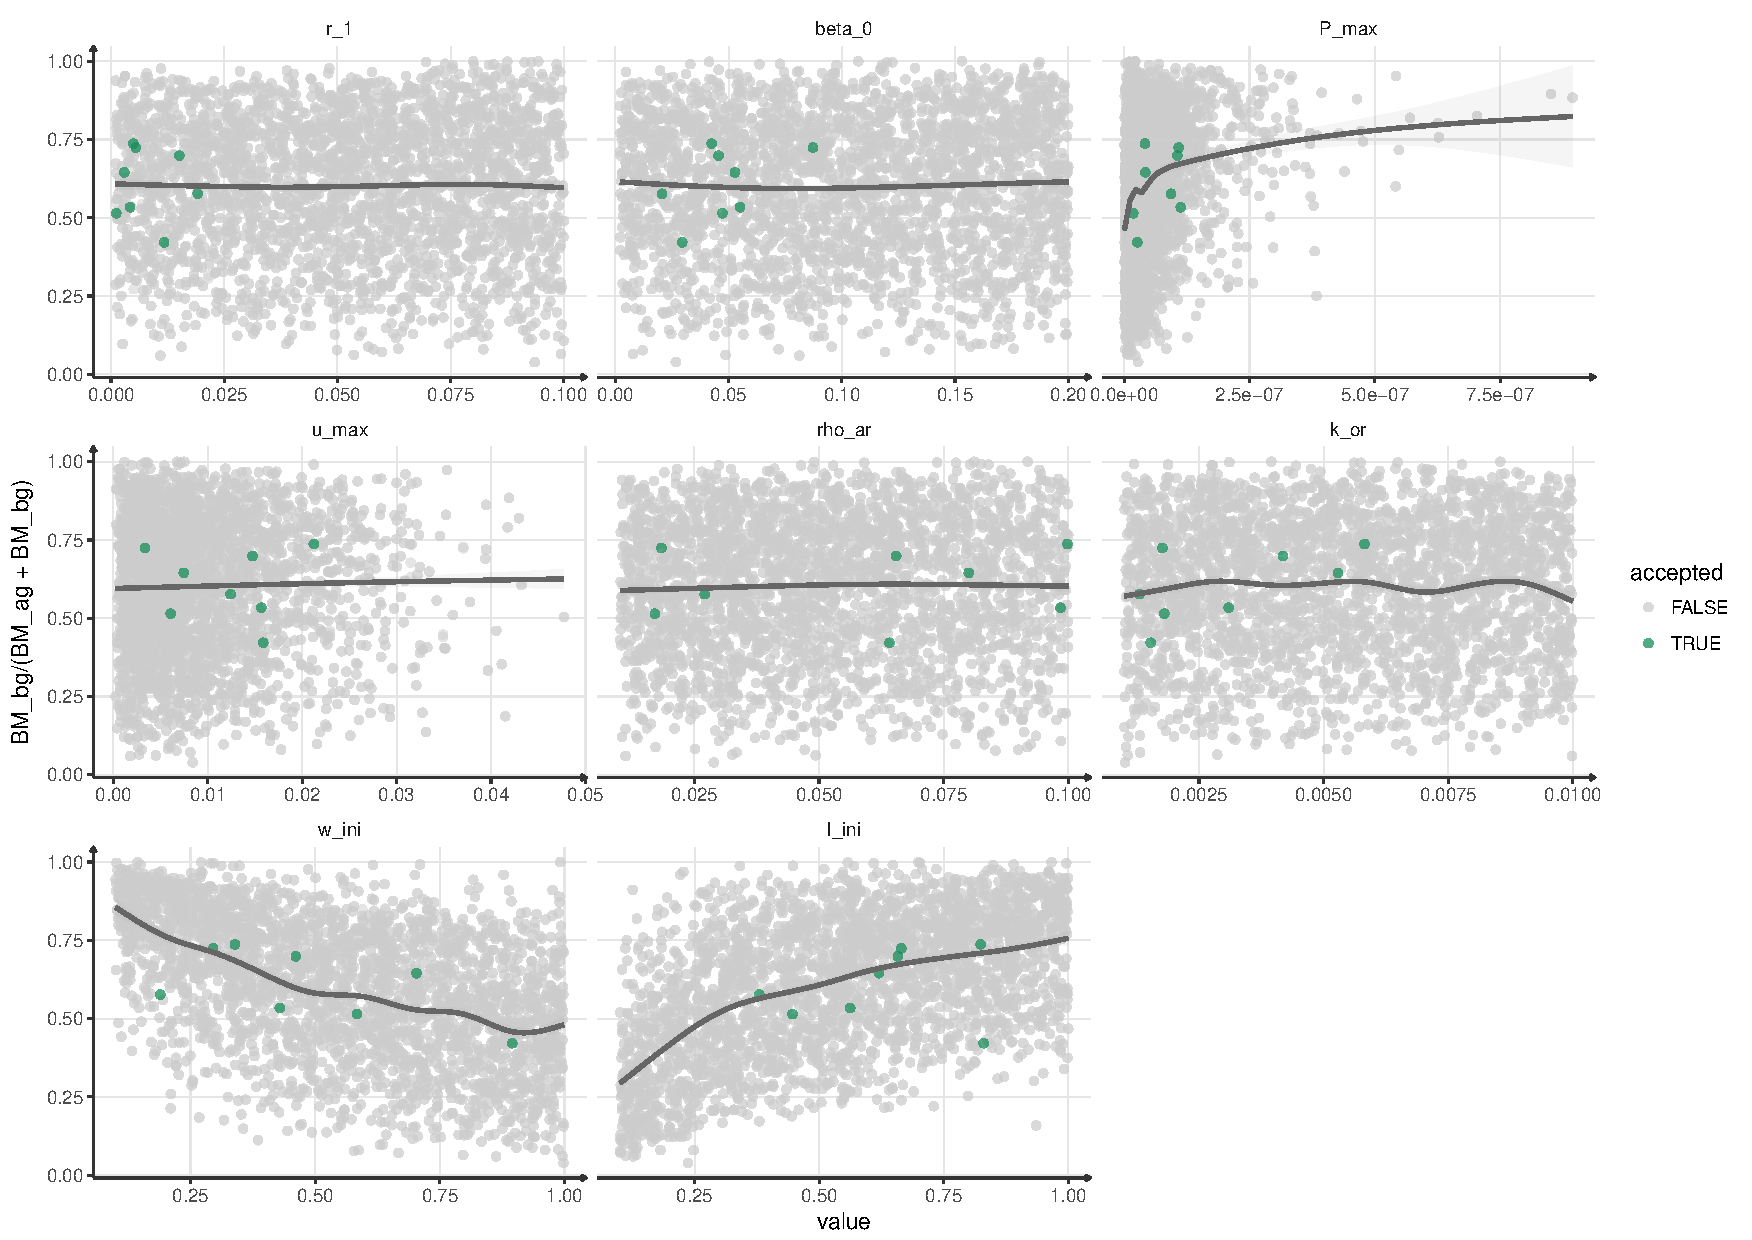
\includegraphics[width = \textwidth]{./2_PP/Figures/Calibration/par_effect_none_RSR.pdf}
\caption{Main parameters effect on the total plant Root Mass Fraction (RMF). \textit{Non plastic}}
\end{figure}

% TAU

\paragraph{Root shoot ratio and plasticity}

Little to no difference in RSR is expected for \textit{non plastic} allocation rule since allocation promoted a fixed phenotype, but both \textit{fixed-equilibrium} and \textit{plastic-optimisation} allocation rules allow for changes in RSR. Nevertheless, no stable change in RSR is observed in any of the simulations. Fluctuations are present but consist in stable oscillations between two fixed values (see figure \ref{fig:comparison_RSR}), synchronized with water variations. These rapid adaptations of the relative proportion of roots denote a high flexibility of plant phenotypes in \model.


\begin{figure}\label{fig:comparison_RSR}
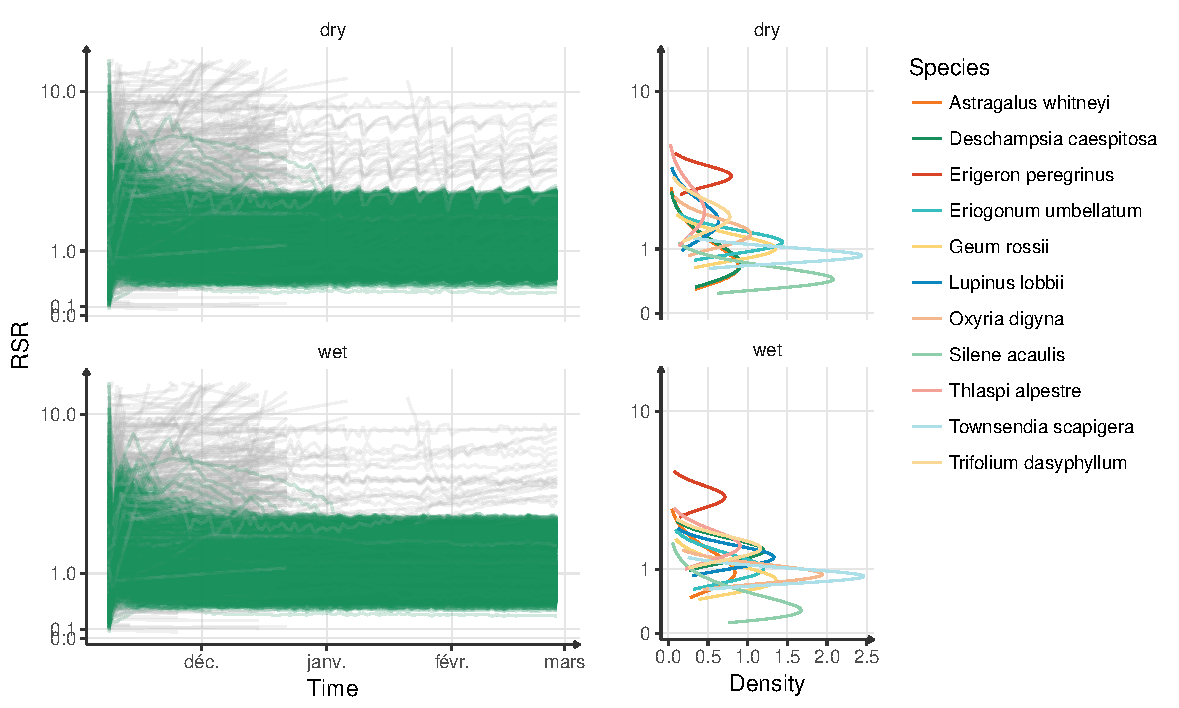
\includegraphics[width = \textwidth]{./2_PP/Figures/Calibration/RSR_full_sim_f-e.pdf}
\caption{Comparison of simulated values of RSR with real species RSR in two contrasting conditons. Because there is no plasticity or ontogeny, the simulated plant do not express any chagnes in RSR. \textit{Fixed-equilibrium}.}
\end{figure}

\subsection{Discussion}

\paragraph{Growth and strategy space}

The relative low selection rates for all allocation rules highlight the complexity of fitting such complex model to empirical data, despite the relative simplicity of the data. This difficulty seems to lie in two factors: the high number of parameters and the lack of stable changes in RSR. This last point is further discussed in the following paragraphs. Nevertheless, plant growth is reproduced in two contrasting conditions for multiple species, and while plastic algorithms have a greater potential for growth (more high growth rate), this is not systematic and the absence of clear pattern for the most influencing parameters, such as maximum exchange rates and respiration rates, indicates that such high growth depends on a combination of parameter values. I believe that the shape of gain and cost functions along the functional trade-off between active and structural tissues plays a determining role in the growth. A trade-off function with a wider viable range is more likely to be selected as more strategies would grow (therefore reducing the relative sensitivity to species-specific parameters). Considering the exponential shape of the turn-over function (one of the main cost with respiration), the width and height of the trade-off (or net gain function) is probably more strongly linked to the gain functions (exchange rates) and linear cost function (respiration), explaining little effect of parameters related to lifespan (already preselected otherwise). There is a strong dependency between viable strategies (and as a consequence functional potential diversity) and the main trade-off between resource acquisition and efficiency.

Filtering the parameter sets based on all species instead of individually would have been ideal to quantify this link and better calibrate the model. However, such approach would have required many more simulations, when the parameter filtering method was chosen for its low computational cost. Moreover, considering the number of species-specific parameters, fitting the strategy subspace (at least default active tissue allocation parameters, the memory of resources and stability) of 11 species to the data in combination with more than 20 models parameters is near impossible. Ones should have had first determined the relative positions of the species within the said strategy space before any global calibration routine. Nonetheless, species-specific parameters have an influence on model main variables. Memory parameter affected the RSR in the context of \textit{non plastic} allocation rule (see figures \ref{fig:comparison_RSR} and \ref{ fig:importance}, while the default proportion of active tissues in roots was an influencing parameter in all algorithms (figure \ref{fig:importance}, \texttt{as\_r\_d}). Therefore, they should be analysed in further simulations within the same set of model parameters.

Because of the model complexity and the number of species specific parameters, in addition to long simulation time, Bayesian calibration could not be performed. In the Bayesian paradigm the information is contained in the data and revealed by the structure of the model. An alternative modelling approach is to used the parametrisation phase to accept certain parameter sets, and learn about the system through simulation experiments. The simulated data is analysed rather than empirical data. The patterns emerging from the simulation experiments inform us on the impact of the modelled mechanisms (even if they do not totally match the data). Therefore the model is still an understanding tool and can inform the effect of plasticity on ecological processes.\\


\textbf{The growth is reproduced in contrasted conditions, but only partially as one per parameter set is tested. The number of species and dimensions in the strategy space would not allow for a calibration of all species for one parameter set. The plastic response of the root:shoot ratio is not correctly reproduced and would require a different implementation (stress based). However the plasticity as implemented improved the acceptance rate because of a better growth. Therefore the effects of plasticity can still be investigated with simulation experiments.}

\paragraph{The role of water}

If the parameter filtering step did not result in the selection of optimum values for all parameters, it provides information on the main mechanisms influence plant growth. 
Indeed, the relatively high importance of parameters related to water shows the importance of the resource on the model behaviour. Both water availability (water absorption limitation, exchange rate) and root mass and construction parameters are important to match the empirical data. Considering that the calibration relies on experiment data of drought events, it is no surprise that parameters related to water economy show strong influence on the selection rate and model behaviour. In the context where the model has been developed, water shortage is expected to an important factor in community dynamics. In this perspective, the ability of \model to reproduce the difference in productivity in both conditions, and the relative sensitivity to water related parameters is an advantage. The link between water resource, species strategy, plant performance and phenotypic plasticity is explored more in details in the following section.


%Differences between algorithms that make sense: more biomass, sensitive parameters are related to how plasticity work...

\textbf{The sensitivity of the different variables to the parameters align with the two criterion of selection (that work with the independence of trade-off). In contrast with forest, the light is not the most important factor and water plays a more limiting role. A particular focus on below-ground resources should drive the simulation experiments with this model.}

\paragraph{More complex plasticity?}

As mentioned earlier in this discussion, the model is not able to produce any shift in RSR in different water treatment. It is not a surprise for \textit{non plastic} algorithm, but the filter was still applied on this criterion to allow the comparison with plastic algorithm and to be able to measure the improvement in selection rate. However, even plastic algorithms do not show strong enough response to water treatment in term of RSR. A strong and good (in the sense it would have matched the data) is larger in amplitude and more stable in time. Such processes generally amplify with time, \textit{i.e.} when the number of drought event increases, the response (allocation to roots) increases (relative to default phenotype). Unlike natural systems, plants in \model fluctuates between two "states", or phenotypes associates to the dry and wet conditions. The RSR post drought event is reached after the first week without water. This can be explained by two main mechanisms that are related but have contrasting implications. The quickness in response to the changing conditions is allowed by relatively high assimilation rate. If the net growth rate is controlled by the total weight condition during the filtering process, the assimilation rate is not and can be compensated with relatively high turn-over rate. Net growth rate being equal, species with higher assimilation rate will have higher phenotypic flexibility (higher fraction of biomass to invest in carbon pool of choice) than species with lower assimilation rate. This flexibility, similar to reallocation, allows changes in RSR, but not the accumulation of biomass in roots. Unfortunately, both the constant turn-over rate implemented in the model, and the selection toward "wide and high" gain functions limit control on this aspect.

Moreover, the fact that plants are more productive during periods where they may not want to invest in roots strengthen this effect. Indeed, a plant would drift to higher RSR if it was more productive when pursuing the high RSR phenotype than when pursuing the low RSR phenotype. This last point mentions the "will" of the plant, in the context of \model this target phenotype is encoded in the projection of external conditions. Because this projection is daily based by design, the accumulation of drought stress is not translated in the internal projection variables of the plant (like it can be with the accumulation of phyto-hormones.). This limitation highlights a big difference between simulated plants in \model and natural plants. While solutions to overcome this problem can easily be imagined(see equation \ref{eq:projection_alt} in \ref{subsection:submodels}), they would require more parameters and introduce more complexity to the analysis. This model provides a first approach to phenotypic plasticity in grassland models and the formulation of the projection, key element of the phenotypic plasticity, is certainly a starting point for further development. Nevertheless, the differences in response to the parameters between the three allocation rules, despite shared plant functioning, demonstrate the importance of plasticity itself. And simplification of the processes should not be a reason to not explore its effects. The fact that the parameter \texttt{tau} has a relatively small impact on selection rates alos support the need to better understand all strategic axis before focusing on the effect of projection. While there are many ways of simulating the phenotypic plasticity, the parsimony is privileged. This simple representation is enough to understand the effects of active plastic allocation in association with the other strategic differences between species.


%Exchange area per biomass and sensitivity to exchange rates : trade-off are important and structuring.

%filtering on RSR to test if plasticity improved selection of parameters, = is an essential part of platn functioning.\\
%\paragraph{Modelling paradigm}
%Bayesian paradigm where the information is contained in data and revealed by the structure of the model. Go for simulation experiment approaches where the model is used as a simulation tool and results as new data. The emerging patterns inform us on the impact of the modelled mechanisms (even if they do not totally match the data). Model as an understanding tool.\\
%While many ways of simulating the phenotypic plasticity can be proposed, the parsimony is privileged and this representation is enough to understand the impact of related processes shared by any representation of phenotypic plasticity is the developed framework.

%\textbf{Root shoot ratio changes were not captured by the model. The structure of the plasticity mechanisms does not work with the given watering cycle. Needs to add one parameter for reactivity.}



% ##################################################################################
\section{Individual level behaviour and properties of plastic allocation algorithm driven by the plant memory}


Calibration and sensitivity analysis give information on the main processes of plant growth, but the general effects of the allocation rules on plant growth are not fully identified. Moreover, because the parameter filtering processes was limited to individual plants and the effects of the species specific parameters are depending on the other parameters of the model, the effects of these species specific parameters should further be investigated. The objective of this part is to set better understanding on the role of the \textemph{allocation rules} and species \textemph{memory} on plant development as basis for interpretation of plasticity effects in following chapters.

The challenge of the framework presented in the paragraph \ref{subsection:memory} under \textit{plastic-optimisation} is to control the phenotype with the values of the memory. The risk of this approach is to have too tight estimation function of the fitness (or driving function) and to see the convergence of all species (with different memory values) toward the same phenotype (same allocation of active and structural tissues in roots and shoot). The extend to which different species memory lead to different phenotypes under full genetic control (not influenced by the external conditions) is explored through simulation experiment under \textit{plastic optimisation} allocation algorithm with no effect of conditions on traits ($\tau = 1$), only on growth.

%Proof of concept
\subsection{Method}


%\paragraph{Strategy diversity filtering}
%To further reduce the number of parameter sets considered, we proceeded in an additional filtering step. Because the first filtering was conduced for only one strategy over the whole 4D strategy space (l\_ini,  w\_ini, as\_s\_d, as\_r\_d) it is necessary to verify that other strategies do not lead to potential Darwinian demon. This should be limited by the choice of priors, while at the same time promoted by the selection of parameters increasing growth to counter balance potential unfitted strategies\footnote{Better do that beforehand than after... But I guess it's too late now.}.

\paragraph{Allocation algorithms}
The effect of allocation rule on phenotypic development is investigated thanks to pot simulations (see Methods in \ref{section:calibration}) of 100 days in 3 watering treatment: 2mm, 8m and 16mm per day. To avoid drift in the phenotype due to allocation algorithm (see paragraph \ref{subsection:memory} on phenotypic determination), simulations where run a first time, then rerun with default specific traits matching traits at the end of the first simulation set. All four algorithms are simulated. To reduce the number of simulations 100 parameter sets are selected randomly within the accepted parameter sets for the \textit{non plastic algorithm}.

\paragraph{Memory \& phenotype}
Memory of external conditions plays a determining role in phenotypic development under \textit{plastic-optimisation} allocation rules. The effect of the memory alone (environmental cues ignored by setting \texttt{tau} to 1) on the default emerging phenotype is explored for diverse memories (9 values on the two axis from 0.1 to 1 later scaled to the maximum area exchange rates for model parameter set considered, or 81 values) for each accepted parameter set. The effect of the memory values on the final position of plants in the phenotypic space are visualised by fitting loess curves between memory values and individual trait values.

\subsection{Results}

\paragraph{Allocation algorithms}

\begin{figure}\label{fig:allocation}
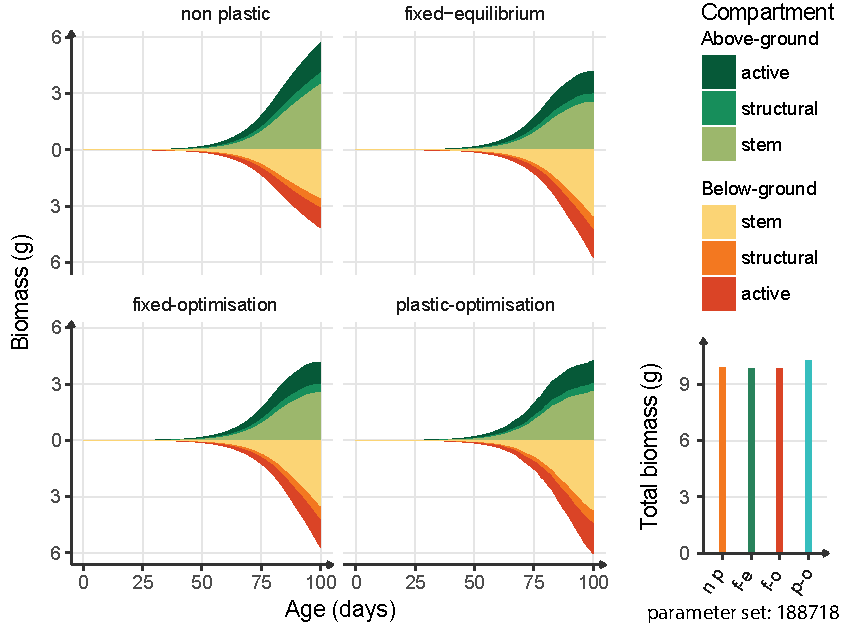
\includegraphics[width = \textwidth]{./2_PP/Figures/Individual/allocation_rules.pdf}
\caption[Effect of the different allocation algorithms on the different biomass compartments]{Effect of the different allocation algorithms on the different biomass compartments of the plant. The fraction of organic matter allocated to the stem (ensemble of supporting tissues for shoot and roots) are increasing over time for all algorithms. The \textit{non plastic} algorithm show constant allocation coefficients between above-ground and below-ground compartments and between active and structural tissues. All others show different coefficients for the above-ground - below-ground partitioning, and the \textit{plastic-optimisation} algorithm have changing proportion of active and structural tissues. The bottom-right panel show the total biomass for the four allocation algorithms after 100 days. }
\end{figure}


%think of a "showtime" visualisation that shows how growth and traits are impacted by allocation rules and \texttt{tau}.\\

The allocation algorithm affect the way the organic matter in distributed between the different tissues of the plant. With partitioning coefficient pre-established for the given conditions, the algorithm show very similar performances (see figure \ref{fig:allocation}). The difference in allocation algorithm is mostly noticeable in figure \ref{fig:allocation} mostly on the shift toward root allocation at the end of the simulation when the water becomes to be limiting. The plant under \textit{plastic-optimisation} allocation benefit from a light improvement in performance (mean: +10\%, median: +3.4\% relative to \textit{non plastic}).

The \textit{plastic-optimisation} algorithm allows changes in the proportion of active tissues in organs. This may have repercussions on the allocation between shoot and root, but also can lead to non specific variability within plants with no perception of resource fluctuations ($tau = 1$). The median variability of the RMF (root mass fraction) along the 100 simulated days is 0.015, that is five times higher than the variability of the other plastic algorithms (\textit{fixed-optimisation} and \textit{fixed-equilibrium})(see table \ref{table:variability-rmf}). This variability is much higher (around 0.028) for the plastic plants in all three plastic algorithm, while it is null for the \textit{non plastic} allocation rule. The range of the RMF follows similar trend, with higher value for the \textit{plasti-optimisation} than the other algorithms when plant do not perceive the resource fluctuations, and wide range for all plastic allocation algorithms when plants take into account the changes in light and water resources.

\begin{table}[h]
\centering
\caption{Median of variability and range of the RMF for simulations of 100 days, for 100 different parameter sets and three different water treatments (2, 4 and 8 mm per day), in the four different allocation algorithms. sd: standard deviation.}
\label{table:variability-rmf}
\begin{tabular}{l|ll|ll}
            & \multicolumn{2}{c}{\textbf{sd}}              & \multicolumn{2}{c}{\textbf{range}}           \\
\hline
\textbf{algorithm}                     & tau = 0          & tau = 1          & tau = 0          & tau = 1          \\
\hline
none                 & $<10^{-12}$ & $<10^{-12}$ & $<10^{-12}$ & $<10^{-12}$ \\
fixed-equilibrium    & 0.0278           & 0.00212          & 0.173            & 0.0155           \\
fixed-optimisation   & 0.0279           & 0.00221          & 0.173            & 0.0161           \\
plastic-optimisation & 0.0283           & 0.0150           & 0.174            & 0.0839          
\end{tabular}
\end{table}

The plastic algorithms show similar levels of variation and range, while the \textit{non plastic} one is stable as expected. The \textit{plastic-optimisation} allocation show more instability for non plastic plants ($tau = 1$) but that is lower than the variability observed in plastic plants ($tau = 0$). The allocation (and therefore phenotype) is controlled by the allocation rules (plastic dimensions and objective functions) and the estimation of conditions. Before investigating the effects of varying conditions, it is important to understand the effect of memory on plant strategy and phenotype.

%Have the proportion of tissues changing over time\\

%Show the respiration, assimilation and turn-over rates.\\ 

%Isn't it possible to show these along memory or active/str ratio axis ?


\begin{figure}\label{fig:plastic_allocation_trajectory}
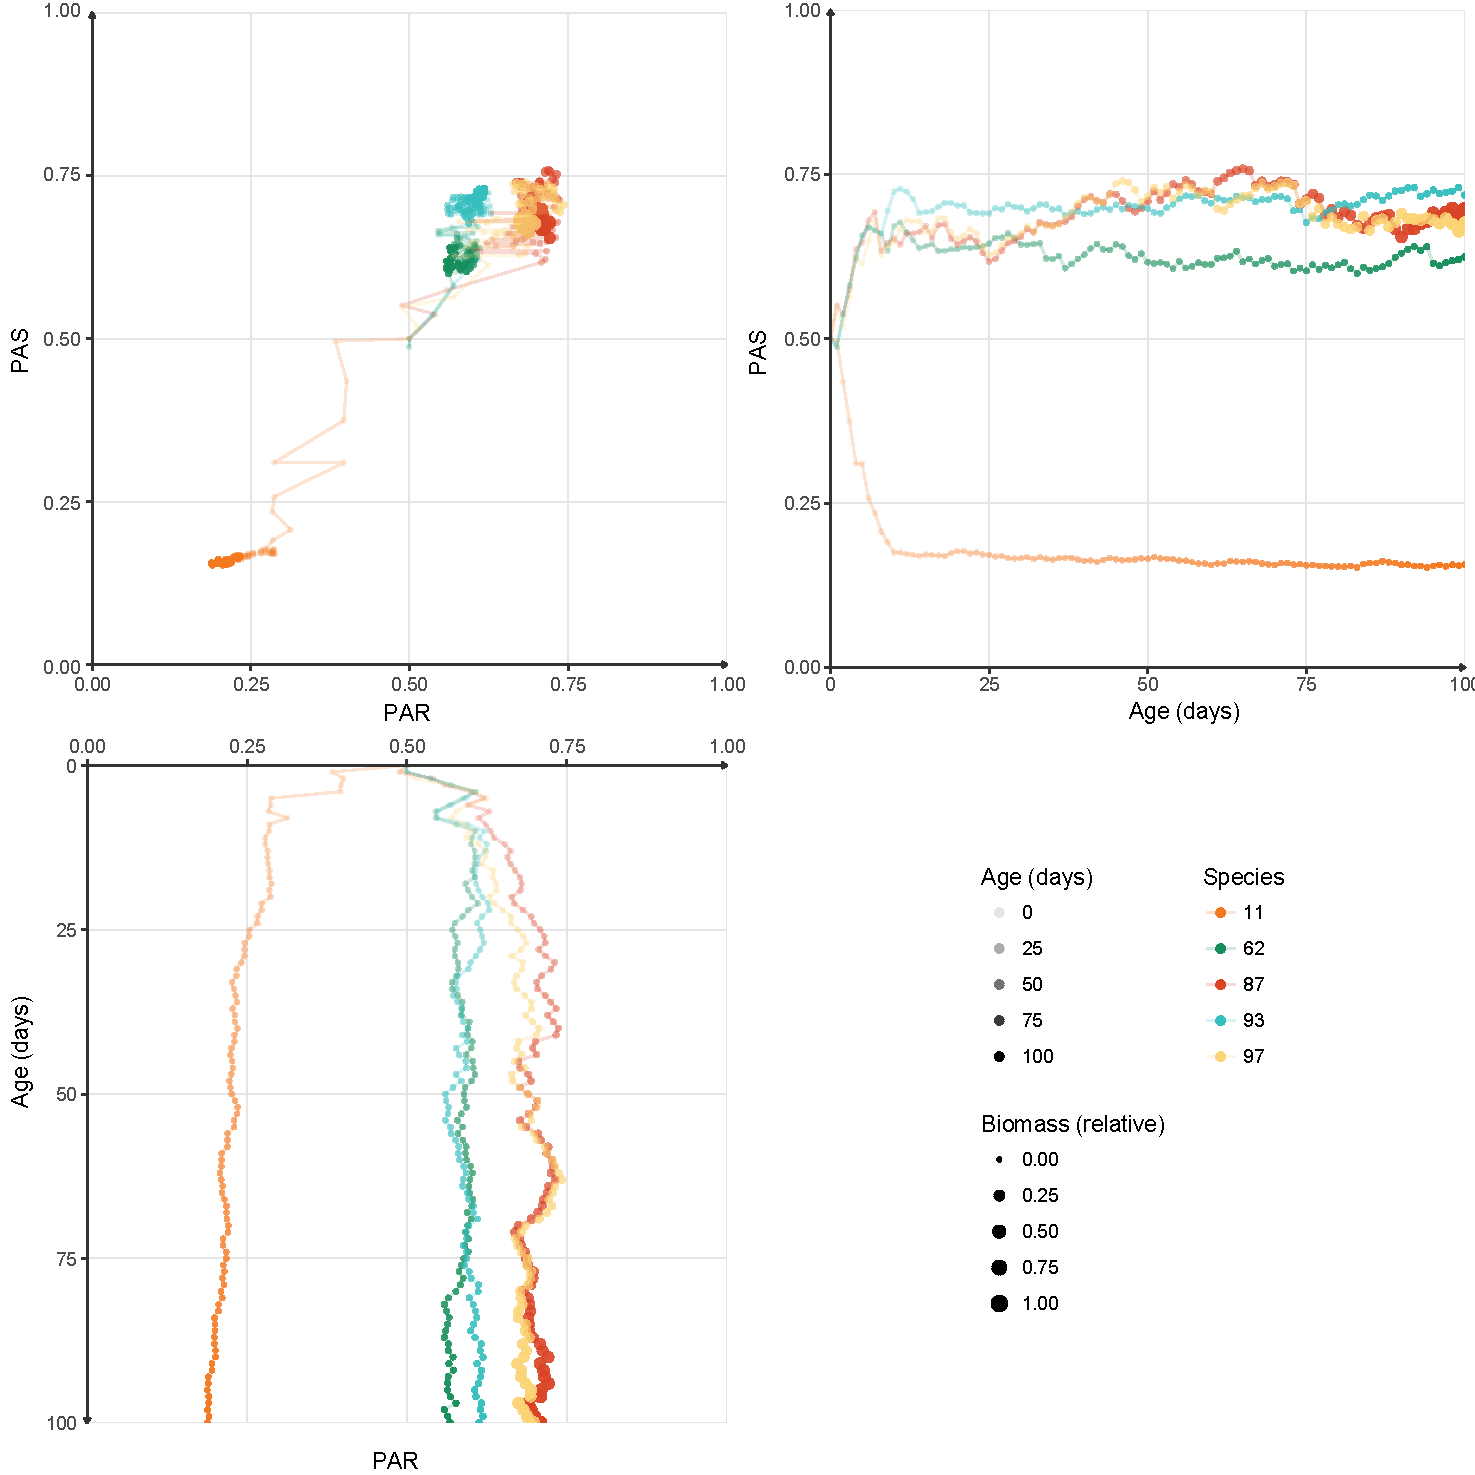
\includegraphics[width = \textwidth]{./2_PP/Figures/Individual/memory_effect.pdf}
\caption{Trajectories along time in the strategy space of 5 plants with different memories. After 10 days, all plants have converged toward the estimated optimum.}
\end{figure}

\paragraph{Memory and phenotype}

The kinetic of the phenotypic shift is first visualised for one parameter set on the two main phenotypic axis (proportion of active tissues in roots: PAR and proportion of active tissues in shoot: PAS). From the same starting point the five species show distinct rapid shift toward segregated subspace of the 2D strategy space. The equilibrium point is reached in approximately 10 days for all 5 species. Despite constant memory, variations are visible on both tissue allocation traits of roots and shoot. These variations lead to partial overlap but the five species are distinct on the 2D space.

The memory of resource availability is a strong enough driver to alter the default phenotype of a species. The effect of the two components of the memory (memory of water availability and memory of light availability) on the three main traits is explored through local regressions. The proportion of active tissues in roots increases to a plateau with increase in water availability memory (figure \ref{fig:w_ini_p_as_r}). This response pattern is consistent between all parameter sets, but the starting points and slopes may differ. The same pattern is observed between light availability memory and proportion of active tissues in roots (data not shown). The allocation convergence in the root is also influenced by the increase in light availability memory. An increase in the latter leads to a smooth increase in the former (see figure \ref{fig:l_ini_p_as_r}) with less drastic response than the water. This response is mirrored in shoot allocation response to increase in water availability memory (data not shown). Both organs react in symmetric ways to increases in resource availability. The RSR has a negative log response to water availability memory (positive in the case of light availability memory).

\begin{figure}\label{fig:w_ini_p_as_r}
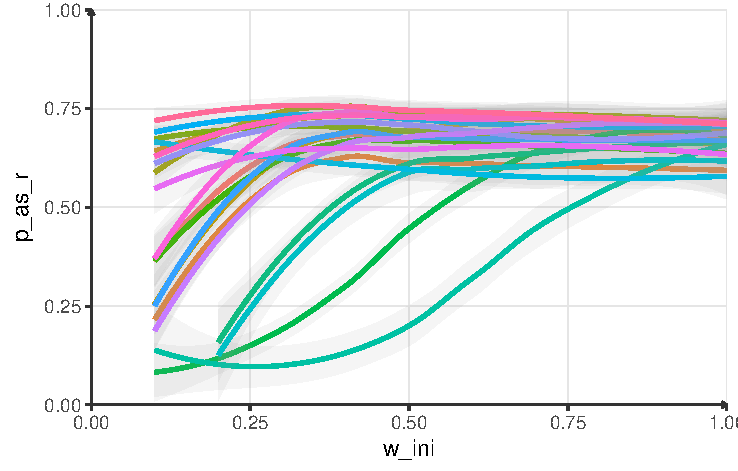
\includegraphics[width = \textwidth]{./2_PP/Figures/Individual/w_ini_p_as_r.pdf}
\caption{Effect of memory of water availability on proportion of active tissues in roots. \textit{Plastic-optimisation}. Each line correspond to a local regression fitted for all memory combinations for a given parameter set. Water availability memory is given in percentage of maximum exchange rate, absolute values may change between parameter sets.}
\end{figure}


\begin{figure}\label{fig:l_ini_p_as_r}
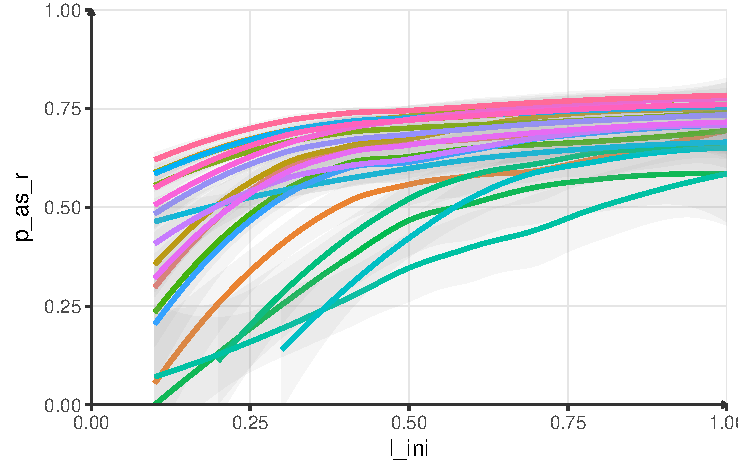
\includegraphics[width = \textwidth]{./2_PP/Figures/Individual/l_ini_p_as_r.pdf}
\caption{Effect of memory of water availability on proportion of active tissues in shoot. \textit{Plastic-optimisation}. Each line correspond to a local regression fitted for all memory combinations for a given parameter set. Light availability memory is given in percentage of maximum exchange rate, absolute values may change between parameter sets.}
\end{figure}

The combine effect of the two axis of plant resource availability memory is observed by plotting the phenotypes (on the 2D space of active tissue allocation) of four contrasting memories for all parameter sets (figure \ref{fig:memory_n_phenotype}). There is clear clustering of the four memory profiles, with some overlaps due to the fact that multiple parameter sets are plotted at the same time. The memory of low availability (\textcolor{myRed}{$\bullet$}) has a much larger distribution area than others, suggesting the relative instability of this profile within the "estimated net gain landscape". Memory of low availability for both resource drives plant toward very conservative strategies (need some values here) than other strategy. High expected availability of at least one resource increases allocation to active tissues to both organs. This confirms the positive effect of complementary resource (light for roots and water for shoot) of active tissue allocation in organs (see figure \ref{fig:l_ini_p_as_r}). Because of this, there is no highly unbalance phenotypes with high contrast between organ specific allocation emerging from the \textit{plastic-optimisation} allocation in \model. There is general coordination, but the balance between resource availability memories still impacts the position on the 2D, illustrated by the absence of overlap between low light - high water  (\textcolor{myBlue}{$\bullet$}) and high light - low water (\textcolor{myYellow}{$\bullet$}) phenotypes. In case of high resource availability and coordination, high investment in active tissues for both organ is achieved(\textcolor{myGreen}{$\bullet$}) and high light - high water), but the range of values is similar than for unbalanced memories(\textcolor{myBlue}{$\bullet$}) and high light - low water (\textcolor{myYellow}{$\bullet$}).

\begin{figure}\label{fig:memory_n_phenotype}
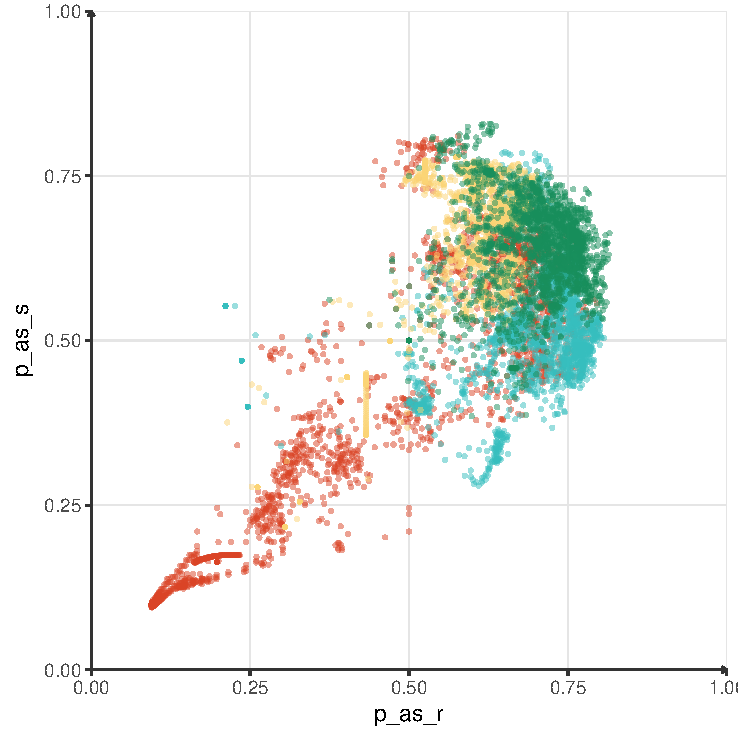
\includegraphics[width = \textwidth]{./2_PP/Figures/Individual/par_v_2D_points.pdf}
\caption{Impact of species memory on final phenotype in case of fully plastic allocation. \textit{Plastic-optimisation}. Each point corresponds to a plant phenotype for a memory syndrome for a given parameter set. Colours denote the memory syndromes.

\textcolor{myRed}{$\bullet$ low light - low water}, 

\textcolor{myYellow}{$\bullet$ HIGH light - low water},

\textcolor{myBlue}{$\bullet$ low light - HIGH water},

\textcolor{myGreen}{$\bullet$ HIGH light - HIGH water}.}
\end{figure}



\subsection{Discussion}

\paragraph{Allocation algorithms}

The pre-calculation of phenotypes, avoiding any phenotypic drift, allows for all allocation rules to grow plants with close performances. Nevertheless, the plastic algorithms show changes in RMF at the end of the simulation when the light:water balance starts to shift. This consistent shift in RMF for all three plastic allocation rules (with low variation of the other plastic dimensions) suggests the sensitivity and importance of this phenotypic axis. On the other hand, the other plastic dimensions benefit the plant growth suggesting that they also play a role in the tissue efficiency. While both the RMF and the proportion of active tissues can change the exchange area, only the proportion of active tissues can change the tissue efficiencies. Because the RMF shows similar levels of variation and range in both \textit{fixed} algorithms (RMF is the only plastic dimension) and \textit{plastic-optimisation} algorithm (see table \ref{table:variability-rmf}) the allocation of active tissue in the latter algorithm does not compensate for change in root:shoot allocation and is not used to increase the area of the limiting organ. This is confirmed by the fact that memory of low-light conditions (\textcolor{myBlue}{$\bullet$} in figure \ref{fig:memory_n_phenotype}) lead to lower allocation to active tissues than high light conditions (\textcolor{myYellow}{$\bullet$}). In the case of fully plastic plant trying to optimise their growth, the vegetative phenotypic dimensions do not fulfil the same functions: the RMF is used to adjust the balance between the resource exchanges while the change in active tissue proportions are related to the tissue and whole plant efficiency. This contrast in functions looks opposed to what is often observed in empirical studies wher eshoot:root ratio and SLA (here controled by the porportion of active tissues) respond in the same direction to increase the leaf area and compensate low indident light \parencite{ryser_consequences_2000, poorter_causes_2009, poorte2_biomass_2012}. This discrepency reveals a limitation within the plastic-allocation algorithm: the balance function is mostly supported by changes in root:shott ratio while the proportion of active tissues (controlling SLA and SRL) controls the tissues efficiency. The low proportion of active tissues in low resource (\textcolor{myRed}{$\bullet$} in figure \ref{fig:memory_n_phenotype}) indicates a selection of more conservative phenotypes when the resource is scarcer. This is in agreement with the Grime's triangle \parencite{grime_evidence_1977} and large scale empirical studies \parencite{wright_worldwide_2004}. In contrast with the conclusions of \cite{ryser_consequences_2000}, here the full phenotypic plasticity of the \textit{plastic-optimisation} algorithm is driven by similar constraints than the long term selection processes. This can be explained by the design of the trade-ofs that drive the gain function (see chapter \ref{part:model}). Therefore there are strong constraints on the tissue allocation, but low constrains on the root-shoot allocation. Additional constraint of this dimension can be added by considering other functions of each organs (such as nitrogen absorption by roots). In addition to this imbalance in constraints, the mean organ approach can also explain this behaviour. Approximating the properties of the canaopy by considering one mean organ leads to: a low impact of the plastic allocation on the SLA and SRL if the already existing compartments are large relative to the growth, a high importance of old tissues, while most of the exchange activity is generally produced by freshly grown tissues. Also, the rapid growth and turn-over in numerous parameter sets also authorises rapid plastic response on the RMF dimension (see also the rapid oscillations in the figure \ref{fig:comparison_RSR} top left panel)), diminushing the need for tissue specific adjustments. A stronger calibration of gross production and turn-over rates should reduce this effect. Finally the optimisation function may be too strong and plants may not always go for the optimum allocation but for the fastest and most competitive choice (see \cite{farrior_resource_2011,dybzinski_evolutionarily_2011, farrior_competitive_2014}). If this is not a problem in the context of this simulation where the memory is used to drive the default phenotype of the plant, it would be problematic in the context of plastic responses.
%
%Why ? trade-off too strong of tissues, but not enough of root:shoot ratio ? Why ? mean organ appraoch: effect on already produced tissues, lack reactivity and amplitude,
%+ rapid growth allowing rapid changes of RSR ratio
%+ lack of constraint on roots:shoot ratio
%+ optimisation may not be the best function (despite similar approaches: optimisation over time)

%The roles of PA and RMF ? balance versus efficiency. Because same variability of RMF.

%Different functions.


% YET TO BE EXPLORED
%rapid convergence.\\
%
%Cost and gains\\
%
%Diversity of phenotypes\\
%
%Crossed and symmetric influence: the respective efficiencies cannot be analysed independently.\\



\textbf{The different allocation algorithms impact the vegetative phenotype in different ways, but with similar performance when any phenotypic drift is avoided. But, the plasticity along the three main dimensions of the plant vegetative phenotype (PAR, PAS \& RMF) seems to have different objectives. While the RMF is the main adjustment variable to respond to changes in equilibrium, the proportion of active tissues is more closely related to the amount of resources and tissue efficiency.  However, it does not reproduce increases in organ area by changes in traits when the related resource is limiting. Multiple factors can explain this partial discrepancy with empirical results. The model still can be used to better understand the role of the memory as a driver for the phenotypic development, and the effects of the plasticity (particularly the RMF dimension) on plant performances.}

\paragraph{Strategies and coordination}

The \textit{plastic-optimisation} allocation algorithm allows for interesting insights on how the different resources affect the theoretical optimum phenotype. The increase in resource levels leads to an increase in the allocation of organic matter to the active tissues. While this is commonly demonstrated, the indirect effect of one resource on an organ that is not limiting for this resource is less often studied. A higher perceived resource availability drives plants to have a higher proportion of active tissues in both gathering (\textit{i.e.} leaves for an increase in light availability) and other organs (\textit{i.e.} roots for an increase in light availability). The indirect effect of an increased resource level on the non gathering organ can be explained by two mechanisms: a shift in the limiting organ or an increasing gross productivity. The former mechanism is related to the equilibrium maintenance by increasing the exchagne area of the newly limiting organ (or reducing the exchange area of the non limiting organ, see \cite{liu_biomass_2004} for an example, or \cite{grassein_plant_2010}). However this type of response is unlikely considering this implementation of phenotypic plasticity, as the changes in exchange area are mostly driven by the organ biomass rather than its proportion of active tissues (see previous paragraph). The later mechanism is more in line with the observations of the behaviour of \model (figures \ref{fig:memory_n_phenotype} \& \ref{fig:l_ini_p_as_r}). It explains the increase in active tissues in both organs by an increase in the exchange rate of the gathering organ, allowing a better productivity and a less conservative strategy for both organs. 

Such allocation pattern could explain coordination between organs, as the cost of the respiration and turn-over are compensated globally by the gross productivity, and allows divergence from the optimum of the isolated organ functioning (see chapter \ref{part:model} for details on the organ trade-offs). However this coordination along a fast-slow axis asks the question of the stability of this strategy. Indeed, the high investment in active tissues observed suggest that the turn-over and respiration costs are high, and a loss in efficiency based on an incorrect estimation of condition could have strong negative effects. 



%fast-slow

%coordination, not only the limiting organ that is impacted \cite{wahl_phenotypic_2001}

%grassein (similar response: lowerleaf density when water treatment 
%+ Liu

%... nothing here yet, the idea was to show that the "strategy" of the species conduce to slow and fast archetypes. Should be able to show that with some memory simulations.\\

%But not equal distribution along the axis probably.


\textbf{The allocation trade-off allows for strategies from the fast-slow spectrum to arise for the shoot and roots based from the perceived condition availabilities with some degrees of coordiantion, in a coherent framework. Such allocation mechanism can explain coordination thanks to shared cost and increase efficiency when the resource is available. The potential instability of the phenotypes may lead to discrepancies between the \textit{plastic-optimisation} algorithm and performance landscape. }

\paragraph{The memory concept}

The model \model brings a new approach to agent-based models and plasticity by integrating the resource availability estimation directly as a parameter for the plant development strategy. Despite requiring certain adjustment for an integration with full plasticity (in RMF and organ specific traits), it reproduce a certain pattern of coordination and overall resource use strategy along resource gradients. It also makes a bridge between the mechanistic approaches, that use species specific parameters measure on individual plants, and species distribution models (SDMs) that focus on abiotic conditions \sidenote{new SDMs now integrate biotic interactions as well as other ecological processes, as suggested by \cite{guisan_predicting_2005}.} and how species distribution match climatic variables. This new framework can allow more exploration at bigger scales with numerous species, that is often the limitations of such agent based models. However, to make this step, further work is needed on the general assumption that these estimation of conditions coupled with the gain function give good proxy to the plant development. There must be a strong positive correlation between the memory, the developed phenotype and the plant performance. 

While this verification seems obvious, difficulties can arise if you consider plant with different levels of plasticity. A non plastic plant will certainly require the same memory as a plastic plant that will be able to adjust this memory. The former should conciliate the memory (and therefore the phenotype) matching the conditions of it growing period with values that limit risks of negative growth outside this favourable period. A mean value of the experienced condition during the growing period is certainly a good value for the memory. This also rise the question of the ontogeny in these models that often consider fixed allocation parameters. In \model , ontogenetic shifts can be mimic under \textit{plastic-optimisation} by having default allocation parameters different from the ones computed by the optimisation algorithm \sidenote{limited here by a first simulation cycle, see methods for details.}. In the other hand, plastic plants better have a memory that matches the conditions at the early stages of growth, and let the plasticity drive the allocation for the continuation of the development. Also, while the structure of the model lets a door open for the integration of heritability mechanisms (hrough epigenetic modifications) that are expected to play an important role in the adaptation to the global change, those differences between plastic and non plastic plants may impact the integration of plasticity. This argument also encourage to find alternative solution to model plastic traits. Based on the review by \cite{crisp_reconsidering_2016}, the concept of memory can be conserved, but adapted to be more driven by stress and stress response/recovery than actual resource values. The knowledge of molecular mechanisms of the plant functioning must better inform the modelling routine that is too focused on mathematical andtheoretical approaches. The advantage of such specific memory mechanism is that it can be stress specific \sidenote{as suggested in the section \ref{part:model}.} and allows the integration of heritability.

\textbf{The concept of memory, even if it allows the contrasting phenotype in a continuous space, should take a different form to suit multiple plasticity strategies and integrate a form of heritability. The molecular mechanisms of plastic responses are better understood and provide solid foundations for new organ specific plasticity.}

\textbf{The model \model integrates trade-offs in resource use driven by the memory in resource availability. The investigation of the allocation patterns driven by the \textit{plastic-optimisation}   algorithm under the assumption of maximisation of the daily growth demonstrates different roles of the phenotypic axes: the RMF largely controls the equilibrium between shoot and root total activities, while the proportion of active tissues are related to the tissue efficiency as well as the overall plant efficiency and resource use strategy. While the fast-slow gradient along resource gradients is reproduced, and organ partial coordination explained, plastic responses to answer quick changes in resources are likely to not be reproduced due to a lack of constraints on the RMF dimension. THe effect of the different algorithm, plasticity strategy and resources affect the plant performance still have to be investigated. Despite the evidences that the \textit{plastic-optimisation} allocation mechanisms needs adjustments, the \textit{fixed-equilibrium} algorithm offer sa great tool to study the effect of plasticity on plant performances and best strategies.}


% ##################################################################################
\chapter{Individual performance, plasticity and variable conditions}\label{chapter:individual}

The previous section highlighted the ability of the model to model growth, but also the importance of species specific parameters. While the plasticity mechanism did not replicate to a full extend (stable and higher amplitude) the phenotypic changes between the different conditions, there were some changes both in traits and in growth, leading to a higher selection rate. Considering the importance of species specific parameters and their potential impact on growth, these differences between plastic and non plastic allocation rules should be investigated in an extended manner. The specific roles of strategy and memory on the multiple components of plant growth need to be disentangled to draw better hypotheses on the role of phenotypic plastic on plant performance and coexistence. The role of resource availability on these mechanisms also needs to be interrogated. The effect of plasticity on coexistence can also be approached with respect to relative performances and contraction of the strategy space.

This chapter tends to answer these questions with simulations of individual plants with diverse strategies and under multiple allocation rules. To simplify the approach and focus on the interaction between species strategies and allocation algorithm, the plasticity will be model as discrete mechanism (tau = 0 for all plastic allocation algorithms).

\section{Individual performance: between strategy, memory and plasticity}\label{section:landscape}

This first subsection focuses on the link between the phenotype and the plant performance. The plasticity and allocation mechanisms can affect both the link between phenotype and performance and the distribution of the existing phenotypes.



\subsection{Method}

\paragraph{Parameter sets}
Because little differences are found between accepted parameter sets for the three main algorithms, parameter sets selected for the \textit{non plastic} algorithm are used for all algorithm. To reduce the number of simulations but have a measure of the genericity of the observed patterns, 20 parameter sets are selected among the accepted parameter sets for the \textit{non plastic} allocation algorithm. As mentioned in the previous section, the parameter sets have been selected for only one species-specific and therefore an additional step was used to filter out the parameter sets that could lead to high biomass values. For each parameter set, simulations of diverse phenotypes run for 100 days of 15 hours with favourable temperature conditions (20 \celsius) along resource availability gradient. The parameter sets are selected based on the maximum biomass of all simulated plants. One parameter set is randomly selected for each of the 20 brackets between 0 and 2 grams of total biomass.

\paragraph{Strategy space sampling}
To better understand what make a plant perform in the model, a multitude of phenotype needed to be tested. Tested phenotypes are distributed regularly along the three axis of the strategy space (proportion of active tissues in root, proportion of active tissues in shoot, proportion of roots) between extreme values (respectively (0.1, 0.99), (0.1, 0.99) and (0.1, 0.9)) for a total of 3375 combinations ($15^{3}$).  Because the RSR is defined by the memory, and in this set of simulation experiments the RSR is defined before, the species memory needs to be computed afterwards. There is an infinite number of couple of memory values that can match a given RSR. Also, the projection of conditions is sensitive to both memory and experienced conditions, therefore the choice of memory can affect the relative sensitivity of species to changes in external conditions and alter the model behaviour. Because the role of memory is not the focus here, and because there is much more focus on the role of the plasticity as a mechanism (as opposed as a strategy with various values of \texttt{tau}), the parameter \texttt{tau} is set to 0. This ensures that only the starting phenotype and the experienced conditions play a role in plant performance.

\paragraph{Simulation set-up}

For each phenotype a pot simulation is ran for 100 days of 15 hours under 4 millimetres rainfall and 120 Watt per square metres and per hour with the 4 main allocation algorithms (\textit{non plastic}, \textit{fixed-equilibrium}, \textit{fixed-optimisation} and \textit{plastic-optimisation}. Two resource levels are tested for each simulations. The low resource availability conditions correspond to a reduction by a factor 4 of resource influx, but the day length was conserved.

\paragraph{Projections}

To visualise the performance landscape (plant performance relative to biggest plant as function of its phenotype) the performance of best phenotypes are projected against the 3 plans that compose the phenotypic space. Such projections are preferred to 3D alternatives as they work better with static visualisation and when most of the space is occupied. Alternative axis are defined to facilitate the interpretation and description of the performance landscape: the organ strategy plane(PAR-PAS plane) can be transformed into strategy balance (difference between PAS and PAR) and "speed" (in sense of Reich \parencite{reich_world-wide_2014})(mean allocation to active tissues).

To study the potential effect of resource availability and or allocation mechanism on the link between strategy and performance, an aggregated measure is designed: the \textemph{gravity center} of the phenotypic space is defined as the average phenotype weighted by the relative performance of each phenotype. It can be defined with respect to the initial strategy, or to take into account the plasticity, to the final position in the phenotypic space. Shift of this gravity center within the projection space inform of translation of the performance landscape.

\paragraph{Normalisation}

Biomass measures are relative to best performing non plastic plant (to remove the general parameter set effect on growth) and compare (within each condition) the effect of allocation algorithm. %Plasticity lead to an increase of average relative biomass, especially full plasticity. However, few values above 1, in fixed conditions there is real additional value of plasticity compare to fixed allocation.\\


\subsection{Results}

\paragraph{Performance landscape}
The effect of species specific parameter on growth are first studied with the analysis of the performance landscape drawn by the growth of plants uniformly distributed in the strategy space.

%The allocation phenotypic space is three-dimensional, but only two dimensions are represented (proportion of active tissues in roots (PAR) and proportion of active tissues in shoot (PAS)), while the best value of the third (root mass fraction) is used for the projection of the biomass.

\begin{figure}\label{fig:best_phenotypes}
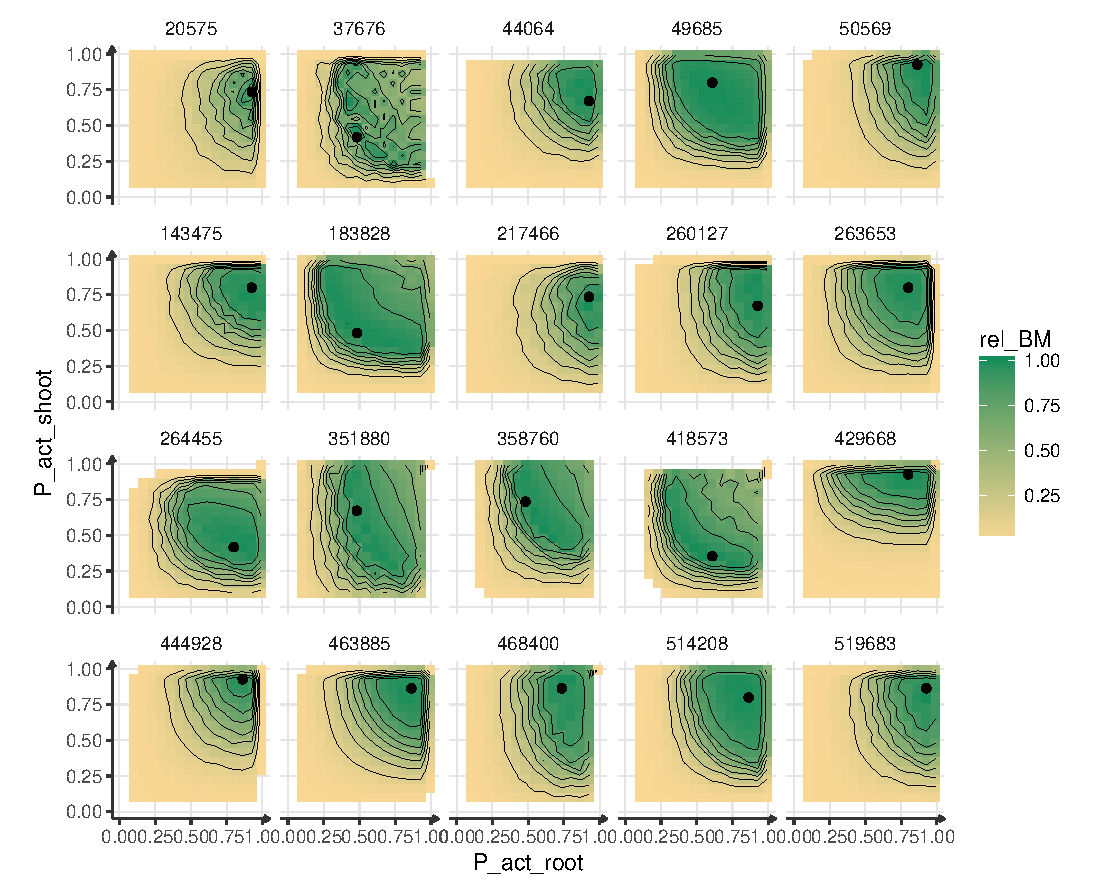
\includegraphics[width = \textwidth]{./2_PP/Figures/Landscape/landscape_PAR-PAS.pdf}
\caption{Projection of best phenotypes (varying RMF) on the 2D PAR-PAS plane for each parameter set. Points identify the optimums. \textit{Non plastic}.}
\end{figure}

 On the tissue allocation plan (proportion of active tissues in leaves and roots) (see figure \ref{fig:best_phenotypes}), the best performing phenotypes present a bean shape. This shape covers a good fraction of the space, in the center and sometimes top-right corner (high active tissue allocation) of the 2D space, while other corners are ignored. Too low values for any of the organs lead to a limited growth. For certain parameter sets, the top-right corner, corresponding to high resource acquisition strategies, has lower growth values than the center. They have lower growth values than phenotypes with similar values for one of the organ and lower value for the other organ.  %This shape suggest that relative importance of organ efficiency is lower than other criterion such as equilibrium and overall performance (see section \ref{chapter:modelling_PP} paragraph \ref{subsection:match} for the discussion on the components of plant performance). On this plane, the lowest values of plant biomass are characterised by low values of active tissue allocation. 
 

Projection of the best phenotypes over the three planes also gives information on the importance of the ignored variable on each plane. If the contrast between the growth projected phenotypes is high, at least on the main dimension is crucial for the growth. If the contrast is lower when the variable is ignored (\textit{i.e.} the best value is used) then the projected variable is likely to be important. The projection on PAR-RMF and PAS-RMF (see figure \ref{fig:projections}) planes show higher contrast between phenotypes relatively to PAR-PAS plane, therefore the RMF is a more sensitive variable than the allocation factors to active tissues in organs.


%Higher resource: contraction of the landscape, toward faster species. Moving optimum and moving gravity center. Transition to optimum shifting and difference between allocation rules.

\paragraph{Optimum shifting}

Introducing resource availability variations and plasticity can impact the shape of the performance landscape.

A shift of gravity centres can be observed between the two resource levels in all allocation algorithms (see figure \ref{fig:gravity_shift_resource}, the four panels). \textit{Non plastic} and \textit{fixed} algorithm show similar trends with an increase of proportion in active tissues in both organs. This change toward more exploitative tissues is consistent and is observable for all parameter sets but one. The \textit{plastic-optimisation} algorithm show drastically different responses of gravity center of phenotypes. There is little change in shoot proportion of active tissues, but a consistent reduction of active tissues in root system, and a reduction of root mass fraction (data not shown). These two responses indicates a net reduction of root activity in favour of shoot activity. Two things must be taken into consideration while looking at theese results: (1) the gravity center is computed from final position into the phenotypic space, not the starting position, (2) because \textit{plastic-optimisation} algorithm allows changes in traits that are represented (PAR and PAS), shifts along these axis can be driven by the plasticity mechanisms and not neceseraly only performance differences. Similar representation of the gravity center computed from the initial phenotype (not shown) shows similar response for the three first algorithms, and no apparent shift for the \textit{plastic-optimisation} plasticity.

\begin{figure}\label{fig:gravity_shift_resource}
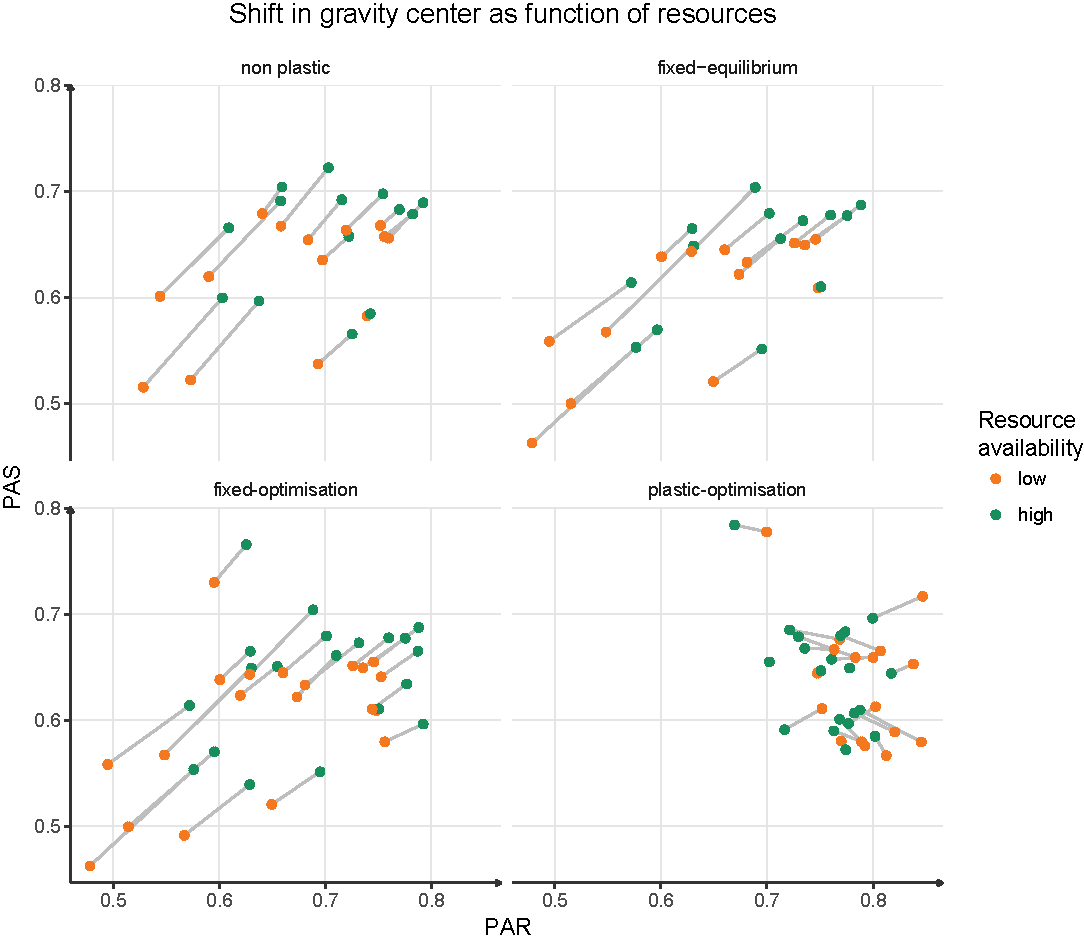
\includegraphics[width = \textwidth]{./2_PP/Figures/Landscape/ld_gravity_resourceall.pdf}
\caption{Shift on the 2D phenotypic space of the center of gravity as function of resource availability. The center of gravity is defined as the average phenotype weihted by the relative biomass, and characterises the performance landscape. \textit{Non plastic}.}
\end{figure}

\textit{Non plastic} and \textit{fixed} plasticities respond the same way to a shift in resource availability. However, we can note that the gravity centres have lower proportion of active tissues for \textit{fixed} allocation algorithm compared to the \textit{non plastic} one.

%
%Shift due to plasticity -- timing only ?
%+ shift (not fully significant in high resource availability) toward more exploit shoot and less exploit root. What does that mean ? higher tissue efficiency authorized by less limiting water ?
%
%Where is the optimum ?  what makes an optimum ? Why is it important ? -- beter understand how plasticity works and can improve plant performance.
%
%What are the sensitive dimensions ? and why ? 
%
%then moving optimum and why ?
%
%Moving optimum 2D: why ?
%
%What is the plastic-optimisation doing ? Wrong phenotype ? Wrong projection ? Wrong strategy or wrong RMF ? 

%\paragraph{Phenotypic space contraction}
\paragraph{Productivity changes}

Plastic allocation lead to an improvement in mean biomass of all individuals for all three plastic allocation algorithms (see figure \ref{fig:mean_BM_pl}). The \textit{fixed-equilibrium} plants are 2.5 times bigger in average than \textit{non plastic} plants (in low resource conditions, and up to 7 times bigger for \textit{plastic-optimisation} plant. These ratios are relatively similar for high resource availability. 

\begin{figure}\label{fig:mean_BM_pl}
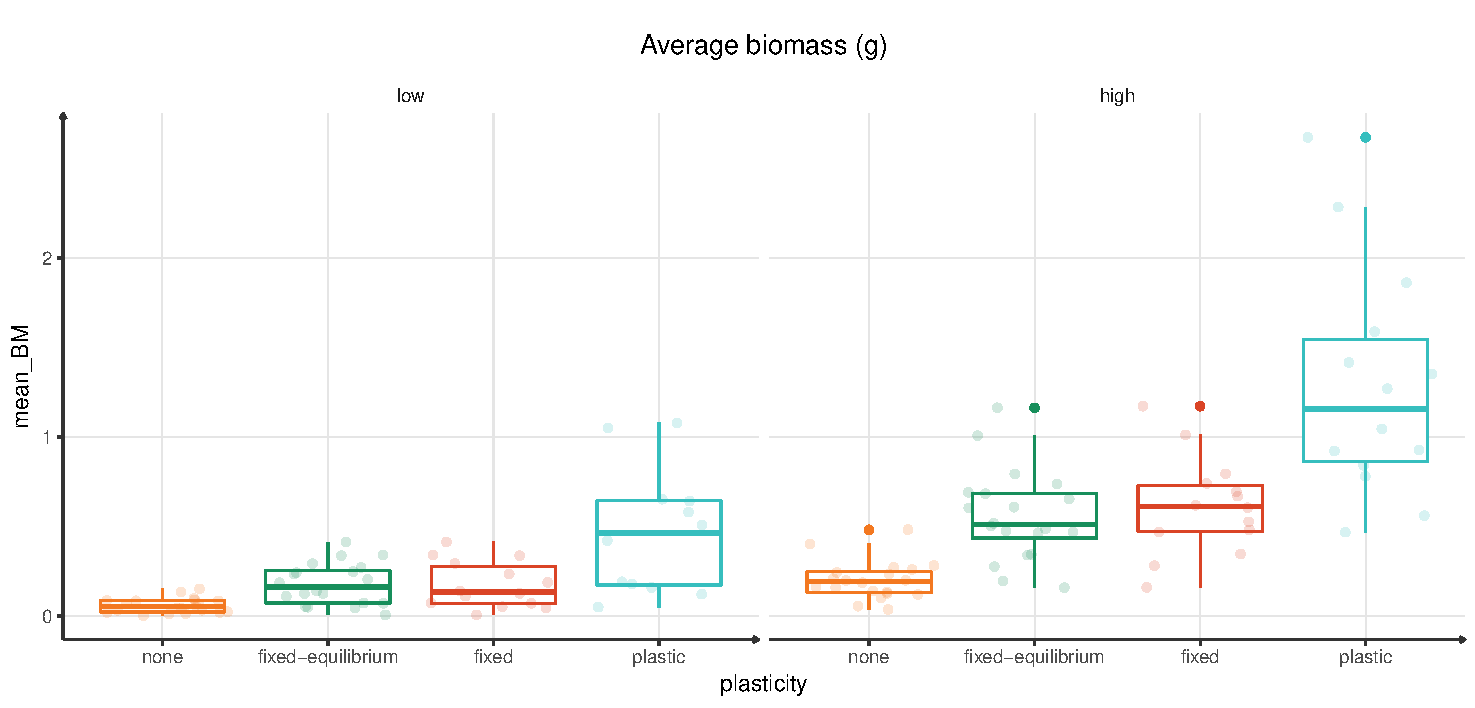
\includegraphics[width = \textwidth]{./2_PP/Figures/Landscape/plot_BM_allocation.pdf}
\caption{Mean relative biomass as a function of allocation algorithm and resource level.}
\end{figure}

However, the maximum biomass is only marginally improved with an increase of 6\% for \textit{fixed-equilibrium} and 8\% for \textit{fixed-optimisation} in low resource condition (see figure \ref{fig:max_BM_pl}). These percentages drop to less than 1\% in high resource availability conditions. The \textit{plastic-optimisation} algorithm even lead to a decrease in the maximum biomass averaging 10\% and 13\% respectively in low and high resource availability conditions.

\begin{figure}\label{fig:max_BM_pl}
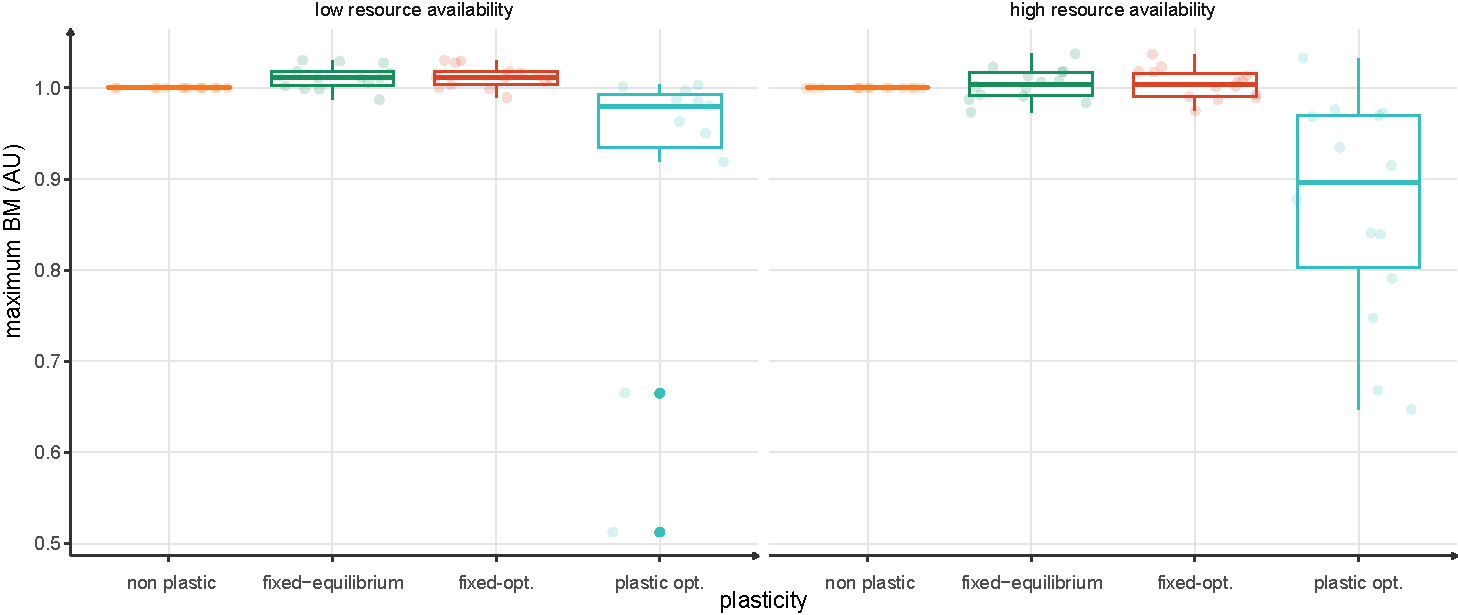
\includegraphics[width = \textwidth]{./2_PP/Figures/Landscape/plot_maxBM_allocation.pdf}
\caption{Maximum biomass relative to the \textit{non plastic} simulations, as a function of allocation algorithm and resource level.}
\end{figure}

\paragraph{Phenotypic convergence}

The effect of plasticity on the potential diversity is estimated by looking at the species that reach the range of 90\% to 100\% of the maximum biomass within the specific conditions (for each parameter set, algorithm and condition separately).

\begin{figure}\label{fig:species_richness}
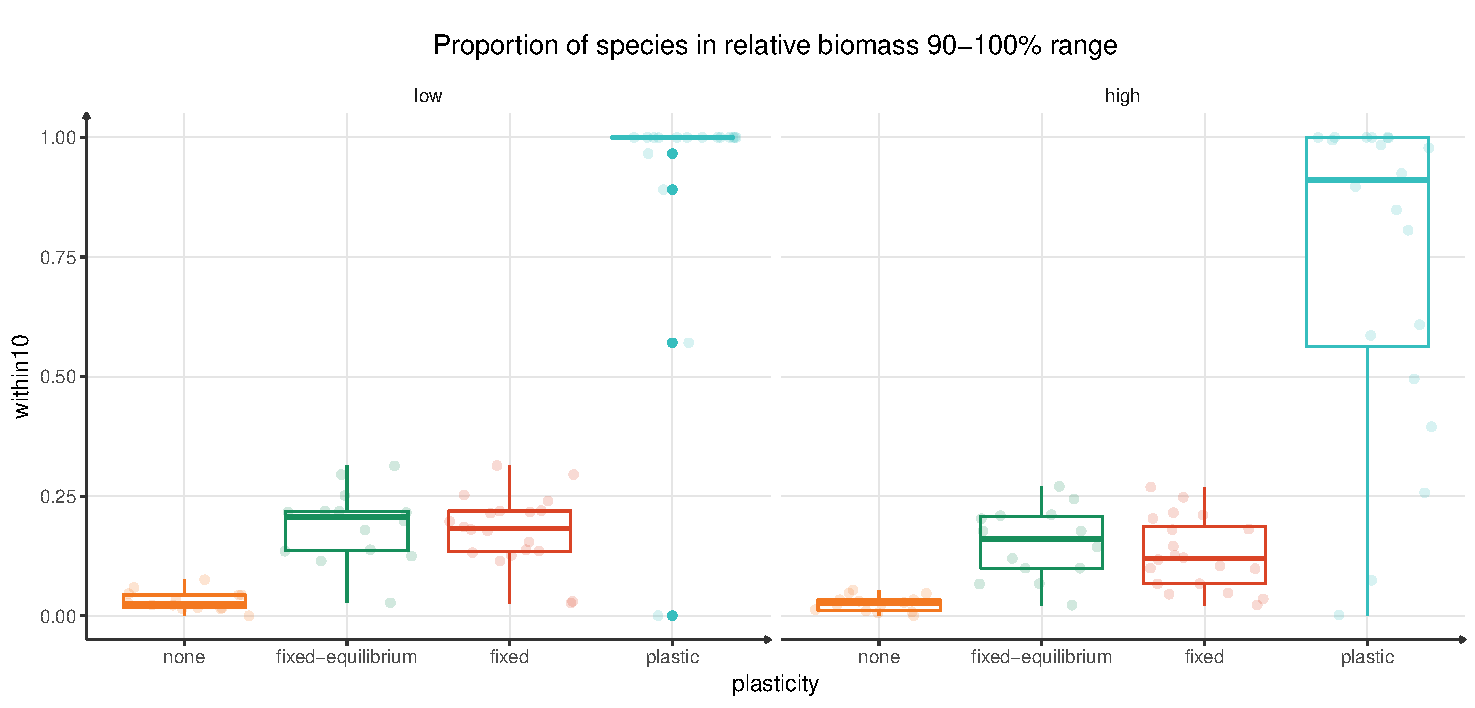
\includegraphics[width = \textwidth]{./2_PP/Figures/Landscape/plot_eveness.pdf}
\caption{Number of species within the range of 90\% to 100\% of the maximum biomass, as a function of allocation algorithm and resource level.}
\end{figure}

The number of species within this range is extremely low in \textit{non plastic} allocation algorithm simulations, with 1.4\% and 2.1\% respectively for low and high resource conditions. This percentage is greatly improved by plastic allocation algorithm and reach in average 9\% to 15\% of species in \textit{fixed-equilibrium} and \textit{fixed-optimisation} algorithm, while in can reach up to 100 \% for \textit{plastic-optimisation} algorithm, with a mean proportion of species with a top performance around 72\% in low availability condition, and up to 82\% in high resource availability condition.

\begin{figure}\label{fig:function_div}
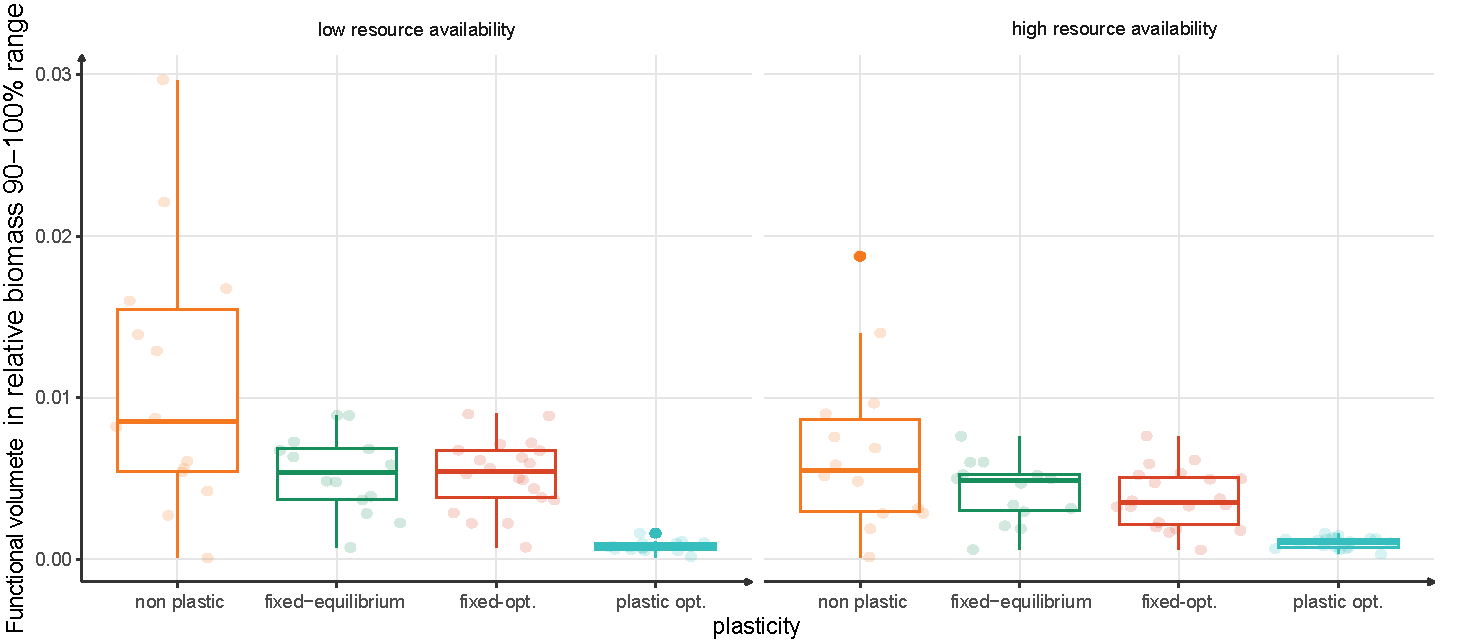
\includegraphics[width = \textwidth]{./2_PP/Figures/Landscape/plot_fdiv.pdf}
\caption{Functional volume occupied by the species within the range of 90\% to 100\% of the maximum biomass, as a function of allocation algorithm and resource level.}
\end{figure}

The functional diversity, estimated with the approximate volume of the top phenotypes, follows a opposite trend, with the highest value for the \textit{non plastic} allocation algorithm. \textit{Fixed} algorithms present half the functional volume of the \textit{non plastic} algorithm, and hte \textit{plastic-optimisation} algorithm has extremely low values five times lower than the \textit{non plastic} ones.



\subsection{Discussion}

\paragraph{Components of performance}

The study of the performance landscape puts in light the different components of \textemph{plant performance}. To understand how plasticity can play a role, it is important to understand what make a phenotype a good phenotype. 
% the main axis: 
On one hand, the extend of strategies (plan PAR-PAS in figure \ref{fig:best_phenotypes}) with high relative growth (green area) is high when the best  RMF is considered, while this is greatly reduced on plans that integrates RMF variability (see figure \ref{fig:perf_decomposition}). This result suggest the high importance on this axis for the plants performance. This can be explained by a stronger effect of this dimension on the exchange area through changes in organ masses, instead of organ densities (affected by PAR and PAS). The RMF fraction impacts the plant performance in two ways: by changing the \textemph{equilibrium} between shoot and root exchange activities, and by changing the global carbon loss rate (respiration and tissue turn-over) if the organ differ on this aspect. These two components may have opposed directions, as the limiting organ may also be the least efficient, and therefore the RMF could be greatly constrained if the two aspects have similar importance. The effect on the equilibrium is likely be more important as a wide range of RMF values can be observed for numerous datasets (data not shown), and plant with uncoordinated (low-PAS \& high-PAR, or high-PAS \& low-PAR, \see figure \ref{fig:perf_decomposition}) organs still present high biomass values, suggesting that the respiration and turn-over loss are less important than a balanced resource acquisition. 

%NEED THE DECOMPOSITION OF PLANT PERFORMANCE HERE

\begin{figure}%[tb]
    \classiccaptionstyle
\sidebysidecaption{0.60\textwidth}{0.3\textwidth}{%
    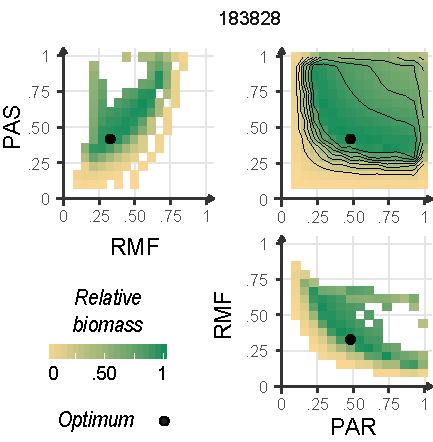
\includegraphics[width=1\linewidth]{./2_PP/Figures/Landscape/ld_space_ex.pdf}%
}{
  \caption[Projection of performance on phenotypic plans]{Projection for the parameter set 183828 of best phenotypes (according to the variable that is ignored) on 2D plans of the phenotypic space. The dots represent the optimum phenotype. White space indicates the absence of phenotypes able to survive until the end of the simulation (100 days). RMF: root mass fraction, PAR: proportion of active tissues in roots, PAS: proportion of active tissues in shoot. }
  \label{fig:perf_decomposition}
  }
\end{figure}

On the other hand the organ specific strategies are also important as low values for any of the organs (leaves or roots) lead to very low growth. Extreme high values can also be limiting, suggesting the existence of an optimum of the proportion of active tissue for the tissue efficient. This \textemph{optimum tissue efficiency} results from trade-off between active and structural tissues, driven by the relative importance of carbon gain (increased exchange area with active tissues) and carbon loss (increased respiration and turn-over with proportion of active tissues) that depends on models parameters and resource availability (that change the exchange rate).

\begin{marginfigure}\label{fig:function_div}
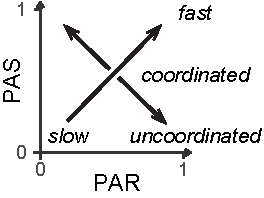
\includegraphics[width = \textwidth]{./2_PP/Figures/Landscape/ld_axis.pdf}
\caption{Alternative axes to describe the plant phenotypes on the plan PAR-PAR (PAR: proportion of active tissues in roots, PAS: proportion of active tissues in shoot). The slow-fast axis refers to the proportion of active tissues (close to the fast-slow strategies of \cite{reich_world-wide_2014}), while the orthogonal axis show how coordinated the plant is (see \cite{freschet_integrated_2015} for similar concept).}
\end{marginfigure}

However, meeting these tissues specific optima might not be sufficient, as the bean shape of the best phenotypes suggests, another component is relevant. Low values of proportion of active tissue in one organ can be compensated by a high allocation of active tissues in the other organ that allows a higher allocation in the low exchange rate organ. This confirms the importance of the equilibrium over the tissue specific strategies. But the shape also reveals a last component of the plant performances. The fact that species with high values of proportion of active tissues in both organs have lower biomass, is certainly due to a limitation of both resources (equilibrium is assumed), reducing the overall efficiency. 

From this visualisation of plant biomass as a function of the phenotypes, three main components play a role. The \textemph{equilibrium}, mostly driven by the changes in RMF is essential to the plant growth. This is explained by a reduction of the exchange rate of the non limiting organ that greatly reduces its organ specific efficiency (see figure \ref{fig:efficiency}). This \textemph{organ tissue efficiency}, driven by its effective exchange rate, respiration and turn-over, is also an important component of plant performance. Low values of allocation of active tissues greatly reduces this efficiency, but it can be compensated by bigger organs. However, such mechanisms can affect the overall efficiency defined as the average mean of organ realised efficiencies (taking into account resource limitations) weighted by the organ masses. Finally, the \textemph{speed} of the plant, or the overall resource acquisition rate, admits an optimum that is between an over-capacity leading to a co-limitation of resource on both organ reducing their individual efficiencies, and the under-capacity, leading to a sub-optimum use of resources and letting space for competition.

%NEED FIGURE OF EFFICIENCY: 

% the coordination

% the speed

%If equilibrium is a driving mechanisms in plant performance, for any given strategy (PAR-PAS plan projection) the best phenotypes has a RMF values that guarantee the functional equilibrium. However, for each strategy there is a notable difference between the RMF of best phenotypes  and the RMF of phenotypes the closest to the equilibrium. This disparity is positively related to the strategy balance: best phenotypes with higher active allocation in shoot than root have lower allocation to roots than required for functional equilibrium. 


%%\textemph{equilibrium}, overall \textemph{speed} and overall \textemph{efficiency}.\\
%The main thing with equilibrium is the total resource use.
%
%Better too fast than not fast enough.
%
%Explain the memory stuff in previous section: low-low compared to low-high, the second one lead to overall higher productivity (lack of one resource compensated by higher allocation to the related organ) that can support more active tissues. 
%
%The role of RMF: controlling variable, more sensitive than PAR and PAR but because bigger impact on balance: wide range on RMF values with similar performance: RMF value in itself is not that important: equilibrium is.
%
%Shifts in optimum, is it because plasticity provide more efficient functioning supporting more exploitative strategies, or side result from convergence that do not contain the previous optimum ?
%
%Convergence, relative species diversity and functional diversity.

\paragraph{Convergence to subspace}

The phenotypic plasticity allows species to move within this performance landscape along certain axis. It is is often perceived with a species-centric perspective, that is to say, that plasticity is seen as variations in the species mean phenotype. However, in the context of community ecology, it is also interesting to try to see how it not only affect individual species but shape the community distribution in the strategy space. The plasticity relies on changes of default phenotypes toward "better" strategies in the context of the given conditions, therefore it implies that if it exists an optimum subspace (one strategy or an ensemble of strategies) species will converge toward this subspace, distorting the functional space. Environmental variations and plant interactions aside, in a constant environment the \textemph{performance landscape} is fixed. As a consequence, the plasticity benefits to the plant in a static manner, that is to say, it is only a tool to reach a better phenotype where the plant stays in if conditions do not change. This can be related to spatial heterogeneity that would lead individuals from the same species to adopt different phenotype to acclimate to the particular conditions of their spatial situation. It is opposed to the perception of a more dynamic phenotypic plasticity as a tool for a given individual to cope with temporal variations in environmental conditions. These two aspects are further discussed in the following section, while the effects of the contraction of the phenotypic space are discussed now.

\begin{figure}\label{fig:convergence}
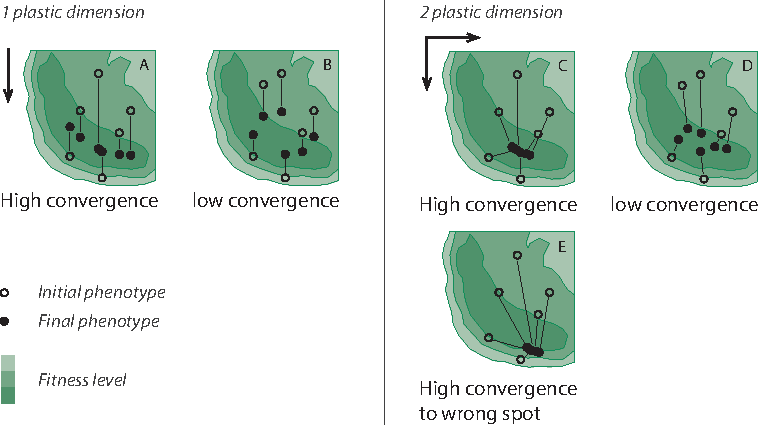
\includegraphics[width = \textwidth]{./2_PP/Figures/Landscape/ld_convergence.pdf}
\caption[Convergence patterns]{Convergence patterns on a 2D phenotypic fitness landscape, with 1 plastic dimension (A \& B) or 2 plastic dimensions (C, D \& E). Plasticity can lead to high convergence (A, C and E) with potentially high fitness evenness, especially in space with numerous plastic dimensions (A \& E), this is problematic especially if the point of convergence is not the optimum (E). Limits to high convergence are necessary to allow realistic functional diversity with plasticity (B \& D).}
\end{figure}

As just mentioned, the plasticity can be seen at the scale of the species assembly \sidenote{here I draw a distinction between species assembly that refers to all present species, and community that refers to the interacting individuals of the present species. However, some interpretations can be translated to communities.} as a contraction of the phenotypic space of the species assembly. This contraction has two main effects: the reduction of potential functional diversity and a reduction of growth rate differences. There is here an emerging trade-off between the \textemph{species diversity}, supported by lower fitness differences, and \textemph{functional diversity}, reduced by the contraction of the phenotypic space. However, if the plasticity reduces greatly the potential functional diversity (volume of the whole phenotypic space without considering filtering based on relative fitness), the realised diversity (expressed as the functional diversity of the species within the 90\%-100\% maximum biomass range) is less impacted because a large parts of the phenotypic space have low growth rate in the given conditions. Nevertheless, there is a reduction of the diversity of expressed phenotypes. Indeed, in this scenario of "extreme" plasticity ($\tau = 0$) the convergence is important on plastic dimensions while partial convergence would be enough to have good fitness (see conceptual figure \ref{fig:convergence}). Lower convergence on plastic dimension should lead to less compact phenotypic subspace while keeping relative fitness evenness. In the case of \textit{fixed-equilibrium} and \textit{fixed-optimisation} allocation mechanisms, this reduction of diversity is lower because only one axis is plastic.

Reduction of the phenotypic convergence can be achieved by other allocation mechanisms, differences in projection (different $\tau$ values leading to different projections) and plasticity costs. In heterogeneous system, this convergence is expected to be lower as heterogeneity will lead to different projections.

%Cost and distance, sensitivity to environmental cues as solutions to this problem. 
\paragraph{Limited dynamic gain}

The convergence of the phenotypes to a sub-space of lower performance lead to an increase in the mean biomass (see figure \ref{fig:max_BM_pl}). However, the maximum biomass is only marginally improved in \textit{fixed} plastic allocation simulations, and reduced in \textit{plastic optimisation} allocation simulations. This two contrasted results, show different effects of plasticity. The light increase can be due to either a dynamic gain or a static gain. The \textemph{dynamic gain} can emerge because the plant growth affects the resource availability, changing the optimum phenotype, and allowing plastic plants to follow this chaanges during time. It could also result from a \textemph{static gain} because the phenotypic plasticity allow a better resolution in tested phenotypes (the plastic axis are continuous while the phenoytpic space sampling was discrete). The role of plasticity and dynamic gain is explored in the following sections with temporal resource heterogeneity.

The reduction of the maximum biomass highlight the difficulty to find the optimum phenotype. Because, the growth mechanisms are reproduced in an exact manner in the plasticity algorithm, this mismatch is certainly due to a difficulty to project the future of resource availability. Because of that, it is possible that the gain in maximum biomass, mentioned above, due to static or dynamic gain is greater than it appears. The particular case of mis-projection in \textit{plastic-optimisation} simulations is discussed in the following paragraph. 

%Because of high convergence of \textit{plastic-optimisation}, no improvment of maximum biomass, but the \textit{fixed} alternative thanks to convergence limited to one phenotypic dimension (RMF) higher biomass: either higher resolution, or improvement due to \textemph{dynamic plasticity}. The role of dynamic plasticity benefit is explore in temporal variation simulations in the following section.


%Somehow I need to talk about the cost of being wrong. Can be observe in the delta heatmap on delta strat and delta w-ini: in this case there is less impact of being wrong of memory if you're good with strategy, because your not in different conditions...\\

%Potential effect on diversity: lower functional diversity, increase evenness. Leave highest fitness spot free. Why ? environmental cues or gain function ? Delta between projections ? \\

%Anyway, being good is stable conditions may useless if cannot survive or keep gain in other conditions. >> look along gradient if best species keep their rank.\\


\paragraph{Plastic exhaustion}

\textit{Plastic-optimisation} algorithm is characterised by a high convergence of the species within the phenotypic space, high mean biomass but maximum biomass lower than best \textit{non plastic} phenotype, and high potential species diversity. The convergence is expected and explained by the fact that all three traits are plastic and all species (for a given resource level) experience similar conditions leading to the computation of the same optimum. The absence of plasticity cost limiting the convergence leads to a phenotype concentration toward this optimum. This convergence explains both the high potential species diversity, as all species have very similar growth rate, and the relatively high mean biomass because only few species did not survive or had very little growth rate.

The fact that this plasticity does not translates into higher maximum biomass is surprising, especially considering the fact that RMF plasticity improves maximum biomass (see figure \ref{fig:mean_BM_pl}). Lag in adaptation is often identified as a limit of plasticity \parencite{dewitt_costs_1998, van_kleunen_constraints_2005}, nevertheless, in a constant resource influx experiment, and considering the high phenotypic flexibility of plants in \model, this explanation is unlikely. Another problem highlighted with plasticity is its adaptiveness. Evolutionary speaking, it is hard to imagine the emergence and maintenance of a plasticity mechanism (in a given context) if it is no adaptive. Yet, such process could be maladaptive in a new context. Because plasticity is not emerging, but imposed by the simulation set up, its adaptiveness can be interrogated. Here adaptiveness do not refer to a reduction of fitness due to plasticity, but to the capacity of the plastic mechanism to define an optimum (or at least better) phenotype. Plasticity as implemented in model has no explicit bias and all mechanisms involved in plant growth are simulated by the allocation algorithm. The sampling of phenotypes is random and could be source of uncertainty, but it is uniform and no consistent drift is likely to emerge from the noise introduced by such sampling. The last aspect of plasticity that can affect the adaptiveness of plasticity is the estimation of conditions. The estimation of conditions is based on resource levels experienced by the plant and by definition are exact, therefore the problem lies in the projection of these conditions and how they translate into resource uptake.


\begin{figure}\label{fig:exchange_volume_projection}
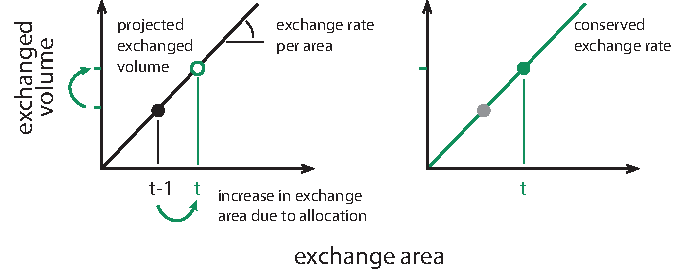
\includegraphics[width = \textwidth]{./2_PP/Figures/Concepts/exchange_volume_projection.pdf}
\caption{Projection of the water volume exchange after increase in exchange area at equilibrium and with no limitation.}
\end{figure}

In \model the resource availability is coded as an uptake rate per day and per unit of exchange area, and is computed as the resource uptake divided by the exchange area. This resource availability is supposed constant, and plants make the assumption that increasing their exchange area leads to a proportional increase in resource volume exchanged (see figure \ref{fig:exchange_volume_projection}).

\begin{figure}\label{fig:exhaustion}
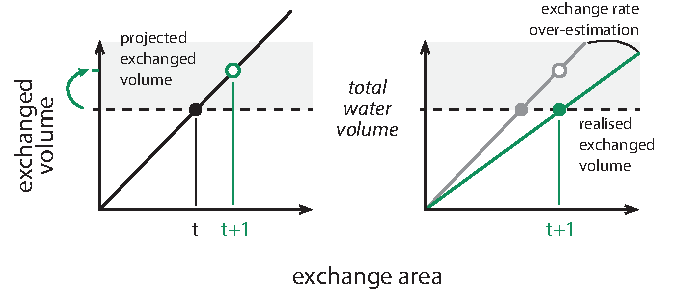
\includegraphics[width = \textwidth]{./2_PP/Figures/Concepts/exhaustion2.pdf}
\caption{Projection of the water volume exchange after increase in exchange area when total available water volume is limiting. The water volume exchanged cannot exceed the total available water volume, leading to a systematic over-estimation of water availability and offset between shoot and root activity.}
\end{figure}

However, in the case where a plant already absorbs all the available resource, then this assumption is not respected, and the uptake rate per area is lower than expected (see figure \ref{fig:exhaustion} right panel, realised exchanged volume does not match the projection because it cannot exceed the total volume of available water). This gap between perception and actual resource availability occurs because the plant is not able to perceive that the limitation cannot be compensated by a higher investment in the limiting organ. This behaviour explain a very high investment toward root and root active tissues in low resource conditions under \textit{plastic-optimisation} allocation (figure \ref{fig:gravity_shift_resource}). This gap\sidenote{this is different from a lag because it is not the result of slow changes in phenotype but comes from a default in the estimation of optimum phenotype.} is the cause of the \textemph{plastic exhaustion} phenomenon. Indeed, this constant over-estimation leads to constant discrepancy between the estimated optimum phenotype and the actual phenotype, and a larger allocation to root active tissues. This effect is particularly noticeable in the context of pot simulations where the water pool is limited. The absence of plasticity costs also favours such extreme behaviour. 

Despite this particular seemingly non-adaptive behaviour, the \textit{plastic-optimisation} algorithm is still interesting to study in community simulations. First, the presence of plasticity cost should limit such extreme behaviours. Second, in a context of competition in a larger environment, this aggressive search behaviour is likely to be an advantage against individual with less aggressive, or stable strategy. Finally, this mechanism emerges in constant influx conditions that allow growth, but its emergence should be reduced in variable environment where water shortage leads to reduced growth.

The plastic exhaustion mechanism seems to be contradictory with the previous observation that the proportion of active tissues does not increase when the related resource is limiting (see figure \ref{fig:memory_n_phenotype}), but it can be argued that it such extreme case, if the RMF has extreme values and is constrained by differences in tissue efficiencies. This is not verified however.

\textit{Plastic-optimisation} simulations expose this phenomenon with large effects, but it is probably present for simulations with other plastic allocations but with smaller effects. The difference in magnitude can be explained by a less effective growth in early stages of development for \textit{fixed} plasticities (when \textit{plastic-optimisation} is more efficient than fixed plasticities) that delay the time when the total volume is reached (time \textit{t} in figure \ref{fig:exhaustion}), and in average lower active tissue allocation in roots that leads to lower loss due to non-equilibrium.

\textbf{Plastic exhaustion is a specific limit of phenotypic plasticity as implemented in \model that relies on the assumption of constant exchange rate per exchange area. It has a large effect in the specific case of pot simulations. However, this phenomenon can be mitigated by plasticity cost linked to changes in traits, and can have adaptive value in a context of competition. Therefore, I argue that \textit{plastic-optimisation} algorithm  has low information value in the context of pot simulations with constant resource influx, but should still be studied in the context of community dynamics.}

%
%\paragraph{On diversity}
%Effects on diversity.\\ I would put that aside for now
%
%The potential functional diversity is amplified by the fact that many phenotypes that are not viable in any condition but becomes viable thanks to static gain of plasticity. These species exist in the context of the simulation because there is no cost to plasticity. Because species are uniformly sampled in the 3D, a lot of them could not grow in a lot of conditions ?

\paragraph{Resource availability}

results from this part\\
As expected the resource availability and the resource balance are key components of the plant growth, to which the plant phenotype needs to match. Aside from the increase in biomass, an increase in "speed" of optimum phenotypes can result from higher resource availability. This observation is in agreement with empirical data that demonstrate higher SLA and faster physiology in favourable conditions. This aspect was less obvious in the response of species under \textit{plastic-optimisation} allocation that shifted more in term of balance and RMF. This may be due to a change in the relative balance between both resources as their availability (from the plant perspective) are linked to the global resource levels by non linear relationships.

The fact that plastic plants (for \textit{fixed} allocation algorithms) show shifts of optimum strategies toward more exploitative phenotypes, in addition to the \textit{non plastic} optimum shifts, in conditions of higher productivity demonstrate the importance of these strategies for plant growth. However, the extend of this effect of conditions on optimum phenotype is susceptible to vary along a gradient. Indeed, because of the non linearity of relationships between resource levels and exchanges rates, and between exchange rates and growth rates, the link between the optimum phenotype and a resource gradient is likely to be non linear itself. In addition, phenotypic plasticity might also change the sensitivity of the phenotype to the resource level.

%Why we need to go for a gradient.

%\subsection{Extended discussion}
% level discussion}
%? about what ? Community dynamics ? pp impact of these dynamics ? coexistence of species


\paragraph{On functional diversity}

Can functional diversity be measured for plastic tratis: different effects on plastic and non plastic traits ?


%\paragraph{Nuances around plasticity}
%This analysis was conduced with drastic parameters of plasticity with plastic plants relying only on their perception of external conditions to develop their phenotype. The different results ... different directions and impact on potential diversity.
%
%Also, some species may not benefit from plasticity, especially if it has a cost, while others can benefit a lot from plasticity.
%
%The contrasting responses of the different algorithms highlight the importance of the allocation mechanism. However, the unique framework implemented in \model creates a variety of nuanced responses that are not all explored here. But, the continuous gradient of strategy between species relying on species memory only and species following their perception of external condition should be kept in mind during the interpretation of these results and following.
%
%\textbf{Subsection conclusion: bla bla bla}


% ##################################################################################
% ##################################################################################
% ##################################################################################


\section{Plasticity and variability of conditions}
%Question I try to answer: (use of schematics ?)
The heterogeneity of conditions is an essential mechanism for plant coexistence. Plasticity is likely to alter the effect of this heterogeneity on plant coexistence and relative performance. The impact of plasticity on this relationship between spatial and temporal \textemph{heterogeneity} of resources (here limited to water) and strategy dominance is explored with the model \model.\\

The phenotypic plasticity can impact the optimum strategy, but how does this effect impact the optimum phenotype along a resource availability gradient?
%Effect on optimum strategy: from previous conclusions and hypothesis to simulation method.\\

Is the contraction effect on species richness, functional diversity and productivity changing along such gradient?
%Then on diversity: how good strategies perform when it is plastic. Pool of species that exist in different conditions to get rid of the static effect.

\subsection{Method}

Because the coordination is shown to be less important than the equilibrium, the below-ground resource acquisition is expected to be important in mountain grassland under climate change scenarios, and extensive simulation plan come with high computational cost, only root strategies sampled in this part.

\paragraph{Simulation set-up}
For each of the 20 selected parameter sets, growth of 400 plants (20 PAR values between 0.25 and 0.95, and 20 memory values between 0.1 and 1) is simulated for 100 days in square pots of 12 centimetres deep and 90 centimetres wide (to avoid quick self-competition) in a temperature of 20 degrees celsius during the day of 15 hours, and 10 degrees during the night. The radiance is set to the high values of 122 Watt per hour and per square metre. Because \textit{fixed} algorithms showed similar results, and the \textit{plastic-optimisation} algorithm show strange results, only two allocation algorithms are simulated: \textit{non plastic} and \textit{fixed-equilibrium}.

\paragraph{Spatial heterogeneity}
Spatial heterogeneity of water level is mimicked by a gradient of water influx. The growth of all 400 species described above are simulated for \textit{non plastic} and \textit{fixed-equilibrium} algorithm independently in separated simulations where the water influx is regularly sampled between 0.05 and 7 mm per day (20 values).

\paragraph{Temporal heterogeneity}
Similar set-up is used for temporal heterogeneity simulations. Because the range of water influx used in the previosus simulation is too wide, a lower value is chosen as the mean water influx. This value of 1.3mm per day corresponds to a point around which there is variations in the optimum strategies for most parameter sets. It is also relatively close to average rainfalls in the Alps during summer. 

\subsection{Results: gradient of homogeneous precipitation conditions}

\paragraph{Optimum strategy}

To study the effect of plasticity on community identity along a precipitation gradient, we can look at the position of the optimum strategy (PAR) along such gradient with different allocation algorithms.

%%Only look at the median of best strat. Gravity center lower for fixed-equilibrium, because of a few more species living.

The effect of allocation algorithm is observed on all species by plotting the position of the median \textit{optimum} along the watering gradient that translates what part of the strategy spectrum (from conservative to exploitative) benefit from the simulation conditions. At the low end of the gradient, conservative species exhibit higher growth than exploitative species with a median optimum around 25\% of active tissues in roots for both the \textit{non plastic}and the \textit{fixed-equilibrium} plastic allocation. In the other end of the spectrum, for watering values above 1 mm per day, the \textit{optimum} reaches a high point (median around 90\% of active tissues for both algorithms) demonstrating better performance of the exploitative species in high resource availability conditions.  There is not apparent differences between algorithms and the optimum is conserved along the gradient. There is a similar shift with an increase of optimum water availability memory for \textit{non plastic} algorithm.


\begin{figure}\label{fig:gradient_strat_trend}
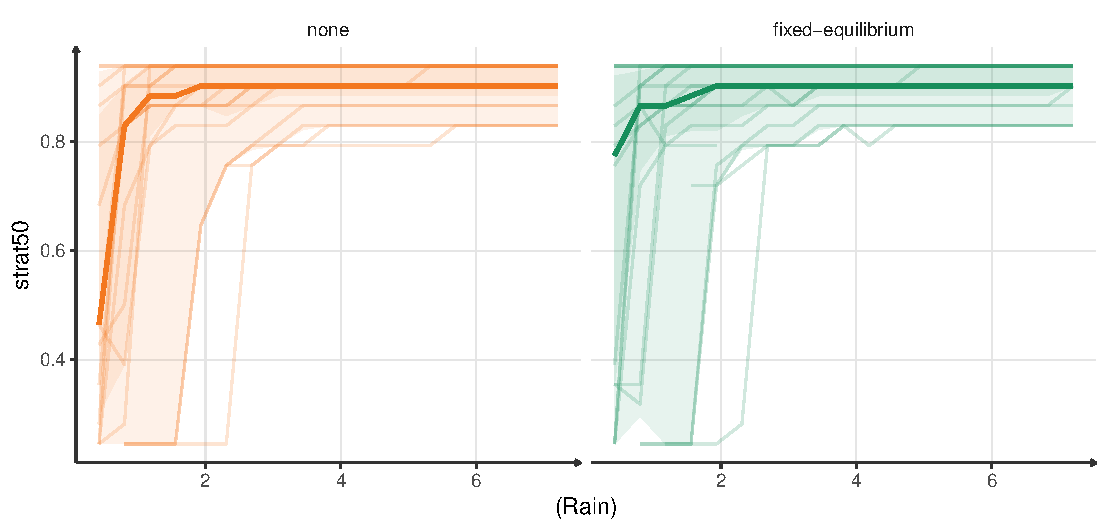
\includegraphics[width = \textwidth]{./2_PP/Figures/Rain/gradient_strat_trend.pdf}
\caption{Median (dark line \textbf{-}) optimum root strategy along the water treatment gradient for \textcolor{myOrange}{- \textit{non plastic}} \&  \textcolor{myGreen}{- \textit{fixed-equilibrium}} allocation algorithms. The light lines (-) correspond to the 20 independent parameter sets. The color ribbon marks the band between the 5th and 95th percentiles.} % Maybe I should change that so it is the 25th and 75th like for variable inputs.
\end{figure}

The memory of water availability of best performing phenotypes increases along the gradient under \textit{non plastic} allocation (see figure \ref{fig:gradient_w_ini_trend}, left panel), but the plasticity negates the effect of this species specific parameter and no lcear pattern can be observed (right panel).


\begin{figure}\label{fig:gradient_w_ini_trend}
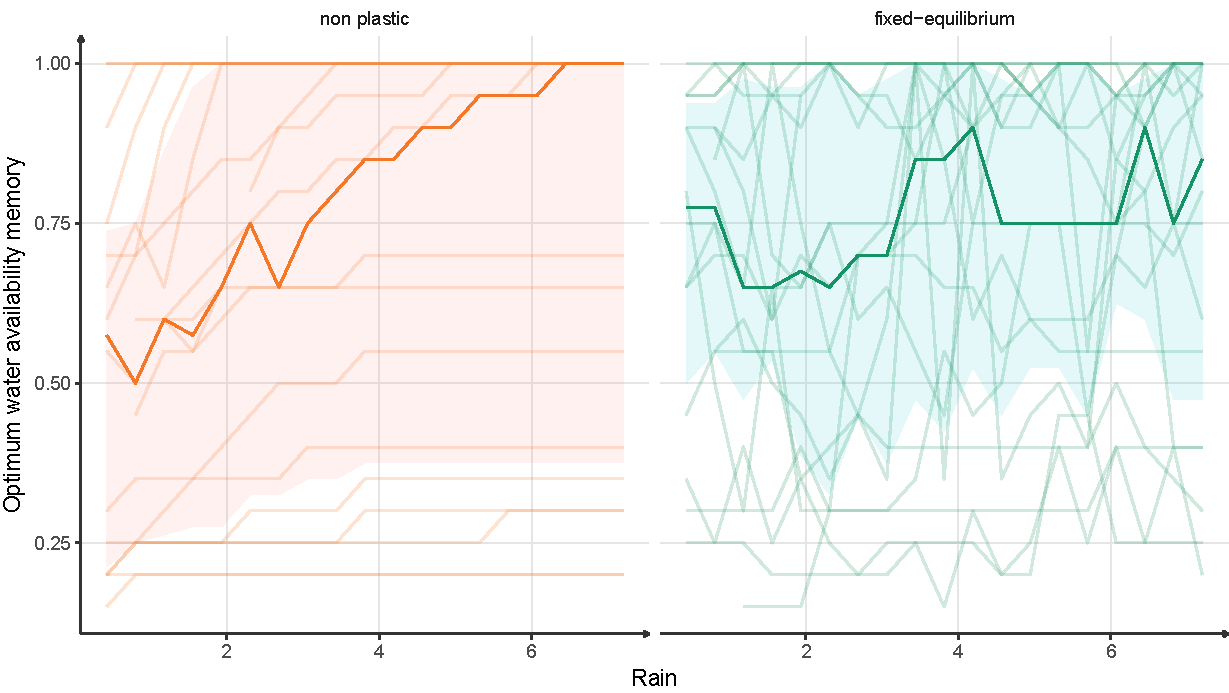
\includegraphics[width = \textwidth]{./2_PP/Figures/Rain/best_w_ini_pl_rain_grad_alt.pdf}
\caption{Median (dark line \textbf{-}) optimum water avaialbility memory along the water treatment gradient for \textcolor{myOrange}{- \textit{non plastic}} \&  \textcolor{myGreen}{- \textit{fixed-equilibrium}} allocation algorithms. The light lines (-) correspond to the 20 independent parameter sets. The color ribbon marks the band between the 5th and 95th percentiles.} % Maybe I should change that so it is the 25th and 75th like for variable inputs.
\end{figure}


\paragraph{Bigger productivity?}

The total cumulative biomass of all plants increases along the precipitation gradients. The plastic simulations have a cumulative biomass that is twice the biomass of \textit{non plastic} simulations.
%Strongly affect the potential overall productivity captured by cumulative biomass.


\begin{figure}\label{fig:total_BM}
    \classiccaptionstyle
\sidebysidecaption{0.60\textwidth}{0.3\textwidth}{%
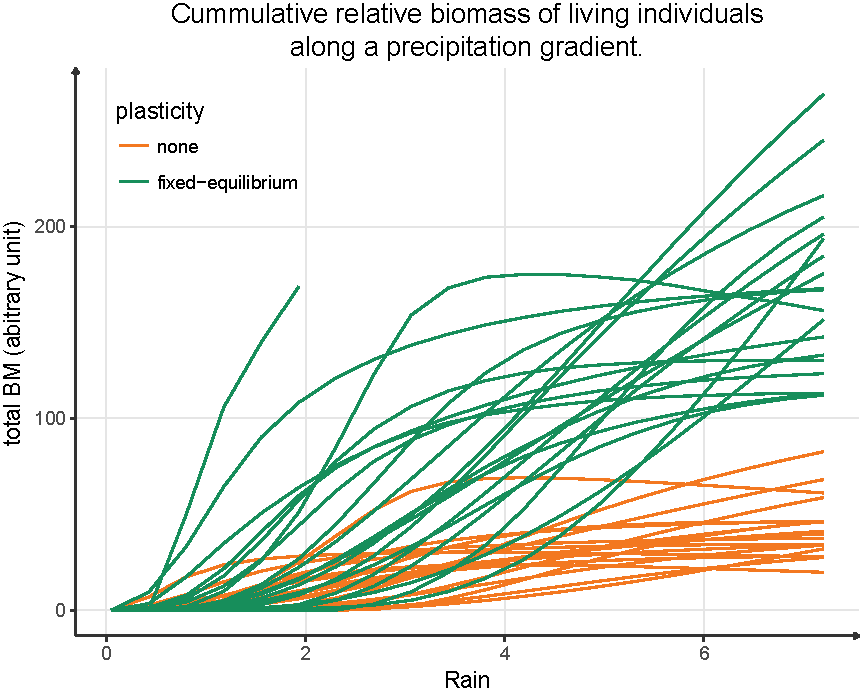
\includegraphics[width = \textwidth]{./2_PP/Figures/Rain/gradient_cumBM.pdf}
}{
\caption[Total biomass along a precipitation gradient]{Total biomass of all individual along a precipitation gradient for all tested parameter sets. Colour distinguishes plasticity treatments: \textcolor{myOrange}{- \textit{non plastic}} \&  \textcolor{myGreen}{- \textit{fixed-equilibrium}}.}
  }
\end{figure}

The effect on the maximum biomass is also investigated. For most simulation the maximum biomass is unchanged, and the median of the maximum biomass follow the same path for both conditions. However, the 75th and the 95th percentiles of plastic simulations shows a high increase in maximum biomass.
% But, only marginaly (for a few parameter sets) increases the biomass of best species.

\begin{figure}\label{fig:maximum_BM}
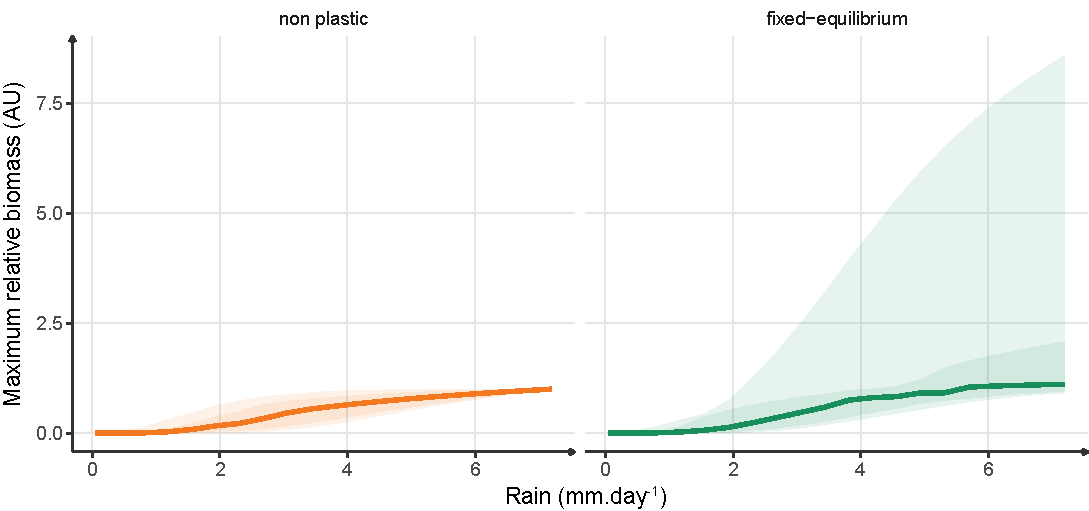
\includegraphics[width = \textwidth]{./2_PP/Figures/Rain/gradient_rel_BM_pl_trend.pdf}
\caption[Maximum biomass relative along a precipitation gradient]{Maximum biomass relative to the best performing plant in the most favourable condition for each parameter set, along a precipitation gradient.  Colour distinguishes plasticity treatments: \textcolor{myOrange}{- \textit{non plastic}} \&  \textcolor{myGreen}{- \textit{fixed-equilibrium}}.}
\end{figure}

%That probably means more species reaching high performance levels.

\paragraph{What about diversity?}

Similarly to the previous results, the potential diversity is estimated with the number of species, or the functional volume, of the species within the 90\%-100\% range of the maximum biomass for the given conditions.

\begin{figure}\label{fig:species_richness_grad}
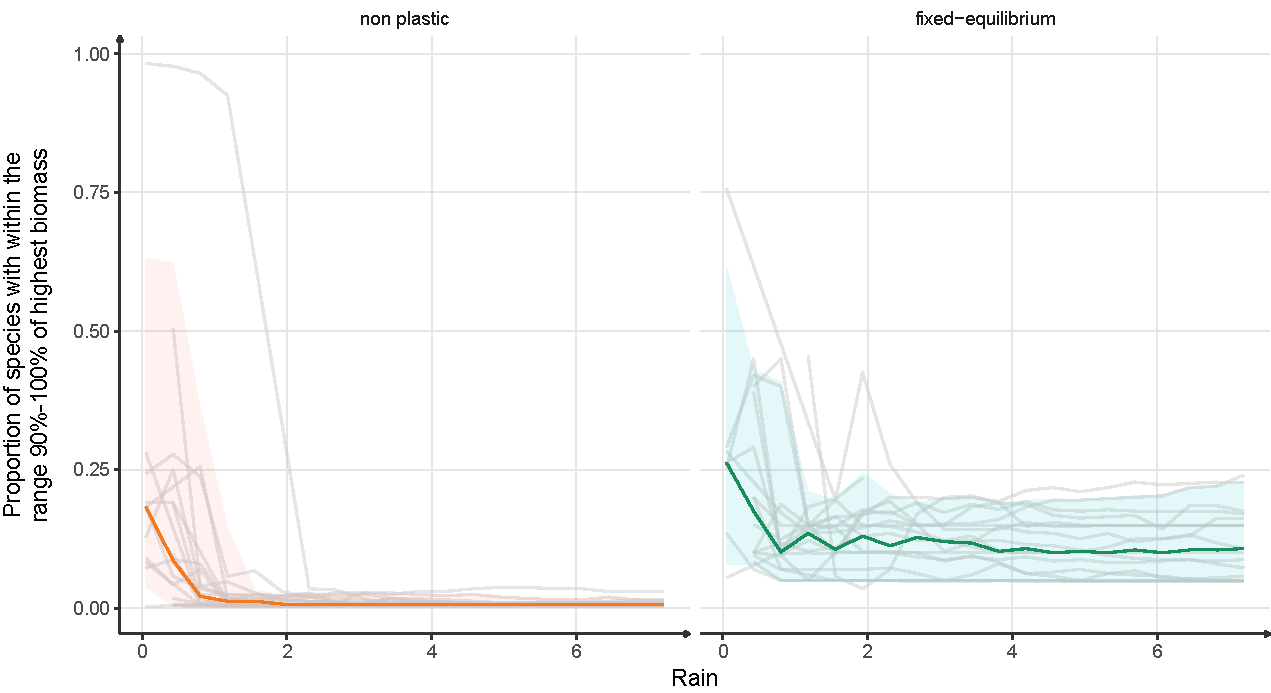
\includegraphics[width = \textwidth]{./2_PP/Figures/Rain/gradient_plot_spdiv10.pdf}
\caption[Species richness of the best performing species along a precipitation gradient]{Species richness of the species within the range 90\%-100\% of highest biomass for any given condition (parameter and precipitation) along a precipitation gradient.  Colour distinguishes plasticity treatments: \textcolor{myOrange}{- \textit{non plastic}} \&  \textcolor{myGreen}{- \textit{fixed-equilibrium}}.} \end{figure}

The species richness decreases along the gradient for the two plasticity treatments. The medians of species richness reach the low point for the same precipitation values than the medians of the optimum reach the highest values. The \textit{fixed-equilibrium} simulations show highest species richness along the whole gradient (except for one parameter set).

\begin{figure}\label{fig:functional_div_grad}
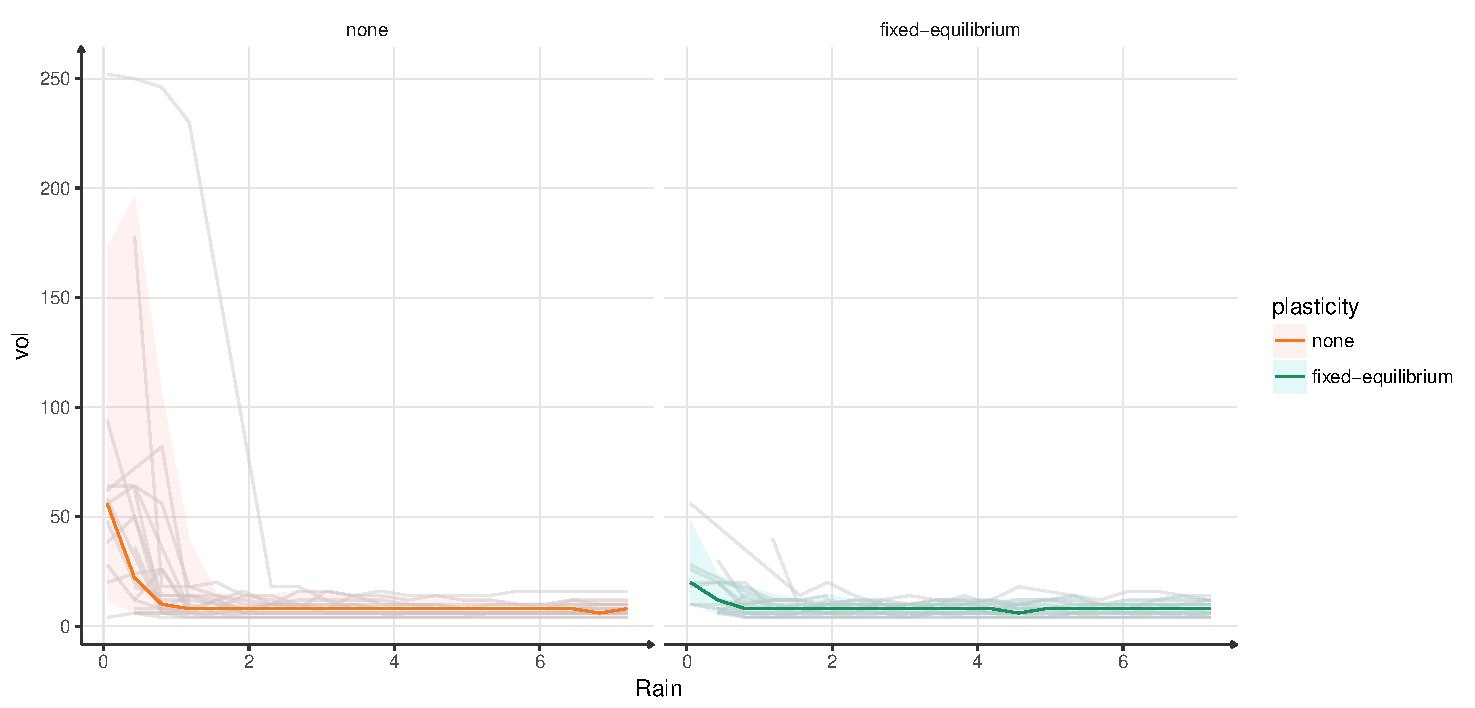
\includegraphics[width = \textwidth]{./2_PP/Figures/Rain/gradient_plot_fdiv10.pdf}
\caption[Functional diversity of the best performing species along a precipitation gradient]{Estimation of the functional volume occupied by the species within the range 90\%-100\% of highest biomass for any given condition (parameter and precipitation) along a precipitation gradient.  Colour distinguishes plasticity treatments: \textcolor{myOrange}{- \textit{non plastic}} \&  \textcolor{myGreen}{- \textit{fixed-equilibrium}}.} \end{figure}

The functional volume occupied by the top species, also decreases for both plasticity when the precipitations increase. For low watering values, the functional volume of \textit{non plastic} simulation is higher, however this difference disappear when both group of simulations reach low functional diversity.

\paragraph{Wider potential niches}

%A lot of effects discussed here emerge because a lot of different memories (equivalently RMF values) are associated to each resource use strategy for roots (shoot active tissue allocation being fixed and shared by all species). Another way of looking at the effect of plasticity focuses on only species identified as the best in at least one of the rain conditions. This focus reduces the number of species to species selected along such gradient and allow to ignore species that would not be present anyway. This selection does not take into account any competitive mechanisms that could change the identity of the dominant species in a given condition. Nevertheless, information on how the relative performance of theses species can still be collected.

%The potential effect of plasticity on niche breadth is visualised here for one representative parameter set.
The median performance of the best performing phenotypes for each conditions of the gradient are compared with and without RMF plasticity (\textit{fixed-equilibrium}) along the gradient. It is limited to the best phenotypes to mimic a degree of biotic filtering. The plasticity greatly enhance the ability of the plants to maintain a high growth, often comparable to the one of the best phenotype, along the gradient. The extreme low value of the gradient show no differences between phenotypes because the water level does not allow plant to grow, only the organic matter contain is the seed is used, leading to similar outputs. As seen in figure \ref{fig:gradient_strat_trend}, the best phenotypes often share the same strategy, but differ in memory for resource availability (figure \ref{fig:gradient_strat_trend}). Under \textit{fixed-equilibrium} allocation (right panel), the left end of the gradient (except the first value of precipitation) shows more contrast in the performances in strategies, while the righ end (more water) shows very little contrast. This is very different from the \textit{non plastic} allocation results (left panel) that show large differences between the best strategies along the whole gradient.  

\begin{figure}\label{fig:gradient_ranking}
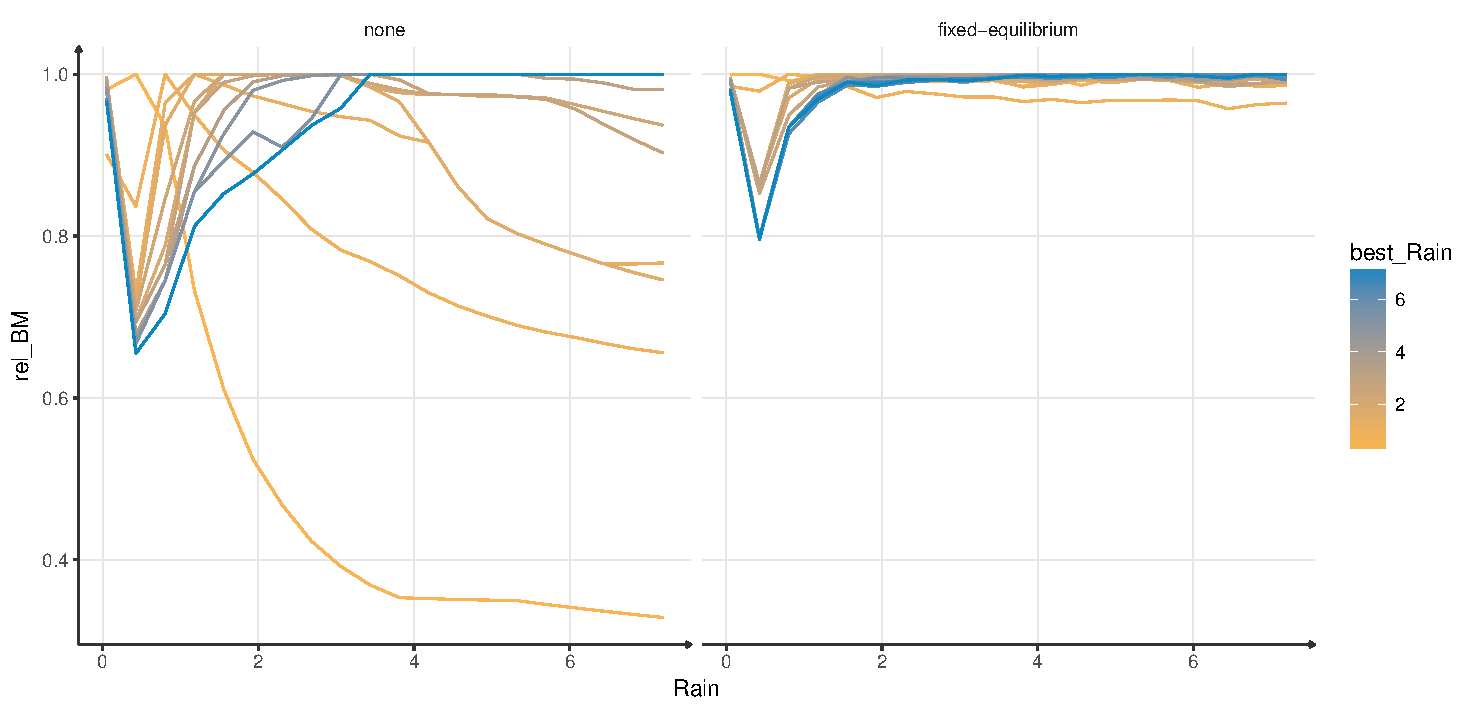
\includegraphics[width = \textwidth]{./2_PP/Figures/Rain/optimum_shifting_median.pdf}
\caption{Median relative performance of best phenotypes along a precipitation gradient for 20 parameter sets.}
\end{figure}

%The effect of the plasticity on the potential niche can be observed by looking at the cumulative number of species within the 91\%-100\% range of maximum biomass along the gradient (figure \ref{fig:gradient_ranges}). For all parameter sets, there is an increase in the number of species 
%
%
%\begin{figure}\label{fig:gradient_ranges}
%\includegraphics[width = \textwidth]{./2_PP/Figures/Rain/gradient_range_nb_sp.pdf}
%\caption[Changes the dominance structure]{Changes in the dominance structure for the evaluated parameter sets. The dominance structure is illustrated by the cumulative number of species along diminnishing number of conditions where they are within the top 90\%-100\% range of highest biomass for any given condition. }
%\end{figure}




\subsection{Discussion: gradient of homogeneous conditions}

\paragraph{Strategy shift}
Along the watering gradient, the optimum strategy (active tissue allocation in roots) changes from conservative toward exploitative. This shift demonstrates that the trade-off between active and structural tissues allocation allows different strategy to dominate in constrasting conditions \parencite{wright_worldwide_2006}. This shift occurs for low values of the gradient and exploitative strategies are dominant over a large part of this gradient. This can be explained by high precipitation values disconnected from the precipitation values observed in nature. Also, the low resolution of the strategies (15 values for the proportion of active tissues in roots) limits the possible number of different dominant strategies along such gradient. 

%\paragraph{Static and dynamic gain}
%\paragraph{Who benefit from plasticity}
%
%Gains from the plasticity can be distinguished between static and dynamic gains. The lower value of the \textit{center of gravity} in conditions of low water availability under \textit{fixed-e"quilibrium} algorithm seems to indicate that conservative strategies benefit from plastic allocation more than exploitative species. However, this effect is mostly due to static gain as the optimum strategy does not change. This effect is due to a growth landscape flatter than in better conditions (more species within the 90-100 \% of maximum growth, lower growth difference with best strategy) and asymmetric, that has two effects:
%\begin{itemize}
%\item it reduces the growth gain for species with strategy close to the optimum, but not at the equilibrium (figure \ref{fig:optimum_shift} panel A);
%\item increases the potential gain (relative to less flat growth landscape) for species with strategies more conservative than the optimum (figure \ref{fig:optimum_shift} panel A).
%\end{itemize}

\paragraph{Static gain}

% static gain idea
While the cumulative productivity of all species combined is largely improved by the plasticity for all parameter sets (see figure \ref{fig:total_BM}). However, the best total biomass is only improved for a fraction of these parameter sets (see figure \ref{fig:maximum_BM}). This observation supports the idea that the total biomass is mostly increased due to an improvement of plants with a non optimum phenotype. These 

% convergence idea
Moreover, while the number of species reaching high performance levels increases with plasticity (corroborating the previous conclusion), the functional diversity does not increases. We can conclude that the phenotypic plasticity leads to a convergence of the plants toward good performance phenotypes. Therefore, the productivity gain provided by the plasticity comes mainly from the convergence toward the best fixed phenotype, and cumulative static gain. This mechanisms does not consistently support functional diversity of the vegetative traits, but it can increase functional redundancy. The species diversity can be increased by this form of gain, and it may limit the the vulnerability of the community if multiple species have the function.

% other dimensions diveristy
The functional convergence is obvious when only the vegetative dimensions are observed. But the functional diversity may be considered for other traits, therefore the promotion of species richness by the reduction of fitness differences can promote the functional diversity of the community. 


\paragraph{Niche widening}

The phenotypic plasticity of the RMF leads to an important widening of the potential niche. This is explained by the removal of one constraint of the niche. Indeed, with cost-free plasticity in RMF, the equilibrium is almost guaranteed for all species and the resource-use strategy is the only limitation of a species niche. Because the best proportion of active tissues is the same for a long portion of the gradient (high water availability)(see figure \ref{fig:gradient_strat_trend}), along the gradient most of best phenotypes share this resource-use strategy. Therefore, along this same gradient, if the RMF axis is ignored, the different species have equivalent phenotypes (except for a few first growing  days).

This niche widening has for consequence a higher niche overlapping. This overlapping can be translated into lower niche differences, as the niche are now discrimated only on one dimension, and into lower fitness differences as the species with similar strategies but different memories have close performances under plastic allocation. According to \cite{turcotte_phenotypic_2016} these two processes have opposed effects (see figure \ref{fig:plasticity-effect} in chapter \ref{part:literature}). The reduction of the niche differences diminishes the positive effect of heterogeneity on diversity, while the reduction of fitness differences reduces the competitive exclusion of the non dominant species. The current simulations do not allow to tell which effect will be the strongest at the community scale. The cost of plasticity should nevertheless ensure some degree of niche differentiation. However, in addition to these two effects, the widening of the potential niche corresponds to a reduction of the abiotic filtering pressure, and should promote the diversity as more species can potentially invade an habitat. 

\paragraph{Competition effect}

The reduction of the abiotic filtering suggests an increase in the biotic filtering due to the limited carrying capacity of the habitat. This could increase the competition intensity at the beginning of the growing season, and eventually change the dominant species if this increase is strong enough to alter the competition outcome toward more competitive species. Unless the eventual new dominant species has a dramatic effect of the overall productivity or diversity, the effect of the phenotypic plasticity should be positive or null on these properties. The phenotypic plasticity does not alter directly the optimum phenotype in temporally fixed conditions, therefore the impact on the competition outcome should be limited.

\paragraph{Meta-community dynamics}

While the effects at the community level are still hard to defined, the phenotypic plasticity can alter the dynamic at the meta-community scale. Phenotypic plasticity, by reducing the abiotic filtering effect, allows for stronger link between the communities as the chance to transfer from one community to another are higher. Therefore this mechanism has a positive effect on the stability of the ecosystem as species from unperturbed communities can invade, and partly sustain the properties and services of the perturbed community.

In the context of the global change, to survive two options are possible: (1) migrate to new habitat with suited conditions, (2) adapt to new condition in the same habitat. In this context, the phenotypic plasticity facilitates both the adaptation to new conditions in the same spatial habitat and the adaptation to a new habitat that match the ideal conditions only to a certain degree. By facilitating the adaptation to new conditions or habitat, the phenotypic plasticity reduces the relative importance of climatic variables compared to the competition as already suggested by empirical results \parencite{alexander_novel_2015}.

%
%This widening is, however, asymmetric because there is a transition of the limitations that define a species niche. Without plasticity, in a given homogeneous environment, the optimum phenotype is defined by both the adequate resource-use strategy and the balance between organs. With costless  Conservative species are less efficient in high resource availability conditions, while exploitative species are more efficient. 
 
% If cost are low, the effect is likely to reduce potential species diversity. An established species can, thanks to static gain, maintain relatively high growth rate in an habitat where the balance is different but the optimum strategies closed. This is particularly true for rich environment where the optimum strategy for roots is quite stable. The effect on coexistence is better illustrated with an example. Given two species, \textit{species a} and \textit{species b}, with optimum strategy (PAR) and RMF for two distinct conditions, respectivelly \textit{A} and \textit{B}, in a heterogeneous environment composed of majoritarely condition \textit{A} and minorly condition \textit{B}, ... where do I go with that ? ... 
 


%Reduce the structural role of spatial heterogeneity. Favour seed dispersal strategies. In high resource conditions, the resource levels do not matter much (non linearity of the optimum along gradient) but balance does, plasticity could reduce species richness, unless cost of plasticity. Unless not enough space to really be a niche (rare conditions): give opportunity to some species to extend their niche.

%\paragraph{Fitness evenness}
%
%The phenotypic plasticity reduces the importance of the filtering effect of abiotic conditions by increasing the flexibility of one of the niche axis (the balance between shoot and root activities). This increase in growth evenness between species will certainly impact the community properties. Multiple effects can be anticipated on the mechanisms that affect these properties. The first effect
%
% 
% However, what is the effect on coexistence mechanisms. The widdening of the potential niche of numerous species, Probably negative: so hard to tell effect on coexistence.


\begin{figure}\label{fig:rain_pl_effect}
    \classiccaptionstyle
\sidebysidecaption{0.60\textwidth}{0.3\textwidth}{%
\includegraphics[width = \textwidth]{./2_PP/Figures/Rain/rain_pl_effects.pdf}
}{
\caption[Effect of plasticity in constant conditions]{Effect of the phenotypic plasticity on the main properties of the grassland communities in constant conditions.}
}
\end{figure}

\textbf{In constant environmental conditions, the phenotypic plasticity already has an impact on species performances and interactions through the static gain it provides to species wit the good resource-use strategy. It increases the fitness evenness of species by reducing the abiotic filtering dimensionality. This leads to a convergence of the phenotypes and a widening of the potential niche. The effects at the community level are hard to anticipate, but they will be largely dependent on the competitive interactions and how they are affected by the plasticity. The reduction of the abiotic filtering will likely increase the species diversity, but the functional diversity might not follow this trend due to functional convergence. The effects on the other component of the ecosystem properties cannot be fully determined and greatly depend on the outcome of the competitive interactions. In temporally heterogeneous conditions, the phenotypic plasticity may play a larger role and greatly mediate the inter-specific interactions. }


%\textbf{Mostly static gain, but even if there is gain, increases the potential niche of species that are settled. Bigger niche: favourable for conservative species of rare habitats.\\
%Hard to tell anything on coexistence, except wider niches}



\subsection{Results: gradient of heterogeneous precipitation conditions}

This part of the chapter present the results at the individual scale along a gradient of temporal increasing variability of the underground resource (increasing negative slope of water influx).

\paragraph{Productivity}
The maximum biomass (relative to the \textit{non plastic} best performance in constant watering conditions) decreases along the gradient for all allocation algorithms (see figure \ref{fig:variable_BM}). The \textit{non plastic} algorithm show a drastic drop after the fourth level of variation, while the fixed-trait algorithms show better performances in this part of the gradient. The \textit{plastic-optimisation} algorithm show low growth for all conditions, but a more stable performance.

In contrast with the stable conditions (see previous results) the plasticity provide, in non constant conditions an great improve in the maximum biomass for most parameter sets. 

\begin{figure}\label{fig:variable_BM}
\includegraphics[width = \textwidth]{./2_PP/Figures/Variable/var_relnone_BM_trend.pdf}
\caption[Biomass variations along a gradient of resource variability]{Biomass variation of the best performing species along a gradient of resource variability for four plasticity treatment. The upper panel of the top-left frame illustrate the water influx as a function of time along the variability gradient. The dotted lines in the top-left frame indicate the median biomass for the other three algorithms. }
\end{figure}

%
%Along the temporal heterogeneity gradient the median biomass of the optimum phenotypes decreases under all allocation algorithms when the variability increases despite the same mean water influx. The amplitude of reduction varies with the allocation mechanism: \textit{non plastic} algorithm shows the largest decrease while \textit{fixed traits} algorithms show slower decrease. \textit{Plastic- optimisation} simulations have more constant performances with low initial performances in constant condition (between 5\% and 55\% on the \textit{non plastic} simulation), but they end with slightly better performances than \textit{non plastic} simulation for the extreme case of variation (two extreme regimes).

\paragraph{Identity}

In addition to a reduction of biomass, the increasing slope of the water influx reduction lead to a shift of the optimum strategy in \textit{non plastic} simulations (see figures \ref{fig:variable_strategy} \&  \ref{fig:variable_trajectories}) toward more conservative strategies. The median optimum value shifts from 0.85 to 0.75 then 0.35 in extrem conditions. This reduction of optimum toward more conservative strategies is offset in most of \textit{fixed-equilibrium} and \textit{fixed-optimisation} simulations where the median optimum value for the PAR stays above 80\%. Only a small reduction (around 25\%) of the 5th and 25th percentiles of the optimum root strategy can be observed between the extreme conditions for these two algorithms.

\begin{figure}\label{fig:variable_strategy}
\includegraphics[width = \textwidth]{./2_PP/Figures/Variable/var_strat_trend.pdf}
\caption[Strategy shift along a gradient of resource variability]{Strategy (PAR: proportion of active tissues in root) shift of the best performing species along a gradient of resource variability for four plasticity treatment. The dotted lines in the top-left frame indicate the median PAR for the other three algorithms.}
\end{figure}

 This shift in optimum strategy can better be observed on the plan of the proportion of active tissues in root (PAR) and root mass fraction (RMF) in figure \ref{fig:variable_trajectories} where all trajectories\sidenote{trajectory of the optimum, not of the species.} along the variability gradient are plotted. \textit{Non plastic} allocation trajectories by a linear shift toward more conservative strategies with higher allocation to roots, while \textit{fixed-equilibrium} and \textit{fixed-optimisation} trajectories are non linear and can be divided into two phases: (1) increase in RMF, (2) reduction of PAR. \textit{Plastic-optimisation} algorithm shows no consistent pattern in trajectories.


\begin{figure}\label{fig:variable_trajectories}
\includegraphics[width = \textwidth]{./2_PP/Figures/Variable/var_2D_strat_dyn.pdf}
\caption[Best phenotypes along water resource variability gradient]{Best phenotypes along water resource variability gradient. Thinner lighter lines indicate low water variability, while the thicker lines indicate strong temporal heterogeneity.}
\end{figure}

\paragraph{Diversity}

%As previously seen, plasticity can affect diversity in a drastic way, reducing the functional diversity by contracting the phenotypic space, but also increasing the potential species diversity by the same mechanism. The effect of static gain\sidenote{refers to the gain due to convergence toward a good static phenotype and no temporal changes.} and dynamic gain must be disentangle. The 


Along the gradient, the performance and the identity of the bet phenotype were greatly altered by the water variability, but the phenotypic plasticity mitigate these effects. The number of species is fairly stable for all alogrithms but the \textit{non plastic} that show an improvement in species diversity. The fixed allocation algorithm have between 15\% \& 20\% of the species within the 90\%-100\% range of the maximum biomass for the conditions, while the \textit{non plastic} allocation show this level only of the extreme variable case, but otherwise is limited to a few percents. The functional diversity is stable along the gradient and is similar for all agorithm (\textit{plastic-optimisation} algorithm being exclude)(data not shown).

\begin{figure}\label{fig:variable}
\includegraphics[width = \textwidth]{./2_PP/Figures/Variable/var_spdiv_trend.pdf}
\caption[Species richness of the best performing species along a water resource variability gradient]{Species richness of the species within the range 90\%-100\% of highest biomass for any given condition (parameter and precipitation) along a water resource variability gradient.  Colour distinguishes plasticity treatments: \textcolor{myOrange}{- \textit{non plastic}} \&  \textcolor{myGreen}{- \textit{fixed-equilibrium}}.}
\end{figure}

%Changes in optimum, but does it affect eveness ? Same pattern as before with tehe trade-off between species and functional diversity. What happen if you filter down stuff ?





\subsection{Discussion: gradient of temporal variations}

\paragraph{Resistance to variability}

Before analysing the effect of the different plastic algorithm, the \textit{non plastic} simulations show interesting patterns. The first thing inform us on the relative importance of growing versus surviving. Because the mean water influx over the simulated period is conserved, an increase in the influx negative slope means that during the first half the plants have more available water, while they have less during the second half (relative to constant influx. The decreasing biomass along the gradient suggests that this additional water (and therefore potential growth) does not compensate for a reduction in growth during the drought period. Therefore, it is more important for the plant fitness to limit losses during scarce period instead of maximizing growth during favourable periods. 

\begin{marginfigure}
\includegraphics[scale=1]{./2_PP/Figures/Variable/GalanthusNivalis.png}
\caption[\textit{Galanthus nivalis}]{\textit{Galanthus nivalis} is an example of species that develop early in the season to avoid competition and benefit from the high resource availability.}
\end{marginfigure}

However, this conclusion should be mitigated by the fact that some reproduction strategy still can benefit from early exploitative strategies and there are not considered here because the success is measure by the biomass afeter 100 days. This effect can be explained by the fact that even the most exploitative species are not fully developed when the resources are the most available, therefore the potential compensation by an early growth is limited. This is the case in the context of mountain grasslands, and some specific life cycle strategies take advantage of this particularity like the \textit{galanthus} species (see figure \ref{fig:galanthus}) with early development\parencite{schroder_modelling_2014}, or development from bulb that allows for an early and rapid growth.

% selection of more conservative species, plus reduction of prod that show non compensation mech. -> best strategy during the bad period, but no
%The selection of more conservative strategy at the end of the gradient confirms the importance of maintaining growth (or reducing losses) during the period of lower water availability, and demonstrates the higher resistance of the conservative strategy to the resource fluctuations.
The reduction of biomass along the gradient, even in plastic conditions, supports the idea of a lack of compensation mechanisms between favourable and unfavourable drought periods. In addition to this conclusion, the better performances of the conservative species in low water conditions relative to exploitive species (see figure \ref{fig:gradient_strat_trend}), suggests that the best strategy is determined by the optimum resource-use strategy of the most important growth period (the drought period). However, another mechanism can be involved and is relative to the capacity of the species to perform well both in conditions that suit its phenotypes, and in conditions that do not suit its phenotype. In a variable environment, the phenotype does not match conditions different from its niche center because of the optimum resource-use strategy may change, or because the balance between root and shoot activity changes. Both can be important. As said, the former is suggested by previous results, however under plastic allocation the optimum resource-use strategy is maintained at high values of proportion of active tissues. Therefore, the difference in optimum resource-use strategy along the gradient cannot explain alone why conservative strategy are better in contrasted environment. The other explaining mechanism is a better resistance to variability from conservative species, relative to exploitative. The variability in water conditions while the light conditions are fairly constant leads to a shift in the balance in the availability of the two resources. If the phenotype is fixed, a shift from balanced conditions (equilibrium between shoot and root is respected for the given phenotype in these conditions) to unbalanced conditions (no more equilibrium for the same given phenotype) can be seen from the plant perspective as a reduction of the overall gain function stronger than the actual decrease in resource, because the non limiting organ is in over-capacity. Therefore, to the given plant, the decrease in resource is stronger than the actual decrease in resource, and the resource-use strategy shift towards a more conservative strategy than a balanced phenotype would require.

% message: it is not because the optimum change, it is because the conservative species are more resistant to variability.


\begin{figure}
\includegraphics[width = \textwidth]{./2_PP/Figures/Variable/explain_assymetry.pdf}
\caption[Assymetric gain from gains and costs perspective]{Gain and lost curves along the allocation strategy axis for one organ. Left panel corresponds to the gain and cost in a situation where the equilibrium is maintained, the right panel illustrates the effect of a 30\% loss of gain due to unbalanced exchanges between organs. The botton bar plots represent the net gain of two distinct phenotype in the two conditions.}\label{fig:assymetric_gain}
\end{figure}

\paragraph{Who benefit from the plasticity?}
% who wins -> assymetric and impact of the identity
While the phenotypic plasticity does not provide any clear advantage to a type of species in constant conditions, in changing conditions the phenotypic plasticity benefit to the exploitative species that are able to maintain good performances in contrasted conditions (see figure \ref{fig:variable_strategy}). Because the plasticity gain is assymetric, the phenotypic plasticity alters the identity of the community and promotes exploitative species in variable conditions while conservative species are favoured under \textit{non plastic} allocation. In a more theoretical view, the plasticity can be seen as an alteration of the strength of the stress as shapping factor of community \parencite{grime_evidence_1977}. If the plasticity allows the exploitative species to better support stress, in modelling studies that do not take into account such plasticity, the amplitude of the stress needed to see a shift in the community identity may under-estimated.

% Why is that ? absolute and relative, the role of the euilibrium

%Because the shift in non plastic condition is due to vulnerability, and not optimum strat during the most growing period. (there could be some compensation, leading to best exploit phen,, even if conservative are indeed more perf in drought period).

% What what consequences for the productivity (cite maire)




\paragraph{About diversity}


\paragraph{Improvement in variable conditions}
Plasticity has a a positive effect on exploitative strategies in low resource availability conditions. As said earlier in the document, plant performance depends on multiple things: the effectiveness of organs, the global resource availability and the equilibrium. 
% Here talk about the spatail heterogeneity:
If plasticity improve the performance of the exploitative species, it is unlikely to be because of the contraction of the space since it is the optimum only that is looked at. Also means it is probably dynamic gain, it the filter was static, plasticity shouldn't have change much. And there is gain, even in the high end of the gradient where the optimum does not move, saying that the optimum is fairly conserved despite increase in resource (but low resolution of the strategy space, and match the function). 

% From theere, talk about the variable rain input.
Change in optimum strategy can be explained by: an assymmetry in efficiency (better a but more conservative in exploitative favourable conditions than exploitative in conservative favourable conditions) or an assymetry in inbalance cost (better be inbalanced when conservative than when exploitative). The first option is not consistent with previous results (see subsection \ref{section:landscape}, figures ...) that show higher fitness for species more exploitative than the optimum, compared to species more conservative. In the other hand, following results show positive effect of functional equilibrium over conservative strategies. Nevertheless, this effect certainly results from an artefact and the contraction of the phenotypic space not in favour of exploitative strategies. The sensitivity of exploitative strategies to low conditions is visible in figure \ref{fig:gradient_optimum_strat}

Shift of RMF then strategy explain quite well that the equilibrium is more important than the resource usage and the organ efficiency. How does that inform us on the real world ?

 - potentially reduces the meta community diversity if spatial heterogeneity has a less drastic effect on strategic dominance. - talk about that in diversity part

/!\\ may come from a lack of coordination with shoot. Since shoot activity is suppose to be relatively high. == might not have besn a good choice to look only at root strategy. But, since there is adjustment of RMF that allow to maintain equilibrium and resource usage, it should be fine to interpret these results.

\textbf{Phenotypic plasticity give exploitative species an advantage in variable conditions because their growth rate rely more on productivity and therefore equilibrium than conservative species. }

% Indirect effect of identity on diversity, mention it but more a perspective.

%\paragraph{Heterogeneity of response}
%
%Kichenin (different response to gradient) Doesn't work in this framework: Not so sure about that: depending on your initial memory plants show directional changes toward one phenotype. Yeah, but they should have converged for other conditions too... So, it doesn't work. Might be explained by:
%\begin{itemize}
%\item different conditions: because heterogeneity and habitat selection, or changes in competition hierarchy;
%\item different ways to tackle changes on one dimensions;
%\item different weights between mechanisms impacting composite traits, because of the different traits.
%\end{itemize}


\begin{figure}\label{fig:variable_pl_effect}
    \classiccaptionstyle
\sidebysidecaption{0.60\textwidth}{0.3\textwidth}{%
\includegraphics[width = \textwidth]{./2_PP/Figures/Variable/variable_pl_effects.pdf}
}{
\caption[Effect of plasticity in variable conditions]{Effect of the phenotypic plasticity on the main properties of the grassland communities in variable conditions.}
}
\end{figure}


\textbf{The phenotypic plasticity implemented in \model improve the relative performance of multiple strategies by concentrating the plant toward a subspace of higher performance for most of plants. Convergence to a smaller subspace can be assimilated to reduction in phenotypic diversity, but it reduce performance heterogeneity and should favour local plant diversity. However, this effect should be limited by plasticity cost. Indeed, if the growth gain due to plasticity is only static, any species with a fixed phenotype closer to the optimum than the focus species has a better growth rate and exclude the focus species.
. a few words on dynamics... Meta-community diversity is however reduces by the reduction of potential axis for niche differentiation. Plasticity costs and limits should play major role in the balance between these mechanisms. Community level simulations are needed to further understand the cumulative role of competition, spatial and temporal variability and plasticity costs on phenotypic plasticity influence on plant community dynamics.}


\section{From model behaviour to competition and coexistence in the real world}*

% ! ! ! 
% Talk about how the model informs on the effect of plasticity:
% do not really mimic the reality since the plasticity can be turn on and off, but when there is an effect, it tells us how to modulates the other effects (stronger if opposite, or less strong if in the same direction), and help us identify the real sources and amplitude of effect.
% Nevertheless, could it not tell us how real plasticity impact communities when there are evidences of plastic vs non plastic plants... ?

\subsection{Plasticity: new functional diversity}

functional diversity of plastic traits? Should them be excluded?

Impact of traits, and abundances: the need to account for it!

May still be useful especially for invasion, and works well despite low flexibility (see \parencite{forsman_rethinking_2014}. May allow more diversity if some correlations with other non plastic traits.	

\subsection{Plasticity as a strategy: cost and correlations}

\paragraph{Who benefit from plasticity?}

\paragraph{Cost of plasticity}

and limits ? what about exhaustion

\paragraph{Plasticity as a strategy}
One of the argument to say this is new, however not really explored, neither with plasticity cost perspectives (a bit with plasticity limits) or with tau. However, used extreme cases: give better understanding and necessary before finer analysis. Still, there are hypothesis on the effect on diversity and the role in phenotypic stability (attention: isn't it just because the formulation of projection is wrong that we can make these conclusions ?).



\subsection{Plasticity and competition: changes in interactions}

\paragraph{Extended interpretations}
What about the continuous $\tau$ gradient ?\\

What about interactions and cycles ? Little has been discussed on the dynamic of the resource and how it could affect coexistence. Imagine that with cycle, reproduction timing has an importance here...


plasticity will change: performance, sensitivity and impact of the resource.

%\section{From individual response to community dynamics}

% Use these notes to extend the discussion and add some outlooks
%
%\section{Niche response}
%
%
%Obj1: understand how resource use mechanisms and allocation algorithms shape the environmental potential niche in the context of the model.\\
%H1: strategy and memory affect niche in two ways if we suppose they are independent: shape and position. Strategy mostly affect shape (width and height) while memory (and so root:shoot ratio) affect mostly position.\\
%H1': there is strong link between strategy and memory in the case of optimisation allocation that increase niche height and might reduce its width.\\
%Obj2: understand the role of plasticity on the niche and if the effect in the same for all strategies/memories.\\
%H2: the plasticity increase niche width but not height (as phenotype is optimum at the center of the niche where memory match the resource availability).
%
%Stability and efficiency trade-off. Niche heigh and width and relationship with the strategy. How does plasticity affect that ? Does it increase the height and widen niches ? What does that mean for coexistence ?\\
%Hopefully higher niche would go with unstable niche.
%%
%%\section{Transitivity and competition}
%%1 vs 1 interactions\\
%%Is the resource competition transitive ? How does niche widening impact that, does plasticty change competition interaction. Is it related to the trait distance ? (don't think so)

%
%\chapter{The effect of phenotypic plasticity on plant community dynamics}
%Hypothesis on the cumulative effect on niche and interactions.
%
%\section{Individual resistance and resilience against drought events}
%Amplitude and length of the event :\\
%- severity effect reduced by lower tau ?\\
%- resistance versus resilience: H0: conservative strategy have higher resistance, H1 : low tau allows for re-equilibrium and increase resistance (low amplitude and long length. H2: high tau allow to avoid dead-end situation during short severe drought (high resilience)
%\section{Community response to drought event}
%coexistence effect vs resistance/resilience effect\\
%uniform vs heterogenous (plasticity wise) community response
%H1: 
%

\chapter{Community level parametrisation}

\section{Method}

\paragraph{Field calibration}
New random parameters sets (with no species specific parameters) for population dynamics and competition specific parameters (see table ...).
Sequence of around 60 year for each site. Parameters were selected by...


\paragraph{Field data}
Field data has been collected between years 201 .. and 201 by Claire Deleglise and al. ().

\paragraph{Weather data}
Weather data has be computed by the MeteoFrance model SAFRAN by ... using GPS coordinates and slope, azimuth and horizon computed from a "MNT". These parameters were also used by the model CROCUS to compute snow accumulation and melting. These high frequency data (resolution under 1h) have been average daily and used to compute input variables for \model . 

\section{Results}

\chapter{Plasticity: impact on species fitness and diversity}

\section{Method}

\section{Results}
\subsection{Plasticity: a winning strategy ?}

\subsection{Effect on coexistence}

%
\begin{fullwidth}
This short final chapter summarises the main results and advances produced during this PhD. It is also the opportunity to look ahead and trace future directions to extend upon this work. Imagining extensions to implement and questions to explore is an infinite game, and while many developments are proposed, I try to keep this discussion succinct and close to the current state of the model.
%While researchers are prone to imagine many developments and follow exiting ideas, I try here to be succinct and to consider only a few of the many paths we could follow to extend the model and progress in the field of community ecology.
\end{fullwidth}

%_________________________________________________________________________________
\chapter{Synthesis}
%
%Point out the novelty, acheived work 
%
%begin to fill the gaps of community dynamics: \parencite{berger_competition_2008}: effect on local environment, adaptive behaviour and below-ground.
%
%Pllus: lack of diversity.
\section{A new agent-based model of mountain grasslands}

The implementation of the model \model was the opportunity to develop a new framework from scratch to tackle unresolved scientific questions. Thanks to the freedom that was given to me, I could approach the project in a personal way, developing concepts, accumulating ideas, and developing a (too) complex model of grassland communities.

\paragraph{Filling the gap}

The model developed had the ambition to fill the gap between fine-scale agent-based models, integrating physiological processes, fine-scale resource dynamics and phenotypic plasticity with large-scale community dynamics model, long-term dynamics of numerous species in a heterogeneous environment. Filling this gap is necessary to better understand and predict the dynamics of natural (and semi-natural) systems in the context of the global change, affecting both the climatic conditions and the management scenarios. On one hand, fine-scale models were not capable to be deployed at large scales to integrate the effects at the local-scale to the global system. On the other hand, the large-scale community dynamic models overlooked some fine-scale processes such as the intra-specific variability, and in particular the phenotypic plasticity. Better integrating these two levels can help us better predict changes in the main properties of the grassland communities, and the effect on the ecosystem services.

\model manages to fill this gap by integrating the plant functioning and the phenotypic plasticity into a framework based on the leaf economic spectrum and developed around strategic allocation trade-offs. The partitioned allocation to the active and structural tissues regulates the balance between resource exchanges and respiration and tissue turn-over costs. These trade-offs allow a coherent representation of the plant functioning while drawing a closed strategy space where the diversity of plant species can be modelled. This strategy space, at the core of the model, is also at the centre of the phenotypic plasticity conceptual framework developed in this work. The phenotypic axes drawn by the trade-off offers a space in which plant can evolve \sidenote{not in an evolutionary perspective, yet.} based on their projection of the external conditions. This projection is the engine that drives the phenotypic plasticity and allows the modelling of a strategic plasticity, that contrasts with ubiquitous plasticity. The implementation of multiple rules to drive this plasticity allows to better understand this mechanism of phenotypic plasticity and to test the robustness of the observed patterns.


\paragraph{Consistency}

While the steps of parametrisation highlight some progress to make in the implementation of the phenotypic plasticity, the current version of \model offers stable growth, both at the individual level and the community level, and a strong tool to start exploring the effect of the phenotypic plasticity. This stability is supported by the consistency of the results between the numerous observed parameter sets. Despite the difficulty to reproduce some specific empirical patterns, the plasticity improves the performance of the model and impacts its behaviour, encouraging us to further explore its effects at the individual scale first, then at the community scale.

\paragraph{Strategies and performances}

The strategy space build with independent strategy axes allows the modelling of a multitude of species. While the diversity offered by this new framework is not fully explored and used, the vegetative dimensions are extensively analysed. Because there are based on strong) empirical trade-off, these dimensions draw a wide performance landscape that (1) have the potential for high functional richness, (2) evolve as a function of the resource levels. Better integrate this landscape in the plasticity mechanisms will be key to better represent the phenotypic plasticity. This analysis also identifies the root mass fraction (RMF) dimension as a key trait to control the plants' performances, and therefore support the investigation of this axis as a plastic dimension.


\section{A better understanding of the effects of plasticity}

The multiple plastic allocation algorithms, with varying plastic dimensions (RMF only, or in combination with the proportion of active tissues) and two alternative driving rules (maintenance of the equilibrium or growth optimisation), let us explore the potential effects of the plasticity on the individual growth and surviving, but also at the community level when rich communities are simulated.

\paragraph{Niches and gains}

At the individual level, the main effects of the plasticity are captured by the widening of the potential niche and the reduction of the fitness differences. These modifications of the niche are explained by two main mechanisms: (1) the static gain in fixed conditions allows the convergence of plant individual phenotype to an optimum phenotype, this levels the competition but does not affect the maximum growth. This convergence reveals a trade-off between the species and functional diversities. (2) the dynamic gain, in variable conditions, allows the plastic plants to adapt their phenotypes over time, and increase the maximum growth rate relative to the non plastic allocation maximum growth. This type of plasticity mostly favours exploitative species that would suffer more from resource variability under non plastic allocation. This effect could greatly affect our prediction of the dominant species under climate change scenarios. While this gain also induces some convergence, and therefore a similar trade-off between the species and the functional diversity, it offers more potential for higher functional diversity, especially if the plasticity has a physiological cost.

The contradictory effects of the plasticity can have on the coexistence mechanisms, by the reduction of the fitness differences on one hand and the reduction of the niche differences, on the other hand, can be resolved by community-level simulation experiments. These experiments are also the opportunity to test the strength of the plasticity effect on the productivity and the community identity.

\paragraph{To another level}

A simple parameter filtering step ensures the stability of the community level simulations but does not offer enough information to disentangle the intricate effects of the multiple parameters. 

The community-scale simulation experiments, over multiple seasons and sites, reveal a strong driving influence of the daily weather on the productivity. Despite a strong potential effect of the plasticity on the individual growth, the cumulative growth is not strongly improved under plastic allocation. These results suggest a limitation by the carrying capacity of the conditions, and an increase in the competition intensity to compensate for the reduction of the abiotic filtering. Indeed, the niche widening allows more species to potentially invade a habitat by reducing the abiotic filtering. But the expected stronger biotic filtering effect of an increased competition is negated by the reduction of the fitness differences between the coexisting species. The positive effect of the plasticity is demonstrated by the invasion of species with higher plasticity ability.


\paragraph{Different diversities structures}
This cumulative effect of the reduction of the abiotic filtering and the reduction of the fitness differences lead to changes in the community and meta-community structure. Under plastic allocation, the abundance of the most dominant species is reduced, and numerous species are able to reproduce at low abundance. This shift in the community structure, from a mono-specific or highly dominated community to a diverse community, goes with an increase in alpha diversity. But, the larger number of species within one site also translates to a greater overlap in species distribution between sites that show more distinct communities under non plastic allocation. The plasticity favours the alpha diversity, while non plastic allocation better distinguishes the different sites because of more narrow and distinct niches.

The alteration of the community and meta-community structures also affect the identity of the system and lead to less distinct community strategies and more variable identity over time. This effect can greatly affect the overall dynamics under climate change, with progressive changes in the abundance and the dominating strategy under plastic allocation, but rapid shifts in dominance under non plastic allocation, disturbing the meta-community dynamics.


\paragraph{Further exploration}

The identification of clear mechanisms due to the phenotypic plasticity that affects the community dynamics pushes to explore more in details the questions around these dynamics, especially in the context of the climate change. Moreover, the framework developed, based on the projection of external conditions and multiple allocation rules does not completely solve the question of the mechanism of the phenotypic plasticity. Further work needs to be done, but this model offers a great basis and a reference point for future implementations. It also opens the door to approaches that link the community dynamics with an epigenetic and genetic transmission of the information. These questions are further developed and discussed in the following section.

% and new questions


%
%%\section{Phenotypic plasticity: the individual response alter}
%\section{Modelling diverse community}
%
%It grows.
%
%It's diverse.
%
%It's stable.
%
%It's driver dependant? (at least at individual level.
%
%
%\section{Effect of plasticity of mountain grasslands properties}
%
%Did a bit what I accused other model to do: have a discrete conception of plasticity. However, the results at the community scale are encouraging and demonstrate the interest of such approach.
%%
%%\paragraph{Interpretation}
%%In modelling studies it is necessary to realised that we are not looking at the real system, but rather comparing models. Therefore, when we look at the results of model including or not plasticity, if we are looking at the direct effect on the model, outcome change, while there do not change in reality. So the interpretations of the effects on the model behaviour must be translated, not as effects on real the community, but as effects on how we understand the processes shape this community. An increase in individual growth rate due to plasticity is consequently translated in "we overestimate growth parameters in non palstic growth models". <<-- Not sure it is that interesting. Maybe talk about the weight between processes, rather than parameters that are calibrated and are less linked to the understanding of the system.
%
%\subsection{Identity}
%\subsection{Productivity}
%\subsection{Diversity}
%
%\section{On plasticity modelling}
%One strong assumption this modelling relied on was the existence of a strong link between fitness and environnemental condition. This is has been proven to be partially true as \model was able to express improvements in fitness thanks to plasticity. However, in some situations, the plasticity leads to reduction in fitness, or eventually to complete phenotypic dead-end. The temporal dimension of plant growth, and the difficulty to capture that makes this assumption hard to maintain in such complex systems with strong dyunamics. Moreover, such assumption do not necesserally take into account competitive behaviours better capture by game theory and other modelling approaches \cite{farrior_resource_2011, dybzinski_evolutionarily_2011}.
%
%
%\subsection{How to make it work better, with what consequences} 
%\paragraph{On memory}
%
%Despite talking about molecular basis of the plasticity, did not really make use of this knowledge. Should better use biological idea (even if a bit more complex). Especially for memory and recovery: idea of stress, memory and loss of memory (recover) to avoid maladaptive responses \parencite{crisp_reconsidering_2016} ! ! ! 
%seee also cues reliability \parencite{simons_playing_2014} and \parencite{scheiner_genetics_1989, scheiner_genetics_2002, scheiner_genetics_2012, scheiner_genetics_2013}
%
%\paragraph{On plastic traits}
%
%Non composite traits (here SLA plastic only because of density, but does not consider thickness plasticity).
%
%\paragraph{On drivers}
%
%Fitness proxy ? yeah \cite{ryser_consequences_2000} resource use optim by pl, but \cite{franklin_modeling_2012} too variable ... stess response oriented. 
%
%
%Nitrogen instead of water, leaves do not respond to water changes (unless low nitrogen becaue water limitation is more nitrogen limitation really \parencite{farrior_competitive_2014}), does not work well with integrative vision to ignore nitrogen.
%
%
%It's not only about optimum, but also vulnerability and error. 
%
%\subsection{Genericity and extensions}
%
%About extensions, but the process, despite failing completly capture real growth dynamics (but we already disccused why), built the fundations for resistance-risk plasticity with accumulation of risk cues, extend risk avoidance - resistance trade-off (similar than droudgt see \cite{kooyers_evolution_2015}?) for herbivory.
%
%\section{The limit of the species.}
%
%Refer to the litterature review part.
%
%In this work, but also because of the improvement of molecular biology, and the deeper and deeper dive ecology is doing within individual, the limits of species are fuzzy (started with trait and the introduction of continuity). At some point, there will be a need for a way to go back from the a space of numerous continuous dimensions to the species. Also, understanding species as evolving 3D objects, where the different aspects of intra-specific variations play different shaping roles.
%

%_________________________________________________________________________________
\chapter{Outlook}

This section explores further developments of the model. The first section focuses on how the phenotypic plasticity is modelled, and how alternative approaches can help understand this process and its effects. The second part of this discussion describes ways to widen the scope of the model by taking advantage of the already existing resources.

\section{How to model phenotypic plasticity? }

The framework developed during this project constitutes a step forward in the modelling of the phenotypic plasticity. It integrates the idea of streategic plasticity \parencite{bradshaw_evolutionary_1965, dewitt_expanding_2016} within a phenotypic space drawn by allocation trade-offs that allows the modelling of diverse community. But the limitations shown by the current implementation reveals that the question of the modelling of the phenotypic plasticity is not resolved. While the question of the plastic dimension will always be present when modelling phenotypic plasticity, the main interrogations revolves around the drivers and the use of the information. 

%how do we think about plasiticity: this model is a step forward, despite seen as a ...

\paragraph{Explore the limits}

The question of the plasticity as a strategy trait was not fully explored despite being a centre point in the design of the model. This plasticity as a strategy, rather than a growing function, expresses the idea the existence of limits that justify that not all species are plastic \parencite{dewitt_costs_1998 ,  van_kleunen_constraints_2005, valladares_ecological_2007, auld_re-evaluationg_2009}. These plastic, in addition to be observed in natural systems, are also needed in the context of the model to avoid convergence and Darwinian demons. These limits are numerous and can be separated in multiple categories: actual limits that prevent an effective plasticity that increases reliably the fitness, and costs that negate the fitness gain provide by the changes in phenotype.\cite{valladares_ecological_2007} also distinguish internal limits and ecological limits, but these are not always clearly circumscribed and quantified. The internal costs must be implemented in the model, to avoid unnatural behaviours and explore emergent properties. The ecological limits, on the other hand should emerge from the mechanisms implemented. For example, the variability of the climatic conditions, should favour the selection or species with high plasticity in the current implementation of the model, if it is not too variable and impredictable. This could be tested with simulations with two axes of treatment: temporal variability and auto-correlation. Mechanistic approaches, informed by the knowledge of the plant biology, allow the consideration of internal limits such as morphological limits \parencite{valladares_ecological_2007}, as implemented in \cite{maire_plasticity_2013} or \cite{lohier_analyse_2016}, and to a lower extend by the allocation trade-off in \model . But as observed in this implementation, the allocation trade-off does not take into account the whole extent of the morphological limits, and further work is needed to quantify those. The mechanistic model also prevent unrealistic plasticity by the natural limitation of the phenotype's flexibility \parencite{forsman_rethinking_2014}. The balance between the growth and the turn-over must be finely calibrated to capture this limitation of the plasticity that can cause lags in the plastic responses \parencite{dewitt_costs_1998}. % calibration ! ! !
 Other cost costs are harder to quantify, such as the maintenance, acquisition and production costs. Methodologies are proposed to study the potential cost of plasticity \parencite{dewitt_costs_1998, valladares_quantitative_2006}, they have found limited effects in natural systems \parencite{van_kleunen_constraints_2005}, despite potential effects in a context of low genetic variation \parencite{dechaine_constraints_2007}. The difficulty to quantify globally the plasticity cost comes from the difficulty to disentangle the different forms of cost \parencite{murren_constraints_2015}, the potential cost of homoeostasis \parencite{van_kleunen_progress_2007}  and statistical limitations \parencite{auld_measuring_2011}. These difficulties are illustrated by the implementation of the cost of the plasticity in \model . The production cost, relative to the expression of an alternative phenotype different from the current phenotype, can intuitively be expressed as a function of the phenotypic distance between the two phenotypes \cite{valladares_quantitative_2006}. But the choices relative to the computation of this distance are numerous and hard to justify: should the current or the 'default' phenotype be the point of references, what axes are considered (composite traits such as the  SLA, individual traits, morphological or chemical traits) and their relative importance, etc...
The quantification of the costs of plasticity represents a challenge that requires progress and collaboration from the empirical studies, modelling approaches and statistical method. This challenge is crucial for the quantitative estimation of the importance of the plasticity on the community dynamics.
  % The value of a model like \model resides in its capacity to run simulations to test the validity of these hypotheses. 
%
%The limit of the predictability, variability and uncertainty
%
%The reliability of the external cues about the future stress is a limit often identified.  This uncertainty can ban on factor that explains the failure of the \textit{plastic-optimisation} algorithm to consistently increase plant fitness. The error in the projection of realised conditions (because of unreliable cues, wrong driving rule, or competition interactions)   % non symetry in the fitness landscape, benefit risk, optimum and stability.
%
%Between optimisation and stability
%
%competition % requires better knowledge of how interactions work there , with approaches similar to tilman, and see how plasticity can affect them (
%
%and other traits 

\paragraph{A molecular-inspired plasticity}

As mentioned, having a modelling approach closer to the molecular mechanisms would explicit some internal limits of the plasticity. In particular, the use of reaction norms would capture the complexity of the mechanism and the difficulty to integrate multiple signals. The prediction capacity would also be limited by the form of these reaction norms. It also implies a high number of species specific parameters, increasing with the number of stresses considered. These arguments were invoked to justify the integrative approach of the model, but make the mechanism more grounded in the reality.

The advantages provided by a molecular-inspired approach go beyond the explicit limitations. Species specific reaction norms would at the same allow more amplitude in the plasticity responses, but also more diversity \parencite{kichenin_contrasting_2013, wellstein_intraspecific_2013}. This method could easily model contrasted responses between avoidance and tolerance as a function of the global plant strategy, \parencite{perez-ramos_tradeoffs_2013} or the available information \parencite{heger_light_2016}. This diversity in response also allows responses outside the trade-offs. Despite evidences of an economic spectrum at the intra-specific scale \parencite{hu_novel_2015, fajardo_intraspecific_2018}, the leaf economic spectrum does not totally control intra-specific variations \parencite{fajardo_intraspecific_2018} and plastic responses do not have the same objectives \parencite{ryser_consequences_2000}. Molecular approaches should still be constrained by morphological and physiological limits, but not necessarily the same that determine the default plant strategies.

% about memory
A molecular-inspired plasticity, could better mimic the accumulation of stress molecules, that increase the amplitude of the plastic response following a second stress signal \cite{crisp_reconsidering_2016}. This type of mechanisms also greatly illustrates the idea of species memroy against the plant experience \sidenote{or \textit{memory} as named in \cite{crisp_reconsidering_2016}, but \textit{experience}is prefered here to avoid ambiguity.}. The idea of stress levels, competing with the growth \cite{herms_dilemma_1992} and eventually other forms of stress (frost, grazing, drought , etc...), was originally planed for the model, but the number of stresses were limited to avoid a too complex model. This limitation to resource-related stresses also allowed the simplication of the plastic driving mechanism with the use of an integrative function. But this idea of competing stresses, based on melcular-inspired plasticity and plant-specific experience is attractive and should unlock a better understanding of the plasticity mechanisms.

%more molecular approach, to have stronger patterns, and avoid observed limitations

%break the trade-offs, not the same mechanisms (information, time sale, objectives)
%avoidance and resistance : variability in response.

\paragraph{Plasticity, epigenetics \& genetics}

The framework developed during this work establishes the plasticity as a strategy, but also includes the perception of external conditions as components of the overall strategy. These driving external conditions change at the scale of the season, justifying phenotypic plasticity, but also follow larger trends between seasons. These trends can lead to a gap between the default phenotype, or species memory of the external conditions \sidenote{as tthe two are linked in the model. Here I use these two terms to identify the species stratgy expressed by the default phenotype, but depending on the species memory for the external conditions.}, and the average optimum phenotype, or average experience conditions. This gap can be captured by plants, even in the context of an adaptive phenotype, by the comparison of either the experienced conditions, the stress levels and direction or the plastic responses, to respectively the species memory, the absence of stress or the average phenotype. The quantitative perception of this gap, expressed by directed plastic responses, can be transmitted to following generation to better fit to the general trend in the external drivers. This form of heritability ban have a great effect on the community dynamics, particularly on their ability to cope with climate change. The heritability in intra-specific variable traits provides resilience to environmental disturbances and stabilise trait patterns \cite{barabas_effect_2016}.

The heritability of driven changes in phenotypes also makes sense in a molecular perspective. Indeed, a lot of plasticity mechanisms involve epigenetic inheritable mechanisms, such as histone modifications, DNA methylation or sequence modification \cite{nicotra_plant_2010}.

% genetics and plasticity as a genetic traits that can be altered.
The heritability of driven changes in phenotypes, or driving traits such as the species memory, differ from random mutation and selection. However, the evolutionary process of mutation and selection of traits could lead to a greater understanding of the plasticity processes. First, it would allow the comparison between the dynamics of genetic and epigenetic modifications, and their relative impact on the community dynamics. If genetic modifications can lead to a diversification of the community, epigenetic modifications certainly increases the resilience to rapid environmental shift. Second, the incorporation of genetic algorithm would allow the selection of effective forms of plasticity, especially if the plastic responses are determined by reaction norms with species-specific parameters. The selection of the reaction norm forms, and the study of the species specific parameter distribution can greatly improve our understanding of this mechanisms.

The coexistence of epigenetic and genetic control can lead to particular phenotypic distribution. It may be important to consider such distributions to understand plasticity strategies at the scale of the species \parencite{dewitt_expanding_2016}.


\begin{figure*}%[tb]
    \classiccaptionstyle
\sidebysidecaption{0.5\textwidth}{0.4\textwidth}{%
    \includegraphics[width=1\linewidth]{./3_Synthesis/graphics/niche_shift.pdf}%
}{
  \caption[ Evolutionary niche shifts.]{ Evolutionary niche shifts. a) \cite{zuppinger-dingley_selection_2014} find that, when plant species are grown in a common environment, those that have a history of selection in diverse communities develop greater differences in traits than species that have a history of isolation. b) This idea feeds into our understanding of how evolutionary history influences the ecological interactions of species that compete for growth factors such as soil nutrients, light and space. All species face trade-offs. For instance, biomass that is allocated to obtaining soil nutrients (roots) cannot be used to obtain light (leaves and stems) or to disperse to open sites (seeds). Graphically depicted, the resulting ‘trade-off surface’ (triangles) represents all possible ways in which plant species (ellipses) can allocate their biomass. A history of selection in diverse communities results in greater interspecific differences (less overlap of
ellipses) and more specialization (smaller ellipses) than a history of isolation. From \cite{tilman_diversity_2014}, reproduced with the permission of Springer, license number: 	
4386020602501.}
  \label{fig:niche_shift}
 }
\end{figure*}

The epigenetic changes, that link the experience of the external conditions with species strategies and transmits this information to following generations may play an important role in the character displacement observed in empirical experiments \parencite{zuppinger-dingley_selection_2014}. The ability of coexisting species to express contrasted phenotypes increasing the biodiversity may rely on the phenotypic plasticity\parencite{roscher_contrasting_2015}, but epignetic processes may play a role in the stability of this mechanisms and a long-time effect on biodiversity \parencite{tilman_density_2014}.



% heritaibility and effects

% link with molecular level mechanisms nicotra and 
%
%The previously mentioned concept of an individual experience competing with a 
%Plasticity as a strategy: genetic dyn + extend the discussion of the limits
%
%heritability: how can it be transfert, wht should be transferred, effect of this heritability (dewiit and barabas)

\paragraph{It is about information}

The development of the implementation of the phenotypic plasticity listed above introduce a lot of complexity and computational costs. Another approach, at the conceptual end of the modelling approaches, is to consider the external resources and stresses as information to solve an investment problem. Once the gains and cost function established, the reliability of the information, the uncertainty and the risks can be computed similarly as in other systems such as economic optimisation problems. This would extend the view of the plant physiology as an economic problem \parencite{westoby_time_2000, wright_worldwide_2004, mcmurtrie_leaf-trait_2011}. Such approach relies on two sides: an explicit and precise description of cost and gain functions, and a prediction of the controlling variables. The former is relies on a good understanding of plant physiology, and current knowledges allow a good representation of these processes, but the costs of the plasticity need to be better quantified as already highlighted. The reliability of the information for the prediction of the future conditions has already been pointed out in multiple studies \parencite{ dewitt_costs_1998, auld_re-evaluating_2009, richter_phenotypic_2012}. The inability of a plant to consider the cost of being wrong is one argument explaining the low performances observed in \textit{plastic-optimisation} simulations, despite a more flexible plastic allocation allowing for a better exploration of the phenotypic space. The productive, but less efficient phenotypes selected by this algorithm do not authorise errors in the prediction of the resource availability because of their higher sensitive to unbalanced organ activities. This particular case could be solved by the evaluation of alternative projection at the same time multiple phenotypes are evaluated. While it would increase the computational cost by increasing the dimension of the space explore, better implementation and exploration algorithm could compensate for this downside. In addition, the overall complexity of the model would almost stay the same as it would require only one additional model to weighted the chance to optimise the fitness with the risk of unstable phenotypes in case of uncertain prediction.

More advanced learning processes can be investigated to model the phenotypic plasticity. The concept of adaptive learning is also a path to explore for the development of the phenotypic plasticity. As genetic algorithm evaluate the success of a strategy by a fitness function at the end of a cycle, individuals could evaluate the performance of plastic response strategies after a few days. The driver of the plasticity resides in the evaluation of the current phenotype for the current and future conditions, in order to eventually develop alternative phenotypes if the performance in not satisfactory\sidenote{this sound finalist, but I use this formulation to emphasise the step of the evaluation of the phenotype. This evaluation can take the form of a concentration in a certain stress molecule in a less perspective approach.}. Therefore, in the context of plastic phenotype, the evaluation step quantifies at the same time the success\sidenote{any relevant fitness proxy.} of the current phenotype, but also the success of the plasticity that lead to this phenotype. The plastic strategy is evaluate through the improvement in the phenotype's success, rather than the absolute value of the fitness function. This relative change in fitness must also consider the external stress intensity to avoid penalising well performing plastic strategies under more intense stress. This evaluation of the plasticity strategy allows to adapt the parameters of the plastic response itself, but also the variables required to build the need projection of condition, increasing the confidence and reducing the risks of the uncertainty mentioned above. This approach however makes sense under a complex and performing prediction algorithm, and may not fit the scope of the current model that focuses on community dynamics. Specific deigns of plastic plant models will be required to explore this track.

%alternative approach: prediction and the information available

%adaptive learning

%stress also informs on how 


\section{Beyond the simple community}

The previous part of the perspectives that can grow from this work focuses on alternative way to model the phenotypic plasticity or extend the current implementation. But the model already offers a novel tool to explore the effects of the phenotypic plasticity on grassland communities dynamics. This aspect has only been scratched and further can easily be done with the current implementation.

\paragraph{The role of the climate}

The first look at the community results highlighted the importance of the fluctuations of the climatic variables. The work presented in the last part can be enriched by a finer analysis of the link between these variables and the properties of the communities. Two points in particular can be investigated: the response to the elevation gradient, and the stability of the productivity. The elevation gradient is of particular interest with the studies system, as species response may be contrasted  \parencite{kichenin_contrasting_2013}, and plant interaction may evolve \parencite{choler_facilitation_2001, callaway_positive_2002} along this gradient. This last aspect could be investigated in the context of plastic allocation. Indeed, the plasticity may alter these interactions as the results at the community level suggest. This can be investigated with plot simulations or mixed-pot simulation to assess the direct interaction effects. While no clear productivity effect could be observed, the causes of this absence of change has to be identified. Changes in competitive interactoins may hide potential effects of the plasticity on the productivity. In the context of the climate change that will certainly increase the amplitude of the climatic event \cite{gobiet_21st_2014}, the stability provided by the plasticity in forest ecossytems \parencite{morin_temporal_2014} should also be studied in mountain grasslands.

During this work, weather history as well as climatic projections have been gathered for multiple sites. This information can be used for the gradient analysis proposed above, but also the exploration of climatic scenarios. The combination of these scenarios \parencite{intergovernmental_panel_on_climate_change_climate_2014} with \model offer a powerful tool. Far from being realistic, the model still offers a way to model community dynamics with more temporal and spatial resolution and range than the transplant experiments deployed in empirical studies \parencite{ishizuka_modeling_2012, wang_asymmetric_2014, grassein_importance_2014, hamann_evidence_2016} to simulate the climate change alone, or in combinason with management scenarios \parencite{deleglise_drought-induced_2015}. In particular it gives a way to model the dynamics of the competitors \parencite{alexander_novel_2015} with linked communities, but also allows to simulate long-term dynamics and explore many scenarios at low costs.

\paragraph{Calibration and testing}

The avaialable data is not limited to weather data, and community composition, and site specific trait measures are available. The combination of the site specific weather data with the community specific data should allow a stronger calibration of the global growth parameters. The difficulty to calibrate species specific parameters persists, but taking advantage of both local data, and world wide databases may solve this problem. In particular the estimation of some species specifc morphological parameters should help defined ranges for the proportion of active tissues, in agreement with composite traits such as SLA \parencite{john_anatomical_2017} and SRL \parencite{roumet_root_2016}. While some of community level data is available for un-grazed plots, most of the mountain grasslands are exposed to natural and managed grazing. Similarly, the frost constitutes a shaping factors of these communities that may be affected by the climate change \parencite{choler_growth_2015}. Therefore, it should be accounted and modelled to fully capture the effect of external drivers shapping mountain grasslands. These two drivers, the frost hazards and the grazing or cutting events are both implemented but should be fully tested to gain realism in the modelled dynamics.

%alexander 2015 - competitors dynamics
%
%take advantage of the already present information,
%build a better calibration -> more precise, prediction
%frei: migration or not ? (phenotlogy) connected sites. asymmetry is sensitivy (more sentive to hotting) wang2014
%
%
%consider the already implemented feature: frost stress and grazing/cutting.
%\paragraph{The climate change}
%
%precise, calibrated model, closer to real systems to link to ES, with proper landscape dyns.
%
%management scenarios and climate scenarios, intreracton \cite{deleglise_drought-induced_2015}

\paragraph{About ecosystem services}

The suggested work on the calibration and testing of the management would allow a better quantification of the communities properties. In addition to allow the assessment of the ecosystem service for these sites \parencite{bello_towards_2010, lavorel_using_2011}, the model could be used to test alternative management practices to optimize service levels \parencite{goslee_optimizing_2013}. The grazing function is simple (pressure and selectivity parameters) but incorporate selective grazing linked to digestibility linked to the plant tissue density \parencite{gardarin_plant_2014}. This functionality coupled with the fine description of the whole community is a handful tool to test scenarios and evaluate service trade-offs to select the best management pathway \parencite{lafond_reconciling_2015}.

Considering multiple services is essential to select optimum management practices to answer broad objectives. Because these service often rely on different properties of the ecosystem \parencite{lavorel_how_2012, lamarque_plant_2014} it is essential to better consider the potential synergies and feedback loops between these properties that were analysed in isolation during this project. Diversity-productivity relationship are often investigated \cite{tilman_diversity_2001, lepik_high_2005}, but diversity-identity \parencite{zuppinger-dingley_selection_2014} should also be investigated.
%with better calibration, better quantification of measure traits (that were a bit put on the side here) and more specific results (site and weather)
%
%Link the properties together

\paragraph{The meta-community dynamics}

The benefit of having the weather data of multiple sites is also to be able to model explicit meta-community dynamics. While the communities composing the meta-community modelled in the previous were linked only by an infinite artificial seedbank, explicit links can be easily modelled. This seed-bank was necessary to establish the community and stabilise its dynamics. But, once the communities established, the invasion can be limited to the communities modelled rather than an the artificial seed-bank. This allows two things: first, the link between the communities can be explicit and parametrised (\textit{e.g.} the volume of seeds exchanged between two communities can depend on the separating distance), secondly, meta-community-dynamics patterns can emerge from the specific community dynamics and these explicit links. This is interesting in the light of the results at the community levels that show a large impact of the plasticity on the community structure, increasing the species distribution overlap. Also, as mentioned, explicit meta-community dynamics can help us understand the migration/adaptation dynamics that can results from the climate change \parencite{morin_comparing_2009}. Also, such link can help us model the different interactions that can arise from climate change, and how migrating species will compete with established adapting species \parencite{alexander_novel_2015}. The plasticity certainly plays a particular role in these processes and may greatly alter the dynamics by promoting local adaptation \parencite{frei_plant_2014, frei_plastic_2014}, especially if there is an asymmetry in the plastic capacity of the species as a function of there altitude of origin \parencite{gugger_lower_2015, nicotra_adaptive_2015}.
%
%Can have a pretty good role: reinforce or mitigate patterns 
%already possible
%
%landscape dynamics fate-h, island model
%
%invasion and critical transitions


\paragraph{Wrap-up}

\textbf{The long list of extensions to implement, calibrations to run and analysis to conduce that has just been discussed may contrast with the circumscribed perimeter of the work presented in this thesis. However, it shows that this model is a first step in the consideration of the sources of intra-specific variability, here namely the phenotypic plasticity, in the dynamics of the complex systems that are the mountain grasslands. This work opens doors for further exploration, in addition to establish clear non trivial effects of the plasticity of the properties and structure of the communities. While further work is needed to fully capture the complexity of plastic responses, it seems to me that the most interesting developments lie in the study of the effects of plasticity on larger-scale dynamics. Modelling these dynamics will be interesting to better identify the underlying processes, thanks to the mechanistic nature of the model, but also to predict future trajectories of these systems and optimise management scenarios.}

%fantasised view of the model but this exitment makes us work.

%Further reading, thinking and rambling about what's developped in the papers.
%
%%\section{Plasticity and resistance to climatic events}
%
%%\section{•}
%
%\subsection{Better calibration}
%
%Better implementation rcpp or data table struture, plasticity mech, to allow bayesian and pattern-oriented calibration. A lot of species and a lot of parameters. Difficult exercice. But strategies should be limited by functions and trade-off, just need to calibrate shared (process related) parameters and not species specific (strategic) paramters. This is what allows the modelling of diverse community. 
%
%
%\section{Competition and feedback}
%This document focuses on how the plant are doing with the given resources (arrow in fig in margin). However, a key element in competition and resource dynamics (point that separate Tilman appraoches from Chesson) is the impact of plant on resource (fig in margin). Both are fundamental for the understanding on plant interactions, and I argue that understanding the former is necessary to understand the later and have a global view on plant competitive interactions on resources. blablabla competition experiments, resistance to resource shortening (Tilman) and relative homogeneity of resource (homogeneous in influx, content, starting pool, ... ?). Using the term homogeneous allows to use fixed terms and processes, while to me there is a ambiguity around competition that can be seen as: (1) the impact on growth, (2) the winner out of a competitive scenario (with resource shortening). In this later case, the approach of part 4 (?) has limited interpretation since they are not competing. We can intuiitively imagine (from our understanding of model's functioning) that  there is a hierarchical effect on growth, but that is probably reversed in case of (1) shared resource pool (big plant may have access to bigger resource pool in open environment), (2) sufficiently quick resource shortening to lead to death events.\\
%
%in margin: figure resource and interaction.\\
%figure competition decomposition of fitness (growth and survival), and growth related to resource pool (try to have graph approach).
%
%competition change vegetation response to climate change \parencite{van_loon_how_2014}
%
%transitivity and competition \cite{levine_beyond_2017} Could it emerge from the current implementation of \model ? Is it stable with plasticity ?
%
%
%\section{Extend to climate change effects}
%
%How plasticity actually affect the effects of climate change: mitigate or amplify, risk of critical transition.
%
%drought resistance experiments to be done.
%
%Higher diversity: higher risk of invasion?
%
%Take advantage of simulated scenarios of climate change.
%
%\section{Going forward: epigenetic and heritability}
%
%fundamental knwowledge 
%
%effect of heritability and genetic effects (evolutionary perspective) Bring the two perspective together. \cite{scheiner_genetics_1989}
%
%Bayesian model of dev. \cite{stamps_bayesian_2016} Talked about the difficulty to match reaction norms with systemic plasticity: evolutionay bayesian approach to species specific reaction norms.
%
%Epigenetic variation creates potential for evolution of plant phenotypic plasticity \cite{zhang_epigenetic_2013}
%See also \cite{dewitt_expanding_2016} for higher moment of reaction norms controlled by genes
%
\chapter{Extensions}
\fwnewthought{This section is meant to include thoughts and ideas on how to extend \model but that could not be included in the first versions of the model for various reasons. Despite not being included, these extensions are interesting from a scientific or technical point of view, and I hope these notes can be useful to anyone interested in \model or individual based vegetation modelling.}


%\section{Notes}
%
%\subsection{On modelling}
%Frustration: often look obvious, at least it's just logical, there is what we put in...\\
%
%Modelling approach, when not for prediction, what is it about ?
%\begin{itemize}
%\item building understanding
%\item weight mechanisms
%\item test hypothesis
%\end{itemize}
%\

%_________________________________________________________________________________
%\section{Include nitrogen: source of trade-off} %<-- may need to be turned into sections

As seen previously in chapter %\ref{\chapter:trade-of}
, the emergence of trade-off in growth strategy in the actual framework actually rely on a strong genetic constraint over plant plasticity. Indeed, without plasticity cost and low reactivity there would be a high rate of phenotypic convergence of individuals from different species. This is explained by the existence of optimum carbon partitioning (for a given size) in a stable environment. The coexistence of different resource use strategies (exploitative vs conservative) is allowed only through temporal variations and non equilibrium state. This is quite common since a lot of models will predict rapid dominance of one entity in case of equilibrium (need references here).\\
Multiple questions arise from this observation: are the conclusions of this work still interesting in the understanding of the coexistence mechanisms? (I hope I did convince you in the dedicated part of this document, see .. for more details), is it possible to see coexistence of multiple strategies in a temporally stable environment? how can we produce trade-off by including only one more resource?\\

In the following paragraphs I try to answer these questions with theoretical arguments and suggestions on how to integrate them in \model.

%\section{Stable coexistence: the need for a resource dependent tissue efficiency}

Coexistence mechanisms are listed and detailed in the introduction of this thesis (see chapter \ref{chapter:coexistence}). Here I focus on the efficiency of tissues... Nitrogen based, why coexistence ? different phenotype correspond to different limiting resources and for different resource availabilities, different phenotype will optimize the return cost of tissues.Nitrogen also allow the model to have an extra dimension into strategy: WUE (local scale) versus NUE (global scale) (element of reflexion in Maire's thesis).\\
Its also can be related to


%__________________________________________________________________________________
%\section{Specific resistance carbon pools: diversify strategies (and memory)}

Original idea was to have specific carbon pools for different function, and weight the relative allocation based on gain projections.\\

\subsection{Resistance carbon pools}

\section{For more interaction}

This model, thanks to paired simulations should be used to explore the effect of plasticity on interactions and competition.\\
Understanding impact of plasticity on fundamental interaction could nourish the theoretical work on coexistence by linking mechanistic model observations and understanding with more abstract work on the basis of coexistence.

%\chapter{Land-use: a important driver}
%
%\section{Proto-model of management}
%
%Mapping, digestibility and selectivity (smoothing). Grazing and mowing. Height correction.
%
%\section{Individual and collective response}
%Response could be to grow thinner, more fragile leaves to go back on tracks (and take advantages of nutrients and lower competition) or grow bigger leaves and invest in predation resistance/avoidance.
%
%\section{Remaining questions}
%
%Calibration of herbivory pressure.


%__________________________________________________________________________________
%\section{Local adaptation and epigenetic: between species and individual memory}



%__________________________________________________________________________________



%% avoid page break before chapter:
%\usepackage{etoolbox}
%\patchcmd{\chapter}{\if@openright\cleardoublepage\else\clearpage\fi}{}{}{}

\makeatletter %keeps latex from stumbling over @ signs
\renewcommand\chapter{\thispagestyle{plain}%
\global\@topnum\z@
\@afterindentfalse
\secdef\@chapter\@schapter}
\makeatother % resets @ signs to their normal usage in latex.


\usepackage{xcolor}
\definecolor{myOrange}{HTML}{F37820}
\definecolor{myGreen}{HTML}{178E5B}
\definecolor{myRed}{HTML}{DA4426}
\definecolor{myTurquoise}{HTML}{36BEBE}
\definecolor{myYellow}{HTML}{FBD475}
\definecolor{myBlue}{HTML}{0C86BF}

% Emphasis command that make the word green and sans serif, and create an index entry
\newcommand{\textemph}[1]{\textcolor{myGreen}{\textbf{#1}}\index{\MakeLowercase{#1}}}


% colorbox
\usepackage{tcolorbox} %Package
%
%\newtcolorbox{exbox}{}

\tcbuselibrary{breakable,skins} %Pour que la box puisse être sur 2 pages ou plus

\tcbset{enhanced,colframe=myGreen,colback=black!0,fonttitle=\sffamily\sffamily,breakable,attach boxed title to top right={xshift=-4mm,yshift*=-3.5mm},coltitle=myGreen,colbacktitle=black!0,boxed title style={colframe=myGreen!0},before skip=0.5cm} %Caractéristiques de la box
 
 % Fix some caption problems
\makeatletter
\newif\if@tufte@margtab\@tufte@margtabfalse
\AtBeginEnvironment{margintable}{\@tufte@margtabtrue}
\AtEndEnvironment{margintable}{\@tufte@margtabfalse}
\newcommand{\classiccaptionstyle}{%
    \long\def\@caption##1[##2]##3{%
        \par
        \addcontentsline{\csname ext@##1\endcsname}{##1}%
        {\protect\numberline{\csname the##1\endcsname}{\ignorespaces ##2}}%
        \begingroup
        \@parboxrestore
        \if@minipage
        \@setminipage
        \fi
        \normalsize
        \@makecaption{\csname fnum@##1\endcsname}{\ignorespaces ##3}\par
        \endgroup}
    \long\def\@makecaption##1##2{%
        \vskip\abovecaptionskip
        \sbox\@tempboxa{\@tufte@caption@font##1: ##2}%
        \ifdim \wd\@tempboxa >\hsize
        \@tufte@caption@font\if@tufte@margtab\@tufte@caption@justification\fi##1: ##2\par
        \else
        \global \@minipagefalse
        \hb@xt@\hsize{\hfil\box\@tempboxa\hfil}%
        \fi
        \vskip\belowcaptionskip}
    %   \setcaptionfont{\normalfont}
    \let\caption\@tufte@orig@caption%
    \let\label\@tufte@orig@label}
\makeatother

\newenvironment{table2*}{%
    \begin{table*}
    \classiccaptionstyle
  }{\end{table*}}
% \let\origtable*=\table*
%\def\table*{\origtable*\classiccaptionstyle}
 
 % side by side caption
 \newcommand{\sidebysidecaption}[4]{%
\RaggedRight%
  \begin{minipage}[t!]{#1}
    \vspace*{0pt}
    #3
  \end{minipage}
  \hfill%
  \begin{minipage}[t!]{#2}
    \vspace*{0pt}

    #4
\end{minipage}%
}

% to see the margins and page width
% \geometry{showframe}
\geometry{bindingoffset=1cm}
% Write packages versions in the log
% \listfiles


% Title page correction:
\renewcommand{\maketitlepage}{%
  \cleardoublepage
  \begin{fullwidth}%
    \sffamily
    \RaggedRight\sloppy% <-- added this line
    \fontsize{18}{20}\selectfont\par\noindent\textcolor{darkgray}{\allcaps{\thanklessauthor}}%
    \vspace{11.5pc}%
    \fontsize{32}{36}\selectfont\par\noindent\textcolor{darkgray}{\allcaps{\thanklesstitle}}%
    \vfill
    \fontsize{14}{16}\selectfont\par\noindent\allcaps{\thanklesspublisher}%
  \end{fullwidth}%
  \thispagestyle{empty}%
  \clearpage
}

% Commands use to make the title page and page headers
%\title{Effect of phenotypic plasticity on plant performance and community dynamics: a new agent-based model for mountain grasslands}

%\title{Phenotypic plasticity in mountain grasslands: concept, implementation and effects}

%\title{Understanding the role phenotypic plasticity in mountain grasslands dynamics: a new agent-based modelling approach}

\title{Mountain grasslands dynamics: integrating phenotypic plasticity in a new agent-based model}

%\title{The effect of phenotypic plasticity on mountain grasslands: a mechanistic modelling approach}

%\title{MountGrass: integrating phenotypic plasticity in an agent-based model of mountain grasslands}



\author{Clément Viguier}
 \newcommand{\model}{\textit{\texttt{MountGrass }}}
 
 \newcommand{\version}{\texttt{MountGrass2.0}}

% Commands use through the document
%\newcommand{\model}{\smallcaps{MountGrass}}
\newcommand{\fwnewthought}[1]{\begin{fullwidth}\newthought{#1}\end{fullwidth}}

% Headers:

%\lhead[\leftmark]{ }
%\rhead[]{ \rightmark}
\renewcommand{\chaptermark}[1]{ \markboth{\thechapter.\ #1}{} }
\renewcommand{\sectionmark}[1]{ \markright{\ #1}{} }

\lhead[\thepage]{}
\rhead[\thepart ~- \leftmark]{ \thepage}

% Include documents for graphical aspects
% Color
%\input{../latex_settings/colors}
% Graph settings
\pgfplotsset{compat=newest}

\pgfplotsset{plot/.style={ 
width = \textwidth,
no markers,
color = black,
line width = 1pt,
minor x tick num = 0,
minor y tick num = 0,
        xtick pos=left,
        ytick pos=left,
        tick align=outside,
        try min ticks=2,
        max space between ticks=100pt,
  axis x line*=bottom,
  axis y line*=left,
        line join=round,
    axis line style={->}, 
        enlarge x limits=true,
        every x tick/.style={color=black, thin},
        every y tick/.style={color=black, thin},
}
}


\pgfplotsset{marginplot/.style={ 
plot,
width = \marginparwidth
}
}

\pgfplotsset{fullplot/.style={ 
plot,
width = \pagewidth
}
}

\def \slope{2}

% Glossary entries:




\newglossaryentry{ecosystem services} 
{
name = ecosystem services,
description = {Ensemble of services provided by an ecosystem that benefit humans. Carbon storage, water purification, recreational value or wood production are all examples of ecosystem services.} 
}


\newglossaryentry{ecosystem} 
{
name = ecosystem,
description = {Both living and non living components of a systems binded together by interactions.} 
}



%##########################################################################
\newglossaryentry{plasticity}{name={Plasticity},description={\glspar}}

\newglossaryentry{active plasticity}
{
    name=active plasticity,
    description={Change in phenotype controlled by internal regulation processes. Opposed to passive response. \textit{i.e.} change in SLA when light is limiting is an active plastic response.},
    parent = plasticity
    }


\newglossaryentry{adaptive plasticity}
{
    name=adaptive plasticity,
    description={Active plastic response that lead to an increase in fitness. A plastic response may be adaptive despite an apparent reduction of fitness, indeed the adaptive response may mitigate a larger reduction in absence of plastic response.},
    parent = plasticity
    }

%
%\newglossaryentry{plasticity}
%{
%    name=plasticity,
%    description={Capacity of one genotype to generate multiple phenotype.},
%    parent = plasticity
%}


\newglossaryentry{static gain}
{
    name=static gain,
    description={The static gain refers to a gain in biomass or fitness due to a change in phenotype, from a default phenotype to a new \textbf{static} phenotype that has greater fitness. Any non plastic plant with the said phenotype would have the same fitness (or higher because of plasticity cost and delay). It is opposed to the dynamic gain.}
    }
    
\newglossaryentry{dynamic gain}
{
    name=dynamic gain,
    description={The dynamic gain refers to a gain in biomass or fitness due to changes in phenotype during time. These changes follow changes in the optimum phenotype due to temporal variations of the conditions. It is opposed to the static gain.}
    }


\newglossaryentry{allocation rule}
{
    name=allocation rule,
    description={The allocation rule is the set of rules that determine the target phenotype of a plant considering its actual phenotype, the biomass available and the projection of external conditions. It can be decomposed in two main parts: the plastic dimensions, and the fitness proxy function (or gain function). Allocation rule is also designated as allocation algorithm, plasticity rule or plasticity algorithm.}
}
\makeglossaries
\glsaddall 

% Titles settings
%\titleformat{\chapter}
  {\sffamily}{\thechapter}{1em}{}
  
 \titleformat{\section}
  {\sffamily}{\thesection}{1em}{}
  
 

%
%\includeonly{Introduction}

% Change the depth of section numbering and table of content to allow proper numbering
\setcounter{secnumdepth}{2}
\setcounter{tocdepth}{1}
% avoid hyperref link ambiguity added by setcounter(0) by concatenating \thepart to the link
\renewcommand{\theHsection}{\thepart.section.\thesection} 
\renewcommand{\theHchapter}{\thepart.chapter.\thechapter} 

\begin{document}


\maketitlepage

\newpage

\cleardoublepage

\pagenumbering{Roman}
\chapter*{Abstract}

\begin{fullwidth}
Mountain grasslands provide numerous ecosystem services that need fine understanding and characterisation to be assessed and predicted. The vulnerability to climate change and the complexity of mechanisms driving alpine community dynamics require the development of new tools to predict the dynamics of these communities facing new conditions. Moreover, individual variation has large effects on community responses to external condition changes, as shown by multiple empirical studies but often overlooked in modelling approaches. In addition to these effects, intra-specific variability has contrasting potential impacts on coexistence mechanisms that need to be disentangled.
% recent litterature highlighted the importance of individual variations for community response to external conditions, while the effects of such intraspecific variations on main coexistence mechanisms are not yet disentangled.\\

To answer both the need for a dynamic model of species rich communities and the integration of individual level , the model \model was developed. It is designed around two main components: (1) a closed strategy space allowing a efficient representation of high species diversity, and (2) a plastic allocation mechanism integrating trade-offs between active and structural tissues, as well as between shoot and root tissues. In a first result part, after a parameter filtering step, the combined effects of allocation rules, species strategy and phenotypic plasticity on individual plants are studied. In a second part, the effect of plasticity is then studied at the scale of the community.


 This work demonstrates the importance of phenotypic plasticity both at the individual scale and its role for community dynamics. While further work is needed to fully capture plasticity mechanisms, the model provides sound starting point to further explore the role of intra-specific variability in coexistence mechanisms, the resistance and resilience to drought events, or the detection of regime shift in this type of systems.
\end{fullwidth}

\newpage
\chapter*{Aknowledgements}
\fwnewthought{I love you all, but I love you more Mom. }

\cleardoublepage
%Mountain grasslands, as many natural or semi-natural systems, provide numerous ecosystem services. Assessing the level of these services is crucial for better management of these systems, and relies on detailed characterisation of the community structure and processes.
%The rise of functional ecology lead to improvement in the understanding and prediction of community assembly rules, response to driver and link to services. But, because the alpine grasslands are vulnerable to global change, and already experience new conditions, traditional patterns are not sufficient enough to predict future alpine community dynamics. There is an urgent need for now predictive and understanding tools to explore diverse scenarios of climate and mangement changes. Moreover, considering the complexity of the mechanisms driving alpine grasslands dynamics,  mechanistic modelling approaches constitute interesting alternative to this challenge. Mechanisstic agent-based models are great tools to explore diverse scenarios and build an understandting of main mechanisms at stake. Furthermore, recent litterature also highlighted the importance of individual variations for community response to external conditions, while the effects of such intraspecific variations on main coexistence mechanisms are not yet disentangled. New mechanistic approaches should focus on individual functioning, and particularly integrate mechanism of individual adaptation to varying conditions, and study its impact at the scale of the community.

%theoretical work: I apologize to colleagues and mountain avicionados, but this work will be more centred around modelling challenges and phenotypic plasticity than around specific mountain processes and extraordianry species diversity.


\tableofcontents


% ############################################################################


\part{Introduction}\label{part:introduction}
\begin{refsection}
\pagenumbering{arabic}

%\chapter{Objectives}

\chapter{Context}

\section{Global change: how to describe the future of alpine ecosystems?}

\subsection{The value of ecosystems: from properties to services}

\paragraph{A new logic}
Everyone has a particular relationship with nature. The vision we put behind this word depends on the way we experienced nature, it can be temperate or tropical forests, mountain rivers or cliffs on the ocean littoral, bird songs or wind between stones. Anyone that shares one of these visions wants to preserve natural systems. But facing this emotional perception and inner desire to see these ecosystems be preserved, there are other forces that push in opposite direction. The reduction of biodiversity is increasing at dangerous rates, the deforestation threatens the largest forest systems, insects are less and less presents and animals are repelled to fragmented and diminishing habitats. Logics, other than emotional attachment and will to protect nature, impact all natural systems around the world because they are driven by other interests. To be protected, the natural systems needed a way to be integrated within these strong driving logics. The notion of \textemph{ecosystem services} was developed by \cite{costanza_value_1997} to capture the value of \textemph{ecosystems}. It encompasses the benefits humans extract from ecosystems. It enables a categorisation of services and their quantification (that can go to the monetisation), and therefore allows them to be taken into consideration in the global logic of capital, investment and value.


\paragraph{Services}
The notion of ecosystem services aims to capture the value of ecosystems, but what is this value? In other words, what benefit do nature provide us? If ones could be tempted to answer that the value of an ecosystem cannot and/or should not be measured, it is clear that all ecosystems do not benefit to humans in the same way, and that these differences could be quantified. Facing the diversity of ecosystems, and the diversity of services they provide, we can try to develop a short answer for the object of study to this document: mountain grasslands.

The term \textemph{mountain grasslands} designates, in this document, all grasslands, below and above the treeline, that have short growing seasons delimited by snow-covered periods and experience high variations in temperature and water availability. This term is intentionally generic as the scope of this work is relatively broad and theoretical.

\begin{figure}
    \includegraphics[width=1\linewidth]{./1_Introduction/graphics/services.pdf}
  \caption[Forms of plasticity in models]{Three forms of plasticity in models. }
  \label{fig:services}
\end{figure}

Mountain grasslands provide numerous services, that can be divided into multiple categories such as provision, cultural and regulating services (see figure \ref{fig:services}). Provision services are related to the quantity and quality of primary resources the grasslands provide. Fodder production and quality are the main measures of provision services. Other services can be included in this category: diversity of flowers and phenology for flower production for instance. Productivity is also interesting to assess carbon capture, a regulating service. Soil nutrient availability and water filtering are other regulating services impacted by the identity and diversity of species populating mountain grasslands. Finally, cultural services, related to tourism activity and landscape appeal are also related to grasslands species diversity.


In case of terrestrial ecosystems, vegetation cover is often central because of: it role of primary production, and the fact that vegetation community informs on the properties of the abiotic and biotic conditions. Moreover, a most of studies on services from terrestrial ecosystem are interested in plants and soil invertebrate \cite{de_bello_towards_2010}, revealing the importance of vegetation in the provision of ecosystem services. In addition, in alpine habitats plant communities are susceptible to be the first impacted by the global change because they cannot escape changes in conditions and are the target of management practices linked to fodder productions. All these arguments support the interest of studying the vegetation dynamics for the assessment of ecosystem services.


\paragraph{Properties}
The ecosystem services are tightly related to the \textemph{ecosystem properties} (as illustrated in figures \ref{fig:services})\parencite{lavorel_predicting_2002, diaz_incorporating_2007} that can be extracted from the description of the grassland communities. Ecosystem properties are features of the community that characterise it and arise from the characteristics of all parts of the system or how they combine. The main properties of a plant community are captured in the following concepts:
\begin{itemize}
\item \textemph{identity}: the identity of the community refers to the dominant species (or directly its characteristics) of the community that transfers its traits to the whole community. It can also refer to mean traits (with community-weighted mean measures) of a community. In this document, identity will often be used to talk about the resource use strategy (more or less exploitative). While this notion can encompass multiple traits and measures, it is practical to use one term to identify components of the community description that can be attributed to a species\sidenote{in opposition to variables that are related to a system, \textit{e.g.} diversity cannot be expressed for a species alone};
\item \textemph{diversity}: diversity plays a large role in the provision of multiple services, and is related to other properties of the community. Diversity can be expressed in term of species richness or functional diversity\sidenote{each measure depending on the functional space that is considered}, and by a wide range of indexes that are not discussed here. Despite a lot of nuances between these notions, they are often tightly correlated and diversity will be discussed in term of the number of species or functional volume in the rest of this document.
\item \textemph{productivity}: productivity captures the capacity of the system to produce organic matter in a given timespan. It is an ambiguous term as it can refer to the abiotic environment, to a species or a community property or even to a service. I will try to limit its use to the species or community relative vegetative biomass in a given condition.
\end{itemize}

%-----------------------------------------------------------------------------------------
%\subsection{From community description to ecosystem services: the facets of the community}

%Ecosystem services are various. Some of them can be easily assessed (e.g. fooder production and quality), while others are more subjective (cultural or recreational services) or hard to measure (carbon sequestration, water purification etc...). But all of them rely on a good description of the system, even though this description does not have to be complete as some aspects of an ecosystem might not be relevant to all provided services.


Linking ecosystem services to ecosystem properties is essential both for the understanding of processes controlling these services and for an easier quantification of such services. This is particularly important for the prediction of services levels to plan management practices in the context of global change. Some ecosystem services are here linked to the main community properties as illustrated in figure  \ref{fig:properties}. Because services are hard to assess, ones can take advantage of this link and assess levels of ecosystems services thanks to a detailed description of the community; of both its structure and properties. The structure is defined by the relative abundance of the different species of the community, and properties result from the combination of the structure and the specific characteristics of present species. Multiple drivers affect the relative abundance and characteristics of a given species, from abiotic filtering processes to biotic interactions. So, ecosystem services also largely depend on abiotic factors \parencite{lavorel_predicting_2002}. Therefore, there is a tight link between drivers, community structure and properties, and ecosystem services (see figure \ref{fig:drivers}) that can be exploited to predict changes in ecosystem services \parencite{lamarque_plant_2014}. 


\begin{marginfigure}
    \includegraphics{./1_Introduction/graphics/drivers_properties_services_m.pdf}
  \caption[Drivers to services]{Link between abiotic drivers, community properties and ecosystem services.}
  \label{fig:drivers}
\end{marginfigure}

%The assessment of ecosystem services relies on a detailed characterisation of the community structure and properties. The knowledge of species characteristics and relative abundance allows the computation of summary variables that characterise the plant community. A long history of plant study and description gives us a good knowledge of benefit provided by specific species. 

%

%Need of mechanisms to produce dynamics and give properties.

%\textbf{The complexity of plant community dynamics requires mechanistic approaches to understand and predict system properties in new, extreme, and variable conditions. }


\textbf{The evaluation of ecosystem services relies on a precise description of the ecosystem abiotic and biotic properties. In mountain ecosystems, the plant community is the most dynamic and complex driver of ecosystem services, but direct links can be drawn between the fine description of the community and the ecosystem services. Understanding and prediction the main variables dynamics that capture those links is necessary to efficiently predict changes in ecosystem services levels.}
\textbf{Plant communities are complex interconnected systems. In order to evaluate ecosystem services, they can be summarised by three main types of variables that capture different dimensions of such systems: the diversity, the productivity, and the identity. But grassland communities are natural systems driven by environmental variables, and changes in these drivers can lead  to changes in services because of this link.}



\subsection{Global change: what changes and what consequences}

Mountain grasslands are maintained by strong climatic constraints that limit growth rate and lifeforms  \parencite{koorner_alpine_2003}, but also frequent grazing or cutting perturbation regimes that strongly limit the growth woody species and favour low stature species or rapid growth herbs \parencite{diaz_plant_2007}. But these drivers are changing at alarming rates with negative consequences on levels of ecosystem services \cite{schroter_ecosystem_2005}. Moreover, mountain grasslands are suspected to be very vulnerable \parencite{schroter_ecosystem_2005, engler_21st_2011} due to higher variations in water availability regimes and specific warming processes \parencite{mountain_research_initiative_edw_working_group_elevation-dependent_2015}, stronger isolation (island effect due to rise in temperature) and reduction of the grazing pressure.

\paragraph{Climate change}

The rise of carbon dioxide in the atmosphere due to human activities has a large impact on climate. The constant increase in mean temperature is the most known and easily observable phenomenon (see figure \ref{fig:climate}. But mountain grasslands will also suffer from more frequent and severe drought event, but also precipitation events \parencite{beniston_climate_1997, solomon_climate_2007, intergovernmental_panel_on_climate_change_climate_2014}. They will also experience longer growing seasons and stronger invasive pressure from alien species and species from a lower altitude.


\begin{figure}
    \includegraphics[width=1\linewidth]{./1_Introduction/graphics/ipcc_scenarios.png}
  \caption[IPCC scenarios for global mean temperature]{Historical models and projection scenarios for global mean temperature from \cite{solomon_climate_2007} }
  \label{fig:climate}
\end{figure}

%The changes in snowmelt, season length and drought event will certainly increase the range of conditions alpine plants will experience.
In this context, the aptitude to plants to adapt to such changes and to cope with new competitors, no more filtered out by climatic conditions, will greatly determine the response of alpine communities \parencite{alexander_novel_2015}.

\paragraph{Land-use mutations}

In addition to changes in climate, land use is also modified.  Land-use, mowing or grazing in alpine grasslands, is a great filter for slow-growing perennial species that try to accumulate biomass over multiple seasons. Because of such asymmetric effects, land-use acts as a strong driver and can cause mountain grasslands communities to shift along service gradients \parencite{schirpke_multiple_2012}. Land-use abandonment is suspected to greatly impact the invasion dynamics as it removes the pressure of biomass removal \parencite{carboni_simulating_2017}. 

\textbf{ Global change is a source of considerable changes, both in mean regimes, but also frequency and amplitude of climatic events. In addition to changes in the climatic environment and resource availability, mutation of management of mountain grasslands will also affect community dynamics and particularly competition hierarchy. These modifications of strong drivers will have large effects on plant communities, and therefore their attributes and services they provide.}

\textbf{Mountain grasslands provide numerous services, that can be assessed thanks to the main attributes of the plant community. But global change threats these systems, and as consequence, the ecosystem services we take benefit of. We need tools to anticipate the effects of global change on these services and eventually adapt the management of mountain grasslands.}
%trade-off lavorel and 
%
%management change the position along these trade-offs
%
%climate also change things



 
%
%\section{Community dynamics: complexity emerging from parts and the role of phenotypic plasticity}
%title too vague to bring meaning should put both parts together.
\section{The need for new mechanistic models}


\subsection{The limit of classic patterns}
\paragraph{A new world}

The world is changing at a fast rate \parencite{butchart_global_2010, intergovernmental_panel_on_climate_change_climate_2014}, but most importantly in ways never experienced by living species in recent history. So, anticipating the effects of new environmental conditions on vegetation community cannot be built on the observation of previous or existing states. Extrapolation of complex system behaviour is generally not a good predictor of its actual behaviour. The complexity of the prediction goes beyond the multiplicity of dimensions impacted by the global change (rising mean temperature, frequency, and amplitude of drought events, reduction of cutting frequency or grazing abandonment, etc...), as the drivers often interact, synergise or negate themselves. 

 \paragraph{Find balance}
 
 
 %community responses: different processes (recruitment, growth, plasticity etc...) \& levels (indiv, pop, metacommunity)
 
 To answer this challenge, large-scale experiments are conducted such as Cedar Creek experiment in the United-States, or JENA experiment in Germany. These experiments give high-value experimental data for various conditions and a variety of species, where interactions can be studied as well as management effects. Transplant experiments are also conducted to investigate the effects of temperature rise on the productivity, diversity, and identity of the community (example for SLA response \cite{scheepens_genotypic_2010}, or see \cite{debouk_functional_2015} for an increase in productivity and decrease in diversity, as well as a shift toward more acquisitive species).
 
 But these common garden or transplant experiments also show contrasting response, that can come from opposite responses between intra-specific level and inter-specific level \parencite{jung_intraspecific_2014}, between low and high elevation (changes in identity and contrasting effect in diversity between altitudes, observation data in \cite{rosbakh_elevation_2014}) or between effects (see effect of warming and carbon dioxide on phenology in \cite{reyes-fox_five_2016}).
 
 To accurately predict the future dynamics of grasslands communities, we need to be able to find the balance between dominant effects and eventually identify the interactions. For such complexity, empirical studies provide required and fundamental knowledge of processes and basic differences between effects, but no consensus can be made \parencite{merila_climate_2014} and new approaches need to use.
 
 An additional argument for the use of alternative approaches is the uncertainty around the climatic scenarios (see figure \ref{fig:climate}). Indeed, the future of the planet atmosphere, and by consequence climate, is mainly depending on how we are capable of changing our dependency to fossil energy \parencite{intergovernmental_panel_on_climate_change_climate_2014}. The will to adjust management scenarios to the future of vegetation community \parencite{schipe_multiple_2012} also require extensive experiementation \parencite{rodriguez_lingra-cc:_1999, martin_simulations_2012, deleglise_drought-induced_2015}.
 
 
 
\begin{figure*}
    \includegraphics[width=1\linewidth]{./1_Introduction/graphics/drivers_to_services.pdf}
  \caption[From drivers to ecosystem services]{From drivers of community dynamics to ecosystem services. The effects of main drivers (climate and land-use) on grasslands dynamics is capture thanks to mechanistic approaches to predict the composition and structure of the community. This description can then be used to assess the levels of ecosystem services through statistical models, to evaluate climatic scenarios or alternative land-use practices.}
  \label{fig:drivers2services}
\end{figure*}

Mechanistic approaches allow better linking of drivers with community dynamics. This link can then be used to assess the level of ecosystem services as illustrated in figure \ref{fig:drivers2services}.

%niche vs process: stronger effects predicted by niche based because of no plasticity or local adaptation \cite{morin_comparing_2009}



\subsection{When phenotypic plasticity makes things complicated}

Within the context of climate change, the ability of species to adapt has a great influence on the response of the community. Indeed, the capacity of species to adjust to variations in drivers, via genetic variability and mutations, or thanks to plastic mechanisms, will certainly buffer the response of the community to changes in climate or land-use. \cite{morin_comparing_2009} highlight stronger responses to climate change from vegetation communities within niche-based distribution models than within process-based models that capture adaptation mechanisms. More mechanistic processes should be included in these approaches \parencite{evans_toward_2016} to take into account adaptation mechanisms and interactions between species \parencite{gilman_framework_2010}. Plasticity can also change the competition intensity that increases negative effects of climate change  \parencite{hanel_phenotypic_2015}, while it can in other cases shift interactions from competition to facilitation  \cite{callaway_phenotypic_2003}.

Phenotypic plasticity adds another level of complexity to the dynamic of communities and the interacting drivers. Statistical or expert based prediction cannot handle such complexity and mechanistic approaches have great potential to model complex systems.
%The question of adaptation is closely related to intra-specific variations as an intra-specific variation, whether genetic or plastic, are often justified by adaptation mechanisms (selection or adaptive plasticity).


%plus ignored effects of intra-specific variations: additional level of response: amplification or mitigations, driver dependencies?


\subsection{The rise of individual-based approaches}


\textemph{Individual-based-models} (IMBs) let the complex behaviours of systems made of numerous interacting agents emerge from individual functioning. This type of modelling is extremely well adapted to the modelling of plant communities as we have a fairly good understanding of plant functioning and parameters are relatively easy to measure. The dynamics of essential resources is also relatively easy to compute. Yet, this apparent simplicity is relative (to animal modelling for example) and numerous models have been developed with various simplification hypothesis. Most of these hypothesis deal with the essential resources: light in often ignored in grasslands, while forest models focus on this aspect of resource competition. These hypotheses are most of the time justified, and the choice depends on the focus of the modelling exercise, and the importance of the given variables for the dynamics of the system.

\paragraph{Between climate and land-use}
These models are used to investigate the effect of climate change in the study of \cite{rodriguez_lingra-cc:_1999} with the model LINGRA-CC and show an increase in productivity. But the link to land-use practices is always questioned, and in this example, the increase in productivity allows a higher cutting frequency. Alternative scenarios are also explore in other grassland models \cite{taubert_review_2012, taubert_modelling_2014, maire_plasticity_2013, maire_trade-off_2009}. Forest modelling present also numerous implementations of individual-based models (see \cite{ falster_plant:_2016, marechaux_individual-based_2017} for recent forest model examples).

Other models based on processes can be used to study long terms dynamics in the context of climate change in mountain ecosystems. It can be to study patterns of diversity \parencite{boulangeat_fate-hd_2014} or the impact of evolutionary processes on adaptation to climate change \parencite{cotto_dynamic_2017}.
 %an
% to test gc effect on productivity: higher productivity allowing shorter intervals between cutting


%Maire

%Lohier: vegetative phase, coexistence, and ontogeny... 

%Taubert: diversity productivity 


\subsection{Gaps to fill}

A wide range of models has been developed to better understand biological processes involved in plant growth and population dynamics and the impact of climate change and land-use on these dynamics. They spread from organ-based models to functional types approaches. As the scale increases, the resolution diminishes and the verticality of processes is rarely taken into consideration. This is rarely a problem in stable conditions because the lower levels are implicitly integrated into the grain of larger processes (like the leaf gas exchanges regulation processes are ignored at the scale of the population). But two aspects can limit such simplification: (1) if the process is ignored instead of being integrated into higher level function (\textit{e.g.}: stomatal regulation is often not modelled because it is assumed that it is correlated to photosynthetic activity, either because it is limiting the photosynthesis when the vapour pressure deficit is high, or it is down-regulated to avoid water loss when photosynthesis is limited by other factors). However, phenotypic plasticity is often ignored but not translated into the hypothesis of the model. Moreover, variables that are directly impacted by this process are explicitly represented (unlike stomatal conductance with stomatal regulation processes) leading to a misrepresentation of these variables (especially root:shoot ration (RSR) or strategic traits like SLA). (2) if the non-modelled process has a great impact on the dynamic of the system. 

\paragraph{Dichotomy between models}
Among models that target grasslands ecosystems (or more specifically) there is a dichotomy between growth models that are mainly interested in individual processes and species dynamics \cite{soussana_gemini:_2012, taubert_modelling_2014, lohier_analyse_2016}, and models interested in species-level processes and community dynamics \parencite{boulangeat_fate-dh_2014, cotto_dynamic_2017}. The former focus on the individual growth of a limited number of species. They take into account fine-scale resource dynamics and interactions driven by explicit strategies and precise plant functioning. These models are on the side of the spectrum of the development models that often focus on a single species. The productivity of the system is often the primary concern and questions relative to the management of these systems are privileged over questions concerning climate change (but see \cite{rodriguez_lingra-cc:_1999}, but still with the perspective of productivity). The latter is more interested in larger scale dynamics driven by the climate and evolutionary processes. The questions interrogated with these models are therefore more often relative to climate change and adaptive dynamics of the communities and the effects on community diversity and identity. These models are closer to DGVMs despite finer scale interactions. This dichotomy highlight the lack of integrative models that support community dynamics at long time scale with modelling of processes at the individual scale, based on explicit resource dynamics. The explicit modelling of the link between plant strategies, plant functioning, resource dynamics and plant growth allows a solid integration of plant interaction and external drivers (via the effect of resource dynamics and plant growth). Moreover, phenotypic plasticity can be integrated at the plant level, while its complex effects are emergent. Finally, considering the growth of individuals, the strategies of species and the dynamics of the population is required to build predict of all facets of mountain grasslands communities (diversity, productivity, and identity) that can integrate both management practices and climate scenarios.

\paragraph{Where is the diversity}
Because models have often practicality objectives, it is easier to develop a model that can be calibrated with species-specific empirical data. They can also be calibrated with Bayesian procedures and pattern-based approaches \cite{hartig_statistical_2011}. As a consequence, these models often integrate a limited number of species or functional types. This requirement of calibration limits the number of species simulated. To model diverse communities and evolutionary processes, this species diversity is required and generic framework must be adopted to avoid the calibration of individual species. Such diversity is observed in DGVMs that integrate trade-offs and multiple strategic axis \parencite{kleidon_global_20000, pavlick_jena_2013}.

\paragraph{Building bridges}
Mechanistic models are great tools and can be used to explore the uncertain future of mountain grasslands ecosystems. Bridges between individual-centred and generic community dynamics approaches must be built to take into account the complexity of population dynamics emerging from fine-scale interactions and plant functioning, driven both by the environmental conditions and species strategies. Considering both levels is compulsory to capture the complexity of responses of vegetation communities exposed to diverse drivers.

%
%But 2 things:
%(1) ok to not explicitly represent if know and considered within a broader mech (translated into assumptions: \textit{e.g.}: assumption that stomata regulation), it is not the case of phenotypic plasticity as it is not considered in basic assumptions made. Plus, it depends on the scale, but daily growth require plasticity, period.
%(2) they may greatly change plant and community behaviour in changing conditon/environment.
%% 
%scales and processes (climate, management etc...)
%put the resoure in the center (fate-hd)
%
%process and mechanisms
%\parencite{berger_competition_2008}: effect on local env., adaptive beh, below-ground.
%partly filled (maire and Lohier).
%
%but lack of species diversity and genericity. 

%
%
%
%\section{Global change and community dynamics in alpine grasslands}
%\begin{figure*}
%\includegraphics{./1_Introduction/graphics/alpine_distribution.jpeg}
%\caption{Distribution of alpine habitats}
%\end{figure*}
%
%Climate change is probably the greatest challenge the humanity has to face this century. Expected drastic changes in both average climatic conditions and punctual climatic event frequencies and intensities will, and already have, an impact all around the globe on multiple aspects of our lives. From agricultural and economic, to social and political, but also scientific and technical, the problems for human societies are numerous and multidimensional.\\ 
%Need to better understand and predict natural systems. Mountain grasslands are susceptible to be greatly impacted (even if certain think they might not). And in new ways as the rising temperature will certainly lead to migration to higher altitude, increasing the island characteristic of alpine habitats and reducing links between communities, and at the same time increasing the opportunity of invasion by lower altitude higher temperature species.\\
%\indent Detail a bit the characteristic of mountain grasslands, (snow, islands, grazing) the effect on species (snow-bed species, link to meta-community, diversity, species adaptation to frost etc... and how global change may affect that.\\
%\indent Because of that mountain grasslands are rich in species, but also vulnerable, that is why in parallel of predicting climate change, we also need to understand ecological mechanisms under this diversity and how they can be affected by global change \sidenote{section \ref{sec:coexistence}}. A key part in community diversity and in adaptation of communities also lies in the diversity and adaptation of individuals, so we are interested in intra-specific diversity and phenotypic plasticity \sidenote{section\ref{sec:intraspe}}.
%
%
%%Take home message ####################################
%\textbf{There is a need for new tools to predict the response of ecosystems to new climate conditions and management scenarios. These tools should integrate the complexity of such system and the mechanisms underlying the dynamic responses of these communities.}
%
%\section{Empirical results, trait approaches and need for a new kind of model in grasslands}
%
%\subsection{On trait-based approaches}
%
%Holy Graal of ecology\\
%Lavorel, Kraft, Kunstler
%
%\subsection{The importance of intra-specific variability}
%
%Jung
%Leps
%Albert
%Kichenin
%Lavorel (hypothesis of traits bell shape)
%Violle ...
%
%%Take home message ####################################
%\textbf{Trait approaches allow for generalisation and more direct link with processes and services. However they ignore variations and processes at lower levels than the species that are of critical importance for the understanding of community dynamics. A mechanistic approach integrating processes at the individual level and rich community complexity are needed.}
%
%\section{Close a gap in grassland modelling}
%
%%Take home message ####################################
%\textbf{Generalizing models for forest ecosystems and complex individual level models for grasslands coexist, but there is a need for a generalizing model at individual scale for grassland communities.}
%
%\section{Effect of phenotypic plasticity on coexistence and community dynamics}
%
%%Take home message ####################################
%\textbf{Despite empirical and theoretical work, the effects of intra-specific variability and plasticity on community dynamics are not fully disentangled. Understanding the effect of individual variations on plant community is crucial and may greatly alter how we envision the future of these ecosystems.}
%
%%_________________________________________________________________________________
%

\chapter{Aims, Objectives, and Overview}


\section{Aims: understanding and prediction}

Global change is probably the biggest challenge humanity has to face at the beginning of this millennium. Actions are urgently needed to reduce the release of carbon dioxide but also mitigate the effect of climate change on natural and semi-natural systems. While solutions for the former must be found in technology, economics, and sociology, the ecology can help with the latter. But it requires an understanding of how the drivers impacted by global change will impact these ecosystems. The multiplicity of environmental drivers impacted by global change - whose effects can synergise or balance themselves -, in addition to complex structure and dynamics of natural systems make this understanding hard to build and to summarise.

To go beyond traditional pattern-driven ecology and overcome the difficulty of combined causes leading interacting effects, mechanistic approaches should be privileged. 

The functioning of individuals living in these communities and the dynamics of the resources should be at the core of the new approaches to better understand the trajectories of the ecosystems.

%
%Functioning
%Diversity of : drivers, mechanisms, species, and strategies
%Flexibility: structure: genericity, experiments, plasticity

\section{Objectives: a new agent-based model for plant community dynamics} % the why
Traditional empirical approaches of observation and controlled experiments provided valuable information on the functioning of grassland ecosystems. However, they lack the power to understand intricate systems and predict their dynamics, especially in case of uncertain scenarios. 

Modelling approaches must be used to build understanding and predictions of natural ecosystems dynamics driven by changing environmental drivers. These models should include a diversity of drivers as well as the diversity and the intrinsic complexity of these systems.

In order to compensate a long development time and to extend the reach of simulation experiments, models should try to be generic in structure and flexibility at use, while being specialisabled thanks to parameters or simple equation changes.

\subsection{Generic framework for multi-species and plastic plant modelling} % the how

In the context of mountain grasslands, showing unique levels of diversity despite strong environmental drivers, species diversity cannot be ignored to predict the response of the community. This diversity must be translated into species-specific functioning differences leading to diversity in niches and possible responses. In addition to species level dynamics driven by these differences, intra-specific responses cannot be ignored, and a phenotypic plasticity mechanism is needed.



%trade-off that constrain inter and intra differences in the same way

\subsection{Effect of phenotypic plasticity on plant growth, community properties, and dynamics}

Intra-specific variations are expected to play an important role in the response of mountain grassland communities to global change. The effects of phenotypic plasticity and other sources of variations must be disentangled. Explicit integration of species-specific phenotypic plasticity in a plant community model will help identify and understand these effects.

As multiple services derive from the main properties of the vegetation of mountain grasslands, it is crucial to establish how phenotypic plasticity specifically impact these properties. Because these properties depend both on properties of the individuals and the relative abundance and diversity of species, effects on processes at both individual and community scales must be investigated.


\section{Thesis overview}

The rest of this thesis is divided into five chapters. The following chapter \ref{part:literature}, in the form of a literature review, introduces the concepts and knowledge that support the approach developed in later chapters. The chapter \ref{part:model} develops the generic framework for plant functioning and phenotypic plasticity from the concepts established in chapter \ref{part:literature} and further extended. Chapters \ref{part:individuals} and \ref{part:community} present respectively individual and community scale results of simulations made with the developed model \model on the effects of phenotypic plasticity on main plant community properties. Finally, the final chapter discusses the outcomes of this work and possible paths to follow from the presented conclusions. Extensions to develop on the model are also proposed.


\begin{figure*}
\includegraphics{./1_Introduction/graphics/alpine_distribution.jpeg}
\caption{Distribution of alpine habitats. Alpine habitats shelter unique and rich ecosystems providing numerous services to human populations. Climate change and mutations of land-use practices threaten these dispersed and fragile habitats. From \cite{korner_alpine_2003}.} \label{fig:distribution}
\end{figure*}


\begin{fullwidth}
\printbibliography[heading=bibliography] 
\end{fullwidth}
\end{refsection}

%____________________________________________________________
\part{Background: community dynamics, traits and phenotypic plasticity}\label{part:literature}
\begin{refsection}
\setcounter{chapter}{0}

\begin{fullwidth}
This chapter aims to introduce the concepts and hypotheses used and interrogated in following chapters and is based on a review of the literature. First, a link between properties of the community and the ecosystem services is drawn. Then I examine the use of functional traits to represent plants, plant functioning, and communities. Finally, the impact of intra-specific variability, in particular phenotypic plasticity, on community properties is investigated.

While this thesis is a modelling thesis, it is not a modelling textbook, and rather than an exhaustive description of the different types of models the focus will be placed on selected modelling examples close to the context of this work.
\end{fullwidth}

% #######################################################################################
\chapter{Understanding community dynamics and properties: drivers and theories}\label{chapter:coexistence}

% _______________________________________________________________________________________
%\section{The different facets of plant communities: from processes to services}




% _______________________________________________________________________________________
\section{Community assembly and coexistence}

%Community assembly, drivers, interaction and dynamics.


%-----------------------------------------------------------------------------------------
\subsection{Filtering processes: from potential to realised niche}

%\paragraph{Perspectives} % What the fuck do I mean by that?

\paragraph{Plant community}

A community is defined by the ensemble of species that coexist within the same space and time intervals. Communities were first viewed as a group of species that have evolved together to survive within specific conditions. To maintain itself within the community, each species needs to grow during the vegetative phase, survive and reproduce. These steps of the life cycle result from the coordination of multiple physiological processes, supported by the extraction and use of essential resources: light, water, and nutrients. A part of community ecology sees communities as discrete entities with specific characteristics. This view is particularly practical for management as the community type can be associated with certain properties and services, or even particular dynamics and management systems. This view is the base of phytosociology as it is still used. While a discrete approach to community ecology provides practical categorisation, it ignores the fundamental dynamic nature of living systems. In a context of global changes, considering the dynamics of plant communities is crucial to predict how these systems will react to conditions never experienced. Another approach to community ecology considers that communities emerge from the distribution of individuals of a species, the distribution controlled by its genetic and physiologic characteristics and its interactions with other species (Gleason 1926, Whittaker 1975). The distribution of individuals depends on how it is affected by abiotic conditions and interactions with other species or biotic conditions. The joint effects of the abiotic and biotic environment are captured by the concept of the niche \parencite{elton_animal_1971}. While they are many concepts around the niche, the \textemph{niche} of a species is defined by how a species population reacts to abiotic and biotic conditions (resource, competition, predation, survival) and how it impacts its environment. Defining the niche of a species is primarily defining the barriers that constrain the distribution of the individuals of the species.



\paragraph{Abiotic filtering}

The \textemph{abiotic filtering} designates the non-biological variables that prevent the establishment of a species in a habitat. This term generally refers to climatic conditions and resource availability because temperature, water, nutrient and light availability are the main variables that constrain plant development. Other abiotic factors can be considered, such as salinity \parencite{poorter_leaf_2006} or soil properties (pH). These variables determine if a plant (depending on its specific properties) can establish in a given habitat without any biotic interactions. These filters define, for a given habitat, the pool of species (or individuals if genetic variations are considered) that can grow and reproduce in this habitat without interaction. The ensemble of habitats a species can invade if only abiotic factors are considered is called the \textemph{fundamental niche} (see figure \ref{fig:niche}). 

\paragraph{Dispersion filtering}

In addition to this large scale filters, another barrier may prevent a species to invade a habitat: its access. Indeed, dispersion plays a major role in the geographical extent of a distribution area of a species. Dispersion barriers such as mountains, seas or ocean prevent uniformisation of vegetation and reduction of global diversity. Such limits explain the existence of endemic species that grow only in a few locations, despite a larger potential distribution area (as defined by the fundamental niche).

%Based on genetic and physiological properties, plant species may be able to grow and reproduce in different climatic conditions.

%Potential niche

%Abiotic filtering 

\paragraph{Biotic filtering}

Finally, the main factor that can affect the ability of a plant species to establish, is living interactions. For plant species, herbivory and competition are the most important factors, but other forms of interaction can affect the potential niche. The resulting niche, after all filtering processes, is called the \textemph{realised niche}. Competition affects the growth of the focal plant indirectly by reducing the availability of resources, increasing the stress of the plant and reducing its niche (see the interaction between species 1 and 3 in figure \ref{fig:niche}). Competition interactions are major factors shaping vegetation community and are extensively studied both with theoretical \parencite{chesson_general_2000, amarasekare_competitive_2003} and empirical approaches \parencite{kunstler_plant_2016}.

\begin{marginfigure}
    \includegraphics{./1_Introduction/graphics/niches.pdf}
  \caption[Different niches]{The fundamental niche of the \textcolor{myOrange}{focal} species is reduced by competition interaction with \textcolor{myRed}{species 2}, but extended by facilitation interaction with \textcolor{myGreen}{species 3}. This representation of the niche requires the knowledge of the effects of both abiotic factors and all pairwise interactions with other species. A more mechanistic approach of the niche should be considered in IBMs.}
  \label{fig:niche}
\end{marginfigure}

Similarly \textemph{facilitation} interactions also affect indirectly the levels of resources experienced by the focal plant, but in a way that is positive for the focal plant. So they widen the realised niche outside the potential niche (see the interaction between species 1 and 3 in figure \ref{fig:niche}). There are hypothesised to be larger along a stress gradient, where competition interactions are filtered out because they do not allow species maintenance and only positive interactions remain. Such relationships are dependent on the pair of species considered and may change depending on conditions \parencite{callaway_phenotypic_2003}.

\paragraph{Fundamental niche}
 From the point of view of the focal plant, these interactions only exist through the changes in resource availability (even if plants are able to identify their neighbours). In this sense, we can see potential and realised niches as displacements of the fundamental niche (niche defined in term experienced conditions, stresses and resources) within spaces defined by abiotic variables or biotic variables. From this framework, the fundamental niche, or conditions experienced by the focal plant, is the stronger representation of the species niche and the realised niche (abiotic and biotic filters on the niche) emerge from the effects of external factors on this experienced environment.

This point of view should be adopted in models \parencite{berger_competition_2008} because it allows the representation of both abiotic and biotic factors in a shared and generic framework. This is an improvement in comparison to models requiring a matrix of interaction coefficient between species. Such matrix, in addition to being hard to parametrise, cannot be used in a framework of dynamic strategies. Modelling effort should instead be on explicit temporal and spatial dynamics of resource dynamics. Plant interactions would be captured by the effects of plant functioning (reduction of resource levels in relation to plant growth and resource use) on these dynamics \parencite{berger_competition_2008, morin_comparing_2009}.
%Biotic filtering - realised niche.

%Abiotic drivers main thing at global scale... Then interactions and competition.

\textbf{The concept of ecological niche serves as a great tool for theoretical research on coexistence. It encompasses in a convenient way both abiotic and biotic filters of one species distribution. While traditional view of the niche requires considering both abiotic filters and pairwise interaction, fundamental niches and resource dynamics modelling offer an alternative to model realised niche as an emergent property of the model.}



%
%\begin{fullwidth}
%\begin{tcolorbox}[title=The concept of niche]
%
%The ecological niche original refers to the habitat of a species to describe the relationship between a species and the natural environment where it can maintain itself (see \cite{grinnell_niche-relationships_1917} for an early use). This idea allow a finer description of the variables that explain the distribution of a species but is closely related to the idea of range of distribution. It was later refined to better encapsulate the idea of the direct relationship with the biotic environment:
%
%\begin{quote}
%The 'niche' of an animal means its place in the biotic environment, its relations to food and enemies.
%\end{quote}
%from \cite{elton_animal_1971}
%
%The complexity of the requirements for the persistence of a species designated by the term of niche was better captured by the \textemph{Hutchinsonian niche}\parencite{hutchinson_concluding_1957}. It describes the niche a n-dimensional hyper-volume in a space drawn by the environmental variable and resources require to maintain a specific species. This view of the niche allow the development of quantitaive approaches of the niche. Such developments allow the use of statistical tools to link the geographic distribution of species with environmental variables and model the distribution of a species. These species distribution models (SDMs) can be use to study the current distribution of a species or predict the impact of changes in the environmental variables on the realised distribution.
%
%To consider the effect of biotic interactions, the concept of the niche makes the distinction between the fundamental niche where a species can persist indefinetly without competition interactions, and realised niche that result from competition interaction.% This is illustrated in the following figure. 
%% realised and fundamental niches
%
%But this concepts have limitations, and while it takes into account the biotic interactions, the effect of the species of focus on the environment, density related effects or evolutionary constraints are rarely considered \parencite{holt_bringing_2009}. Also, the other species are often treated either as another environmental variable or a competitor \parencite{hutchinson_concluding_1957}. This does not allow to capture complex non transitive dynamics \parencite{levine_beyond_2017} that may emerge from complex and contrasted interaction networks. While being compatible with this representation, context dependent interactions \cite{brooker_facilitation_2008}, can also be neglected in the interacting species are not also considered as an environmental factor. New SDMs approaches include these interactions to better predict the co-occurence on species \cite{pollock_understanding_2014}
%
%% but limitation: other speices effect, but no feedbacks effects: density affect, facilitation, ... new concepts
%% these are better consider into SMD 
%
%% spatial and temporal
%
%% niche and coexistence hteory: realised niche come form the idea of competitve exclusion: explain coexistence iwht niche partitioning, neutrality: niche depends on the variables used to describe it ...
%
%% great conceptual tool: used to described the set of conditions where plants can grow and reproduce
%
%
%
%\end{tcolorbox}
%\end{fullwidth}

%-----------------------------------------------------------------------------------------
\subsection{The complexity of coexistence}\label{subsection:coexistence}

\paragraph{The question of coexistence}
If ones want to better understand and predict dynamics of complex systems, they first need to understand how such complex is assembled. Niches can be used to characterise a range of habitats a plant can live in, but because of complex inter-specific interactions, determining the final composition of a community from the list of species that can live in this habitat is not easy. If it is easy to observe diverse ecosystems (from bacteria to plants, insects or algae), it is challenging to determine the processes that 1) group the entities together (in time and space), 2) maintain an apparent stability in the group composition (at least at a certain spatial and temporal scale). 
We can image imagine biotic filtering as a physical filter, the same way the abiotic filter is often illustrated, but this image does not translate the dynamic and complex nature of underlying processes. Biotic filtering emerges as the result of all the interactions between the entities that make it through the other filters. And how these interactions, direct or indirect, play together determines the stability of the diversity.\\

To predict the outcome of competition interactions multiple theories have been developed. Among these theories, we can cite two that have a different perspective on the same question: how do species sharing essential resources coexist in a homogeneous environment?

\cite{chesson_mechanisms_2000} tends to have a population dynamic view of the system and identifies two types of processes that promote coexistence: (1) stabilizing mechanisms, (2) equalizing mechanisms. The former are required to stable coexistence as it a condition of invasibility. In other words, plants can coexist only if one species can invade the other. The condition to such invasion is that the species at low-density growth better than the species at high density. This is the case if intra-specific competition is higher than the inter-specific competition. Equalizing mechanisms are processes that diminish the fitness differences between the species, without ensuring stable coexistence. This framework is extended by \cite{adler_niche_2007} in the modern coexistence theory. It states that niche differences \parencite{levine_importance_2009} and fitness differences are the two mains axis of species coexistence. They make the assumption that niche differences define the relative strength of inter-specific versus intra-specific competition. The larger the differences between niches, the thinner is the overlap, and the weaker the inter-specific interactions. Therefore, this can be related to stabilizing mechanisms in \cite{chesson_general_2000}. On the other end, fitness differences also impact coexistence. The lower the differences, larger are the chances species coexist. The importance of niche differences required for stable coexistence decrease with the decrease in fitness differences.

In the other hand, Tilman elaborates a theory \cite{tilman_resource_1982, tilman_plant_1988} around resource use more in line with the idea of fundamental niche expressed in the previous paragraph, the contemporary niche theory. Species are characterised by the impact they have on the resource, and they use the resource for growth. Competition is in favour of the species with the lowest requirement for the resource because competition leads to resource deprivation it can survive. But coexistence if there is more than one limiting resource. In this case, coexistence can be achieved if species have a stronger impact on the resource from which they benefit the most (and intersecting zero net growth isoclines). 


These two theories give strong conditions for stable coexistence, however, they required simplifying hypotheses (all other things being equal, homogeneous environment) that are not met in natural environments. Despite their different approaches, these theories can be united as demonstrated by  \cite{letten_linking_2017} if the impact and benefit coefficients from contemporary niche theory are translated into niche and fitness differences. Despite this unified theory, they applied to a too limited range of situation to be applicable in the context of diverse mountain grasslands.
%
%
%
%Focus on interaction: Chesson modern coexistence theory.\\
%
%Chesson vs Tilman. 
%Chesson focuses on interaction and 2 by species, give central idea of stabilizing vs fitness difference.\\
%Tilman focuses more on resources, how the use and impact on resources affect competition and can enable conexistence, but limited coexistence according to this criterion: plankton paradox. No heterogeneity, no temporal dynamics\\
%
%Other things being equal hypothesis (in models at least) does not allow the full diversity to emerge.\


%The plankton paradox in a homogeneous system, where abiotic and dispersion should have a little role in the maintenance of species diversity.\\


%\textbf{One mechanisms alone seems to not be enough to explain fantastic diversity observed in natural ecosystems. However there are multiple theoretical mechanisms that support species diversity and that should take into account in community models: diversity of resources, spatial and temporal variability, frequency dependent effects, etc...}


\textbf{Plant community requires strong coexistence mechanisms to maintain species richness. Single theories fail to predict high diversity observed in plant communities such as natural mountain grasslands. However, high dimension coexistence processes and complexity seems to be an answer to the biodiversity paradox. In addition to niche based coexistence processes, other mechanisms that promote coexistence must be considered.}




% _______________________________________________________________________________________
 \subsection{Variability and dynamics: driven by the resource}


%-----------------------------------------------------------------------------------------
%\subsection{The complexity of community dynamics} % not very informative title%

Resource dynamics, even with constant influxes, seems to be the key to understanding plant interactions and dynamics according to Tilman \cite{tilman_plant_1988}. Can the resource distribution is time and space explain coexistence?

\paragraph{Community dynamics}

In Tilman's perspective, resources are driven by two things, external influx and internal (to the system) consumption or cycle. The system structure and composition is responsible for resource dynamics as much as external influx. And these dynamics alter the structure of the community and change the hierarchy within the community. This cycle is well illustrated by the cycles we can observe in forest systems and gaps models. Mature forests produce big trees that fall down and create perturbation within the system. The resulting hole in the canopy allows for pioneer species to invade this space without competition. While they grow, other slower species are in shadows and must tolerate this competition, and grow enough to out-compete first established species. Because there is a trade-off between potential growth and shade tolerance allowing this cycle to set up, there is a succession dynamic after each perturbation of the systems. These local events of perturbation support coexistence as a large scale, a coexistence that can be captured by spatially explicit models \cite{chave_study_1999, falster_plant:_2016}.

\paragraph{Temporal heterogeneity}

\begin{marginfigure}
    \includegraphics{./1_Introduction/graphics/flowering_m.pdf}
  \caption[Flowering periods of alpine species]{Diversity of flowering periods of alpine species. Evidence of succession in grassland ecosystems. From \cite{korner_alpine_2003}, reproduced with the permission of Springer, license number: 4384850014523.}
  \label{fig:flowering}
\end{marginfigure}

Such drastic dynamics do not exist in mountain grasslands communities. But the natural temporal variability of resources due to contrasted seasons also drives diversity in growth strategies. Coexistence comes to the existence of multiple climatic contexts at the same place (but not the same time). As plants cannot be the most competitive species for any given condition in the whole range of conditions experienced in mountain habitats, there is a succession of species at the top of competition hierarchy \parencite{adler_climate_2006} (see figure \ref{fig:storage_effect} for illustration). The diversity of flowering periods in figure \ref{fig:flowering} is an evidence of this succession dynamics.

\begin{figure}%[tb]
    \classiccaptionstyle
\sidebysidecaption{0.60\textwidth}{0.3\textwidth}{%
    \includegraphics[width=1\linewidth]{./1_Introduction/graphics/succession.pdf}%
}{%
  \caption[Changes in dominance for 3 grassland species]{Changes in observed basal cover for 3 grassland species. This variation in hierarchy illustrates the succession in grassland communities and the storage effect due to the stabilizing effect of climatic variation promoting coexistence. See details in original study by \cite{adler_climate_2006}, reproduced with permission of PNAS, Copyright (2006) National Academy of Sciences.}
  \label{fig:storage_effect}
  }
\end{figure}

This mechanism promoting coexistence because of succession dominance driven by temporal changes in environmental condition is called storage effect. The species grow when the conditions match their niche and store the gains to wait until next favourable conditions. This term is generally applied to yearly variations, but the idea can be applied for variations within a growing season, allowing growth and storage until next season.

%
%from Tilman: dynamics of resources
%
%gap model, succession in forest
%
%less structure in grasslands, but also diversity between early and late 
%
%
%
% Succession coexistence and forest models. Dynamics of resources, influx versus impact. Storage effects. Heterogeneity. But how does it link to traits.

%\textbf{From the multiple first attends to explain coexistence with one particular mechanism, scientific community realised that indeed multiple mechanisms are at work to make species diversity in an ecological community. 
%multiple drivers that filter down. + temporal effect (metacommunity, invasion, equilibrium vs long transitions)
 % This multiplicity highlight the need for unifying framework able to cover this diversity of mechanisms and dimensions.}
 
 
\paragraph{Spatial heterogeneity}

The temporal variations have a stabilizing effect on coexistence \cite{tilman_plant_1984}, but maybe more intuitively, spatial heterogeneity also promotes coexistence. Indeed, spatial variations of conditions at small scale create multiple niches that allow for diversity if measured at a higher scale. This spatial heterogeneity can be overlooked, but in the context of mountain grasslands, where plants are generally small due to high-stress levels and a very fine scale heterogeneity resulting from the terrain texture, it can play as a strong stabilizing mechanism.

%
%tilman 1982, spatial
%chesson, 1994, temp, 
%storage effect Adler 2006
%even if stochasticity can reduce coexistence. Fine-scale heterogeneity is rarely taken into account but can play an important role, especially with small individuals.

\textbf{Spatial and temporal heterogeneity play a major role in coexistence maintenance by creating various opportunity, or niches, in a given ecosystem. Internal dynamic variation of conditions also support stable coexistence.}

\section{The complexity of diversity}

\paragraph{Larger scales dynamics}

While resource use strategies and resource heterogeneity are important mechanisms for diversity, dispersal processes and meta-community dynamics should also be considered. Grassland communities are not independent of one another, but there are connected by dispersal vectors such as wind and animals. These connections support diversity but not stable coexistence, but remains crucial for community dynamics. Indeed, the link between the community and the meta-community (all connected communities) is a source a species that can be absent from the focal community. Therefore, in case of transition of environmental conditions, these external species can invade the focal community, accelerating species turn-over compared to a closed community. In the context of global change, it is essential to consider mountain grasslands communities as open systems as the question of invasion by lower altitude species is yet to be solved.

Other larger scale dynamics can impact community dynamics such as species-specific interactions (herbivory or polinisation) that lead to dynamic equilibriums. However, modelling such processes are demanding, and while it maintains some diversity, it is not expected to be the main driver of grassland dynamics in the context of global change.

%Role of metacommunity and dispersion dynamics, network effects

\paragraph{Embracing complexity}

Coexistence theory has difficulties explaining high species diversity in communities like freshwater diatoms or mountain grasslands that compete for a limited number of resources in fairly stable conditions. From the previous paragraphs, it seems that these environments are not that stable and that there are numerous mechanisms supporting diversity. Diversity is highly dimensional as it is stated by \cite{clark_resolving_2007}. This complexity, that we just have scratched the surface here, is too high for theoretical models to handle. That does not mean they are not useful, but they cannot consider all these processes at the same time. To study diverse communities, it is required to incorporate at least parts of this diversity in mechanistic models. While it increases the modelling work, model's complexity, and difficulty to analyse results, it allows a stronger representation of communities, of their diversity and enables the identification of main processes, and possible interactions:compensations:synergies between these processes.

%\parencite: coexistence is highly dimensional


 
 % conclusion of the section/chapter:
 \textbf{The evaluation of services relies on a good representation of the plant community and its essential properties. To represent complex interacting systems like vegetation communities, descriptive approaches and theoretical models are not sufficient. The main driving processes must be considered and explicitly modelled. Explicit heterogeneity and dynamics of the resources are key to understand and model filtering processes, coexistence mechanisms, and community dynamics. Modelling both community properties and resource dynamics require an understanding of plant functioning and diverse growth strategies. The challenge of community modelling is not to keep simplicity in its structure, but increase diversity in its processes.}
 
 
% #######################################################################################
%\chapter{Considering strategies and functional traits}

\chapter{How to represent plant community}

All plants share the same pool of essential resources and similar physiological processes of assimilation and allocation, however, species differ by their growth rates, niches, and competitive abilities. How do such differences emerge from a common functioning wireframe? It seems that these differences can be explained by differences in parameters that characterise this functioning. So considering this diversity is required to represent the diversity observed in mountain grasslands.

 The challenge of modern community ecology is to determine the trajectories the existing ecosystems will follow under new environmental conditions. Species centred approaches, because they are limited to the knowledge of existing response patterns to existing gradients, cannot tackle this problem. How can a new representation of plants enable generalisation of the diversity of plant functioning in new conditions?
%Same resources: even more difficult to understand coexistence. Must have differences on how they gather and use these resources. Species is not a handy tool to describe differences in functioning and strategies. A shift in paradigm needed.

% _______________________________________________________________________________________
\section{The continuity of functional ecology}

\subsection{Shift in paradigm: traits and patterns}


%Measure of respiration, assimilation: better insight on the differences between species. A better understanding of plant functioning. Also, show that there is a continuum in plant functioning. This continuum is in line with the observed continuum of community.

\paragraph{A shift needed}

Classical use of niche theory can be observed in Species Distribution Models (SDMs) that link the probability of presence of one species to a multidimensional description of a habitat. The environmental variables are literally used as the dimensions of the Hutchinsonian niche, and directly link the species to its fitness in a given environment (see figure \ref{fig:paradigm_shift}, first row). This method is widely used to model environmental niche, but some can also include species interactions to incorporate an explicitly biotic filter. SMDs have good theoretical support and have a lot of practical applications, however, their strength is reduced at the scale of the community where the biotic filtering processes and fine scales dynamics take the advantage over large-scale abiotic filtering. Also, because they require a lot of data for any given species, they lack generalisation properties to be applied to rich communities. Community dynamics require fine-scale plant functioning processes to capture the effects of small scales variability and plant interactions, drivers of coexistence. 

This example of modelling approach based on a species centred framework reveals the weaknesses of this framework. The distribution of a species along gradients, or its niche, while it can be captured by abiotic variables, is primarily determined by the fitness components (and whether or not they lead to a positive fitness): growth, survival, reproduction. These variables are not intrinsic properties of species but emerge from the interaction between physiological processes (carbon assimilation by photosynthesis, water absorption, organic matter allocation, etc...) and the environmental conditions. Only considering these processes allow to explicit and decompose plant functioning, and therefore model it in new combinations of environmental conditions.

\begin{figure}
    \includegraphics[width=1\linewidth]{./2_PP/Figures/Concepts/species_to_fitness.pdf}
  \caption[From discrete to continuous link between species and fitness]{The shift toward trait-based ecology allows for the decomposition of the link between species and fitness determined by the environment. On one hand, the link between species and traits is better characterised by standardised protocols and the use of databases such as TRY \parencite{TRY}. On the other hand, the link between phenotypes (defined by trait values) and fitness can be generalised and the role of environment in this relationship better understood.}
  \label{fig:paradigm_shift}
\end{figure}

Most of plant species share the same growth, survival and reproduction processes, but they still differ in these aspects as a function of the abiotic and biotic environment. The solution to shift from species centred paradigm, and its couple habitats-species (or species-environment-abundance like in SDMs), is to explicit the phenotype of these species. By using functional traits to define the phenotype of a species, ecologist can limit the representation effort to the link between traits and fitness physiological properties \parencite{reich_leaf_1992}, and then link species to traits with simpler data collection procedure \parencite{cornelissen_handbook_2003} (see figure \ref{fig:paradigm_shift}, second row).


This shift in paradigm allows for a simpler and functional representation of plant species, that can be later linked to physiological or ecological processes.

%diaz, lavorel, glopnet and try

%this shift worked: falster, 


\paragraph{The rise of functional traits}

The functional traits allow the decomposition of the link between species and fitness, to gain general understanding instead of specific relationships between species, environment, and fitness. However, this decomposition also breaks down the species, that can no more be described by one word, but needs instead multiple quantitative values to be described. To the singularity of the species is exchanged the multiplicity of traits. The link between species and fitness, now broken down by traits, can be analysed in a new light, parts by parts.

This decomposition allows the identification of relationships between morphological traits (easy to measure) and physiological traits (more interesting but harder to measure) \parencite{ackerly_convergence_1999, poorter_leaf_2006,  reich_world-wide_2014}. Response patterns along climatic gradients have also been identified \parencite{niinemets_global-scale_2001} increasing the understanding of the role of the functional traits for the performance of plant species.

This trait-based approach, demanding in data collection effort, benefit from the consistency of the measures \cite{cornelissen_handbook_2003} allowing pooling of the data into big databases such as TRY or Glopnet. The standardised collection of data all around the globe is a model of centralisation and collection that can lead to major large-scale pattern enhancing the understanding of the functioning of plant communities.

%Requires multiple traits, rise of databases

%Collection of multiple trait sampling.

\paragraph{Are there patterns?}


The use of large data sets unlocks the study of large scale patterns that could be studied before in ecology. For example, \cite{niinemets_global-scale_2001} show strong global patterns along climatic variables for shrubs and trees all over the plant. The mean monthly precipitation of the three driest month and the incidcent daily mean global solar radiation are correlated to leaf structural traits. Such patterns are also observed for leaf structural and chemical traits in \cite{wright_worldwide_2004}.
%some interspecific patterns:

\begin{figure}
    \includegraphics[width=1\linewidth]{./1_Introduction/graphics/map_niinemets.png}
  \caption[Site distribution for the paper \cite{niinemets_global-scale_2001}]{Distribution of the sample locations around the globe. The full set of data compiled from 121 studies consisted of 39 needle-leaved and 558 broad-leaved C3 and C4 trees and shrubs from 182 geographical locations. Example of large dataset compiled from widely distributed sites. From \cite{niinemets_global-scale_2001}.}
  \label{fig:paradigm_shift}
\end{figure}

But the functional traits can be used at a more local scale to disentangle the species and the community responses \cite{kichenin_contrasting_2013, jung_intraspecific_2014}.
%along climatic \parencite{niinemets_global-scale_2001, wright_worldwide_2004}
%,on nitrogen (Dwyer)
%
%but also correlations and intra-specific
%change of traits along gradients. Is it interesting?



\textbf{The complexity of coexistence and community dynamics processes could not be captured with traditional species centred ecology. The last two decades saw the rise of functional ecology and its ability to capture quantitatively the relationship between vegetation and abiotic gradients. The capacity to generalise ecological patterns thanks to easily measurable traits open the door for generalised theories on the plant functioning.}

%\subsection{Understanding interaction and competition: a question of symmetry?}
\subsection{Traits and competition}

If traits can describe a species and capture its functioning, it is logical to consider them to assess competitive interactions. Two visions have been developed to capture relative interactions. As mentioned in paragraph \ref{subsection:coexistence}, trait distance can be a measure of competitive strength. This interpretation is an extension of the hypothesis of the limiting similarity that states that two species with similar niches cannot coexist. If plant functional traits can be used to define the niche, then, trait dissimilarity should be a measure of competitive interaction: the greater the dissimilarity, the lower the interaction. Because the competition is proportional to the absolute distance between traits, the relationship between distance and competition strength is symmetrical. On the other hand, some argue that competition interaction are not all symmetrical, but hierarchical, and that some traits can capture the competition sensitivity and others the competition impact \parencite{kunstler_plant_2016}, therefore the intensity of the competitive interaction is not symmetrical and dependent on the relative trait difference, but rather on the relative strength of impact traits compared to sensitivity traits. It seems that the form of the relationship depends on the type of competition mechanism considered. It will be hierarchical if they compete for the exact same resource (light, water), and symmetrical otherwise (temperature resistance, specific predation avoidance, pollinator, etc...).

Understanding how competition (or any other interaction) is regulated by traits is important to determine competition outcomes with alternative methods than pairwise coefficients that require empirical data to determine. Linking traits and strength of competition interaction would also allow the intra-specific variations to be considered. In this case, determining the exact relationship between trait distance and the competitive effect is crucial as it would change the effect of intra-specific variability (see \cite{hart_how_2016} for example).

But these interactions are not only symmetrical or asymmetrical, there can be non-transitivity promoting dynamic stable coexistence \parencite{levine_beyond_2017}, or be context dependent \parencite{callaway_positive_2002}. Moreover, the nature of the competition relationship (dissimilarity or hierarchy) depends on traits considered \parencite{bennett_reciprocal_2016}. Due to their complexity, interactions cannot be summarised by single trait value comparison but is multi-dimensional \parencite{kraft_plant_2015}. However, traits can inform competitive interaction by informing the plant functioning and the use and effects on the resource.

%Functional traits can be used to determine the response of species or communities to abiotic factors, or link morphological traits to physiology. It is also argued that they can capture responses to biotic factors. Traits could be used to 

%CAUTION: do not mistake symmetry of competition (a function of delta traits) with the form of competition (Georges presentation). 


%niches and gradient - symmetric vs hierarchical 

%symetric an asymmetric interaction: it could change the interpretation: identify which traits are in what case.


%\parencite{kraft_functional_2008}
%often need to use multiple traits \parencite{kraft_plant_2015}


%traits used as a proxy for plant interaction and competition. /!\ can be context dependent \parencite{gallaway_2003}.

%but non-transitivity: the key role in maintenance diversity \cite{levine_beyond_2017}.

\textbf{Traits can be a good proxy for competitive interaction but the relationship between trait differences and competition intensity depends on the competition process. If the interaction is transitive, a strong asymmetric pattern can be observed between interaction effects and trait differences, while symmetric interaction reveals niche differentiation processes. Despite these observed relationships, the specificity and multiplicity of trait-mediated interactions promote the use of mechanistic solutions to capture the multi-dimensional and context-dependent nature of plant interactions.}


\textbf{The paradigm shift toward functional ecology allowed the shift from discrete to a continuous representation of species. This change makes easier the representation and study of plant communities, especially along conditions or management gradient. Traits are also used to study plant interactions.  Trait approaches offer a functional link between morphology and physiology that has great potential in generalising environmental effect on the phenotype-fitness relationship. However, the need for multiple traits to capture plant niche differences or similar response patterns of multiple traits suggests underlying structure within trait assemblage. Understanding this structure and how it relates to community dynamics external drivers is crucial in the representation of diverse communities. } 

%Despite the advantages of functional traits, close comparisons and links with theoretical approaches should be used carefully, and underlying assumptions should be interrogated.




% _______________________________________________________________________________________
\section{How trade-offs make strategy space}

%-----------------------------------------------------------------------------------------
\subsection{Trade-offs: capture constraints on species differences}

\paragraph{Leaf Economic Spectrum}
The functional link that is observed between some morphological traits and physiological traits suggests underlying processes that link these traits together. It appears that multiple traits are correlated together at the global scale between species \parencite{reich_evolution_2003,     wright_worldwide_2004, chave_towards_2009, reich_world-wide_2014} and within species \parencite{hu_novel_2015}. This correlation between functional traits of the leaf was described at a global scale by \cite{wright_worldwide_2004}. The \textemph{Leaf Economic Spectrum} (LES), defined by these correlations between multiple traits, draws a continuum of strategies. It spreads from species with high resource acquisition rates and rapid growth rates but low tissue lifespan, to species with longer tissue lifespan but lower growth rates. This is a clear description of a \textemph{trade-off} between strategies, opposing exploitative strategies (high Specific Leaf Area (SLA), high Leaf Nitrogen Content (LNC) and low Leaf LifeSpan (LLS)) to conservative strategies.


\begin{marginfigure}
    \includegraphics{./Figures/LES1_m.pdf}
  \caption[Leaf Economic Spectrum]{Three dimensions of the LES. Correlation of Leaf Mass Area, assimilation rate per mass unit and nitrogen concentration. This correlation reduces three dimensions (more dimensions not shown) into one axis (\textcolor{myGreen}{- -}). From \cite{wright_worldwide_2004}, reproduced with the permission of Springer, license number: 4384850435840. }
  \label{fg:insurance}
\end{marginfigure}

\paragraph{Strategies}
This axis of differentiation allows ecologist to link quantitative measures to types of strategies that better capture diversity of strategies than discrete typology. These strategies are translated into traits, traits that can be translated into physiological processes parameters, then into components of fitness.

In addition to a quantitative measure of species-strategies, such trade-offs simplify a lot trait-based approaches. While many variables can be measured on one individual, correlations between these variables reduce the number of dimensions to consider. This simplification cannot be better illustrated by the work of \cite{diaz_plant_2004} that demonstrate the existence of two major axes of "evolutionary specialisation" that explain most (41\%) of trait variability: size-related traits, and resource use speed traits. Similar evidence is also found on a global scale in addition to evidence for high levels of coordination between axis \parencite{diaz_global_2016}.


Similar correlations could be found in roots \cite{ ryser_importance_1996, reich_world-wide_2014} but patterns are generally weaker, certainly because of more fragmented data and interactions with micro-organisms that alter the link between morphology and function of roots.

%Where does it come from : Shipley : morphological constraints (as for seed size and seedling growth and survival), hard frontier plus soft frontier (small figure).
\paragraph{Emergence}


\begin{marginfigure}
    \includegraphics{./Figures/trade_off_emergence_m.pdf}
  \caption[Trade-off emergence]{Emerge of trade-off between traits because of hard physical-biologivcal frontiers, and "soft frontier" due to selection.}
  \label{fg:insurance}
\end{marginfigure}

The existence of such trade-off can be explained by constraints that shape the distribution of trait distributions. Trait-function relationships are often depicted as bell-shape with an optimum \parencite{albert_intraspecific_2010}. I rather think that trait and function are linked by monotonous functions, but traits are generally not independent and another monotonous trait-function relationship can constrain the first function. For example, the exchange function of the leaf (and photosynthesis activity), is negatively linked to the thickness of the leave (promoting thin leaves for a higher light capture and photosynthetic activity, but the lifespan and mechanical support of the leaf require denser leaves to be viable. This trade-off in functions, linked by a trade-off in traits (the leaf cannot be both thin and light in one hand, and robust and self-supporting in the other), lead to the emergence of a strong constraint ("hard frontier" in figure \ref{fig:trade-off}) on one side of the relationship, while competition processes out-select combination of traits that are not relevant on the other side ("hard frontier" in figure \ref{fig:trade-off}).


%Diversity of mech: diversity of strategies. more or less independent.\\

\textbf{Trait-based ecology rapidly lead to the observation of trait correlations and trait syndromes between plants. These axes of differentiation emerge from processes that constraint plant strategies. Global characterisation of these constraints should allow a better representation of plant functional diversity.}

%-----------------------------------------------------------------------------------------
\subsection{Strategy-spaces made of trade-offs}

\paragraph{From theory to traits}

Plant diversity is expressed, and visible to anyone, by the variation in shapes and colors, scents and growth forms, but this diversity is the demonstration of the multiplicity of strategies. In an early attempt to make sense of this diversity of strategy \cite{grime_evidence_1977} theorise the existence of two type of constraints that shape plant communities: perturbations and stress. The perturbation axis captures the variability of community drivers, while the stress axis captures how conditions facilitate or make difficult plant establishment. They draw a two-dimensional space where three regions can be invaded\sidenote{high stress and high perturbation regions does not allow establishment}, corresponding to three different strategies: competitive (C) in low stress-low perturbations region, stress tolerant (S) in high stress-low perturbations region, ruderal (R) in low stress-high perturbations region, forming Grime's triangle (\see figure \ref{fig:grime_triangle}).

\begin{marginfigure}
    \includegraphics{./Figures/Grime_triangle.pdf}
  \caption[Diversity insurance effect]{Grime's triangle. Competitive (C), stress tolerant (S), and ruderale (R) strategies are dominant in the three regions of the perturbations-stress space.}
  \label{fig:grime_triangle}
\end{marginfigure}

Grime's triangle set the basis for strategy space, and the broad meaning of \textit{stress} and \textit{perturbations} terms allow them to be applied to various conditions. However, the diversity of types of stresses (drought, cold, nutrient availability) and perturbations (predation, fire, avalanches etc...) cannot be specifically captured by such wide concepts. \cite{westoby_leaf-height-seed_1998} highlight the difficulty to use such space and its incapacity to explain some patterns. According to him, a strategy space\sidenote{called Plant Ecology Strategy Scheme (PESS) in his paper} should: 
\begin{itemize}
\item "express meaningful differences in ecological behaviour between species";
\item allows to "position a plant species from anywhere in the world within";
\item be composed of attributes that "require little enough effort to estimate";
\item lets "possible to quantify the extent to which the [strategy-space] captures variation in other plant attributes".
\end{itemize}
He proposes to use functional traits to meet these criteria of functional differences, generalisation, and practicality. Three traits capture the components of Grime's triangle:
\begin{itemize}
\item Specific Leaf Area (denoted L): captures the speed of return of investment of carbon in leaf, as latter highlighted in the LES. High SLA is generally associated with competitive species that capture a lot of light and have a high growth rate. At the other end of the spectrum, low SLA species are more stress tolerant. This axis is the practical equivalent to the axis CS in GRime's triangle.
\item Height at maturity(H): the race to the light (but not time fixed as the protocol for functional trait measure encouraged it), but also capture ruderal axis (time interval between perturbations)
\item Seed mass (S): expresses the capacity of a species to invade freshly disturbed environments or the competitive advantage seedlings possess with a larger starting carbon pool. This trade-off between the competitive strength of seedlings against the chance of invading freshly disturbed environment capture well the CR axis of Grime's triangle.
\end{itemize}

The LHS strategy space proposed by Westoby has the advantage to be easily measurable and to allow comparison between species all around the globe \parencite{pierce_allocating_2013}.

\paragraph{Generalisation of strategy spaces}
This approach can be further extended with multiple traits. Indeed, global datasets and databases of functional traits reveal global scale correlations between traits. These correlations, or trade-offs, simplify the representation of plant species \parencite{diaz_global_2016} and translate fundamental axes of strategy differentiation \parencite{reich_world-wilde_2013}. Yet, plant communities exhibit extraordinary species and functional diversity suggesting that not all traits are correlated. Trade-offs emerge because of hard (physical, chemical or biological) and soft (competitive pressure) constraints on combinations of functional traits (see figure \ref{fig:trade-off} and \cite{shipley_fundamental_2006}). Therefore, for a given couple of traits, the physical independence of traits and the independence of ecological processes they are involved in should ensure the absence of trade-offs between those. While some traits are related to multiple physiological processes (a composite trait like SLA is involved in water regulation, but also light capture and tissue toughness), traits are often specific to one or two processes.

These processes must have an ecological significance, so filtering processes are the best candidate to observe such trade-offs. Against climatic filters, plants can either escape (\textit{i.e.} finish a life-cycle before the filtering event) or avoid/resist (develop specific tissues or strategy to pass the filter). This can be observed for drought \parencite{kooyers_evolution_2015} or frost \parencite{korner_alpine_2003}. The resource use strategies and reproductive strategies are also orthogonal \parencite{diaz_global_2014}. 
From this, a generic principle can be formulated stating that the number of observable trade-off in an ecosystem is close to the number of constraining processes. It is supported by the observation that a limited number of traits (or dimension, or trade-off) is often enough to capture the diversity of vegetation community as in \cite{laughlin_intrinsic_2014}.

The independence of strategic trade-off justifies that these trade-offs can be used as independent dimensions of a \textemph{strategy space}, defining the diversity of strategies present in a community.

%Same number of strategy axis than filtering processes. (avoidance vs resistance, drought, frost, but could be applied to competition for resources )

\begin{figure}%[tb]
    \classiccaptionstyle
\sidebysidecaption{0.60\textwidth}{0.3\textwidth}{%
    \includegraphics[width=1\linewidth]{./1_Introduction/graphics/CSR_triangle_poa.pdf}%
}{%
  \caption[Empirical evidence for CSR triangle]{Empirical evidence of the CSR triangle in natural communities. The CSR triangle is created by the translation of a multivariate analysis into a coordinate system (see \cite{pierce_allocating_2013} SI for details). "CSR classification of six species of the genus Poa from lowland (left column; P. annua, P. nemoralis, P. supina) and alpine (right column; P. alpina, P. chaixi, P. laxa) northern Italy. Grey circles represent the strategies of individuals, and black circles the mean strategy for the species based on the individuals included in the analysis." from \cite{pierce_allocating_2013}, reproduced with the permission of John Wiley and Sons, license number: 4384950345235.}
  \label{fig:storage_effect}
  }
\end{figure}

\paragraph{Empirical evidence}

The existence of such low dimensional strategy spaces have been observed at large scale \parencite{ pierce_allocating_2013, diaz_global_2016} but also at smaller scales, where the CSR triangle could be identified in ecosystems where precipitation stress and grazing perturbation are shaping the community \cite{frenette-dussault_functional_2012}.

\textbf{The multiplicity of processes shaping vegetation systems leads to similarly constrained diversity in plant strategies. These strategies are captured in a strategy space drawn by independent trade-offs tightly related to functional traits. These functional trade-offs have great potential in the representation of a functioning plant diversity, while parameter set allows easy characterisation of species and communities.}



% _______________________________________________________________________________________
\section{How traits link to ecosystem properties}

Now that functional traits, trade-offs and strategy spaces are identified as good candidates to characterised the plant functioning and differentiate species, can we link functional traits to \textemph{ecosystem properties} and by extension to ecosystem services.

%-----------------------------------------------------------------------------------------
\subsection{Mass Ratio Hypothesis, Community Weighted Means, and functional identity}

As explained, plant species, based on their identity, provide ecosystem services. Some of these services are direct consequences of the characteristic of the species and their functioning. Because of that, \cite{grime_benefits_1998} formulates the \textemph{Mass Ratio Hypothesis} that states: 

\begin{quotation}
... the extent to which a plant species affects ecosystem functions is likely to be closely predictable from its contribution to the total plant biomass. - \cite{grime_benefits_1998}
\end{quotation}

Because functional traits are quantitative variables, they can be manipulated more easily than factors. Therefore, while phytosociology describes vegetation communities with broad types and approximate abundances, trait-based ecology benefit from this continuity to characterise mean properties of community. The \textemph{Community Weighted Mean} of a functional trait is the average of species-specific trait values weighted by the relative abundance of each species, and correspond to an extended mathematical application of the mass ratio hypothesis when functional traits are linked to services. These summary variables define the communities in a quantitative way similar to the functional trait for species. In addition to be quantitative, it is functional and responses to disturbing factors can be predicted \parencite{lavorel_predicting_2002}.

\textbf{According to the Mass Ratio Hypothesis, some properties of the community directly scale to the characteristics of the most abundant species. In this hypothesis, the \textemph{functional identity}, defined by functional trait values, has more importance than the identity of the species. Community Weighted Mean measures generalise this hypothesis using mean species trait values. While these tools can link community composition to ecosystem properties and services, they require precise measures of plant functional traits to be reliable.}

%-----------------------------------------------------------------------------------------
\subsection{Benefits of diversity}

Certain processes are determined by the most abundant species of a community, but other services and functions may result from the properties of the group. \textemph{Diversity} is the most important property of an ecosystem or a community for a wide audience. This measure is peculiar to groups of organisms and plays a major role in its functioning and the services it provides. Diversity can refer to species richness or functional diversity. The former quantifies the number of species present in a habitat and can take into account the relative abundance of the species. Many indexes can be used to measure this variable representing different perspective or aspect of the metrics (see \cite{chalmandrier_communities_2015} for exhaustive information).

Functional traits and functional diversity can be used to estimate certain ecosystem services. For example, the diversity of phenology captured in flowering periods (see figure \ref{fig:flowering}) is an indicator of the recreational function of mountain grasslands.
%Empirical studies demonstrate the importance of diversity for multi-dimensional services ... Services are: ......

But diversity also supports indirectly functions and other properties of the system. Multiple mechanisms explain this multiplicity contained in the measure of diversity. 

\begin{marginfigure}
    \includegraphics{./Figures/insurance_m.pdf}
  \caption[Diversity insurance effect]{Insurance and selection effects. New species increasing diversity either reinforce existing function (\textcolor{myOrange}{$\bullet$}), or provide new function (\textcolor{myGreen}{$\bullet$})}
  \label{fig:insurance}
\end{marginfigure}


First importance of species richness is found in the insurance effect that prevents the loss of a function or a service with the loss of a species by ensuring that multiple species provide such function or service (see \textcolor{myOrange}{$\bullet$} species in figure \ref{fig:insurance}). Because insurance effect relies on the redundancy of function, this effect is better captured by species richness than functional diversity. Another way of seeing this notion is the selection effect that states that increasing diversity increases the potential number of services provided by the community (see \textcolor{myGreen}{$\bullet$} species in figure \ref{fig:insurance}), as each species added can provide new function/service (or at worst reinforce already present ones). When the function or service is directly linked to a trait value, this selection effect is directly captured by an increase in functional diversity.

Functional diversity is also associated with higher productivity and resistance to invasion or perturbation events due to niche complementarity mechanisms.
%benefit of species diversity: insurance effect - portfolio effect ?

%selection, niche complementarity

%what about functional convergence

%productivity 

\textbf{Species richness and functional diversity are often strongly correlated, but they do not capture the same services or effect. Functional diversity is a strong indicator of niche complementarity and its benefits.}

\subsection{Productivity: both community property and ecosystem services}

\textemph{Productivity} of a plant community is mostly sensitive to abiotic conditions, precipitation, nitrogen, and temperature being the main variables influencing this productivity. Because of that, there is a large contrast between ecosystems in contrasting environmental conditions (tropical forests and mountain grasslands being two extremes). These differences can be observed in the distribution of functional traits of species, size and resource use related traits being the most eloquent ones. 
%Productivity as a marker of abiotic conditions and 

While community productivity depends heavily on environment properties (climate, soil), it is also dependent on the community, its richness, and the dominant species. The abundance of highly productive species, characterised by high nutrient content, fast-growing and exploitative strategies is responsible for most of a community productivity. Nevertheless, it is hard to disentangle the link between the productivity of the habitat and the productivity of the species living this habitat.

The productivity has another ambiguity: it is both a property of the system and a service. It's a property, and is important in ecosystem services assessment as some services will scale with productivity (\textit{e.g.} carbon storage). But it is also a service, it measures fodder production in grasslands, but wood production in forests, etc...

%Productivity as a property: depends on the community structure and properties. Leads different services.

%Productivity as a service itself: production (fodder in this case, but OM in forests).

\textbf{Productivity is at the same time a property of the habitat, of the community and a service. While the role of abiotic factors is prominent, the effect of the dominant species and the community structure on productivity should not be ignored. }

%-----------------------------------------------------------------------------------------
\subsection{Trade-offs in ecosystem properties}

Traits can be linked to ecosystem services by statistical framework \parencite{lavorel_how_2014}. But, in the same way there are trade-offs between traits, the ecosystem services provided by an ecosystem are also constrained. Understanding these trade-offs and the dynamics of the community dynamics allows to capture these trade-offs between services bundles \parencite{lamarque_plant_2014}. This link should encourage ecologist to focus on the development of methods to link drivers of ecosystems to community dynamics, to predict changes in ecosystem services (see figure \ref{fig:drivers2services} in chapter \ref{part:introduction}).

%lavorel 2012 : trade-off  \parencite{lavorel_how_2012}
%traits - related to trade-off in ES bundles, mostly driven by climate change (rather than management) \parencite{lamarque_plant_2014} limits ?
%\textbf{}


% Section/chapter conclusion
\textbf{ In addition to facilitate the study of the effect of abiotic conditions and biotic interaction, functional traits can be used to describe the community and its main properties to evaluate ecosystem services. Statistical links that can be used to determine these links, and research effort should better focus on the dynamics of grasslands communities and the changes in main properties.}

%\textbf{However, the accumulation of trait measurements useful for the study of gradient response patterns and community structure, also reveals the variable nature of traits.}



% _______________________________________________________________________________________
\section{Modelling diverse plant community}

Modelling mainly consist in deciding what is important considering and worth representing. The choice of how an entity or a mechanism is represented also correspond this decision making. While considering vegetation community the choice can be on the resources needed, the type of perturbation, or the part of the life cycle of most importance. For vegetation models for the study of community properties and dynamics, the representation of the interactions of multiple species is key. The strategy-space concept offers a great solution to both the interactions and the diversity of species, while also informing the modellers of the communities' properties.

%-----------------------------------------------------------------------------------------
\subsection{How strategy space open vegetation modelling}


\paragraph{The position makes the species}

In a mechanistic model with multiple species, strategy-spaces are simplified ways to define multiple species. Species identity is fully defined by its position in this space of species-specific parameters.This is a great advantage compared to traditional approaches of vegetation models that rely on strong knowledge of represented species. Because mechanistic models function with shared biological and ecological processes, the differences of behaviours between species emerge not from the functions but from the species-specific parameters. Therefore, to properly model a species behaviour, in addition to having properly modelled the processes, all species-specific parameters for all species must be determined. This step requires a large investment of time and resources and is proportional to the number of species. Strategy space based on trade-offs enable the representation of multiple species, in a closed environment. A greater effort is required to establish such strategy space, as it needs identification of strong trade-offs and the delimitation of ranges along the axes of strategic differentiation. But once established, an infinity of species can populate this robust space without the threat of Darwinian demons. This subject is further discussed in the following chapter (chapter \ref{part:model}, section \ref{chapter:strategy-space}). Because of that strategy space are great tools to consider a diversity of species, when the identity of species is not of primary interest.

While I have no knowledge of living species being projected on a strategy space used in a simulation model, it can be imagined with a projection of measured traits on traits used in the model (even if there can be some discrepancies between the two spaces), in the way of \cite{pierce_allocating_2013}.

\paragraph{In DGVMs}


\textemph{Dynamics Global Vegetation Models} tend to use such strategy spaces to model high diversity with a limited number of traits. These models, mainly represented by the model of \cite{kleidon_global_2000}, and extensions \cite{reu_role_2011, pavlick_jena_2013}. They use 12 to 15 traits in their strategy space. These traits can be grouped in: allocation traits, tolerance to climatic conditions, resource efficiency, reproduction strategy and tissue turn-over. All these traits are linked to trade-offs in the formulation of the model. A general observation we can make is that these trade-offs often take the form of greater growth or efficiency against greater resistance to stress. This is similar to observed strategies in drought environment \parencite{kooyers_evolution_2015}. These models \parencite{reu_role_2011, pavlick_jena_2013} demonstrate the ability to capture diversity and climatic response patterns, better than plant functional types, with a limited number of traits.


Such approaches are also used to study more specific mechanisms like fire perturbations \parencite{scheiter_next-generation_2013}. In this case, specific traits are included. The adaptive value of the traits in such frameworks thanks to the inclusion of genetic optimisation processes. This kind of approach is a first step in the understanding of the effect of drivers on community property responses. However, the large scale of these models often does not allow to look at small scales interactions and dynamics.


%\begin{landscape}
%
%\begin{table*}%[htbp]
% 
%  \caption[Traits in DGVMs][16 pt]{Tables of functional traits used in Kleidon's family models.}
%    \begin{tabular}{rrrrrr}
%    \toprule
%          & N° & \multicolumn{2}{c}{Authors} & \multicolumn{1}{c}{Cost} & \multicolumn{1}{c}{Benefits} \\
%          &       & \multicolumn{1}{c}{Kleidon \& Mooney - Rue} & \multicolumn{1}{c}{Pavlick} &       &  \\
%    \midrule
%    \multicolumn{1}{l}{Date} &       & \multicolumn{1}{c}{2000 - 2011} & \multicolumn{1}{c}{2013} & \multicolumn{1}{c}{-} & \multicolumn{1}{c}{-} \\
%    \midrule
%    \multicolumn{1}{l}{Traits} & \multicolumn{1}{l}{t1} & \multicolumn{1}{l}{growth response time to moisture} & \multicolumn{1}{l}{\textit{idem}} & \multicolumn{1}{l}{lesss time for C assimilation} & \multicolumn{1}{l}{tolerance to water shortage} \\
%    \multicolumn{1}{l}{} & \multicolumn{1}{l}{t2} & \multicolumn{1}{l}{growth response time to temp.} & \multicolumn{1}{l}{\textit{idem}} & \multicolumn{1}{l}{lesss time for C assimilation} & \multicolumn{1}{l}{tolerance to frost damage} \\
%    \multicolumn{1}{l}{} & \multicolumn{1}{l}{t3} & \multicolumn{1}{l}{seed size} & \multicolumn{1}{l}{\textit{idem}} & \multicolumn{1}{l}{limited dispersion} & \multicolumn{1}{l}{increased seedling survival} \\
%    \multicolumn{1}{l}{} & \multicolumn{1}{l}{t4} & \multicolumn{1}{l}{senescence response time to NPP} & \multicolumn{1}{l}{\textit{idem}} & \multicolumn{1}{l}{lesss time for C assimilation} & \multicolumn{1}{l}{tolerance to climatic variability} \\
%    \multicolumn{1}{l}{} & \multicolumn{1}{l}{t5} & \multicolumn{1}{l}{allocation to reproduction} & \multicolumn{1}{l}{\textit{idem}} & \multicolumn{1}{l}{less growth} & \multicolumn{1}{l}{increased reproduction} \\
%    \multicolumn{1}{l}{} & \multicolumn{1}{l}{t6} & \multicolumn{1}{l}{allocation to AG growth} & \multicolumn{1}{l}{\textit{idem}} & \multicolumn{1}{l}{C expenditure for maintenance} & \multicolumn{1}{l}{increased growth} \\
%    \multicolumn{1}{l}{} & \multicolumn{1}{l}{t7} & \multicolumn{1}{l}{allocation to BG growth} & \multicolumn{1}{l}{\textit{idem}} & \multicolumn{1}{l}{C expenditure for maintenance} & \multicolumn{1}{l}{increased growth} \\
%    \multicolumn{1}{l}{} & \multicolumn{1}{l}{t8} & \multicolumn{1}{l}{allocation to storage} & \multicolumn{1}{l}{\textit{idem}} & \multicolumn{1}{l}{less growth} & \multicolumn{1}{l}{tolerance to C shortage} \\
%    \multicolumn{1}{l}{} & \multicolumn{1}{l}{t9} & \multicolumn{1}{l}{allocation to AG structure} & \multicolumn{1}{l}{\textit{idem}} & \multicolumn{1}{l}{lower PS capacity} & \multicolumn{1}{l}{increased access to light} \\
%    \multicolumn{1}{l}{} & \multicolumn{1}{l}{t10} & \multicolumn{1}{l}{allocation to BG structure} & \multicolumn{1}{l}{\textit{idem}} & \multicolumn{1}{l}{lower water uptake} & \multicolumn{1}{l}{increased access to water} \\
%    \multicolumn{1}{l}{} & \multicolumn{1}{l}{t11} & \multicolumn{1}{l}{relative senescence AG} & \multicolumn{1}{l}{\textit{idem}} & \multicolumn{1}{l}{less growth} & \multicolumn{1}{l}{tolerance to climatic variability} \\
%    \multicolumn{1}{l}{} & \multicolumn{1}{l}{t12} & \multicolumn{1}{l}{LUE regulation} & \multicolumn{1}{l}{\textit{idem}} & \multicolumn{1}{l}{increased respiration} & \multicolumn{1}{l}{increased PS capacity} \\
%    \multicolumn{1}{l}{} & \multicolumn{1}{l}{t13} & \multicolumn{1}{l}{-} & \multicolumn{1}{l}{critical temp. for growth} & \multicolumn{1}{l}{} & \multicolumn{1}{l}{} \\
%    \multicolumn{1}{l}{} & \multicolumn{1}{l}{t14} & \multicolumn{1}{l}{-} & \multicolumn{1}{l}{turn-over of structural pools} & \multicolumn{1}{l}{} & \multicolumn{1}{l}{} \\
%    \multicolumn{1}{l}{} & \multicolumn{1}{l}{t15} & \multicolumn{1}{l}{-} & \multicolumn{1}{l}{turn-over of active pools} & \multicolumn{1}{l}{} & \multicolumn{1}{l}{} \\
%    \bottomrule
%    \end{tabular}%
%  \label{tab:comp_traits}%
%\end{table*}%
%\end{landscape}


\paragraph{In IBMs}

\textemph{Individual-Based Models} are great tools to model community dynamics incorporating local interactions and small-scale dynamics. Because they are interested in smaller systems, IMBs often do not use strategy-spaces and prefer species-specific parametrisation \parencite{soussana_gemini:_2012, taubert_modelling_2014, lohier_analyse_2016}. This is often explained by the focus on heavily manage grasslands with objectives of productivity that need precise predictions and model a limited number of species. But strategy spaces are used in IBMs to understand diversity patterns in diverse systems such as savannahs \parencite{reineking_environmental_2006} or forest \parencite{falster_plant:_2016}. These approaches successfully describe the diversity and encourage us to use such strategic differentiation spaces.

Higher diversity can be achieved in these models, but numerous species can be discarded. The benefit of a smooth continuum in strategies is that it avoids strong dominance and shifts. Also, the perception of finer changes in the community is possible, while small default in species parametrisation of species centred models could lead to either no shift (one species dominates and is not sensitive to drivers) or drastic responses (the shift in dominance is abrupt because of no intermediary species). 


%why not too much on IBMs (but Reineking, Marechaud ?, Falster, meh, I guess that Lohier's and Maire's are sorts of strategy space) - because lower community models at this scale: gap to fill.

%But when it's used: break the growth function that links phenotype, genotype and environment ( see figure \ref{fig:paradigm_shift}). Same growth function: no need for specific parameters: same rules for all, but different phenotypes. (the concept of genotype and phenotype would merge for functional traits if there was no other control over other aspects, phenotype defines itself). This is important as it allows for intra-specific variations that would necessitate more complex function in the first paradigm. 

%The growth function, in a simulation model includes all steps from resource gathering and transformation, biomass allocation and phenotype alteration (\textit{e.g.} frost, grazing \textit{etc}...), takes as inputs the phenotype and environment, and gives the new state of the phenotype (and environment). 
%
% figure \ref{fig:paradigm_shift}

%This last paragraph is important to link with the plasticity in a later paragraph.


%-----------------------------------------------------------------------------------------
\subsection{How models inform us on properties and dynamics}

The term \textemph{model} represent a large class of simplified representations of real systems, or conceptual ideas. These are always tools to better understand our world, it can be more by their design and their construction or more by their use (simulations). Here the focus in on simulation models, and particularly agent-based models (of grassland systems). How can these models inform us on the real systems?

\paragraph{Hypothesis testing}

One way the use of models can help us understanding a system is the simulation experiment. This approach is very similar to empirical experiments. The experimenters put the system, here the model, in different conditions and confront the results with the hypothetical results predicted by the theory they are testing. In this case, the model is treated as a functional representation of the reality providing the necessary properties to test the hypothesis. And the model shines here in contrast with the real system by its capacity to test large numerous conditions for a very low cost, both in money and time. This is for example the case of the model developed by \cite{taubert_modelling_2014} to test the richness-productivity hypothesis. In the model developed by \cite{droz_model_2013}, the mechanistic properties of the model allow to test the link between the type of interactions and theenvironmental conditoins. These simulation models also allows the prediction/exploration of the system behaviour under alternative climate scenarios \parencite{rodriguez_lingra-cc:_1999, scheiter_impacts_2009}. This is particularly interesting to explore global change scenarios.

But, this requires a certain level in confidence toward the model. This confidence is acquired during the building and calibration process, that can also give insight on the systems modelled.

\paragraph{Minimal reproduction}

One model, as it is a simplification of a given system, has often one perspective, driven by the questions the scientist tries to answer. Because of that, the modeller tries to reproduce only a fraction of the properties/behaviours of the real system. In this case, the models inform us by their capacity to reproduce these essential properties with a minimum number of features and the minimal complexity. This is helpful to identify and understand the core mechanisms that allows the emergence of a particular behaviour of the system. \cite{reineking_environmental_2006} show the capacity of simple allocation trade-offs to let emerge diverse communities, in addition to show the importance of the water (temporal and spatial distribution) as a driver of the community structure. The complexity of the studied systems or organism often limits the identification of the causes of a given pattern. Models are valuable when they have the capacity to reproduce these patterns with a minimal complexity, identifying the necessary and sufficient components required for the behaviour to emerge. See the work of \cite{lohier_explaining_2014} on the ontogenetic shift in Root:Shoot ratio for different species.

The calibration process can be necessary to gain confidence in the model, but itself provide new insights. In particular, Bayesian techniques rely on specific data to inform on the value of the model's parameters. These specific parameters can have a value to understand the biology or specificity of the species relatively to other species or the mean behaviour of the model.

\paragraph{On/Off buttons}

A mix of these two forms of insights come from the unique feature of simulation models: their capacity 	to turn on or off they mechanisms, or rather to switch between different representations of the system. This capacity offers a great flexibility and allows to understand the role of the different compartment of the model, and the likelihood of alternative mechanisms. This particular method was used for example in the work of \cite{maire_plasticity_2013} to explore the effects of plasticity on grassland communities.

%reineking: the shift in dominance along a gradient
%maire : trade-offs
%
%better understanding of mech. and their effects: \cite{nippert_challenging_2015} root vertical distribution.
%
%reu ?

%schaiter: value of a trait context dependant.


\textbf{The use of strategy spaces in models allows the representation of high diversity in a common plant functioning framework requiring a limited number of parameters. Such approaches are very useful to follow the dynamics of communities in a mechanistic framework. Individual models tend to ignore such simplifications procedure and relies on the direct measure of traits of interest because they generally integrate a limited number of species. IBMS can take advantage of trade-offs and simple strategy spaces to model diverse communities at small scales while keeping biological mechanisms at their core. These models can then be used in different ways to build better understanding of the modelled systems. However, model-based of strategy space tend to consider mean individuals and ignore the individual variations.}


% #######################################################################################
\chapter{The importance of phenotypic plasticity as a specific case intra-specific variability}\label{chapter:PP_ISV}

% _______________________________________________________________________________________
\section{Intra-specific variability change the rules}


%-----------------------------------------------------------------------------------------
\subsection{Increasing interest in intra-specific variations}

Trait approaches emergence lead to a better understanding of general patterns of community responses to drivers and of trade-offs in plant functioning. But with the accumulation of large trait databases, the importance of \textemph{intra-specific variability} could not be ignored.

\paragraph{Extend}

The extent of the intra-specific variation is a big question as some ecologists point out because trait-based approaches make sense only if inter-specific differences are greater than intra-specific differences. While this can be discussed, high functional variability within the species would weaken theories and generalisation based on mean traits. \cite{violle_return_2012} suggest that the extent of within-population variability relatively to within-community variability should be considered and avoid mistakes in the estimation of coexistence mechanisms. Ignoring intra-specific variability lead to underestimation of niche overlapping, plastic response to neighbours or the fraction of resource a species can used. Multiple studies focused on the extent of functional intra-specific variability \parencite{albert_intraspecific_2010, albert_multi-trait_2010} and how to disentangle this variability from species turn-over \parencite{leps_community_2011} in community response. These studies show contrasting results between traits and levels. \cite{albert_multi-trait_2010} demonstrate a within-species variability explaining between 20\% and 40\% of total trait variance, and \cite{siefert_global_2015} note similar levels, but this fraction tends to decrease with the increasing community diversity. They also show that the strategic differentiation between exploitative and conservative species is robust to these variations. It appears that all traits are not variable to the same degree and traits like SLA, height, LNC and LDMC are relatively variable while leaf morphology traits variability is lower\cite{siefert_global_2015}. 

The variability of multiple traits certainly impacts the functional diversity \parencite{de_bello_quantifying_2011, albert_importance_2012}. All indexes are not sensitive to the same degree, with single trait measure being the most sensitive, but should be used carefully to draw an interpretation of ecological pattern linked to functional diversity. To overcome this difficulty and disentangle the effects of the different forms of functional diversity specific indexes are developed \parencite{de_bello_quantifying_2011}.

The relative extent of intra-specific variability depends on the trait, spatial extent, and species richness, but not on climatic conditions \parencite{siefert_global_2015} suggesting general mechanisms 
%
%\parencite{violle_return_2012}
%ISV is relatively large, ignored in numerous studies, but should not. Viole argue that may alter our capacity to estimate and understand the capacity of species to coexist \cite{jung_intraspecific_2010} suggest to use a hierarchical measure of variance to define the source of variation and that would allow to better explain coexistence mechanisms (niche vs individual variation vs neutral theories)
%
%
%\parencite{siefert_global_2015}
%but intra-specific variation change between traits. Most variable traits being: ...

%\cite{leps_community_2011}

%More interest in trait distribution, variability and diversity. $\rightarrow$ Get to look at intra-specific variability.\\
%\cite{albert_intraspecific_2010}


%\paragraph{}

The fact that some traits are variable, while others are not, implies that some mechanisms structure this variability.
%Intra-specific variability can affect species in multiple ways that are discussed later, 
A way to identify such effects is to look if variability is structured along environmental gradients, suggesting adaptation mechanisms.

Along such gradients trait variability for traits like SLA \parencite{poorter_causes_2009} of leaf mass fraction (LMF) \parencite{poorter_biomass_2012} follows similar patterns as inter-specific response \parencite{niinemets_global-scale_2001}, with increasing SLA along precipitation and temperature gradient, and decreasing SLA along radiance gradient (leaf mass fraction shows similar responses). These responses suggest strong constraints (similar to the ones that shape inter-specific differences) shaping this variability. However, species may vary in their response \parencite{kichenin_contrasting_2013}. This contrast can be explained by differences in position around a bell-shaped response curve around the optimum (see \cite{albert_intraspecific_2010} for more details). \cite{kichenin_contrasting_2013} argue that it is not the case because alongside a wide altitudinbal gradient the response curves observed for any trait or species are not bell-shaped.

This additional level of variability is not always in the same direction as community response driven by turn-over \parencite{albert_intraspecific_2010, kichenin_contrasting_2013, jung_intraspecific_2014} leading to difficulties to predict the response of the community. These levels must be disentangled, in order to do that, mechanisms underlying intra-specific variability must be understood. This is particularly important because they have multiple effects on how we model community dynamics and understand coexistence mechanisms \cite{bolnick_why_2011, violle_return_2012}.
%
%but if mechanisms are well identified, response patterns not so much.
%
%\parencite{poorter_biomass_2012}
%\parencite{poorter_causes_2009} strong response to light (-), water (+) and temperature decrease (-)
%- suggests selection or plasticity.
%
%\parencite{kichenin_contrasting_2013}
%Jung: not always in the same way \parencite{jung_intraspecific_2014}\\
%\parencite{wellstein_intraspecific_2013} local adaptation, clonal traits
%

\textbf{After the emergence of trait-based ecology and its high potential, the recent focus on intra-specific trait variability questions the strength of mean species approaches. While  intra-specific variability  does not negate numerous conclusions from previous work, because of its large extent and how it alters functional diversity, its effects on community dynamic processes must be interrogated, and underlying mechanisms investigated.}

%-----------------------------------------------------------------------------------------
\subsection{Contrasting effects of intra-specific variations}

Intra-specific variability impacts coexistence mechanisms and community properties in multiple ways. The following paragraphs are not an exhaustive list of all ways intra-specific variations affect community properties or coexistence mechanisms, but a few contrasting examples to emphasise the need for better identification and understanding of underlying mechanisms. 

\paragraph{Jensen inequality}

\cite{hart_how_2016} use a mathematical model to investigate the impact of intra-specific variations on coexistence. They demonstrate the negative effect of intra-specific variations by the intermediate of Jensen inequality effects, that leads to an under-estimation of competitive dominance because of the non-linearity. I argue that this problem is partially solved if the estimation of the mean parameter is empirical, in this case, the variability is taken into account.
Moreover, this certainly applies to genetic variations. Indeed, the plastic response would emerge if there are changes in conditions, changes that certainly affect the competitive interactions. Such change (justifying a change in phenotype), is likely to alter the competition relationship as modelled. This supposition is supported by the fact that variations away from the mean are generally due to a distance from the optimum of the niche, and therefore, certainly a lower fitness and lower competitive ability.

The Jensen's inequality is one of the many mechanism through which the intra-specific variability can impact the dynamics of communities \parencite{bolnick_why_2011}.
%Jensen inequality ... 
%Intra-specific variability can affect 

%Hart: why it is not enough

\paragraph{Niche}

Intra-specific variations (ISVs) can also greatly affect the niche, as any new phenotype is likely to be better adapted to an alternative environment. Therefore, this variability widden the potential niche of the species. In addition to have a potential large impact on the community structure and dynamics, the comparison of the different levels of variance give insights on the driving forces shaping the communities \parencite{violle_return_2012}.

The flexibility offered by a wider niche also impact the mechanisms shaping the community and the relative importance of the habitat filtering and niche differentiation \cite{jung_intraspecific_2010}, with potential positive impact on the species diversity.
%
%ISV also 
%effect of abiotic filtering
%
%effect on realised niche
%
%neighbours: avoid or increase competition


\paragraph{Contrasting effects}

The previous paragraphs illustrate the contrasted effects the intra-specific variability can have on a community, especially its diversity. Numerous other studies highlight the potential for positive and negative impacts of the intra-specific variability. In additiion to already mentioned studies, the work by \cite{courbaud_intra-specific_2010} highlight that "intra-specific variability allows flexible patterns of community dynamics and could explain discrepancies between observations and classical theories.". More specific work on the phenotypic plasticity, a specific case of ISV, strong effect of this source of variability. It can lead to a shift from competitve interaction to facilitation interactions \parencite{callaway_phenotypic_2003}, or, by impacting the niches, affect negatively the niche separation while at the same time supporting stronger niche differentiation \parencite{roscher_contrasting_2015}. The difficulty to understand and predict the effect of this plasticity is highlighted in the context of the modern theory by the study of \cite{turcotte_phenotypic_2016}. 

Facing this ensemble of contrasted, sometimes conflicting, results, many suggest and support that more work is required to better understand the effect of this variability of the community dynamics \parencite{ bolnick_why_2011, violle_return_2012, valladares_species_2015}, but also try to determine when it should be considered \parencite{albert_when_2011}.

%callaway 2003 from competition to facilitation.
%
%\cite{bolnick_why_2011}
%\parencite{hart_how_2016}
%\parencite{courbaud_intra-specific_2010}
%\parencite{turcotte_phenotypic_2016}
%\parencite{roscher_contrasting_2015}
%\parencite{valladares_species_2015}
%\parencite{barabas_effect_2016}
%\parencite{jung_intraspecific_2010}

\textbf{The intra-specific variability has been observed to be an important part of community functional diversity, but also a way the community responds to changes in conditions. In addition to the empirical evidence of this importance, theoretical approaches support contrasting effects of such variations on coexistence mechanisms, evolutionary processes and community responses to climate event or invasion. It is crucial to disentangle different sources of intra-specific variability in order to understand their potential effects on the dynamics and properties of the communities, and ecosystems.}

%-----------------------------------------------------------------------------------------
\subsection{Beyond the mean and the bell-shape: towards more mechanisms in representing intra-specific variability}\label{subsection:bell-shape}

\paragraph{Where is it from?}
Before the increasing interest in ISV during the last decade, this variability was treated as a random effect, partly explaining why it was ignored. But, without discussing too much the philosophy of what is random, we could agree that often the random character of an event is attached to the level of knowledge we have of the conditions leading to this event. That means that intra-specific variability is considered random because we do not have enough information (either too complex, unreachable, or both) do understand/predict the distribution of the different outcomes. But ignoring the mechanisms that lead to this variability causes two simplifications that can alter our interpretations and our understanding of its effects.

First, because it is considered random, ones can overlook the available information about this random event, \textit{i.e.} its distribution. But simply ignoring it, or just apply the same normal normal distribution to all levels of variability. New modelling approaches tend to consider a more precise description of the ISV distribution by looking at its different moments \cite{dewitt_expanding_2016}(see also \cite{barabas_effect_2016}, to a certain degree). This can lead to errors due to non linearity \parencite{bolnick_why_2011, hart_how_2016}, or non perceived continuous behaviours \parencite{courbaud_intra-specific_2010}.

Second, considering this variability as random, makes you ignore the underlying mechanisms and therefore implicitly formulate a strong hypothesis on the absence of driving mechanism. This can have strong effect on how ones can interpret fundamental theories \parencite{turcotte_phenotypic_2016}. This is somehow similar to the default hypothesis of the competition linked to the distance in the trait-space, that ignore hierarchical competition \parencite{kunstler_plant_2016} or non transitivity \parencite{levine_beyond_2017}. But establishing coherent hypothesis that explain this variability may not be that easy, and is often biased by a "bell-shape" view of the "random" phenomenons leading to hypothesis  that may not explain empirical observations (see the discusion in \cite{kichenin_contrasting_2013} around the hypothesis developed in \cite{albert_intraspecific_2010}).


%There is a difference between how we observe ISV, and why it emerges. What is random? Therefore it is  ... not good ... to apply such simplification of random effect onto theoretical models to predict the effect of intraspecific variability with strong assumptions (observed on the functional trait in wide spatial range, applied to interactions in homogeneous context) on how they translate onto interactions (done in Halt, check Boltnick) 
%\cite{albert_intraspecific_2010} bell shape intra-specific response pattern along gradient, but doesn't stand according to \cite{kichenin_contrasting_2013}. Depends on trait and gradient... cannot assume that, need real quantification. ok if not a gradient response (or gradient is not known).
%Bell shape can emerge from non-measured gradient with linear response. 
%
%Dewitt and Barabas.
%
%The same way the neutral theory is simplifying and brings little understanding to underlying processes and relies on strong hypothesis, considering intra-specificity as a purely random mechanism is insufficient.\\
%Bell shape does not appear in altitude gradient... inconsistencies between theory and empirical data\\
%Strong theoretical hypothesis\\
%refer to asymmetric and symmetric competition\\

\paragraph{Why changing?}

Considering the underlying process of a phenotypic variability is crucial. This is particularly the case for theoretical models that study the coexistence. In such studies, the conditions are often homogeneous, and therefore the fitness or interactions are solely depending on the traits for the given mean conditions. However, under the hypothesis that the variability has an evolutionary value, some sort of variability in conditions is required to see the emergence of phenotypic variability. Either the phenotypes are stable within individuals but diverse for a given species, and this genetic variability provide gain at the level of the population dynamic. Or it the individuals can adapt to contrasted conditions, and the heterogeneity in conditions explain the vairability. In any case, the alternative phenotypes have a better fitness than the phenotype of reference, otherwise these forms of intra-specific variability would have been excluded. Therefore, it suggests that the rules of interaction analysed in these models for the "mean" conditions are not maintained (in term of sign or amplitude) for the specific conditions of the alternative phenotypes. 

%If most of the changes are plasticity or selection: it changes the effects on interactions and niche.\\
%What are the possible effects? probably it does not affect interaction like \parencite{hart_how_2016} supposes (even if they talk about variations, their conclusions may not be extendable to plastic variations). May change a lot the balance between abiotic filtering and biotic filtering. 
%
%-- go to individual mechanisms, evolution could tackle genetic variations, physiology and ecology on ontogeny, and evolution and ecology on phenotypic plasticity


\textbf{Simple approaches to intra-specific variation constitute an improvement over mean approaches as they highlight processes ignored until now. However such approaches overlook the structure of the variability and underlying processes, leading to simplistic representations and potentially misinterpret the role and effect of this variability.}

% section/chapter conclusion

\textbf{%As ecology shifted from species to traits syndromes, it seems that it needs to go from syndromes to distributions and drivers.
Ecology shifted from species to traits syndromes with great success, but the intra-specific variability constitutes a great challenge for generalisation of observed patterns. By overlooking the processes that structure intra-specific variations, we might lose the capacity to properly interpret the role of variability and refine our understanding of community functioning. The complexity of living communities requires to go further down and consider the individual scale. This is made possible by the accumulation of more and more numerous and detailed data, the emergence of new statistical and simulation tools. The question of the sources and drivers of intra-specific functional variability seems crucial to rise to the challenge it issues.}



% _______________________________________________________________________________________
\section{Phenotypic plasticity: a specific case of intra-specific variability}

Until now, the processes at the origin of intra-specific variability has not been discussed, but to understand how it can alter community properties it is necessary to differentiate the different sources of intra-specific variations as they work in different ways.

%-----------------------------------------------------------------------------------------
\subsection{The different sources of intra-specific variability}

Intra-specific variation can be caused by to two mechanisms: genetic variation and phenotypic plasticity. Genetic variation occurs when individuals from the same species have different genotypes, leading to different phenotypes. On the other hand, phenotypic plasticity implies that the same genotype can lead to different phenotypes. Plasticity can involve epigenetic mechanisms \parencite{
zhang_epigenetic_2013, nicotra_adaptive_2015, beaman_evolution_2016} that blur the frontier between the two forms of intra-specific variability as epigenetic is an inheritable form of plasticity. It is transmitted to descendants but unlike genetic mutation is reversible. To keep thing simple, epigenetic phenomena will not be discussed here.

\begin{marginfigure}
    \includegraphics{./1_Introduction/graphics/sources.pdf}
  \caption[Sources of intra-specific variability]{The three main sources of intra-specific phenotypic variability: genetic, epigenetic and phenotypic plasticity. Phenotypic plasticity can involve epigenetic mechanisms.}
  \label{fg:insurance}
\end{marginfigure}

Genetic variability (as well as epigenetic) can be detected in case of origin specific response, while if the variability is explained by the treatment, it is a plastic response \parencite{frei_plastic_2014}, and a large fraction of the variability observed in grasslands species is a plastic response rather than genetic variation alone \parencite{frei_plastic_2014, merila_climate_2014}.

\cite{nicotra_plant_2010} provide a good review of plasticity mechanisms and the importance for the adaptation to climate change. They advocate plasticity in functional traits should be considered in mechanistic models as they may play a central role in the speed and adaptiveness of community response to climate change.
%Nicotra : pl as an important mechanism for plant to answer to climate change, should look at it.


\textbf{Intra-specific variability can be decomposed in two main types: genetic variability that seems to be closer to random processes envisioned in simple models of intra-specific variability, and phenotypic plasticity that specifically links variations of phenotype to differences in external conditions. These mechanisms of variations are under the control of both evolutionary and molecular processes, that need to be better understood to be disentangled and to better predict their effects on community dynamics.}

%-----------------------------------------------------------------------------------------
\subsection{What is phenotypic plasticity?}

Plasticity is a source of intra-specific variability, but biological processes leading to changes in phenotype can be complex. These paragraphs try to disentangle the different forms of plasticity and the underlying mechanisms.

\begin{fullwidth}
\begin{tcolorbox}[title=Molecular basis of phenotypic plasticity] %Toutes les options définies dans le préambule peuvent être définies aussi ici. J’ai juste gardé la possibilité de changer le titre de la box dans ma thèse
The phenotypic plasticity lies both in the perception of external conditions through sensor organ and signalling pathways (auxin pathway for light, root stones for gravity ...), and the integration of this information to alter the development plan. This integration must be coordinated at the scale of the plant according to rules or objectives, question partly explore in this work, but ultimately is applied at the cell levels.\\
\indent Because of the complexity of these pathways and our partial understanding of these mechanisms, we will not attempt to model them. However, I hope that this little overview of molecular mechanisms at the scale of the cell will give the reader an idea of the processes behind the abstract concepts used in this manuscript.\\

The processes of information gathering (through specific organs, cells of organels) and integration of this information finally leading to changes in the phenotype visible at the macro-scale result from similar events at the cell scale. The external signal is captured by a specific receptor at the cell membrane (1), then integrated through phosphorilation cascade (2) leading to numerous alterations of the gene expression sequence (I to IV) because of regulation mechansisms (3 to 8). These regulation mechanisms are diverse, from chromatin changes (3) modifying the accessibility of certain genes, to other gene regulation processes (5 \& 6) or post-transcription regulations (7 \& 8).

\vspace*{0.5cm}

%\begin{figure}

   % \classiccaptionstyle
    \includegraphics[width=1\linewidth]{./1_Introduction/graphics/molecular_basis.pdf}
  
%   \captionof{figure}{Caption}
{\footnotesize     Phenotypic plasticity is the effect of environment on the link between genotype and phenotype. Plasticity can itself be decomposed in active plastic response that change the internal status of the individual (under genetic control) and passive response that results from the inevitable effect of the environment of the traits on the individual.}
   
   \label{fig:plasticity_form}
%\end{figure}

These regulations of gene expression affect the plant behaviour and development. These regulations are reversible (their effect may not be reversible) but can also be inheritable (\textit{i.e.} 6). The type of regulation depends on the targeted genes, the duration of the regulation, and other factors. This multiplicity of regulatory processes at the scale of cells, in addition to the interconnectivity of genes, signalling pathways and tissues interactions, demonstrate an extraordinary potential for the regulation of both functioning and phenotype of plants. Therefore it seems that the molecular basis does not limit the plasticity, but it is rather the difficulty to anticipate the future and to define the best strategies that limits the benefits of phenotypic plasticity.

The diversity of mechanisms and scales (both spatial and temporal) these processes can act inside of plant gives an idea of the diversity of strategies a plant can deploy to face changes in its environment. Considering this complexity, only a small fraction can be explored in such model as \model, but hopefully, it will help make progress in our understanding of the role of these molecular mechanisms at the scale of the community.
\end{tcolorbox}
\end{fullwidth}






\paragraph{Forms of plasticity}
Phenotypic plasticity is the capacity of a species to produce individuals with the same genotype but different phenotypes. This difference in phenotype should be an active process, not the results of direct alteration of the phenotype by external factors without changes in internal functioning. This change in internal functioning process has the objective \sidenote{in the sense it has been selected because it provides this capacity} to match the phenotype with expected future conditions to maximise the individual fitness. The expression "expected future conditions" is key here, as it is this projection that drives the plasticity.
%Confusion, phenotypic plasticity is a particular phenomenon, driven ...\\

\textit{Active plasticity is used for predominantly anticipatory, and often highly integrated, phenotypic changes in response to some environmental cue or signal, and reflect modifications of developmental pathways and regulatory genes.} Forsman - 2014\\


Passive plasticity, on the other hand, may stem from direct environmental influences on chemical, physiological and developmental processes, and is generally not considered anticipatory, but a mere consequence of the environment, such as stunted growth owing to low resource levels.\\


\begin{figure}
    \includegraphics[width=1\linewidth]{./2_PP/Figures/Concepts/genotype_to_phenotype.pdf}
  \caption[Decomposition of plastic response]{Decomposition of phenotypic plasticity as a step between the genotype and the fitness. Phenotypic plasticity is the effect of environment on the link between genotype and phenotype. Plasticity can itself be decomposed in active plastic response that change the internal status of the individual (under genetic control) and passive response that results from the inevitable effect of the environment of the traits on the individual.}
  \label{fig:plasticity_form}
\end{figure}

%\paragraph{Biological process}
% The details of the molecular changes that occur in a plastic response ). 
Active and passive plastic response can be discriminated by the position of the control: internal for the active plasticity, or external for the passive response. In the case of active plastic response, the signal from environment must be integrated (from physical or chemical to information) then transferred to response organs. These organs respond to the integrated signal by changes in their expression levels (\textit{internal status} in figure \ref{fig:plasticity_form}) as summarised in figure \ref{fig:active_plasticity}.

Changes in phenotypes are controlled mainly by changes complex development processes. These processes involve numerous proteins and signaling pathways. Genes expression of proteins (transcription factors, enzymes, signalling proteins...) is controlled by specific mechanisms with various degrees of speed and duration (instantaneous regulation response, to inherited epigenetic adaptation). Some of these molecular processes are detailed in box \ref{box:molecular} in relationship with gene expression pathway (see also \cite{nicotra_plant_2010}).


\begin{marginfigure}
    \includegraphics[width=1\linewidth]{./Figures/active_plasticity_m.pdf}
  \caption[Active plasticity]{Mechanism of active plasticity. Integration of a physical (or chemical) signal, transmission and regulation of phenotype through regulation of gene expression, or post-transcription regulations.}
  \label{fig:active_plasticity}
\end{marginfigure}

\textbf{Active phenotypic plasticity is an integrative process at the scale of the individual that aims for an improvement of plant fitness by the adjustment of its morphology according to environmental cues. It often relies on multiple regulation processes. Modelling the extent and the rules of such mechanism is not an easy task that might depend on the context and the framework used.}

%-----------------------------------------------------------------------------------------
\subsection{How to model phenotypic plasticity}

A plastic response can involve numerous genes interaction in networks of regulatory pathways. The objective of an ecological model is not to reproduce this complexity, but the basic behaviours emerging from this biological complexity\sidenote{this biological complexity can be explained by the simplicity and a limited number of basic biological units living organism are made of, and the emergence through a simple mutation-selection operation. This complexity can be mimic by simpler and freer mathematical design.}. The basic components of the active plastic response are the perception of the external signal, its integration into meaningful information and the transformation into phenotype modification.

\paragraph{Reference and plastic traits}

%Modelling is a compromise, a balance must be found between precision and consistency, between complexity and simplicity. This means that not all facets of a plant can be modelled, and simplifications must be adapted to have an efficient representation of a plant. The level o precision is defined by many aspects, but mostly the questions the modeller want to answer, and the main processes that drive the interrogated phenomenon. In any case, the plant is represented by variables, that can be traits in ecology, that correspond to aggregates of a plant true characteristics. \cite{lucas_plant_2011} 
Every growth model is plastic. Every growth model predicts different phenotypes for plants sharing the same phenotype (often just defined by the species affiliation) growing in different conditions. But most of this plasticity is passive, and it could be encompassed in this personal definition of the notion of \textemph{growth function} (see figure \ref{fig:plastic_function}). However, among vegetation models only some of them claim to include phenotypic plasticity \parencite{maire_plasticity_2013}. What criterion can be used to distinguish active from passive plasticity in the context of plant modelling?

The use of information from the environment to change the phenotype in order to have a better fitness is active plasticity see \cite{forsman_rethinking_2014} for a discussion of the form of plasticity). But in practice (in models)\parencite{maire_plasticity_2013}, often nothing really separates the two as plasticity is often modelled as a general mechanism shared by all species (but see \cite{jablonka_adaptive_1995} for discrete strategies in clonal plants) and local environmental variables are used to determine the phenotype of a plant in both cases. Only the justifications and the forms of the linking functions are different, and they may involve different traits. This idea is illustrated in figure \ref{fig:plastic_function}, where the phenotype is first defined by the genotype then controlled by the growth function as a function of current phenotype and environment (see figure \ref{fig:plastic_function}, left column). There are no differences between plasticity of two species if two species have the same phenotype, then in a similar environment, they would express the same plastic response (middle column). I argue that plasticity, to be considered as an active process, should be under a genetic control (\textit{i.e.} species-specific parameter). This means that, despite a shared rule and similar phenotypes, the plastic would be different and would depend on a species-specific parameter (right column). Phenotypic plasticity should be a form of \textemph{strategic plasticity} to be analysed differently from a growth function.


\begin{figure}
    \includegraphics[width=1\linewidth]{./1_Introduction/graphics/plastic_function.pdf}
  \caption[Forms of plasticity in models]{Three forms of plasticity in models. \textit{No plasticity}, the differences in trait (passive trait such as total biomass) are explained by the growth function. \textit{Plasticity as a process}, the active plastic traits change in the same way in both condition: the process is not just growth, but it is shared between all species. \textit{Plasticity as strategy}, the species respond in different ways despite sharing the same starting phenotype and environments. The plasticity is a strategy determined by a genetic trait.}
  \label{fig:plastic_function}
\end{figure}

Only the plasticity as a strategy differentiates conceptually the plastic response with the growth response. Paradoxicaly, this difference is better embodied in models with reaction norms (that generally differ between species), than mechanistic models that share a same mechanisms for all plastic responses. Plasticity as a strategy is possible within models with a shared plastic response mechanism, but they require additional species specific parameters to control this plastic response. The share plastic response mechanisms in a mechanistic model \cite{lohier_explaining_2014}, because these models are based on the assumption that the general plant functioning can be captured by shared processes and the differences are captured between the species-specific parameters. So, it is logic in this context, if we consider the plasticity as a process different from the "growth function" only, to attribute species-specific parameters that control the plastic response. The adaptive value of this traits, and therefore of the plasticity, can now be dependent on the other traits, and the plasticity can be exposed to mutation and selection processes. While this a mid to long-term objective, it is first important to define strong plasticity mechanisms.

%
%Moreover, no integration function, 
%
%Two questions emerge from this: if growth function and plastic response are different (conceptually), how to determine each of these functions?
%How the genetic control affect the phenotypic response? Or why would it be beneficial to have multiple rules - non-discrete perspective on plasticity?

%However, the linking function used have different justifications and forms, and acts on potentially different traits. In order to mimic active plasticity observed in nature the environmental variables should be integrated by plants, however, this integration function is often ignored \cite{maire_plasticity_2013}. Therefore plasticity is mostly framed by the traits that are affected by the 


%One definition could be \textit{any variation of traits that alter plant functioning}, but that would not be enough as grazing modification of  ... information to change traits ... hum OK, but mostly just a change in frame of reference. Still, affect the niche.


%every model plastic, but mostly passive

%we want active plasticity, what's distinguish plasticity types is not the frame of reference, but the strategy: it's a choice: determine by another trait that characterises the response.
%
%what makes it plastic: find the invariance. Laughlin? (what's invariance anyway)

\paragraph{Plasticity rules: a question of drivers}

As mentioned, the plasticity needs a \textemph{drivring rule}. In a physiological perspective, it a set of signalling cascades triggered by external stimuli. In an evolutionary perspective, it would be a sort of optimisation function. It is the work of the modeller to translate the shaping effect of the evolutionary forces, into responses that can be coded into chemical reactions and make sense in the context of the model (a plant can create an estimation of future condition, but cannot determine precisely these conditions). From this, ones can have a more practical approach, and mimic the chemical cascades, and their effects of the physiology and morphology of the plant. The \textemph{reaction norm}, that determine the new target phenotype as a mathematical function of an explicit external variable (\textit{e.g.} the leaf thickness as response of the received light energy \parencite{feller_mathematical_2015}) is a good example of such approaches. But there are an infinity of functions, and the shape and the parameters of these functions, the rules, are extracted from the empirical knowledge, data or from a theory. In this case the plasticity is defined by a set of rules, linking one variable with one particular traits.

But our understanding of plant physiology et ecology can also help us modelling plasticity with a more conceptual approach. The evolutionary objectives can be translated in general rules, under the assumption that the biology and chemistry of plant allow the coding of these rules. This could be seen as finalist, but make sense in an evolutionary perspective. The plant try to respect the established rules by modifying all the plastic traits. In this case, all traits follow an explicit general objective, such as the functional equilibrium \cite{hirose_vegetative_1987, lohier_explaining_2014} or a net return optimisation \cite{mcmurtrie_leaf-trait_2011}. In this case, the link between the phenotype and the objective must be clearly establish in order to determine what is the best phenotype.

Defining the rules driving plasticity is a complex task. It requires to consider the plastic dimensions (traits), the available information of the external conditions (external sources of stress) and the general objective. Moreover, there is an apparent contradiction between the idea of a driving rule and the plasticity as a strategy. If the the plasticity is driven by a general rule given by strong evolutionary principles, how can species express diversity in plasticity? To have different strategies, plant can follow this general rule to a different extend, with strong plastic response and weak or null responses. This could be seen as a "trust level" in the general driving rule. Alternatively, multiple rules could compete in a same model, the species parameter determining the rule to follow would be the plastic strategy mentioned in the previous paragraph. Using a general principle to drive plasticity has the advantage to integrate all plastic responses (from root to shoot, from anatomy to physiology) in a coherent framework, and avoid incoherent responses. But these incoherent responses can a be a form of limit of the plasticity \parencite{dewitt_costs_1998, van_kleunen_constraints_2005}, maladaptive responses that are observed in nature. Maladaptive plasticity could still emerge from such model, because if the response are coordinated and coherent, the estimation of conditions determining the best phenotype main not be good one.

In any case, the drivers of plasticity, reaction norms or general rule, must be determined as a function of the traits of interest and the context of the scientific questions examined.


% link the rules with the strategies, strategies can play within the rules, or with a set of rules
%
%defined by variable (ref plasticity is good in variable) and limiting variables (resource, temp, perturbation) = drivers
%
%functions: reaction norms  thickness and light. Nice, but doesn't work with multiple drivers and composite traits
%
%Or general rules : give an optimum phenotype. More deterministic approach. But optimum = general rule. Conceptually, if there is an optimum: why do something else ? Empirical studies: can be maladaptive, plasticity is a bet, and often ignore 
%
%resources, but also risks (frost, grazing): alter cost and gains. Multi-process plasticity, with relative weights. see chapter \ref{part:synthesis}, section \ref{chapter:extension}.

%not often prediction, but just reaction norms: in that sense, it is close to nature functioning, but ignore evolutionary mechanisms that selected these reaction norms (can take a more deterministic perspective on the matter).
%
%Or perfect optimisation with perfect estimation of conditions.





% to literal 
%\textbf{Phenotypic plasticity requires two main components: (1) a projection of future conditions, (2) a link function between conditions and phenotype. The link function can have an additional parameter in the form of the current state of the individual, parameter that alters the form of the function.}
\textbf{The phenotypic plasticity differ from other form of intra-specific variability by a strong and direct control of the changes in phenotype by the plant, in relation with the experienced external conditions. Such level of control can only be model by precise rules that tight the forcing variables with the response traits in a coherent framework, based on both physiological and evolutionary principles.}

\textbf{ Modelling phenotypic plasticity as a strategy of the species requires both a framework link forcing variables and traits, and authorising differences between species. While many options are available to model this phenomenon, the choices of the modeller should be driven by the specificity of the system and the scientific question.}
% _______________________________________________________________________________________
\section{Toward an integrative framework of plant strategy and phenotypic plasticity}

Adaptive plasticity in models is often a layer on top of the species strategy, it acts more like a new mechanism, rather than a strategy within the already existing growth process. To interrogate the plasticity as a dimension of plant growth and an evolutionary process \parencite{bradshaw_evolutionary_1965} (see also work of Scheiner \parencite{scheiner_genetics_1989, scheiner_genetics_2002 ,scheiner_genetics_2012}), or better understand the cost and limits of plasticity \cite{dewitt_costs_1998, callahan_phenotypic_2008, auld_re-evaluating_2009}, or the effect of plasticity on coexistence and community dynamics \cite{hart_how_2016}, plant strategies and plasticity need to be blended together in an integrative framework.
%For models we talk about plastic models versus models that do not include plasticity. It makes sense to differentiate models based on the inclusion or not of plasticity, but if the plasticity is considered an important mechanism for the system, then we need to consider what's plastic and what's not. Traits 

\subsection{Plastic strategies}

Resource-use and allocation strategies have been related to environmental conditions in both empirical \parencite{wright_leaves_2002, ackerly_functional_2004, poorter_leaf_2006}, conceptual \parencite{grime_evidence_1977, westoby_leaf-height-seed_1998} and modelling\parencite{kleidon_global_2000, scheiter_impacts_2009, reineking_environmental_2006} studies. Moreover, functional traits show evidence of intra-specific changes along environmental gradient \parencite{kichenin_contrasting_2013} and intra-specific economic spectrum \parencite{hu_novel_2015}, and constraints that shape main ecological trade-offs are certain to also constrain individual traits. Therefore, if strategies vary between and within species along environmental gradients, it makes sense to imagine that plasticity as changes in strategic traits. This goes beyond changes in spatial allocation\parencite{schapendonk_lingra_1998}, or parameters not identified as strategic traits \cite{lohier_explaining_2014, feller_mathematical_2015}. Considering strategic traits is not common practice because it blurs the limits between species that are not well identified by these traits any more\sidenote{especially when a relatively low number of species-specific traits are considered}.

%Unlike the conception of plasticity in models \cite{ maire_plasticity_2013, lohier_explaining_2014}. Why? because blur the frontier between species, species-specific traits are not that specific anymore. But remember "species about trait than trait about species 
However, while this interpretation makes sense, the species and the individuals do not have the same constraints, and plasticity cannot be as large as intra-specific diversity as there are limitations to plastic development \parencite{dewitt_costs_1998, auld_re-evaluating_2009}. Moreover, it seems that rules that drive plastic may not be the same as the ones that drive intra-specific genetic variations  and inter-specific differences\parencite{ryser_consequences_2000}, explaining contrasting response along gradient or between experimental drought treatment \parencite{kichenin_contrasting_2013, jung_intraspecific_2014}. This difference is probably more important for grass species than trees \parencite{franklin_modeling_2012} because of a lower scale difference between growth and selection processes.

%but attention, not also the same pattern  as certainly driven by different mechanisms 
\begin{quotation}
Phenotypic plasticity tends to maximize resource acquisition and growth rate in the short term, whereas the higher tissue-mass density and the longer leaf lifespan of shade-tolerant species indicate reduced loss rates as a more advantageous species-specific adaptation to shade in the long term. - \cite{ryser_consequences_2000}
\end{quotation}



%strategies are adapted to conditions \cite{kleidon_global_2000, reineking_environmental_2006}, somehow it is logic that strategy should be adapted. Plasticity is on top, on some variables not specific. Is strategic, or plastic. Optimum concept: no need for specificity. 

\subsection{Plasticity as a strategy}

Most models consider plasticity in traits or carbon partitioning as a general behaviour that is present or absent for all considered species. While this discretisation of the phenomenon is not problematic, and rather informative for a single plant or monoculture simulations \cite{maire_plasticity_2013}, it ignores the question of the adaptive value of plasticity and does not allow a continuous representation of plasticity.
%it ignores the evolutionary discussions around plasticity.

%true impact of plasticity 
%Not all species are plastic

%frame of reference: does not allow the interrogation of plasticity as a strategy. All plant share the same plasticity.

\paragraph{Cost and limits}

Intuitively phenotypic plasticity is a mechanism that increases fitness and has a positive adaptive value (increases the change to be selected). However multiple \textemph{costs} and \textemph{limits} have been identified, both biological \parencite{ dewitt_cost_1998, auld_re-evaluating_2009, callahan_phenotypic_2008} and ecological \parencite{dewitt_cost_1998, auld_re-evaluating_2009, scheiner_genetics_1989, scheiner_genetics_2002 ,scheiner_genetics_2012, van_kleunen_constraints_2005}, limiting the extend of plasticity observed in nature and differences between species (in grasslands see \cite{ryser_consequences_2000}).

The costs of plasticity refers to the energetic expenses the plant must pay to deploy the molecular machinery to sense the changes in conditions, transmit the signal to the response organs, and express alternative phenotypes in theses targeted organs. These costs must be inferior to the benefits provided by the plasticity for any form of plasticity to emerge.

But there are also limits to the plasticity, that consist in mechanisms that prevent the plastic response to be efficient. A major limitation to the plasticity is its capacity to predict changes in conditions, and to adapt, not to the current conditions, but to the future conditions in sort of developing a better phenotype over time. This temporal dimension also highlights the risk of lag between the perception of the change and the response, that could lead to maladaptive plasticity in fast varying conditions.

Modelling a coherent plasticity requires to consider this additional physiological costs, and to consider the potential limits of the plasticity by limiting the tools to predict the future conditions to the information available to the plant.



\paragraph{Continuous plasticity}
These limitations, in addition to indicate the processes that should be included in dynamic models involving phenotypic plasticity, show that plasticity should be continuous. Indeed, costs of plasticity can increase with the amplitude of the plastic response and/or the complexity, therefore reducing the adaptive value of plasticity. Because non-linearity can be expected between the amplitude of plastic response and both fitness increase and cost, the adaptive value of plastic response can switch from positive to negative depending on its amplitude. Such behaviour would justify a non-discrete plastic response (or variable sensitivity for polyphenism) to be captured in a model.
%
%Why is not always present: multiple arguments. auld DeWitt Murren
%requirements \parencite{van_kleunen_constraints_2005, valladares_ecological_2007}
%
%\cite{callahan_phenotypic_2008} cost of phenotype, and cost of plasticity


%
%It is not always present, and there are differences between species: plasticity selection must be integrated into models, as other traits
%
%ecological: maladaptive in different environment than what it was selected in \cite{dewitt_costs_1998} - cue reliability: \cite{valladares_ecological_2007}


\paragraph{From process to strategy}

As mentioned, ecological processes can favour or limit the selection of plasticity as any other trait. The idea of plasticity as a trait under genetic control is not new. Anthony Bradshaw was probably the first to defend this idea of genes controlling the variability of phenotypes. 
%\begin{quotation}
%Genes must exist not only to determine character means but also to determine character response, which adds interesting complexity to our ideas about evolution. - \cite{bradshaw_unravelling_2006}
%\end{quotation}

But it is rarely implemented in individual or community growth model. This can be explained by the fact that plasticity is often seen as a process, rather than a strategy (see the previous paragraph). In individual-based models, plasticity as a process is often considered because of the relatively low number of species, and scientific question not focusing on ecological aspects. In models that consider the dynamics of diverse communities under drastic changes, integrating the plasticity as a strategy is crucial. This can be done by the use of species-specific traits that control the amplitude and/or direction of the response (see more details in chapter \ref{part:model}). In population models, plasticity is often considered as a source of variation equivalent to intra-specific genetic variations and is modelled by a distribution function. \cite{dewitt_expanding_2016} proposes approaches with higher moments and environment dependent distribution to integrate plasticity into such models. In development models, Bayesian models offer a unifying framework to combine inherited information and environmental cues \parencite{stamps_bayesian_2016}.
% To shift from plasticity as a process to plasticity as a strategy, the implementation of plasticity within model must change to integrate control over plastic response (amplitude and/or direction)\parencite{bradshaw_unravelling_2006}.
%bradshaw and DeWitt, stamps?

%see paragraph \ref{subsection:bell-shape} 

%two sides on the relationship:
%- how pl affect evolution \cite{pfennig_phenotypic_2010} need to be investigated
This shift is also important because if genes control plasticity, plasticity can also alter evolutionary process and therefore the response to climate change\cite{pfennig_phenotypic_2010, matesanz_global_2010, nicotra_plant_2010}.


%or community dynamics and properties: resistance and resilience. Plasticity of the 


%- how ecology and evolutionary processes allow and impact pl:
%evolution can impact plasticity as other traits


%rewrite this more positively with more content from the section ! 

\textbf{Plasticity is a complex matter, both a growth process that alters strategies and a strategy itself. New simulations tools for understanding community dynamics should try to both include multiple coexistence mechanisms and plant strategies, and focus on individual level mechanisms of competition, growth, and survival. This can only be achieved in a constraint high dimensional strategy space based on physical and biological trade-offs. Individual-level modelling allows the integration of multiple sources of intra-specific variability: genetic diversity and phenotypic plasticity. Phenotypic plasticity being driven by the perception of the environment, it cannot be simply described by normal random distribution and should receive more attention. This focus is particularly important considering both the lack of understanding of this phenomenon and the consequences for plant communities.}


\section{How phenotypic plasticity affect ecosystem properties and dynamics}

The difficulty to model phenotypic plasticity, more precisely to integrate multiple aspects of the complexity of phenotypic plasticity in the context of community dynamics, is limiting the current knowledge of the impact of this mechanism on community composition, properties, and dynamics under global change. In this paragraph, I try to identify the mechanisms by which phenotypic plasticity impacts plant communities, and to determine if there are unresolved questions or paradoxes, or incomplete conclusions. The focus will be given to the main properties of the grassland communities: diversity, productivity, and identity.

%The lack of representation of a precise mechanism for pp - little idea how pl impact community, especially under changes in conditions (resistance, selection )


\subsection{Contrasting effect on diversity}

\textemph{Diversity} is a complex subject as discussed earlier in section \ref{chapter:coexistence}, resulting from various processes and measured by many indicators. Therefore, there are many ways the plasticity can affect diversity. Also, the scope at which diversity is considered may change the effect of plasticity as the balance between may driving mechanism is shifted (see \cite{chalmandrier_communities_2015} for the importance of the scale of diversity). I will try to keep it simple and focus on measures of diversity at the scale of the community.
%reduce invasion and extinction because of no local adaptation or pl \cite{morin_comparing_2009}
%Convergence ?
\paragraph{Species diversity}

Species diversity is driven on two levels, at large scales by abiotic conditions and filtering, and at a lower scale, within this large potential niche defined by abiotic conditions, by competition and facilitation interactions. From this point of view, plasticity certainly increases the potential niche both along environmental conditions axis, but also along variation axis (species might be more or less sensitive to changes in conditions), therefore enlarging \textemph{niche} superposition \parencite{violle_return_2012}. This effect should, in theory, increase potential diversity as more species can potentially live in any given environment \parencite{lepik_high_2005, jung_intraspecific_2014}, but the effect of biotic interactions must be considered before drawing any conclusion of the effect of plasticity on realised diversity. The effect of plasticity on interactions is much harder to predict. According to \cite{adler_coexistence_2007} increase in niche difference and decrease in average fitness differences would increase stable coexistence.

The impact of plasticity mechanism on stabilizing effect is also hard to anticipate. It will likely be negative because established species may better fill any potential gap and prevent low-density positive effect and therefore invasion \parencite{berg_trait_2010}. On the contrary, reduction of fitness difference due to plasticity could lead to stronger coexistence between species. Yet, the reduction of fitness differences is not guaranteed and in case of asymmetric gain (relative to strategies), plasticity could reduce realised diversity by increasing competitive exclusion.
There are here multiple effects (figure \ref{fig:effect_diversity} on species diversity that needs to be disentangled. Recent review \parencite{turcotte_phenotypic_2016} of these effects show no consensus on the effect of phenotypic plasticity on stable coexistence.

\begin{figure}
    \includegraphics[width=1\linewidth]{./1_Introduction/graphics/filtering.pdf}
  \caption[Effect of plasticity of filters]{Phenotypic plasticity can affect filtering processes in diverse ways, making difficult the understanding of the role of plasticity in diversity maintenance.}
  \label{fig:plasticity_form}
\end{figure}

But plasticity responses not only depend on abiotic condition, but also on the neighbourhood that affects local environment \parencite{sultan_phenotypic_1995} at a fine scale. Because of plasticity, these interactions can even shift from competition to facilitation \cite{callaway_phenotypic_2003}. A novel difficulty arises with the evidence that the identity of the competitor affects plastic response \parencite{callaway_phenotypic_2003, abakumova_plasticity_2016}, but it is likely that such interaction is related to traits and therefore impact on resource \parencite{callaway_phenotypic_2003}.

\paragraph{Functional diversity}

Species diversity often comes with functional diversity, however, phenotypic plasticity affect plant traits and is likely to affect functional diversity \parencite{albert_importance_2012}. Plasticity can lead to a convergence or a divergence of functional traits, decreasing or increasing functional diversity. In an experiment with legumes species \cite{roscher_contrasting_2015} observed these two phenomena on different types of traits, between monoculture and mixture. The convergence of canopy filling and vertical growth traits suggests that competition stresses the different species on light competition, leading to a reduction of working strategies along these dimensions. Whereas, relatively, the other aspects of plant development are less constraint, or species experience diverse and contrasting conditions in mixtures than in monocultures.



%directional changes
%Convergence vs non plastic trait diveristy.


\textbf{Phenotypic plasticity is expected to increase the potential niche of species and reduce the filtering effect of abiotic conditions. However, the effect on biotic interaction makes no consensus and is likely to vary depending on the identity of the competitors, and the relative effect on trait differences. The balance between stabilizing niche differences and average fitness differences is crucial to determine the final impact on stable coexistence. The effects on functional diversity are also diverse but mainly depends on the plastic rules leading to convergence or divergence of traits.}
%But plasticity depends on neighbours: what does that change ?

%niche filling versus competitive exclusion: asymmetric gain and coexistence theory.

\subsection{Is productivity always improved?}

There is still debate on the effect of phenotypic plasticity of mechanisms driving species diversity, but is the question of the effect on productivity solved?

\paragraph{Stability}

Plasticity is a mechanism that emerges in a situation where the plants can increase their fitness in response to environmental conditions. This increase in fitness is often due to higher resource use or resource foraging efficiency and therefore better growth rate (observed in models \parencite{maire_plasticity_2013} and empirical studies \parencite{ hamann_evidence_2016}). This leads to higher individual productivity. It is especially true when resources are varying and these variations can be anticipated  \cite{richter_phenotypic_2012}.

%Species able to deal with variations: stay relatively (more than without PP) when conditions don't match.

%pinus sylvestris gretter pl better in variable environment



\paragraph{Costs and limits}

However, has mentioned earlier, plasticity comes with inherent costs, related to the biological machinery needed to sense and process the signals and alter the phenotype. This costs, if the plant does not take advantage of the plasticity (no variability, in its niche) to increase (or maintain) growth rate will impact the productivity.

The unreliability of environmental cues is a limit of plasticity, and it can lead to maladaptive changes in phenotypes, but this is a marginal behaviour, and maladaptive plasticity is expected to be eliminated by an evolutionary process in fairly constant conditions. However, in the context of climate change, the reliability of these cues may decrease and leads to maladaptive responses. 

If unnecessary costs and unreliable cues can impact overall plant efficiency, adaptive plasticity can also hurt productivity while increasing fitness. Indeed, as evolutionary models and game theory predict, competition can lead to lower efficiency than optimum arrangement. Competition leading to lower resource availability, plastic species may have an aggressive plastic response leading to a stronger competitor but with less effective resource use.

%Competition behaviour may lead to suboptimum phenotypes.

%\paragraph{Diversity and productivity}
%
%Biodiversity - productivity
%
%Effects on
%
%Maintain different species: may change the productivity pattern. better at low prod, lower prod by introducing less productive species.


\subsection{Community identity shift}

The third main property of grassland communities is the \textemph{identity} of the dominant species (or average species if CWMs are considered). Phenotypic plasticity can impact community identity in two ways: (1) by shifting the identity of present species, (2) by altering the output of filtering processes in favour of different traits.


\begin{marginfigure}
    \includegraphics{./1_Introduction/graphics/identity_shift.pdf}
  \caption[Identity shift]{Phenotypic plasticity effects on community identity. Phenotypic plasticity can modulate community-identity response to a change in conditions by two distinct but non exclusive mechanisms: altering the competitive hierarchy and species abundances (left) or shifting the individual species identity (right)\parencite{dwyer_specific_2014}.}
  \label{fg:insurance}
\end{marginfigure}

The first effect makes sense only in the context of a change in condition. Drought experiments in mountain grasslands show an intra-specific shift toward higher LDMC and lower SLA \parencite{jung_intraspecific_2014}. Other empirical studies show uncoupled response between above- and below-ground organs, shifting the strategy of the species \parencite{freschett_plasticity_2014}.

A modelling experiment shows that the phenotypic plasticity is required to correctly model the dominance pattern along cutting frequency gradient \parencite{maire_plasticity_2013}, illustrating the second effect. 

%selection of more or less resistant/digest/etc... species

%\textbf{Plasticity affect community identity by two independent mechanisms that might have contrasting outcomes. Both should be considered, therefore models should include both plastic response and population dynamics processes.}


\begin{figure}
    \includegraphics{./1_Introduction/graphics/effect_plasticity.pdf}
  \caption[Phenotypic plasticity effect on community properties]{Effect of phenotypic plasticity on the three main community properties. Phenotypic plasticity can impact these properties through multiple processes that may have contrasting effects. To determine the overall effect of plasticity on community response to changes in drivers (climate and land-use) we need to integrate all these effects.}
  \label{fig:plasticity-effect}
\end{figure}

%\subsection{Phenotypic plasticity effect on individuals and communities}

% section/chapter concluesion
%\paragraph{Contrasting effects}
%
%\paragraph{Interacting mechanisms}

% try to extract guidelines from the review of the literature.


% beginning on guidelines. Probably need a high level of modification
\textbf{Plasticity is a complex matter, both with a growth process that alters strategies and a strategy itself. New simulations tools for understanding community dynamics should try to both include multiple coexistence mechanisms and plant strategies. They should focus on the individual level mechanisms of competition, growth, and survival and observe the emerging patterns at the scale of the community. This can only be achieved in a constrained high dimensional strategy space based on physical and biological trade-offs. Individual-level modelling allows the integration of multiple sources of intra-specific variability: genetic diversity and phenotypic plasticity. The phenotypic plasticity being driven by the perception of the environment, it cannot be simply described by normal random distribution but should be build on a coherent framework allying physiological, morphological and evolutionary constraints. This focus is particularly important considering both the lack of understanding of this phenomenon and the consequences for plant communities.  }




\begin{fullwidth}
\printbibliography[heading=bibliography] 
\end{fullwidth}
\end{refsection}


%____________________________________________________________
\part{Modelling alpine grasslands with MountGrass, a generic framework integrating phenotypic plasticity}\label{part:model}
\setcounter{chapter}{0}
\begin{refsection}

%\includepdf[pages=-, width = 21cm]{../Draft_article1/plan1.pdf}

%\addbibresource{../../Bibliography/bib_zotero20171106}

%\chapter{Mechanistic model for plant community dynamics centred around carbon allocation}
%Paper 1:
%\section{Introduction}

\begin{fullwidth}
The objective of this chapter is to develop the core concepts of the model, introduced in the previous chapter, and to explain the structure and design choices made during the model development. The first part focuses on the general context of alpine grasslands and some coexistence mechanisms at stake. The following part details the definition of the strategy space and the modelling of phenotypic plasticity while introducing the key concepts of species memory and individual experience. Finally, the last part is a detailed description of the model following \parencite{grimm_standard_2006} recommendations.
\end{fullwidth}

\chapter{Alpine environment: conditions, resources, and perturbations}
\section{The scales of alpine grasslands}

\paragraph{The scale}
The \textemph{scale} is a determinant variable in the quantification of mechanisms that structure ecological communities \parencite{bello_hierarchical_2013}, and therefore in modelling approaches. It is chosen based on structures that the modeller intends to explore and determine the upper limit of mechanisms the model can reproduce. Large scales will favour geo-climatic and dispersal effects \parencite{kleidon_global_2000} while small scales will focus on direct plant interactions processes or resource heterogeneity \parencite{ soussana_gemini:_2012, maire_plasticity_2013, taubert_modelling_2014}. This is true for spatial scale, but also temporal scales. Because mechanisms studies at large scales like dispersion, invasion, speciation occur over long time scales whereas mechanisms occurring at smaller spatial scale, like competition, facilitation, disturbances play a role on shorter time scales, spatial and temporal scales are often correlated. The scales are also dependent on the studied environment. There is a high contrast between highly productive environments like tropical forests and unproductive environments like mountain grasslands. The dimensions of individuals themselves are a constraint on the scales: while tropical trees grow few tens of meter high and above one meter diameter, alpine grasses do not exceed half a meter \parencite{korner_alpine_2003}. Similar differences in the order of magnitude can be observed for life cycles between long live tree and annuals or bi-annuals grasses. The focus of this work being on plant functioning and interaction mechanisms, the scale of the model will be around the meter, while the temporal scale will be in the order of the season.

\paragraph{The resolution} The same way the scales are constraint by the size or length of the individual, the \textemph{resolution} should be close to the size of the modelled entities. The resolution is also determined by the focus of the model: interactions between individuals must be distinct and not blended to hope see the emergence of spatial patterns. Cell size and time step length should be small enough to take into account heterogeneity that is an important driver of diversity. For these reasons, the spatial resolution is set up to the centimetre and the temporal resolution to the day (can be changed but processes might not scale well).

\paragraph{Complexity and performance}
Once the resolution is fixed there is always the temptation to increase the size, or scale, of the system. This should be avoided for two main reasons. (1) the increase of scale with relatively fine resolution lead to a high increase in computational power required for simulations that are already complex. (2) there is a high chance that the processes modelled at fine resolution lose their sense when scale increases. Indeed, as mentioned, the importance of processes at stake is often dependant on the scale the system is studied. The effect of higher scale processes is often taken into account in inputs or parameters. Calibration of these parameters against certain data is a way to better understand these processes \parencite{lagarrigues_approximate_2015}. 

\section{Resources: light and water}
As mentioned in the previous chapter, resource fluctuations, heterogeneity, and competition are important factors for coexistence. Unlike animals, plants mainly compete for the same resources: light, water and nutrients. Light is the source of energy that allows the transformation of inorganic carbon into organic matter through photosynthesis. Water has multiple functions in plants: transport, structural support, and oxygen supply for photosynthesis. Nutrients are used in the construction of cells and cell walls, and especially the production of proteins that act as cell machinery.

\section{Perturbations: frost, grazing, and mowing}
\paragraph{Climate}
The most notable specificity of mountain grasslands is the climate. While there is a wide range of mountain grasslands type, the focus of this document is in French Alps. The alpine climate in France is characterised by cold winter with snow precipitations and dry summer. The growing season is relatively short and spread between May and October in low altitude, and June and September in high altitude \parencite{korner_alpine_2003}. The particularity of this habitat is the presence of snow cover during winter that protects soil, rhizomes, and seeds from negative temperatures. Because of this, seasons are decomposed in the model based on the snow melt in spring/summer and the first snowfall in winter. While a rise in temperature is needed to allow snow to melt down, frost event can occur after the beginning of the season. Such events represent strong environmental filter for non-adaptive plants that do not invest in specific resistance mechanisms to favour early germination and growth. Therefore there is a strategic trade-off between germination date and early growth with frost resistance.

\paragraph{Management}
Another specificity of alpine grasslands is that they are subject to changing management practices. Mountain grazing by domestic cattle was fairly common in the Alps, but changes in agricultural practices and a decrease in productivity due to drought lead to less and less grazing or mowing for fodder in alpine grasslands. These two types of management have different impacts on the community. While mowing is non-specific and favours small plants, herbivory is known to be specific when the production is greater than the grazing pressure. Leaves with high nutrient content and low structural tissues content are generally favoured because of high input and high digestibility. The grazing pressure plays as equalizing mechanisms as it favours conservative species with lower competitive ability.

Other forms of herbivory can happen in grassland context, but the extent of the grazing by large herbivores reduce the relative importance of this effect and allows us to ignore this diversity of herbivory sources with complex dynamics.


\chapter{Multi-dimensional strategy space, carbon pools, and trade-offs} \label{chapter:strategy-space}
\section{Multi-dimensional strategy space and allocation pools}
%Leaf economic spectrum + Shipley + Poorter
%
%\subsection{Allocation or anatomy: a choice to make}
%what is SLA and SRL: cost of exchange area: tissue density, tissue thickness. Poorter 2009, grace2017, Katabuchi 2017, de la Riva 2016\\
%THere is not only coordination -> part of RSR is explained by SRL:SLA\parencite{freschet_explaining_2015}. Multiple sources of information (memory) that affects these traits: composite traits that affect multiple fitness dimension -> memory not only for the climate. -> but also coordination. A more tight trade-off for root with smaller changes in SRL and more changes in RMF, the opposite for SLA. Need for a model that allows such asymmetry. 
%\parencite{freschet_integrated_2015}
%\\
%within species LES %hu_novel_2015

\subsection{The strategy space in \model}

\paragraph{What is a strategy space}
In an ecological agent-based simulation model a species will be defined by its values for the species-specific parameters. They can be estimated from experimental data \parencite{taubert_modelling_2014, maire_traits_2009,lohier_explaining_2014} or be picked from a strategy axis \parencite{reineking_environmental_2006, kleidon_global_2000} composing a strategy space \parencite{westoby_leaf-height-seed_1998}. The diversity of the species pool will depend on the number of values for each of these specific parameters, or traits, and the number of these traits. Each trait increasing the dimension of the strategy space \parencite{laughlin_intrinsic_2014}. The ambition of this model is to simulated rich plant communities, the definition of these axes is crucial. Trade-offs between traits are excellent applicants for these specific parameters as they reduce the dimensionality of phenotypes to a small number of dimensions \parencite{wright_worldwide_2004, diaz_global_2016, reich_world-wide_2014} while keeping the information of traits needed to describe the plant functioning. Trade-offs emerge from ecological and physical or biological constraints, by considering these constraints Darwinian demons are avoided.\\

While considering too many axes does not improve community description, a certain number is needed to have strategic diversity \parencite{laughlin_intrinsic_2014}. This is intuitively explained by the fact that each trade-off is closely related to a particular aspect of fitness or mechanism for coexistence (\textit{e.g.} reproduction, competitive ability, resistance to resource shortage, predation, etc.). In this model, multiple aspects of plant life are represented: germination with the germination rate for storage effect \parencite{chesson_general_2000, adler_climate_2006}, dispersion with seed mass \parencite{westoby_leaf-height-seed_1998} or tissue construction cost \parencite{reich_leaf_1992, wright_worldwide_2004, reich_world-wide_2014}. Main components of plant growth and life history are covered by such trade-offs and driven by mechanisms shared by all vegetation systems. Because of that, the model has a great potential of genericity and diversity. It can be easily adapted to other plant communities with specific calibration, and extended to couples of biological process and differentiation axis (\textit{e.g.} root herbivory and associated resistance carbon pool). The the trade-offs used in the model are detailed in the model description below \sidenote{see section \ref{chapter:model-description}.}. These axes should, in such models, be independent, (\textit{i.e.} it is physically and biologically possible for a plant to take any position in the space drawn by two given axis) and result from physical or biological laws (ensuring that impossible strategies are indeed excluded from the model). First, it is a condition for parsimony of the model. The second and more interesting reason is that any trade-off emerging from the model should have an ecological interpretation \parencite{maire_disentangling_2013}. \\
 

One way of constraining plant strategies to certain axes is to consider allocation trade-offs \parencite{kleidon_global_2000, reineking_environmental_2006}. An allocation trade-off is the translation of the mass conservation rule that prevents the allocation of biomass to distinct carbon pools. If biological functions are related to organic matter pools (photosynthesis to leaves, water and nutrient uptake to roots), then the sum of biomass to invest in each carbon pool (therefore in each function) cannot exceed the total available biomass: leaving the plant with a choice on the balance between the different functions. Allocation trade-offs have the advantage to be easily implemented and be intuitive. By design, a partitioning factor value corresponds to a position on the related strategic axis. In \model, 5 main trade-offs are captured by allocation trade-off: (1) development vs reproduction: partitioning factor between reproduction and maintenance of vegetative tissues (when plant is mature), (2)  persistence vs dispersion: partitioning of reproduction biomass between persistence (storage) and production of new propagules (seed/clone production), (3) aboveground vs belowground competition: investment between shoot and root, \parencite{kleidon_global_2000, reineking_environmental_2006, taubert_modelling_2014}(4) slow vs fast: construction cost trade-offs between active and structural tissues in both shoot and root and (5) growth vs resistance: partitioning between stored biomass and frost resistance carbohydrates \parencite{cai_changes_2004}. This last trade-off can be extended to other carbon pools of specific resistances, for example to herbivory. Modification of these coefficients during life history is a way to introduce plasticity in the model. The rules driving such changes for some of this partitioning parameters are described in the following section.\\


One of these trade-offs, (4) slow vs fast, is key and related to the construction cost of organs (independently leaves and roots). Highlighted at the global scale and for leaves, the Leaf Economic Spectrum \parencite{wright_worldwide_2004} draws a strategic differentiation axis from conservative slow species and exploitive fast species. The construction cost has long been identified as a factor of strategic differentiation in plant communities\parencite{westoby_leaf-height-seed_1998}. This strategic axis, being related to many functional traits: SLA, LDMC, LNC, leaf longevity, Amass, etc.\parencite{wright_worldwide_2004} is of crucial importance. First, these traits are closely related to the characterisation of plant communities and the assessment of services \parencite{grime_benefits_1998}. Second strong links and correlations can be made between these soft traits physiological traits \parencite{craine_functional_2002, reich_variation_2003, wright_worldwide_2004}. Finally, a species resource use strategy is closely related to its responses and vulnerability to changing conditions \parencite{poorter_causes_2009, dwyer_specific_2014, deleglise_drought-induced_2015}. The traits related to this trade-off play a major role both in individual growth and physiology and in community services and response to a gradient. Therefore it is essential to the model. Analysing the underlying mechanisms for such strong trade-off is necessary to implement satisfying representation in the model.\\

%\textbf{Change this: maybe start with Shipley results, then composite stuff. Question: should it be here, or in the following part ?}

These trade-offs between highly productive tissues with low construction cost and short lifespan called exploitative, and more conservative strategy with longer lifespan but lower productivity are mainly observed thanks to soft traits such as SLA for LNC \parencite{wright_worldwide_2004}. Mechanistic models require traits related to physiology and organ performance \parencite{soussana_gemini:_2012, lohier_explaining_2014}, but a link can generally be done between these traits and soft traits. However, traits such as SRL or SLA are composite traits emerging from different organ properties \parencite{ryser_importance_1996,john_anatomical_2017}, where tissue density and organ thickness are the main determinants. "\textit{A necessary trade-off between allocation to structural tissues versus liquid phase processes}" has been identified by Shipley et al. \parencite{shipley_fundamental_2006} as one of the two main factors for the leaf economic spectrum to emerge. Such allocation trade-off can indeed explain differences in construction cost as the liquid phase corresponding to the "active" part of plant tissue, the cell content, have much lower dry volumetric mass than its "structural" counterpart, the cell-wall. Also, active tissues containing the protein machinery for photosynthesis and water absorption, a higher proportion of high protein concentration tissue would be correlated to higher nitrogen concentration in the organ on the "fast-slow" spectrum, along with a higher mass-based photosynthetic rate \parencite{reich_world-wide_2014}. On the other end, the structural tissues give the organ a higher lifespan \parencite{mediavilla_internal_2001, ryser_importance_1996} that compensate for lower productivity \parencite{westoby_time_2000}. Such trade-off can be apply to both shoot and roots \parencite{craine_functional_2002,  tjoelker_linking_2005, reich_world-wide_2014}. From that, the decomposition of organs between active and structural tissues constitutes a strong basis to model construction cost trade-offs as the main parts of the global strategy space.\\

A similar axis of differentiation has been demonstrated for roots \parencite{reich_world-wide_2014, tjoelker_linking_2005, picon-cochard_effect_2012}. The necessity for independent similar axis for leaves and root can be discussed with respect to coordination between shoot and root activities. Because perfect equilibrium cannot be guaranteed in all conditions, strict coordination cannot be taken as a principle for the reduction of strategy space. Moreover, empirical results suggest small deviations from coordination are common \parencite{freschet_explaining_2015}. The leaf economic spectrum being conserved at the intra-specific level \parencite{ hu_novel_2015} is another reason to include such trade-off as it would be a good basis for phenotypic plasticity \parencite{freschet_plasticity_2013}.\\


%Take home message ####################################
\textbf{The use of allocation trade-offs allows the construction of a generic multi-dimensional strategy space where a high diversity of species can potentially coexist. Because this space is based on physical laws, it ensures the non-existence of Darwinian demons and does not limit the species or individual plants to tested parameters and strategies. To be complete, the link between carbon pool allocation and physiology must be defined, respecting similar biological or physical laws.}

\section{Craft a trade-off: active and structural tissues}

Allocation trade-offs offer great flexibility and are easily understood and implemented. However, when they control the value of traits (SLA or SRL) involved in multiple processes, a balance must be found to avoid that: (1) one process is ignored because it has a low relative importance for fitness (becoming useless to the model), (2) the effects of processes involved show strong response curves to the allocation and there is only one global\sidenote{I use the term global here to designate the multidimensional space draw by the axis of interest and other variables play a role in involved process (e.g. resource availability, temperature etc...).} optimum. The idea behind a trade-off is that multiple positions are viable in different conditions or in association with other strategies. The leaf-economic spectrum, in addition to relying on the active-structural tissue trade-off, also requires "\textit{an evolutionary trade-off between leaf photosynthetic rates, construction costs, and leaf longevity}"\parencite{shipley_fundamental_2006}. This trade-off is explored in this section of the document.\\

In the framework of the model, plants share the same global parameters, as it should also be the case for photosynthesis parameters. Because photosynthesis relies on the exchange of gases ($CO_2$, $O_2$ and $H_2O$) and the interception of light, it is related to exchange area. Considering one shared parameter for maximum area-based potential exchange rate satisfies both the need for a shared parameter and a way for plants to varying their mass based exchange rate by changing their proportion of active tissues. This is in agreement with the LES that a strong relationship between mass-based traits and limited ones for area-based variables \parencite{wright_worldwide_2004}, and explain the first part of the trade-off between photosynthetic rate and construction cost. The second part is the relationship with the longevity. The longevity is often correlated to SLA in empirical studies, however, this is mainly explained by differences in tissue density and toughness than in thickness (another component of SLA). For this reason, we can directly link the leaf longevity to active tissue proportion. Respiration is also increased by the increase in the proportion of photosynthetic tissues \parencite{kleidon_global_2000, reich_world-wide_2014}. We have now a trade-off between a gain function (exchange area gain by changes in densities) and a cost function (tissue turn over and respiration). This should be enough to explain different strategies \parencite{westoby_leaf-height-seed_1998}. However, the model needs internal limits to avoid the gain function to lead to only active tissue organ (or only structural). These limits are required to allow individuals or species to change position along these axes (plasticity or strategic shift). The convex shape of gain function in association with a minimal cost (minimum turn-over cost above maximum potential gain) is enough to limit the allocation to structural tissues only. To avoid allocation to only active tissue, that would correspond to an organ made of protoplasts, the cost function needs higher than the potential gain. To achieve that an exponential function is chosen. This choice ensures that the potential gain function has an optimum different from the borders.\\


The tissue density is only one of the dimension of the SLA, and plants also vary their thickness in response to resource gradients \parencite{poorter_causes_2009}. For simplicity reason, only the density dimension will be considered in the model, while others tend to prefer only the thickness \parencite{feller_mathematical_2015}.



\paragraph{Gain as a function of conditions}

To allow diversity to emerge from temporal and spatial resource heterogeneity, the potential gain (productivity) of plants must be a function of both the plant strategy and the external conditions. While it makes no sense to have the productivity independent from the external conditions, if it is only driven by those, then the model is either a neutral model and the plasticity makes no sense in such model, or a model where only one strategy is the best, and plasticity would just allow the convergence toward this unique optimum phenotype. There must be different strategies dominating different habitats. 

This requirement is taken into account in the construction of the trade-off between the active and the structural tissues. The costs are mostly controlled by this allocation trade-off. The potential gain is not only a function of active tissue proportion but also depends on resource availability. Changes in resource level imply changes in the slope of gain function and a shift of the organ optimum for tissue allocation. This shift makes more conservative strategies more interesting when resources are scarce, while more exploitative allocation strategies are better for high resource availability. This link between optimum allocation and resource level could be used to define the best phenotype according to experience conditions, but the organ strategy cannot be disconnected from the whole plant strategy and allocation. %While there might be a function that links all possible resource availability combination (authorising plant life) with the best corresponding phenotypes, this function is not easy to compute because the whole plant scale must be considered\sidenote{the mutual dependence between the two organs makes the problem non obvious.} and such optimum may not correspond to an optimum in a more dynamic system.\\

The phenotype (within the subspace of vegetative allocation) depends both on the individual efficiency of organs and the balance between shoot and root activity. This balance often used to model plant plastic allocation and considered between light and nitrogen \parencite{soussana_gemini:_2012, lohier_explaining_2014}. In the context of mountain grasslands and global change, the water is more important and will certainly be more variable. The integration of nitrogen as a limiting solution would allow more functional diversity but complicates the optimisation problem that is the plasticity. 

% There you have to sell your memory stuff!

\subsection{Species memory and phenotype determination}\label{subsection:memory}


\paragraph{Vegetative phenotype axis}

As mentioned, the overall plant productivity is a function of three main \textemph{phenotypic axis}: the root mass fraction (RMF), the proportion of active tissues in roots (PAR], and the proportion of active tissues in the shoot (PAS). These three dimensions define a vegetative phenotypic space. The phenotypic plasticity consists of rules that drive the trajectories of the individual plants within this space to improve their performance relative to a fixed position. Modellers have to find a way to link the species-specific strategy with this starting point and the trajectories the plant can follow. This link is given by the concept of species memory of the species that translate the genetic information of the species in an information that have sense and can be manipulated.


\paragraph{Memory of species: a driving trait}

 In a non plastic context, the strategy and the phenotype are one thing, and there is no need (from the plant perspective) to associate this phenotype with the external conditions. In a plastic context, the phenotype, in addition to being linked to the overall plant strategy, is also linked to the external conditions (by the plasticity rules). There is a dependency between the plant strategy, its phenotype and the external conditions. In one direction, the conditions define an optimum phenotype (or phenotypic subspace) that best fits them. In the other direction, a phenotype corresponds to a set of favourable conditions and therefore contains these climatic conditions. This can be seen as the species \textemph{memory} of the conditions captured by mutation and selection processes. When the plant starts growing, it has no prior information on the external conditions yet but expresses a species-specific phenotype by default \sidenote{in a non plastic context, this phenotype is maintained over time.}. Because of the link between this phenotype and the external conditions, this starting phenotype can be expressed as a function of species strategy and expected conditions. The genetic information that defines the starting phenotype is partially expressed by the memory of the species and its strategy traits. It could be that the memory is enough to define the starting phenotype is there is an explicit function that links a set of conditions with an optimum phenotype. While this makes the concept of memory neater, it reduces a lot the possibility of diversity and supposes that evolutionary processes would have selected the best phenotype rather than the phenotypes that are able to maintain themselves. In \model, this partial constraint, defining a subspace rather than an optimum phenotype is illustrated by the control of the root mass fraction (RMF). The balance between the shoot and root activities being key in the overall plant performance, the RMF will be determined as a function of the species memory. The other strategy traits are defined independently and characterise the strategy of the species.
 
Because the phenotype is defined from this memory, the plasticity can then be imagined as a modification of the information given by the memory based on the experienced conditions. The plasticity is then a balance between this prior information contained in the species genetic information - the \textemph{memory} - and further information given by the conditions lived by the plant - the \textemph{experience} - leading to a posterior image of the conditions - the \textemph{estimation} - driving the trajectory of the plant within the phenotypic space.
 
 
 The concept of memory, in addition to link the starting phenotype/strategy with the plant trajectory/plasticity, also opens the door to the modelling of heritability by a meaningful alteration of this memory. If the experience of a plant does not match its species memory, it could change this value to transmit this information to new propagules.

%
%phenotype = ensemble of response trait values. Emerge from default trait + environment.\\
%Composite traits are defined by the interaction of different, independent, driving traits. What is a driving trait? Biology: genetic information. This genetic information is selected by climatic conditions. If we can make a link between optimum value for a trait and environmental conditions, then store external conditions and use the link between.\\

%

%Th example of the leaf trade-off and the importance of resource availability for optimum position.\\


%The coordination and the difficulty to define a phenotype\\


%Take home message ####################################
\textbf{The decomposition of organs organic matter in active and structural carbon pools makes a link between allocation and physiology and draws a subspace within the strategy space where individuals can move and change their phenotype. Limiting mechanisms restraint the viable options to realistic values along these axes. Within this space, the resource availability and external conditions play a major role in the expression of the strategy. The memory of the species offers a starting point for the phenotypic trajectories of plants driven by the plasticity rules that have to be defined.\\ %not convinced by this last part.
}


%Chapter take home message ####################################
\textbf{The identification of axes of strategic differentiation enables the definition of a strategy space for the modelling of species rich communities. The main resource-use strategies within this strategy space rely on established allocation trade-offs. Because they link physiological parameters with carbon pool sizes, these trade-offs allow to model contrasted plant behaviour in a realistic way. The effect of changes on allocation strategies on physiological processes can also be modelled thanks to this explicit link.}

\chapter{Modelling phenotypic plasticity}\label{chapter:modelling_PP}


\section{Plasticity as a strategy: between species memory and individual experience}

\subsection{A concept of active plasticity as a strategy}
\paragraph{The decomposition of plastic response}
The active plastic response is highly integrated \parencite{freschet_integrated_2015} and involve a lot of regulatory processes\parencite{nicotra_adaptive_2010}. It is impossible to represent all regulatory processes involved in an APR (because of our lack of knowledge and their complexity). Alternatively, the concept of \textit{integrated response} can be conceptualised. It supposes a link, or coordination, between the experienced conditions and the phenotypic response. This can be translated, in the model framework, by the existence of an explicit link between a representation of external conditions and a phenotype matching this conditions: the \textemph{allocation rule}\sidenote{the use of the word \textit{allocation} is justified here since the phenotypic plasticity in \model is reduced to changes in allocation.}. Another key work is \textit{anticipatory}. It supposes that the plant knows, or at least have an idea of the future conditions. This is really the point of an active plastic response: change the phenotype to better match future conditions. A representation of future is also called a \textemph{projection}. The projection and the allocation rule together form the active plastic response.\\
If allocation rule is not obvious and is discussed later(see paragraph \ref{section:allocation-rule}), the idea of projection is fairly intuitive. The projection will correspond to a value for a given metric that represents the external conditions. It can be resource availability level, temperature, herbivory risk, etc... If such metrics can be given at the community scale, it makes sense to use a plant-centred measure of these variables for two reasons: (1) take into account the spatial heterogeneity, (2) plant experience of conditions is necessarily egocentric. The details on how experienced conditions are interpreted by plants in \model are described in section \ref{chapter:model-description}.

\paragraph{Control of plasticity}
Active plasticity is now represented by a projection and an allocation rule. However, how a species can control the whole process is unclear. In theory, both projection and allocation rule can be species-specific. In nature, plants generally have structurally similar regulatory processes\sidenote{see box in section \ref{part:literature} \ref{chapter:PP_ISV}.} and responses to external stimuli are translated (and stored temporarily) thanks to the accumulation of chemical compounds. These mechanisms suggest that, while the allocation rules are mainly shared, individuals vary on the information level (i.e. the concentration of phytohormones), or in the context of the model: plant vary in projection. This control of active plasticity is supported by the model design. The number of rules that can drive the allocation is reduced and discrete, while the projection is multi-dimensional (one dimension per external variable considered), continuous and highly flexible with a reduced number of parameters\sidenote{details in paragraph \textit{estimation of conditions} in section \ref{chapter:model-description}.}.
For this reason, \textemph{projection} is chosen to be the \textemph{controlling factor} of active plasticity, while the allocation rule is fixed and shared between all species. Therefore an individual with fixed projection won't be actively plastic, despite the fact that it could express apparent plasticity because of external factors: reduced resource availability, grazing, frost damage, etc... The model has now a concept for active plastic response\sidenote{In the rest of the document terms \textit{plasticity} or \textit{phenotypic plasticity} will refer to an \textit{active plastic response}.} controlled by the projection of external condition. The next question that needs to be answered is: how do species differ in their plastic response ?\\

\subsection{Species specific plasticity: the balance between the species memory and the individual experience}

\paragraph{Species specific plasticity}

In \model, the projection of external conditions is the means for plants to alter their phenotype in response to changes in experienced conditions. Since the allocation (or driving) rule is shared by all plants, if the projection of external conditions is also shared by all plants, then is the response still active plasticity? The first intuitive answer is \textit{yes} since the conceptual framework is respected and plants would react to changes in conditions that would affect the projection. But, such response would be equivalent to a direct external control of the climate on the phenotype. In such case, species would not have control over how the phenotype varies, that would be fully controlled by shared projection and shared allocation rule. This is passive plasticity. To have proper active plasticity, the species need to be able to \textemph{regulate} the plastic response. If species can regulate plastic response thanks to species-specific parameters, plasticity becomes a \textemph{strategy}. This is in agreement with Bradshaw's vision of phenotypic plasticity as a trait, or a character, subject to selection and evolutionary processes\parencite{bradshaw_evolutionary_1965, bradshaw_unravelling_2006}. How do species regulate the plastic response to make it a strategy?\\

Therefore, to have a proper \textemph{strategic plasticity}, the plants need to control the plastic response, so in \model to control the projection. This modification of the projection makes the specificity of the plastic response and allows diversity in plasticity. 
%\textbf{Plasticity}: expected environment -> phenotype, here phenotype is equivalent to biomass partitioning, that means expected environment -> allocation coefficients. Then memory -> expectations -> allocation. Because low dimensions, and we want diversity, and the link between memory and allocation might not be a function (one memory give exactly one optimum allocation), in the model this relationship is not verified. Species-specific traits are used to allow for different strategies to be associated with the same memory (different plants won't have the same strat, despite sharing the projection)\\
%Once the plasticity is introduced, talk about the memory. Now you can also talk about the mapping/consistency between both and the difficulties to use both.



%\paragraph{Build a projection}
\paragraph{Species memory and individual experience}
The projection is the way plants control phenotypic plasticity. A projection is an idea of the future based on available information and on the understanding of a phenomenon. Ones could discuss what is the understanding of the climate by plants, while others can focus on how to represent such understanding and state that fine molecular regulatory processes can reproduce and store such information. The focus is on the construction of the projection with respect to the different sources of information a plant has: (1) its experience of climate and external factors, and (2) its ancestors' memory\sidenote{see paragraph \ref{subsection:memory}.}.\\
While, for any given individual plant, the experience of external conditions varies in time, the memory stays fixed. There is a clear contrast between the variable experience of conditions and the fixed species memory. A way to represent different strategies and the level of control the plant apply on projection is to vary, between species, the relative weight of species memory against individual perception. This species-specific parameter, the \textemph{confidence in species memory}, sets the \textemph{stability} of the projection with respect to individual experience. The capacity to adapt the phenotype to changing conditions is directly linked to the projection changes. High confidence in species memory translates in a low amplitude of projection variations, and though in low active plasticity.\\
The calculation of projected resource availability levels, or temperatures, are detailed in the dedicated paragraph of the model description. The key message is that the species has control on plasticity with both its confidence in species memory and the said memory that alters the projection. %The relative impact of memory and confidence is described in figure \ref{fig:memory-confidence}.

% The species-specific memory of external condition has been described\sidenote{paragraph \ref{subsection:memory}} as a way to match certain traits (mainly root:shoot ratio) with external conditions. The memory is a metric of resource availability that is used to partly (potentially entirely) determine the phenotype of plants.


\section{Driving rules of allocation}\label{section:allocation-rule}

\textemph{Allocation rules} are determinant in the model behaviour as it is shared by all species, and link the projection of conditions with the phenotype. The objective of the allocation is to define the target phenotype for a given individual while considering the information about the external environment and the state of the individual. It has been established that the current model will rely on a projection of the conditions to establish such target phenotype. Therefore, the allocation rule characterises the mathematical link between this projection, the current state of the individual and the target phenotypes. The definition of the target phenotype resides in the solving of the system defined by the allocation rule, the projection and the individual state. Depending on the allocation rule, the system can be strongly constrained by the allocation rule, reducing the number of solution, but also leading to strong convergence between individuals sharing the same projection, and difficulties to model diverse communities. Alternatively, a less constrained link between the projection and potential target phenotype would define a sub-space solution rather than an unique solution. An addition rule is then required to define the target phenotype. This additional rula can be function of the individual state (\textit{i.e.} phenotypic distance) reducing the convergence between individuals and allowing more diverse communities. While the allocation rules can have strong effects on the plastic behaviour of modelled plants, the main objective of these rules should be to improve fitness. Comparison to empirical pattern should allow us to test the validity of such rules.

%\textemph{Allocation rules} are determinant in the model behaviour as it is shared by all species, and link the projection of conditions with the phenotype. Multiple options are possible to drive plasticity, but they can be divided into two main categories: (1) determining, (2) directive. Function from the first category defines an optimum phenotype (within the plastic strategy space), while functions from the latter group defines an optimum sub-space and other criteria (than the  are needed to determine the exact new phenotype.\\
%The two type of rules have different strengths and weaknesses that are detailed in table \ref{table:allocation_rules}

%\begin{table}
%\caption{Two types of allocation rules: strengths and weaknesses} 
%\label{table:allocation_rules}
%\begin{center}%
%\begin{tabular}{l c r}
%Strength or weakness & Determining & Directive \\ 
%\hline 
%Phenotype fully determined & \textcolor{myGreen}{$\bullet$} & $\circ$ \\
%Risk of convergence & $\bullet$ &  $\circ$ \\
%Reduction of functional diversity & $\bullet$ &  $\circ$\\
%Discrepancy between parameters & $\bullet$ &  $\circ$\\
%Strong plasticity effect & \textcolor{myGreen}{$\bullet$} & $\circ$
%\end{tabular} 
%\end{center}
%\vspace*{0.5cm}
%\end{table}


One of the assumptions of the plasticity developed in this document is the existence of a tight relationship between experienced condition and fitness. A subsidiary assumption in the implementation of this plasticity is that this function can be captured, or modelled, by the same functions that drive plant growth. In other words, simulating individual growth, using the estimated/projected conditions as parameters, day by day, is enough to capture the link between environmental conditions (experienced by the focal plant) and plant growth\sidenote{that takes here the value of fitness proxy}. 

A determining allocation rule would try to explicit this link function and optimise it. In other words, find the phenotype that maximises the gain function. While evolutionary processes allow the integration over time of the effects of phenotypic changes, it is not possible to consider this dimension without a long-term projection of the conditions. So the temporal dimension is excluded, and the maximisation of the daily gain is hypothesised to maximise the gain over time. On the other hand, a directive function would identify a subset of acceptable phenotypes. Then, an additional selection function is required to select the target phenotype within this subset. A sensible criterion of selection is to consider the distance between the current and the alternative phenotypes to select the target one. The elements around the choice of the gain functions, determining the optimum phenotype or subset, and the eventual selection function are discussed in the following description of the model.

%Take home message ####################################
\textbf{
The driving rule of plasticity defines whether or not the choice of the phenotype is fully determined by the projection of external conditions or also constrained by some species-specific parameters. The effect of this balance between projection and parameters has a large influence on the model behaviour. In any case, the projection is the main control on individual plastic response to change in conditions, offering possibilities to modulate individual plasticity despite an allocation rule shared by all species. The role of both projection and allocation rule will of particular interest during the analysis of the impact of phenotypic plasticity of plant growth and community dynamics.}

\paragraph{The paradox of plasticity}

While the representation of plasticity as a strategy increases both model potential species diversity and potential diversity of response \parencite{ ryser_consequences_2000, kichenin_contrasting_2013}, plasticity itself may reduce diversity. Indeed, plasticity lead to changes in phenotype in response to condition changes, while these phenotypic changes are unlikely to be identical for all individuals, their general convergence points will probably be similar. Plasticity is a mechanism that is likely to contract the space of expressed values for plastic traits. Therefore, it is hard to analyse the effect of plasticity on functional diversity without disentangling the direct effect on the expressed trait values, and the indirect effect of changes in performance and interactions. Nonetheless, some external mechanisms \sidenote{impacting the drivers of plastic response, not the response itself} can prevent convergence of phenotype: (1) changes in competitive hierarchy may lead to differences in individual experience of conditions, (2) specificity of the external driver, e.g. selective herbivory of more digestable species, (3) diversity of position of the target phenotype. \\
Asides from these external mechanisms, there are internal controls of active plastic response: the projection and the plastic allocation mechanisms. It is easy to imagine numerous projections and allocation mechanisms, however, they are susceptible of emerging only if they have a positive impact on fitness overall. Considering the diversity of plastic response is a research question in itself, and I will not try to answer it in this document. Nevertheless, the progress in the understanding of the effect of plasticity on performance and potential diversity this work provide will certainly help further work in that direction. In this context, the use of species-specific control over the projection of conditions is already a step forward and prevent total convergence \sidenote{in addition to directive allocation mechanisms, see below subsection \ref{section:allocation-rule}}. Indeed, without considering multiple allocation algorithms within the same community, having the plasticity as a strategy \parencite{bradshaw_unravelling_2006} (controlled by a species-specific trait, as opposed to many existing individual-based-models) allows interesting questions to be addressed. The question of the cost of plasticity is central in the understanding of this mechanisms \parencite{dewitt_costs_1998, auld_re-evaluating_2009}, and could lead to mechanisms of co-selection between resource use or reproductive strategies with plasticity strategies. The first step in this direction consists in looking at how plasticity can have different impacts on the performance of species with different strategies (conservative versus exploitative).



%Or can a plant be plastic and unique? The paradox of plasticity and diversity.\\
%Plastic will necessarily reduce the space (as there is convergence, unless different strategies of adaptation).\\

 %Because the plasticity is a strategy and not a default behaviour, its effects on individual performance have to be tested. But it also opens a lot of interesting questions about the costs and benefits of plasticity, and the co-selection with the resource use strategy.\\
%Moreover, this particular implementation of plasticity limits risks of convergence while allowing plants to evolve in the strategy space defined earlier.

\subsection{On the difficulty to match strategy and conditions.}\label{subsection:match}

\paragraph{Why match phenotype to memory}

As mentioned in the previous section, the framework of plasticity developed in this document relies on a strong link between condition estimation and the phenotype, that is supported by the assumption that similar link exists between condition experienced by the focal plant and its fitness. If this assumption is correct, then the initial phenotype (or default phenotype) should match the optimum phenotype defined by this link expressed by the allocation rules and the species-specific memory of conditions. Otherwise, an artificial phenotypic drift could be observed: the phenotype could change to meet the optimum defined by the allocation rule, without any change in the projection of the conditions. This could allow modelling ontogenetic shift but complicates the computation of plasticity costs and the analysis of the effects of the plasticity. One main difficult emerges here: because the processes involved in plant growth are numerous and complex, it is not possible to determine analytically what phenotype is the best (considering the memory of conditions). This point is discussed in the following paragraph as the understanding of the component of plant performance is a first step to understand the model's behaviour and plasticity mechanisms. Ones could compute the convergence phenotype for a given memory of external conditions for each possible memory combinations, and map the phenotype to the memory.
This solution is a good alternative to an analytical solution when the later is not possible, but it comes with the disadvantage of a very high computational cost that is prohibitive for calibration procedures.
When an allocation rule is the only directive, defining a starting phenotype is easier because an ensemble of phenotype satisfies the coherence between the memory and driving rule.

Limiting the plasticity costs and adding additional steps to reduce the phenotypic drift should allow the exploration of the different allocation rules and the effect of the phenotypic plasticity.
%
%In a  lies a difficulty, indeed, the design of the model favours modularity but different allocation algorithms do not share the same constraints.
%
%\begin{itemize}
%\item why having default traits even if they do not match the optimum defined by the allocation rule;
%\itel the difficulty to determine an optimum phenotype analytically.
%\end{itemize}
%
%\paragraph{Efficiency and performance}
%Complexity between organ, overall efficiency, and equilibrium. Try to formalise each function and show the link between these elements.
%
%\paragraph{Is performance fitness?}
%
%The multi-dimensionality of fitness.\\
%
%Fitness and competition: where niche theory and coexistence theory coexist \parencite{letten_linking_2017}

 
 
%Take home message ####################################
\textbf{The projection of external conditions, driving the plastic allocation of organic matter, lies on a balance between species memory and individual experience. Its design makes of plasticity an axis of strategic differentiation alongside the other strategy axes. Thanks to this innovative design, the model can be used to examine the ecological relevance of plasticity in different conditions and in association with different strategies. The effect of allocation rules and projection stability can be explored independently or conjointly for a better understanding of the relative importance of allocation and plasticity.}
% It is possible to explore independently or conjointly the effect of allocation rules and projection stability on individual and community dynamics.




\chapter{ODD description of the model \model}\label{chapter:model-description}



\begin{fullwidth}
%\begin{abstract} 
\noindent
This document is a detailed description of the \model model. This description is based on the ODD protocol of Grimm et al. The model is inspired by multiple other forest and grassland models (for grassland models see particularly \citet{taubert_modelling_2014} and \citet{lohier_explaining_2014}). It differentiates itself from these models by the incorporation of phenotypic plasticity in a generalizing framework for plant functioning. This allows it to be used to both to explore the fundamental effects of phenotypic plasticity the dynamics of rich grass communities and the impact of the phenotypic plasticity on plant interactions. The general approach and the practical details are further detailed in this document.
%\end{abstract}
\end{fullwidth}



\section{Model overview}

\subsection{Model purpose}

The development of \model is motivated by the need for a flexible tool to explore the complex dynamics of mountain grassland communities, in the context of global change. This tool should, by a better understanding of community dynamics and representation of plant strategies and interaction, also help in the assessment of ecosystem services in new conditions. We believe that to capture the dynamic of such communities, we need to understand and represent first the individual response of plants to fluctuating levels of resources, and the impact of plants on the resources. Individual responses and relative impact should follow general rules of plant physiology but also integrates specific behaviour based on the species resource use strategy and individual characteristics. Therefore the model should allow following distinct individuals from different groups (e.g. species) in a spatially explicit environment where they compete for resources.\\
\indent Moreover, since we focus on the community levels, coexistence mechanisms are important and we should include a certain number of these if we want to maintain diversity to observed levels. These mechanisms include: multiple resources competition (water and light), spatial and temporal heterogeneity of resource levels, strategic trade-off between species, perturbation mechanisms (frost, management), link  to meta-population, etc...\\
\indent The model is built to try to satisfy conditions to reproduce and explore mountain grassland community dynamics. In the current version of the model (\version), a generalist approach has been privileged, and focus on some coexistence maintenance mechanisms and integration of phenotypic plasticity framework. In this state, the model has to be seen as a toy model with good generalisation potential. The link between to ecosystem services are not included, but we can easily imagine to compute them from the community trait distribution. All processes and mechanism are detailed below.

\begin{figure}
\includegraphics[width = 1\linewidth]{./1_Introduction/graphics/model_cycles.pdf}
\caption{Model overview. \textcolor{myBlue}{Water} and \textbf{carbon} cycles are represented. Processes are represented framed and in \textit{italic} by contrast with pools that are not framed and in regular fontface. Dashed arrows indicate loss of resource (for the \textcolor{myGreen}{focal plant}) due to competition.}\label{fig:overview}
\end{figure}


\subsection{State variables}

\paragraph{Scales}
In mountain grasslands individuals (tillers) generally do not grow big and interact only with close neighbours and form little patches. And thus it is possible to represent a rich community at a fairly small scale ($\approx$ dm or m), but the spatial resolution should be relatively fine ($\approx$ cm) to capture inter-individual interactions. Because the model is intended to explore climate change impact on mountain grasslands, it can run on multiple growth seasons separated by snow-covered periods, but must also integrate the intra-seasonal variations at daily scale. Mountain weather (mostly temperature) is known for its large hourly variations, it would, however, require too much computational power to consider such variations. In addition to this argument, we believe that even though they imply physiological flexibility and specific strategies for plants experiencing these conditions, they will not have a huge impact on overall community dynamics changes caused by the climate change. That why hourly variations will not be considered and physiological processes are estimated at the daily timescale.

\paragraph{Plants} The plants are described in the model by state variables described in table \ref{table:state_var_plant}. The best way to understand how plant are represented is to imagine two homogeneous cylinders on top of each other, the shoot cylinder varying in radius and height representing the light acquisition (and shading) zone, and the root cylinder varying only in diameter (because of shallow soil in mountain ecosystems) representing the water acquisition zone. These cylinders are centred on cells of the torus simulation plan.\\
\begin{marginfigure}
\includegraphics{./Figures/plant_geometry_m.pdf}
\caption{Plant geometry and growth axis.}
\end{marginfigure}
\indent In addition to classic variables (age, position, height, diameter, shoot and root biomasses) the plants are described by traits, that can be species-specific or non-specific, others are variable (SLA, SRL) and depend on particular traits that are unique to this model: the \textbf{ratio between active tissue and structural tissue} (in shoot and root) (variables $\frac{act}{str}_{ag}$ and $\frac{act}{str}_{bg}$ in table \ref{table:state_var_plant}). This couple of traits come from the evidence that numerous trade-off observed in leaves can be explained (at least partially) by this allocation trade-off between active tissue producing organic matter, but increasing respiration, and structural tissue that increase tissue lifespan.

%TAble of plant state variables
\begin{table2*}
\caption{State variables of individual plants} 
\label{table:state_var_plant}
%\begin{center}%
\begin{tabular}{l|l|c}
Variable & Description & Unit \\ 
\hline 
x & x position on the grid & cells \\
y & y position on the grid & cells \\
age & age & days \\
sp & species & - \\
$BM_{ag}$ & above-ground biomass & g \\
$BM_{ag_sen}$ & senescent above-ground biomass & g \\
$SLA_{sen}$ & senescent above-ground biomass & $cm^{2}.g^{-1}$ \\
$BM_{bg}$ & below-ground biomass & g \\
stem & stem biomass & g \\
$\frac{act}{str}_{ag}$ & above-ground active on structural biomass ratio & g/g \\
$\frac{act}{str}_{bg}$ & below-ground active on structural biomass ratio & g/g \\
h & height & cm \\
r & shoot radius & cm \\
r\_r & root radius & cm \\ 
$light_{exp}$ & above-ground potential resource availability & gH2O.leaf area\\
$water_{exp}$ & below-ground potential resource availability & gH2O.root area\\
\end{tabular} 
%\end{center}
\vspace*{0.5cm}
\end{table2*}

%little scheme to show what it looks like

\paragraph{Species} Plants are characterised by state variables that describe them individually, but they also share common characteristics with individuals of the same group, (we will refer as \textit{species} to talk about this group in the rest of the document even though it could be a group at another scale (i.e. population, clones). These species are the groups present in the meta-population and that can invade the simulated ecosystem. There are described by multiple traits characterising the strategy of the species (table \ref{table:state_var_species}).


%TAble of plant state variables
\begin{table2*}
\caption{Species traits}
\label{table:state_var_species}
\begin{center}
\begin{tabular}{l|c|c|l}
Trait & Range (close range) & unit & trade-off or strategy\\
\hline 
seed mass & (0.00001 - 0.001) & g & seed ouput vs seedling productivity\\
maturity & - & green biomass & flowering time vs reproduction potential\\
fract\_dev & 0-1 (0.05-0.6) & - & blooming vs persistence\\
fract\_rep & 0-1 (0-1) & - & reproduction vs persistence\\
geometric constant ($k_{g}$) & (0.1 - 20) & - & competition sensitivity vs self-shading\\
plasticity stability & 0-1  (0.8-1) & - & genetic information vs experience\\
initial water resource & (0.001 - 0.05) & $gH_{2}O.cm^{-2}$ & water resource niche\\
initial light resource & (0.001 - 0.05) & $gH_{2}O.cm^{-2}$ & light (in $H_{2}$ equivalent) resource niche\\
$\frac{act}{str}_{ag,d}$ & (0.03 - 0.3) & $g.g^{-1}$ & active vs structural tissue\\
$\frac{act}{str}_{gg,d}$ & (0.03 - 0.3) & $g.g^{-1}$ & active vs structural tissue\\
mean temp. & (0 - 5) & \celsius & early vs late germination\\
germination rate & 0-1 (0.5 - 1) & - & good season bet-hedging\\
thickness & 	(0.012 - 0.05) & cm & WUE vs light efficiency (not in this version)\\
\end{tabular} 
\end{center}
%\vspace*{0.5cm}
\end{table2*}
%table of species traits. trait, range, distribution, trade-off or strategy associated.

\paragraph{Seed-bank} The seed-bank is the transition state between the different seasons. Individuals may persist thanks to stored resources, but they can also reproduce by the production of new individuals. A lot of grasses use clonal reproduction, in addition, or replacement of sexual reproduction. This type of reproduction is characterised by a persistent link between the newly produced individuals and the parent one that allows the two to communicate and exchange resources. Such dynamics are complex and costly to represent as the link between ramets must be stored and strategies defined for the resource distribution (see Oborny 2012) for more details on clonal growth modelling). To avoid too much complexity, it is possible to approximate the representation of clones to big seeds with little dispersion around the parent plant\footnote{This would take advantage of dispersion kernels. Not implemented in the current version. Dispersion is uniformly random within the simulation plan}. For this reason, reproduction mechanism is reduced to sexual reproduction mechanism with the production of "seeds". Seeds are stored in the seed-bank and only defined by their species and positions. 

\paragraph{Soil}
\begin{marginfigure}
\includegraphics{./Figures/soil_section_m.pdf}
\caption{Soil section.}
\end{marginfigure}
The soil is an important aspect of the model as it drives (with the precipitations) the water competition between individuals. It is however limited, as in numerous vegetation models, to a grid characterised by its capacity to retain water, and its depth. Only the first component (water retention capacity) is spatially variable and is described by the critical water content (minimum soil water content), the saturation water content (maximum water content, the water non absorbed leaves the system we assume the same root depth for all species), and the current water content (temporally variable, depending on competition, precipitation and evaporation, between the critical and the saturation water content) only dynamic variable among the three.

%table of soil state variables

\subsection{Process overview and scheduling}

As mentioned the model runs at a daily step to capture individual responses to conditions and over multiple seasons to capture long temporal dynamics. Some processes occur (or are evaluated) at the daily time-step, some at the season time-step. The following ordered list presents the different processes and the scheduling over days and season of one simulation.\\
\indent One season can be divided into the following parts:
\begin{marginfigure}
\includegraphics{./Figures/season_cycle_m.pdf}
\caption{Seasons cycle in \model.}
\end{marginfigure}
\begin{itemize}
\setlength\itemsep{0em}
\item \textit{germination}: marks the beginning of the season when the ground is no more snow-covered;
\item \textit{growing season}: consists in daily processes like competition, production of organic matter (OM), allocation, and death lottery;
\item \textit{reproduction-invasion-persistence}: marks the end of the season when the first persistent snow-fall occurs. OM invested in reproductive tissues turns into seeds that are sampled to create the seed-bank. Seeds from the meta-population may integrate the seed-bank. Persistent perennial loose most of their biomass but storage (and eventually stem) and regrow from stored organic mass at the beginning of the following season.
\end{itemize}

The \textit{growing season} part consists in all processes evaluated every day of the growing season. These processes are:
\begin{marginfigure}
\includegraphics{./Figures/daily_cycle_t.pdf}
\caption{Processes in order during the daily cycle.}
\end{marginfigure}
\begin{itemize}
\setlength\itemsep{0em}
%\item \textit{resistance allocation}: the stored OM (in seeds or in storage tissues) are either invested in resistance molecules or in development;
%\item \textit{freezing}: frost damage on plants;
\item \textit{light competition}: the individual potential photosynthetic activity is computed based on average daily light and shoot properties;
\item \textit{water competition}: evaporation and the individual water update (and potential water uptake) are computed based on potential transpiration, water availability and potential evaporation;
\item \textit{production}: respiration and production are computed to give the net productivity in OM;
\item \textit{senescence}: based on lifespan a part of tissue is no longer active.
\item \textit{death}: death of individuals based on their age and their desiccation stage (number of consecutive days with negative growth).
\item \textit{allocation}: allocation of produced OM to the different carbon pools of the plant.
\textcolor{Gray}{\item \textit{grazing/cutting}: (optional) grazing or cutting of plants to a certain height. The grazing can be selective.}\footnote{remarks in \textcolor{Gray}{grey} are features or components implemented in the model but not used and-or calibrated.}
\end{itemize}


\section{Design concepts}

\subsection{Design concepts}
This part clarifies the rules that drive the dynamics of the model.

\paragraph{Emergence} 
The purpose of the model is to understand the rules that drive the community responses. We tried making the community dynamics emerge from the underlying processes of plant growth, resource use, and reproduction. That means that population dynamics are at least partially emergent from the surviving and reproducing individuals.
\textit{Partially} emergent because it depends on the invasion rules applied to the system. The traits and biomass distribution that describe the community are completely emergent from the individual traits exposed by the individuals and their relative biomass and abundance.
\begin{marginfigure}
\includegraphics{./Figures/emergence.pdf}
\caption{Population dynamics emerging from plant growth and weather.}
\end{marginfigure}

\paragraph{Adaptation} Plants have in theory many options to adjust their phenotype and increase their fitness in response to changes in environmental conditions (resource availability, temperature, ...). High diversity of mountain grasslands suggests that multiple strategies coexist and that individuals do not change to converge toward a unique strategy. These strategies are set up at the species level by the species-specific traits (see table \ref{table:state_var_species}). Therefore, individuals may only adapt morphological traits but not strategic traits (unless there is an epigenetic mechanism added). These morphological traits are the relative biomass of shoot and root, the relative proportion of active and structural tissues in each leaf, and roots (controlling respectively the SLA and SRL and the overall resource acquisition cost)\footnote{and optionally the proportion of stored OM dedicated to frost resistance and not to growth}. Geometry traits (distribution of leaves and roots within space) are not considered plastic as grasses have far less control over their geometry than forbs or trees. Root distribution plasticity has been shown to greatly improve the individual and community productivity (Gemini article), but to keep the model (and implementation) simple we will ignore root distribution plasticity and foraging strategies to focus on allocation problems instead of spatial distribution questions. Shallow soils and relative small rooting zone are also arguments to ignore spatial distribution plasticity for roots.

\paragraph{Fitness}
\begin{marginfigure}
\includegraphics{./Figures/fitness.pdf}
\caption{Fitness emerges from the plant growth and the plant reproductive strategy.}
\begin{footnotesize}
The plant growth is the result of the interaction of the resource levels, the plant strategy, and the competitors.
\end{footnotesize}
\end{marginfigure}
In the model, the realised fitness can be estimated as the capacity of plants to maintain themselves or their descendants through time. It emerges from the productivity, allocation to storage or reproductive carbon pools, and survival. Assessing fitness as the average number of persistent individuals is, however, a bit hazardous in simulations limited in time and to a relatively small spatial scale. Plus, plants cannot easily make a prediction of such variable to adjust their phenotype. They need a proxy function for fitness that integrates measures of external conditions to evaluate the best strategy to develop. As said above, this strategy should be a composite between the species strategy and individual adjustment specific to the individual experience of the environment. Plant fitness is estimated by individual plant thanks to a gain function integrating current phenotype, species strategy, and projection of future conditions. This gain function can take multiple forms and be more or less constraint. In the context of the model, the function should include a measure of productivity that relies on the principle of functional equilibrium - that is the allocation of organic matter to maintain the balance between the shoot activity (transpiration) and root activity (water uptake). This equilibrium can be achieved by changes in shoot:root ratio only, or also changes in active over structural tissues ratio. Further details about the gain function are discussed in the dedicated paragraphs (\ref{par:allocation}). A more complex form of functional equilibrium incorporating nutrients (like nitrogen) could be added to the framework of this model.

\paragraph{Prediction} Adaptation or plasticity mechanisms imply that agents have an insight of what will be the future. In \model we consider that plants have two main sources of information. The first source of information is the genetic information. Indeed, the evolutionary process of genotype selection has led to the selection of genotypes adapted to the local conditions. This selection relationship can be seen as a link between environmental conditions and genetic information. Because plants cannot fully predict future environmental conditions, they grow following (at least partially) the plan contained in genetic information that match conditions where previous generations grew in.  This is an internal \textit{a priori} information about the external conditions. If the conditions where the seed grows change from the conditions its genotype has been selected for, the genetic information does not fit the environmental conditions is not sufficient enough to build a working phenotype. In this case, if the plant has a plasticity capacity, it can integrate the second source of information, in the form of the experienced conditions, to its "a priori" and forge a new estimation of what conditions will be. One question emerges to this idea is: how to create an image of future conditions and how to balance the genetic \textit{a priori} information with the experienced information? This balance can be described by a term of "reactivity" that describes the relative weight of genetic and experienced information. A reactive species will give a higher weight to experienced condition information, whereas a stable species will give a higher weight to genetic information.\\
\indent The way the two source of information are brought together and used to define the plant phenotype is at the core of plant strategy and is the main feature of the model \model.
\begin{figure}
\includegraphics{./Figures/memory2phenotype_t.pdf}
\caption{Genetic and perceived information are both considered to determine the phenotype.}
\end{figure}
%\indent From that mechanism we can define two terms: the \textbf{climatic niche center} of a species is the \textit{a priori} information on climatic conditions, and the \textbf{plastic capacity} of a species is both its reactivity and its capacity to overcome the plasticity cost and invest in required tissues.
%Individuals do not estimate directly their fitness. They have however a way of estimating how well they perform depending on the level of resources they estimate. This measure is essential in plasticity mechanism as it drives plasticity. This measure is dependent on the plasticity mechanism chosen. Indeed plasticity can be approached in different ways that are discussed later, one mechanism consists in maintaining the \textit{functional equilibrium}, in this case, the fitness information is approached by the relative balance between above-and below-ground activities. The other mechanism is the \textit{optimisation}, that implies a more complex estimation of productivity, respiration, tissue turn-over and death changes and gives a more detailed approximation of individual fitness.
%\paragraph{Prediction and adaptation} As explained above, the "incomplete fitness proxies" used in the plasticity mechanisms require estimation of above- and below-ground activities, based on their trait values (SLA and SRL) and on an estimation of future external conditions (temperature, water availability and light availability). The originality of our approach is to make this estimation depending on both species-specific parameters and individual experience. The conditions are estimated as the weighted mean between the species-specific genetic \textit{a priori} on resource availability and the potential resource availability normalized over exchange area. This makes the estimation by one individual depending both on the species-specific "environmental niche" and the competition effects on resources. Moreover, this mechanism, because it includes relative weight to the two sources of information, allow multiple strategies for the estimation of external conditions and so on how to cope with resource levels variation.
%
%\paragraph{Adaptation} Adaptation is central in the model as we believe it explains a lot of intra-specific variability in mountain grassland ecosystems (cite Albert and others)
\section{Details}

Further details on daily mechanisms are described in the following paragraphs.


\begin{marginfigure}
%\includegraphics{./Figures/plant_geometry_m.pdf}
\caption{Overview of the model inputs and outputs.}
\end{marginfigure}

\subsection{Initialisation}
The model doesn't need particular initialisation if the state of the community species pool, the seedbank, and the soil are given as inputs. Otherwise, a set of \textit{E(n/s)} individuals are created from a set of \textit{s} species (randomly generated if not given) and randomly positioned on the soil grid, where \textit{s} and \textit{n} are respectively the number of species and the approximate number of individuals within the grid. Soil grid is also randomly generated within default ranges for critical and saturation water contents then slightly smooth, and homogeneously filled ($filling = \frac{w_{cont} - w_{crit}}{w_{sat} - w_{crit}}$).
 
\subsection{Inputs}
\model needs system state information (individuals, species, seed-bank and soil) and climate data. If the state of the system is not completely given, then the complete state is generated in the initialisation. The daily climate data at must contain the following fields:
\begin{itemize}
\setlength\itemsep{0em}
\item \textit{date};
\item \textit{radiance}, in $Watt.m^{2}$;
\item \textit{precipitation}, in mm;
\item \textit{mean temperature}, in K;
\item \textit{mean day temperature}, in K;
\item \textit{min temperature}, in K;
\item \textit{max temperature}, in K;
\item \textit{relative humidity} in \%;
\end{itemize}
Vapour pressure deficit is then computed from temperature and relative humidity.\\
\indent The climate data must explicitly differentiate the seasons (delimited by the first day of the year without snow and by the first day of the second semester with snow).

\subsection{Submodels}\label{subsection:submodels}

\paragraph{Germination} Individuals from the seed-bank randomly germinate according to their species-specific germination rate. Germination consist of investing a percentage ($mob$ parameter) of the seed mass into shoot and root biomass according to default traits. This is coupled with a round of random seed death following uniform law of parameter $seed_{surv}$. Living non germinating seeds stay in the seed-bank until the next season.\\
%
%\vspace{0.5em}
%\paragraph{Freezing resistance allocation} Resistance mechanisms are important for plants to invade harsh environments with perturbations such as grazing of frost events. Investment in free organic compounds is shown to provide resistance to frost. The concentration of such compounds is time variable and closely related to temperature. Other mechanisms morphological, structural, physiological can also play a role in frost resistance. For the sake of simplicity we will limit this aspect to the investment in circulating agents. Moreover, this aspect is crucial, indeed  because the frost risk is high at the beginning of the season, the choice of investing in resistance molecules instead of growing tissues is a strategy choice. Species can then be differentiated on a earlier growing/high frost risk - late growing/low frost risk axis, depending on their estimation of minimal temperature. Minimal temperature is estimated the same way other resources levels. Available stored biomass is invested in frost resistance is the estimated mean temperature is below 3\celsius .\\
%
% 
%\paragraph{Freezing} The freezing damages are calculated based on the concentration of organic matter dedicated to frost resistance is the plant. The LT50 (temperature at which 50\% of biomass is lost) is proportional to the concentration of resistance molecules compare to overall biomass. Daily leaf biomass lost due to frost is computed as follow:
%
%
%\begin{align}
%k_{frost} &= log(1/dam_{-1} - 1)/(-1 - LT_{50})\\
%dam &= \frac{1}{1 + e^{k_{frost}(T_{min} - LT_{50})}}
%\end{align}

\textbf{Daily processes}

\paragraph{Light competition}Light competition is central to all vegetation model as it constrains the photosynthetic activity and so plant growth. To avoid costly calculation of ray propagation we assume vertical homogeneous top radiation. Relief and orientation effects are taken into account in the computation of irradiance data.\\
Light competition sub-model allows calculation of individual potential photosynthesis activity and light at soil surface for evaporation calculation.\\
Competition for light is calculated independently for each pixel, potential photosynthetic activity is then aggregated at the individual level. Each pixel can be seen as a column of homogeneous layers containing at least one individual (top layer). For each layer, the light transmission is computed based on leaf density.


\begin{marginfigure}
\begin{tikzpicture}
\begin{axis}[marginplot,
legend style
={at={(1, 1.1)},
anchor=south east,
draw = none},
samples = 40,
%restrict y to domain=-300:700,
ylabel = $I_{h}$,
xlabel = $h$
%extra x ticks={0.618},
%extra x tick style={grid=major}
]

\addplot[black][domain = 0:10 ] {120 * exp(-1*x)};
%\addplot[gray][domain = 0:1 ] {(1/(0.022 * 1)) * ((1/0.05 - 1)*x) - %(7*exp(7*x) + 0.03)};
%\legend{$I_{h}$}
\end{axis}
\end{tikzpicture}
\label{fig:derivaives}
\caption{Net gain function and its first derivative.} Looks like there is some kind of mismatch here.
\end{marginfigure}

\begin{equation}\label{eq:Ih}
I(h) =  I_{0} e^{-LAI(h)}
\end{equation}

where $LAI(h)$ is the cumulative LAI at the bottom of layer \textit{l} (between $h$ and $h+\Delta_{h}$) defined as the homogeneous layer delimited by the top of consecutive individuals in the same pixel. The LAI is calculated like this:
\begin{equation}\label{eq:LAI}
LAI(h) = LAI(h+\Delta_{h}) +   \Delta_{h} . pix\_width^{2} \sum_{i\ in\ l}d_{i}.coverage_{i, p}
\end{equation}
where $d_{i}$ is the individual leaf area density corrected by the coverage ($0< coverage =< 1$) of the pixel $p$ by the plant $i$, $\Delta_{h} = (h_{l} - h_{l-1})$ is the height of the layer $l$.\\
Following Thornley and Johnson, the potential photosynthetic leaf activity is calculated as:


\begin{marginfigure}
\begin{tikzpicture}
\begin{axis}[marginplot,
legend style
={at={(1, 1.1)},
anchor=south east,
draw = none},
samples = 1000,
%restrict y to domain=-300:700,
xlabel = $I (W.cm^{2})$,
ylabel = $P_{leaf} (gCO_{2}.cm^{-2}s^{-1}) check that$
%extra x ticks={0.618},
%extra x tick style={grid=major}
]

\addplot[black][domain = 0:0.04 ] {(\paralpha * x * \parPmax ) /(\paralpha * x + \parPmax ) };
\legend{}
\end{axis}
\end{tikzpicture}
\label{fig:derivaives}
\caption{Photosynthetic saturation function}
\end{marginfigure}

\begin{equation}\label{eq:Pleaf}
P_{leaf}(h) = \frac{\alpha. I_{leaf}(h).P_{max}}{\alpha I_{leaf}(h)+P_{max}}
\end{equation}
where $I_{leaf}(h)$ is the light absorbed by the leaf at height $h$, $\alpha$ the initial slope of the light response curve and $Pm_{i}$ the maximum photosynthetic rate per unit of area and unit of time.
% where $I_{leaf}$ is the light absorbed by the leaf and the photosynthetic potential rate $Pm_{i}$ is linearly related to active biomass per leaf area as follow:
%\begin{equation}
%Pm_{i} = min(P_{slope} \frac{Leaf_{Act_{i}}}{Area_{i}}, P_{max})
%\end{equation}
$I_{leaf}$ is the radiance at the leaf surface, derived by correcting the radiance at the top of the layer following the equation used in Taubert with the extinction and transmission coefficients $k$ and $m$:

\begin{equation}
I{leaf}(h) = \frac{k}{1-m}I(h)
\end{equation}

The equation \eqref{eq:Pleaf} can be integrated over the leaf surface by mixing it with equations \eqref{eq:Ih} and \eqref{eq:LAI} to give the total potential photosynthesis for layer $l$ in pixel $p$:
\begin{equation}\label{Ppixlay}
P_{leaf}(p,l) = d_{i}.coverage_{i, p}.\Delta_{h}(l)\int_{h_{bottom}}^{h_{top}}P_{leaf}(h)
\end{equation}
%
%\begin{equation}
%P_{leaf}(l) = \int_{h_{l-1}}^{h_{l}}P_{leaf}.dLeaf = Leaf_{area}\left[- Pm_{leaf}.log(|m.Pm_{leaf} - Pm_{leaf} - \alpha.I_{h(leaf)}|)\right]_{h_{l}}^{h_{l-1}}
%\end{equation}

the total leaf potential photosynthesis is then calculated as follow:
\begin{equation}\label{eq:PS_pot}
PS_{pot} = \sum_{p\ in\ shoot}\sum_{l\ in\ pixel}P_{leaf}(p,l)
\end{equation}
\indent Potential photosynthesis must then be converted to potential transpiration to define the water demand. The conversion from photosynthesis to transpiration is done by dividing the potential photosynthesis by the water use efficiency ($WUE$). The potential activity of leaves are also dependent on the regulation of stomata so the transpiration can be written:
\begin{equation}
transp = \frac{PS_{pot} . g_{red}}{WUE}
\end{equation}

\textcolor{Gray}{\paragraph{Stomatal regulation} Photosynthesis depends on gazes exchanges at the leaf surface. These fluxes result from relative concentration in carbon dioxide and water, and from the stomatal conductance. Stomatal conductance is reduced and limits productivity when vapour pressure deficit is too high \sidenote{$g_{red}$ is set to 1 for current version to avoid potential problems between allocation and regulation}. A linear relationship describe this relationship:
\begin{equation}
g_{red} = 1+ VPD_{g\_red}
\end{equation}}

\paragraph{Evaporation} Potential evaporation is calculated for each pixel depending on the light at soil surface:

\begin{marginfigure}
\begin{tikzpicture}
\begin{axis}[marginplot,
legend style
={at={(1, 1.1)},
anchor=south east,
draw = none},
samples = 500,
%restrict y to domain=-300:700,
ylabel = $\beta$,
xlabel = $\theta$,
extra x ticks={0.8},
extra x tick style={grid=major}
]

\addplot[black][domain = 0:0.8 ] {(1/4) * (1-cos(deg(x/0.8 * pi)))^2};
\addplot[black][domain = 0.8:1 ] {1};
%\legend{$I_{h}$}
\end{axis}
\end{tikzpicture}
\label{fig:derivaives}
\caption{Evaporation  limitation function.}
\end{marginfigure}

\begin{align}
 \beta &= 0.25 * (1 - cos(\frac{\theta}{\theta_{sat}} * \pi))^{2} & if water_{cont} \le water_{sat}\\
 \beta &= 1 & otherwise\\
 PET &= 0.0023. \sqrt{(T_{max} - T_{min})} * (T_{mean} + 17.8)\\
 evap &= PET . \beta . I_{surface} . daylength
\end{align}

\paragraph{Water competition} Water competition is also computed at the pixel level. To determine the water uptake, first the individual water demand is computed as the minimum between the transpiration and the potential water uptake. Transpiration demand per pixel is easily calculated by dividing the total potential transpiration by the volume in the pixel $V_{i,p}$ over the overall root volume $V_{i}$. Water potential uptake is the product of root area in the pixel and root water uptake rate reduced by the water availability reduction factor $U_{lim}$, leading to the water demand for individual $i$ in pixel $p$:
\begin{align}
transp_{i}(p) &= transp . \frac{V_{i,p}}{V_{i}}\\
Wpot_{i}(p) &= Root_{area}(p).U_{max}.U_{lim}\\
Wdem_{i}(p) &= min(transp_{i}(p), Wpot_{i}(p))\\
\end{align}
where, the limitation function $U_{lim}$ is defined as in \parencite{reineking_environmental_2006}:

\begin{marginfigure}[-40pt]
\begin{tikzpicture}
\begin{axis}[marginplot,
legend style
={at={(1, 1.1)},
anchor=south east,
draw = none},
samples = 100,
%restrict y to domain=-300:700,
xlabel = $\theta$,
ylabel = $U_{lim}$
%extra x ticks={0.618},
%extra x tick style={grid=major}
]

\addplot[black][domain = 0.21:0.99 ] {exp(\parbetazero * (1/(1-0.2) - 1/(x-0.2))) };
%\legend{Water limitation}
\end{axis}
\end{tikzpicture}
\label{fig:derivaives}
\caption{Water uptake limitation response function to soil saturation}
\end{marginfigure}

\begin{align}
U_{lim} &= exp\left(\beta_{\theta} \left( \frac{1}{\theta_{s} - \theta_{crit}} - \frac{1}{\theta - \theta_{crit}}\right)\right) & if \theta < \theta_{crit}\\
 &= 0 & otherwise
\end{align}

%Where $U_{i}$ is related to the maximum water uptake $U_{max}$ and to the the $\frac{Root_{Act_{i}}}{Area_{i}}$ as in equation \eqref{eq:Pleaf}.\\
The total water demand per pixel is then the sum of all individual water demand of the pixel and potential evaporation. If the total water demand exceeds the total water availability ($W_{av}$ product of water content and soil volume in the pixel) then the available water is distributed proportionally to the individual demand.\\
\begin{equation}\label{eq:water_uptake}
Wup_{i} = Wdem_{i} . \frac{Wdem_{total}}{min(Wdem_{total}, W_{av})}
\end{equation}


\indent The potential water uptake ($Wpup$), non limited by the transpiration is calculated the same way but considering $Wdem_{i} = Wpot_{i}$ in equation (\ref{eq:water_uptake}).\\
\indent Because the water competition is computed at the pixel level, there is no compensation between two pixels containing respectively not enough and too much water.\\
\indent No radial flow of water between pixel is implemented in the model. This simplification leads inevitably to edge effects, but allows simpler implementation and is partially covered by the effect of the pixel size. Indeed, increasing pixel size would have similar effect in the pixels at the border of the rooting zone than radial flow because it would increase the potential water pool plant has access to.\\

\indent Once potential and realised transpiration and water uptake are computed, 
plant productivity can be calculated.


\paragraph{Production, and respiration} Following previous vegetation models, the respiration is decomposed in growth respiration and maintenance respiration. The first is function of trait values, biomass and temperature:
\begin{equation}
R_{m} = \left(R_{act}.\left(Act_{ag} + Act_{bg}\right)\right) . daylength . T_{effect}
\end{equation}
where $R_{act}$ is the respiration rate of active tissues, and $Act_{ag}$ and $Act_{bg}$ are the active biomass pools in shoot and root.\\
\indent Net Primary production (in $CO_{2}$ equivalent) can then be calculated the difference of GPP and respiration, then converted in OM production thanks to tissue carbon content (under the assumption of fixed carbon content for leaf and roots between species):
 \begin{align}
 NPP_{carbon} &= (1- R_{g}) . (WUE . min(w_up, trans_p) - R_{m}) - BM_{total} * Pl_cost\\
 NPP_{OM} &= NPP_{carbon} . (12/44) / TCC
\end{align} 
Here $R_{g}$ is a fixed parameter but is set to $0$ if the difference between gross productivity ($GPP = WUE . min(w_up, trans_p) - R_{m}$) and maintenance respiration is negative. $Pl_{cost}$ is the plasticity cost as calculated in the dedicated paragraph below.

\paragraph{Temperature effect} Temperature has a effect of plant activity, this effect can be modelled by a bell shape function around an optimum value of 20 \celsius . See Lohier for details.


\paragraph{Condition estimation} The projection of environmental conditions is central in any implementaion of phenotype plasticity. Differences between the current perception of environment and the projections lead to adjustment of phenotype to increase fitness. In the model \model this projection results from hte averaging of two key concept: memory and perception. The latter is relatively simple to understand and corresponds to the perceived resource availability computed as the mean potential exchange rate per unit of area (total leaf or root area) and per hour(the hourly measure is used instead of daily measure to simulate the ability of plant to perceive the photoperiod. This is an easy way of taking into account one aspect of seasonality without complicating the model. However, it also reduce the range of memory and its impact to determine the phenotype, as an additional information would be needed to define the optimum phenotype: the day length).:
\begin{align}
light_{exp} &= \frac{transp}{exhange area_{ag}}\\
water_{exp} &= \frac{Wpup}{exchange area_{bg}}\\
\end{align}
The former is related to the species (or group) history and result from processes of selection and acclimation. It is the default projection of resource availability when the plant is not plastic. 
\begin{align}
light_{est}(t+1) &= (1 - \tau).light_{exp}(t) + \tau . light_{memory} . daylenght(t+1)\\
water_{est}(t+1) &= (1 - \tau).water_{exp}(t) + \tau . water_{memory} . daylenght(t+1)
\end{align}
\indent Because these are supposed to be expected conditions for the future, other formulation can be used instead of an average that is likely to introduce a lag in estimations. For example the following equation allow for a more stable projection that better fits the slower process of plant physiology adjustments:
\begin{align}\label{eq:projection_alt}
light_{est}(t+1) &= ((1 - \tau_{react}).light_{exp}(t) + \tau_{react} . light_{est}(t))((1 - \tau_{amp}) + \tau_{amp} . light_{memory}) . daylenght(t+1)
\end{align}
with $\tau_{amp}$ and $\tau_{react}$ being respectively amplitude and reactivity where only $\tau_{amp}$ is used in the first equation. Such solution could limit sensitivity and phenotypic instability. IN addition, such formulation would also better capture the accumulation of stress signals and would lead to a softer and more stable phenotypic shift.\\
\indent The estimation of external conditions as expressed here is then used to select the best allocation scheme during the allocation process. Limited here to levels of two resources (light and water), this estimation equation could be extended to other mechanisms such as herbivory risk, frost risk, humidity impact on water pressure deficit.\\

\paragraph{Allocation} \label{par:allocation}
Allocation is primordial in plant development and ontogeny. The following paragraph detail the implementation of the plastic allocation in \model.\\

\textbf{Maturity:} For most of plants the development cycle is divided in two phases of different durations: the vegetative phase when plant growths organs to gather resources and product OM, and the reproductive phase when plant take advantage of these organs to accumulate carbon and invest them in reproduction mechanisms. Plants are considered mature (they switch from vegetative to reproductive phase) in \model when the phenologic variable has reach a species specific threshold. The phenologic variable can be either the age, the height, the biomass, degree.days, in the current version total living biomass is used as trigger for reproductive phase.\\

\textbf{Allocation to supporting tissues:} Even-though grasses do not grow tall vegetative parts like trees, some grow vertically and they are exposed to stronger winds than most of forest. Therefore they need structural supports\sidenote{This supporting tissue mechanic is also needed to avoid exponential growth rate.}. Not all grasses grow stem, but they'll have stronger central vein in their leaves to structurally support the weight of leaves. In addition shoots and roots also need supporting tissues for water transport, for this reason the minimal mechanical support needed is calculated as a function of total living biomass:
\begin{equation}
support = \alpha . (BM_{ag} + BM_{bg})^\gamma
\end{equation}
where $\alpha$ and $\gamma$ are allometry coefficients.\\

\indent At each time step we must determine what fraction of new OM will be allocated to tissues growth while the remaining will support these need tissues. This leads to an optimisation problem numerically solved by the function \texttt{uniroot}.\\
%Despite the ambiguity in the name, there is a fundamental difference between structural tissues and supporting tissues: the former is part the individual organs and  
%\indent To avoid complex allocation optimisation problem, the allocation of supporting tissue is done before any other allocation. Is the support is not sufficient, no organic matter can be invested in vegetative development. The biomass the plant needs to invest in the stem is defined as:
%\begin{equation}
%\Delta_{stem} = max(support - (stem + Str_{ag}), 0)
%\end{equation}
%where $Str_{ag}$ is the structural biomass in shoot.\\
\begin{figure}
\includegraphics{./Figures/allocation_path_t.pdf}
\caption{Allocation of produced organic matter to different processes and pools.}
\end{figure}

\textbf{Allocation to organs:} Allocation of produced organic matter is central in vegetation as it shapes the plant and define the strength of the different organs. There are multiple ways to model the distribution of produced organic matter between the plant organs. We believe that such mechanism has great impact on individual development and response to external conditions, and so on community dynamics. To explore the role of this mechanism, multiple options are implemented. The different allocation algorithms are summarised in table \ref{table:alloc_algo}.\\
\indent There are two major components in the allocation algorithm:
\begin{itemize}
\item the objective function;
\item the plastic dimensions.
\end{itemize}
The \textit{objective function}: it is the function that give an fitness estimation or gain metrics for any given phenotype. This function is used to compute the optimum phenotype (phenotype at which the function is evaluated at the maximum value), or rank alternative phenotypes\sidenote{in this case, if not all possible phenotypes are tested, the solution might be only a local optimum. This is the case in \model.}. \\
The \textit{plastic dimensions}: they are the dimensions along which the individual can move. The space defined by these dimensions is the phenotypic space within which each individual plant can look for an alternative phenotype. They do not necessarily fully define a phenotype since some dimensions of the individual's phenotype can be fixed \sidenote{either by shared parameters of species specific ones.}. \\
\begin{figure}
\includegraphics{./Figures/strategy_space_algo.pdf}
\caption{Trajectories of a plant in the trait space depending on the plastic dimensions explored.}
\end{figure}
\indent The objective of this step of the model is to solve the objective function with the unknown variables being the plastic dimensions (RSR, SLA and SRL). In case of simple equations an analytical solution could be used to find an optimum \sidenote{under the condition that such optimum exists. The design of the model should ensure that.}. However, because the analytical solutions are already non trivial and the model is likely to evolve, a numeric solving method is adopted. \textbf{Need to detail the random algorithm.}\\
Also make a note on multiple optimum and the choice for a 'gradient descent" type of algorithm. Also sensitivity at eraly stages 

%TAble of plasticity mech
\begin{table*}
\caption{Allocation algorithms implemented in \model} 
\label{table:alloc_algo}
%\begin{center}%
\begin{tabular}{l|c|c c c}
Algorithm & Objective & variable RSR & variable SLA-SRL & stochastic \\ 
\hline 
No plasticty & $-$ & $\circ$ & $\circ$ & $\circ$ \\
Equilibrium & functional eq. & $\bullet$ & $\bullet$ & $\bullet$ \\
Eq-Fixed & functional eq. & $\bullet$ & $\circ$ & $\bullet$ \\
Optimisation & instantaneous gain & $\bullet$ & $\bullet$ & $\bullet$ \\
Optim-Fixed & instantaneous gain & $\bullet$ & $\circ$ & $\bullet$ \\
\end{tabular} 
%\end{center}
\vspace*{0.5cm}
\end{table*}

\textbf{No plasticity allocation:} this allocation is very similar to classic vegetation model where the biomass is allocated to the different carbon pools according to species specific parameters. But \model differs from other models by the order of the different steps of growth. In this model, the senescence comes between the allocation step and the resource competition-production steps \sidenote{see plastic allocation algorithm for explanation}. The partitioning coefficient are directly computed from species default trait to maintain the phenotype after senescence.

\textbf{Fixed trait allocation:} The fixed allocation supposes the allocation on OM to maintain trait values to fixed species specific values. The shoot:root ratio may however change to maintain functional equilibrium. The shoot root ratio is derived from the following equation of the functional equilibrium:
\begin{align}\label{eq:equilibrium}
SLA . BM_{ag} . light_{est} &= SRL . BM_{bg} . water_{est}\\
\frac{BM_{ab}}{BM_{bg}} &= \frac{SRL}{SLA} . \frac{water_{est}}{light_{est}}
\end{align}
where $light_{est}$ and $water_{est}$ are the estimated resource availabilities.
%
%\subparagraph{Plastic functional equilibrium} This allocation mechanism is also based on the functional equilibrium, however it incorporate changes in traits, that means that the proportion between active and structural tissues in an organ can change. This idea is supported by tha fact that plants change both their shoot:root and their trait values when conditions change. From a perspective with only one allocation dimension (shoot or root in "fixed trait allocation") with three dimensions (shoot or root, active or structural in shoot and in root tissues), the number of constraints must increase to find a unique solution. The functional equilibrium only is not sufficient to define the allocation scheme as multiple solutions satisfy this constraint. The solution is to chose among all possible allocation schemes the closest to the current allocation, the shortest path to functional equilibrium. This is done by minimising the 
% doesn't work for now

\textbf{Plastic trait allocation:} Another approach to allocation is to try to optimize phenotype based on a fitness proxy. This proxy can  be the sum of NPP, tissue turn-over loss and plasticity cost. But in a complex model like \model, plant performance is function of multiple aspects:\
\begin{itemize}
\item individual organ efficiency;
\item relative mass of each organ;
\item balance between organ water exchange activities.
\end{itemize}
And this could be extended to herbivory or frost risks. To take into account all these components, and take advantage of having all processes already made explicit by the implementation in the model, the daily processes of senescence and production are recalculated according to the \textbf{estimation of conditions} and the plant phenotype. This function is used to rank different alternative phenotypes (algorithm detailed below).

\textbf{Plastic trait equilibrium:} An alternative approach can be easily derived from the previous one and extend the principle of the first: the functional equilibrium with plastic traits. This approach consists in using the same algorithm as before but rank phenotypes with a function negatively correlated to the difference between estimated shoot and root activity. Such mechanism would nonetheless require the algorithm to look for close solutions within the allocation space to avoid convergence or drift from species strategy. Having non zero cost of plasticity in this approach should limit the drifting of the plant phenotype.

\textbf{Fixed trait optimisation:} This algorithm takes the idea of the optimisation algorithm but limits the plastic traits to the RSR ratio. If we can expect similar response than the fixed trait equilibrium if we suppose that the equilibrium is the main aspect of plant performance, global efficiency being considered in this case the result may vary.

\paragraph{Plastic algorithm}

Alternative phenotypes are computed from the actual phenotype and random uniform distribution of available organic matter to the main active and structural carbon pools of the plant.\sidenote{talk about the order senescence production, and the way exchange rates are computed.} ... This algorithm has the advantage of being relatively cheap compared to other optimization functions, however, its performances are variables and it is very sensitive to the number of samples used. As a consequence there is a trade-off between model stability and performance as a function of the number of samples (\textit{i.e.} alternative phenotypes) considered.
\begin{figure}
\includegraphics{./Figures/phenotype_ranking_t.pdf}
\caption{Algorithm for the evaluation and selection of randomly generated alternative phenotypes.}
\end{figure}

\paragraph{Plasticity cost}
The limits and costs of plasticity have long been discussed in the related literature. If \model is intended to be used to examine ecological costs and limits, it has to include physiological aspects of plasticity limits. There are two physiological processes involved in the mechanism of altering a phenotype based on changes in external conditions: sensing and signalling. 'Sensing' relates to the capacity of the individual to perceive environmental conditions. This is related to the capacity of the individual to perceive the environment and should, therefore, be considered constant over time. To take into account the cost of precise sensing, the first component of the plasticity cost is proportional to $\tau$.\\
The other component is related to the capacity of the plant to transmit this knowledge of conditions to change the development plan toward a new phenotype. This cost is proportional to the carbon-based distance (calculated as the difference between proportion of active tissues) between the default phenotype and the alternative (during allocation algorithm) or current phenotype.\sidenote{We could imagine cost based not on the default, but the previous phenotype, but it would have lead to large phenotypic shifting and convergence.}\\
Plasticity cost is the sum of both component and is proportional to the total biomass since most of the tissues should have the appropriated cell machinery and are affected b plasticity.
\begin{align}
pc_{maintenance} = (1 - tau) * pc_m \\
pc_{plasticity} = d_{traits} * pc_p
\end{align}
where $d_{traits}$ is the Euclidean distance between default phenotype and the alternative phenotype in the space defined by the proportion of active tissue for shoot and for roots.

\paragraph{Trait update}
Plasticity in trait suggests that trait values are modified in time. Because plants are described by single values (e.g. one SLA value for all leaves), this values must be updated after the plastic allocation. This values could be updated as the average of old tissue value weighted by old biomass and new tissue value weighted by the freshly produced biomass. This, however, would work only if active on structural tissues ratio linearly linked to others traits. This is not the case, it is then simpler to consider that organs have uniform active and structural distribution. This hypothesis suggests that whenever the allocation scheme change, old tissue reallocate their own biomass to follow the new scheme. Nevertheless, to avoid full plasticity allowed by this hypothesis, the changes in trait carbon pool sizes are limited by the produced biomass available for plant development.\\ollowing the following survival probabilities:


\indent From this, supposing homogeneous distribution of active and structural tissues within an organ allows to directly link the size of the carbon pools to average traits by the following relationships:
\begin{marginfigure}
\begin{tikzpicture}
\begin{axis}[marginplot,
legend style
={at={(1, 1.1)},
anchor=south east,
draw = none},
samples = 100,
%restrict y to domain=-300:700,
xlabel = $p_{act_{shoot}}$,
ylabel = $SLA$
%extra x ticks={0.618},
%extra x tick style={grid=major}
]

\addplot[black][domain = 0:1] {1/(\parth *  x * \parrhoas + \parth * (1 -  x) * \parrhoss * \parvts) };
%\legend{Water limitation}
\end{axis}
\end{tikzpicture}
\label{fig:SLA}
\caption{Specific Leaf Area as a function of the proportion in active tissues in shoot}
\end{marginfigure}

%  th_{a} &= \frac{\frac{act}{str}_{s} . th . \rho_{ss}}{\rho_{as} + \frac{act}{str}_{s} . \rho_{ss} }\\
%  s_{a} &= \frac{\frac{act}{str}_{r} . s_{root} . \rho_{sr} }{ \rho_{ar} + \frac{act}{str}_{r} . \rho_{sr}}\\
\begin{align}
  SLA &= \frac{1}{(th .  p_{act_{shoot}} . \rho_{as} + th . (1 -  p_{act_{shoot}}) . \rho_{ss} ) . V_{t}}\\
  SRL &= \frac{1}{(s_{r} .  p_{act_{shoot}} . \rho_{ar} + s_{r}.(1 -  p_{act_{shoot}}) . \rho_{sr}}
\end{align}


\paragraph{Senescence}

Senescence is the process of ageing of tissues. This process usually occurs at the scale of an individual organ (e.g. a leaf), however, \model does not consider organs independently because it would be complex and computationally expensive to follow multiple leaves and roots for all individuals. So the process is considered homogeneous over all tissues. To emulate the senescence process senescence is calculated from the tissues lifespan, giving :

\begin{marginfigure}
\begin{tikzpicture}
\begin{axis}[marginplot,
legend style
={at={(1, 1.1)},
anchor=south east,
draw = none},
samples = 500,
%restrict y to domain=0:1,
xlabel = $P_{act}$,
ylabel = $Lifespan (days)$
%extra x ticks={0.618},
%extra x tick style={grid=major}
]

\addplot[myGreen][domain = 0:0.99 ] {(\parlsszero * (1- x^\parlssone) ) };
\addplot[black][domain = 0:0.99 ] {(\parlsrzero * (1- x^\parlsrone) ) };
\legend{Aboveground, Belowground}
\end{axis}
\end{tikzpicture}
\label{fig:lifespan}
\caption{Lifespan of organs as a function of proportion of active tissues.}
\end{marginfigure}

\begin{align}
sen_{leaf} &= \frac{1}{LLS}\\
sen_{root} &= \frac{1}{RLS}
\end{align}

Because \model does not contain any mechanism preventing plant from growing only  active tissues\sidenote[][5pt]{it was intended to make the WUE negatively correlated to the amount of structural tissue per area.}, it is necessary for this cost function to make this strategy unreliable. The is then expressed as follow:

\begin{align}
LLS &= LSs_{s0} * (1- p_{act_{shoot}}^{LSs_{1}}) \\
RLS &= LSr_{s0} * (1- p_{act_{root}}^{LSr_{1}})
\end{align}


where $LLS$ and $RLS$ are respectively the leaf and the root lifespans calculated as negative log-linear relationships with the proportion of active tissue.\\
\indent Root senescent tissues disappear from the system. Information about senescent aboveground biomass is stored, but senescent biomass effect of light competition is ignored in this version because as it is implemented senescent tissues appear early in plant development and have large negative effect on light absorption.\\
\indent To the natural senescence and artificial cost of having only active tissue, an additional component can be added to the turn-over rate: the negative NPP. In case of negative NPP, the biomass will be taken from the already allocated following the shoot:root ratio. This can lead to a lower overall productivity (negative growth during unproductive periods) but also changes in the equilibrium if tissue have different efficiencies.\\

\paragraph{Death} Death is modelled as in Reineking \parencite{reineking_environmental_2006}. Age and desiccation (negative NPP) are the two reasons why a plant can die. The two death mechanism are simulated by independent random lotteries following the following survival probabilities:

\begin{marginfigure}[-10pt]
\begin{tikzpicture}
\begin{axis}[marginplot,
legend style
={at={(1, 1.1)},
anchor=south east,
draw = none},
samples = 100,
%restrict y to domain=-300:700,
xlabel = $age (days)$,
ylabel = $survival$
%extra x ticks={0.618},
%extra x tick style={grid=major}
]

\addplot[black][domain = 0:100] {exp(-((x/ \paralphaa)^\pargammaa- (max(x - 1, 0) / \paralphaa)^(\pargammaa)) ) };
%\legend{Water limitation}
\end{axis}
\end{tikzpicture}
\label{fig:derivaives}
\caption{Age related survival probability function}
\end{marginfigure}

\begin{align}
P_{d} &=  exp \left( - \left[\left(\frac{des}{\alpha_{d}}\right)^{\gamma_{d}} - \left(\frac{max(des - 1, 0)}{\alpha_{d}}\right)^{\gamma_{d}}\right]\right) & if NPP \le 0\\
&= 1 & otherwise\\
P_{a} &= exp \left( - \left[\left(\frac{age + 1}{\alpha_{a}}\right)^{\gamma_{a}} - \left(\frac{age}{\alpha_{a}}\right)^{\gamma_{a}}\right]\right)
\end{align}

State of dead individuals is store until the end of the season when seeds are stored in the seed bank. Seeds of dead individuals then join other seeds.

\paragraph{Reproduction \& persistence}
\textbf{Sexual \& clonal reproduction:} reproduction is handled at the end of the season. To limit the number of parameters reproduction is limited to the division of the invested biomass in reproduction by the species-specific seed biomass into a round number of seeds (the number of seed per plant could also be a differentiation axis). Clonal reproduction is not explicitly represented but can be mimic with bigger seeds and by adding a dispersion process around the parents. The seeds then are added to a potential seed-bank. This potential seed-bank is sampled, after eventual invasion, and merged with the existing seed-bank.\\
%\indent Control on the sampling process allows to model different type of ecosystems and test different hypothesises on invasions impact on community dynamics. The link between the community and the meta-community can also be explored through seed-bank control.\\
%\indent Three types of invasion/reproduction are currently implemented:
%\begin{itemize}
%\item closed environment reproduction: the seeds produced in the community return to the community, no invasion, the seed-bank size can be limited by a seed density limiting calculation explosions and simulating density mortality. Such mechanism should, in theory, lead to low diversity unless close equivalence between some species;
%\item constant reproduction in open environment: the seed-bank is generated at the meta-population levels, all species have the same biomass invested in reproductive pool independently from the local performance and seeds are randomly sampled. This mechanism stabilize greatly the system by does not allow to explore the meta-community dynamics and selection processes;
%\item productivity dependent reproduction in open environment: this mechanism is similar to the previous system but incorporates the productivity of the system by defining the seed input biomass as the total invested biomass in reproduction in the system at the end of the season. The system is stabilised but the overall productivity impacts the seed-bank dynamic.
%\end{itemize}

\textbf{Persistence} Some grasses are perennial and persist over the cold season. This is allowed in the model by investment in storage tissues instead of reproductive tissues.  At the end of the season, marked by the first snowfall, these plants (with non-null storage biomass) lose their living and supporting biomass, but will regrow from a large pool of store organic matter.

\textcolor{gray}{\paragraph{Grazing/cutting} Explore management effect on the community is one of the aims of the \model model. The management of mountain grassland will be explored only of the aspect of biomass removal, as productivity changes can be explored by changing the parameter values as the nutrients are not explicitly modelled. The management sub-model is not detailed here but it is based on the mapping of biomass and target trait (e.g. the fraction of structural biomass as a proxy for digestibility). Both cutting and grazing can be modelled but require management plan in the form of calendar of management operation and a cutting height or harvest objective.}\\

\section{Limitations and problems}

\subsection{Link to the real world and data}
The generalized framework introduced in \model allows to create a rich community in a high number of dimension strategy space, it, however, comes with downsides.\\
\indent One of the first problems is that some parameters (not explicitly detailed here) are hard to access (e.g. tissue density of active, or structural, tissue). It makes the calibration long as the incertitude for some parameters is very high. This is problematic when calibration is made difficult by a large execution time (see subsection below).\\
\indent Another issue with such model is that the high dimensionality of the species strategy space allows a lot of different strategies that are not viable. This could be overcome by selection mechanism over multiple plots, but again require a lot of simulation. Moreover, there are dependencies between viable strategies and parameter values that make it hard to restrict meta-community to viable species to set-up calibration runs.\\
\indent It is possible to extract summary statistics from the model output and compare them to information from collected data making calibration and community analysis easy. However going from the data to feed the model is harder, indeed without a great knowledge of a species it is hard to define its representation within the model framework. To do so would require the knowledge of the plasticity capacity to set the reactivity, anatomical traits to define default ratios of active over structural tissues, and climatic niche to define the \textit{a priori} estimation of external conditions. Without making a direct association with real species, it is possible and interesting to try to reproduce some strategies and explore their response to various conditions.

\subsection{Technical problems}

The model is implemented in \texttt{R} with some limiting function using \texttt{RCPP} to speed up the process. Simulations are fairly slow compare to theoretical \texttt{C++} equivalent code. The main problem is the choice of the data structure. Indeed agents are stored in data.frames that are often modified with the \verb|mutate| function, that makes the implementation much easier and the code readable, but slow down the execution due to constant condition checking on operations. This makes calibration routine methods almost impossible to use as they demand a very number of runs to be efficient.\\
\indent The slowness of the model also limit to simple algorithms for the research of favourable positions in the allocation space.
%\section{Model overview}
%\paragraph{pseudo-code and routine}
%\paragraph{allocation}
%mechanism and stochasticity\\
%5 types of allocation\\


%Take home message ####################################

%
%\subsection{Concepts}
%\paragraph{Memory} Genetic memory (see Sonia Sultan book for references). Selection and evolutionary processes.
%\paragraph{Equilibrium and efficiency}
%\paragraph{Optimum, strategy and memory} There might be optimum. But not easy to compute, especially when you consider more complex cost and interactions. Depend on different efficiencies and equilibrium... Also, you may want to avoid efficient by risky strategies (if you wrong, or if there is a quick shift). Need for strategic traits to drive allocation more than memory.\\
%Ok but what happen with optimisation allocation ? -> need the strategy to be tightly linked to memory. But that part has requirements: memory is a reliable source for strategy. Ultimately the resource availability is only one (ok, maybe two) dimension to phenotype optimisation. This strategy trait is necessary as other aspects of fitness are ignore (temperature implemented but not tested, grazzing vulnerability, frost damade, WUE, CO2 etc...) If you multiply mechanisms affecting the fitness you complexify the fitness landscape and allow for multiple strategies to be explored. Otherwise you must aartifically constraint. \\
%
%\indent \textbf{This is crucial to discuss this important aspect of strategic differenciation emerging for processes and how plant change strategy as the projection of environment evolves. Memory then plays more a role of sensitivity (with tau).}\\
%But for the moment the partial implementation of that through the artificial but meant to disappear default strategy is making analysis and assumptions difficult. Ok, but how do you treat it ? 
%
% equilibrium, resource use, resource availability, condition estimation
%\paragraph{Condition estimation}
%Important role of condition estimation. Perception mechanisms. (cost). Difference between plasticity and acclimation and epigenetics. 
%
%\subsection{Implementation}
%Why the use of a sampling method: complex effect of allocation and complex allocation system that is meant to be extended. Some results on the stability of phenotypes. How sampling method can drive the allocation.
%
%
%\section{Perturbations and resistances}
%
%\subsection{Climate}
%
%\subsection{Management}



%Take home message ####################################


%
%\subsection{comparison of different algorithms}
%full plasticity : freschet 2015 in poorter \& Ryser 2015
%the two sides of the performance/fitness: equilibrium and tissue efficiency\\
%age vs biomass.
%
%\section{Community dynamics parametrisation}
%Obj: demonstrate that the model is able to reproduce community dynamics (as it was designed for).\\
%Find parameters that allows coexistence (suggest plasticity should allow a diversity of strategy). SLA and height data. Phytosociology for 10m quadrats.



\begin{fullwidth}
\printbibliography[heading=bibliography] 
\end{fullwidth}
\end{refsection}


%____________________________________________________________
\part{Individual performance: strategy and plasticity}\label{part:individuals}

\begin{refsection}
\setcounter{chapter}{0}

\begin{fullwidth}
The chapter contains the main results from simulations experiments at the individual scale. It provides insight on the impact of plastic allocation algorithm on individual growth and potential effects on community properties. 

The first part is dedicated to the parameter filtering and the study on individual growth in a stable environment. The second part examines response of individual root strategies to two gradients of water availability: (1) with constant influx but differences in means simulating spatial heterogeneity, (2) with shared mean influx, but contrasting rate of reduction of precipitation simulating the reduction of available resource during the growing season.
\end{fullwidth}

\chapter{Model properties and individual responses}
%%(Related to the notions cited above, like performance decomposition)
%Question I try to answer: (use of schematics ?)

%The modelling framework developed in previous chapter offers multiple options to explore the effect of phenotypic plasticity on plant growth, and later plant community dynamics. Before investigating the effects of such mechanisms on complex systems dynamics, it is important to have a deep understanding of the model behaviour at individual level. As explained in introduction, the relationship between resource and individual plant growth is the base for plant interactions, abiotic filtering and coexistence mechanisms.
%This chapter of the document focuses on the calibration and exploration of the model for isolated individuals. The results of the simulation experiments exploring diverse aspect of resource-plant growth relationship will be interpreted at individual scales, but I will also attempt to extend conclusion to higher level mechanisms.

The first part of the chapter is dedicated to the parameter filtering process, the sensitivity analysis and basic model behaviour. %Then follows the exploration of plant performance as a function of plant strategy and resources levels and dynamics.


% ##################################################################################
\section{Parametrisation and sensitivity analysis} \label{section:calibration}

Calibration, or \textemph{parametrisation}, is an essential step in the development of an agent-based model. ABMs are often characterised by multiple processes, and though parameters, at individual levels. The results of these processes (depending of parameter values) from numerous individuals combine to produce the group or community behaviour. Because there are interactions between the processes and between the agents, the overall behaviour of the group (often the subject of interest) is sensitive to these parameters. For the same reasons, an incredible variety of results could be produced with ABMs if the parameters where not chosen in order to produce sensible responses to simulated conditions. The aim of the calibration is to determine, from the \textit{a priori} knowledge of the processes and parameters, and the comparison with data, the best values for the model parameters. This step often goes along with a sensitivity analysis that determine the relative sensitivity of variables of interest to specific parameters.

Because of their nature, ABMs often model processes for which the parameters are either unknown, or hard to access (because at the individual scale). In such cases, advance calibration techniques like pattern oriented modelling\parencite{grimm_pattern-oriented_2005, hartig} can be developed. However, such method require a high number of simulations and relatively precise simulation parameters. Because the implementation in R makes the model relatively slow, and because available datasets, despite being very interesting lack information on sensitive parameters, a less robust but less expensive approach is chosen: \textemph{parameter filtering} at the individual scale. The focus of the part of this work on the individual growth, and the will for more individual-centric approach also support this choice.

 For similar reasons of computational cost, the \textemph{sensitivity analysis} is  realised \textit{a posteriori} on calibration runs.

\subsection{Method}

\paragraph{Pot data}
Pot data consists in total biomass and root shoot ration (RSR) data of 11 species grown in pots by Peterson and Billings \parencite{peterson_growth_1982}. This dataset has the advantages of being grass species grown in a described steady environment with two conditions of watering with measures of essential components of growth: biomass and RSR.

\paragraph{Pot simulation}
Simulated plant grow in square pots 9 cm wide and 12 cm deep. The soil is characterised by the following parameters: critical soil water content: $0.1 m^3.m^{-3}$, and saturation water content: $0.1 m^3.m^{-3}$. Simulation time of 111 days of 15 hours is divided between the growing phase of ... days, followed by the treatment phase when plant are water (soil saturation) either once a week or once a day. The light level and water influx are simulated with water event of ... mm and lighting of ... Watts per square meter.
Plants have default geometry parameters and reproduction is ignored and I assume plants do not stop their growth.

\paragraph{Parameter filtering process}
The whole filtering process has been implemented in \texttt{R}. Model parameters are sampled following the LHS method (from \texttt{lhs} package) within parameter ranges (described in table \ref{table:priors}) defined both thanks to the literature and constraints dictated by desired behaviours from the model. When necessary the sample is log transformed. Because of strong relationship between exchange rate parameters and cost of exchange area, exchanges rates parameters are expressed on a mass basis for sampling then transformed into an area basis for the model. To avoid extreme RSR ratios, the ratio between the mass based exchange rate parameters is limited between 0.1 and 10.

As explained in previous chapter, species specific parameters are requited to model plant growth. These parameters are sampled at the same time that the parameters of the model, according to ranges detailed in table \ref{table:state_var_species}.

Once the parameters generated, a first filtering is applied to save simulation time and avoid unrealistic trait values. Compute initial trait values considered out of range (see table for ranges extracted from LES data \parencite{wright_worldwide_2004} in alpine biome) are excluded.

These two steps lead to the creation of a list of $n$ independent parameter sets that are then used for individual pot simulations following Peterson and Billings experiment sett-up.

Results from finished simulations (i.e. plant lives until the end and do not exceed model's internal size limits) are then compared to experiment data species by species. Parameters of logistic distribution are computed from species means and standards deviations for RSR and total biomass. The use of this distribution form is justified by the intrinsic form of RSR measure and the need to reject negative values for total biomass. A parameter set is accepted for one species if it within a 95\% range of the calculated distribution for both RSR and total biomass in wet and dry conditions.

The parameter filtering procedure is applied on the three main allocation algorithms: \textit{non plastic}, \textit{fixed-equilibrium} and \textit{plastic-optimisation}.

\begin{figure}\label{fig:comparison_BM}
\includegraphics[width = \textwidth]{./2_PP/Figures/Calibration/weight_full_sim.pdf}
\caption{Comparison of simulated weights with distribution of weights of real alpine species for contrasting conditions.}
\end{figure}

\paragraph{Sensitivity analysis}
Relative importance of variables in the selection process is investigated with the packages \texttt{randomForest}. A random forest analysis (depth = 5, number of trees = 300) is performed on a balance dataset composed by all selected parameter sets and a random sample of rejected sets of equal size. Importance is assessed on the results of the random forest.

\subsection{Results}

\paragraph{Selection rate}
Parameter filtering process resulted in the selection of a low number of parameter sets (below 0.2\%) for each allocation algorithms (table \ref{table:selection_rate}). This number is below the sum of accepted parameter sets per species because a parameter set can match to multiple species. Not all species contribute to the same extend to the filtering process. \textit{Astragalus whitneyi} accounts for a high percentage of accepted parameter sets, while no parameter set could match 2 species (\textit{Oxyria dignya} and \textit{Deschampsia caespitosa}). The former is characterised by wide distribution in both conditions for the two variables of interest (weight and RSR), while the latter show relatively tight distribution with little overlap between the conditions for the both variables (see figure \ref{fig:comparison_BM} for comparison between simulations and data for total weight).

% latex table generated in R 3.2.3 by xtable 1.8-2 package
% Wed Nov 15 13:39:16 2017
\begin{table2*}\label{table:selection_rate}
\caption{Acceptance rate per species for the 3 main allocation algorithms. Because some parameter sets match multiple species, the total number and rate of accepted parameter sets is lower than the sum of accepted parameter sets per species. All rates are given in \%. }
%\centering
\begin{tabular}{lrr|rr|rr}
 & & non plastic & & fixed-eq & & plastic \\
  \hline
 species & n (2M) & rate & n (2M) & rate & n (200,000) & rate \\
% species & n (995603) & rate (\%) & n (995539) & rate & n (199964) & rate \\ 
  \hline
 Silene acaulis & 227 & 0.02 & 396 & 0.04 & 55 & 0.03 \\ 
 Trifolium dasyphyllum & 271 & 0.03 &  317 & 0.03 & 45 & 0.02\\ 
 Geum rossii & 51 & 0.01 & 72 & 0.01 & 12 & 0.01\\ 
 Thlaspi alpestre & 342 & 0.03 & 360 & 0.04 & 59 & 0.03\\ 
 Deschampsia caespitosa & - & - & - & - & - & -\\ 
 Eriogonum umbellatum & 500 & 0.05 & 805 & 0.08 & 118 & 0.06\\ 
 Townsendia scapigera & 593 & 0.06 & 930 & 0.09 & 107 & 0.05\\ 
 Astragalus whitneyi & 1570 & 0.016 & 2424 & 0.24 & 318 & 0.16\\ 
 Lupinus lobbii & 678 & 0.07 &  868 & 0.09 & 123 & 0.06\\ 
 Erigeron peregrinus & 1 & <0.01 & - & - & - \\ 
 Oxyria digyna & - & - & - & - & - & - \\ 
  \hline
  Total & 4233 & 0.43 & 6172 & 0.62 & 837 & 0.42\\
  \hline
 \textbf{Accepted} & 924 & 0.\textbf{09} & 1416 & \textbf{0.14} & 200 & \textbf{0.10}\\
\end{tabular}\end{table2*}

Despite the low selection rate, a difference can be noted between the \textit{fixed-equilibrium} algorithm and the two other algorithms with a accepted rate of 0.14 \% against 0.09\% and 0.10\% (table \ref{table:selection_rate}). This difference cannot be explained by a significantly better selection rate for specific species, but rather higher rates for all species.

Most of parameter sets are not shared between the algorithms (\textit{i.e.} around respectively and third and a quarter of accepted parameter sets are shared between \textit{non plastic} allocation and \textit{fixed-equilibrium} allocation calibrations), despite that the distribution of parameter values that are not shared are very similar and do not show any clear pattern (data not shown).

Out of the 31 parameters, 6 show graphical response of selection rate (see figure \ref{fig:accept_rate}), and only  \texttt{u\_max} and \texttt{P\_max} present a possible optimum different from limit values. The relative importance of the parameters is better explored in sensitivity analysis.



%Calibration filtering results in the selection of n parameter sets over m preselected parameters sets. Accepted sets are distributed among the 11 species of the dataset like presented in the table. Species A, B and C are the most numerous.\\


%Plasticity does not change the acceptance rate in any form (only slight increased from 0.26\% to 0.38\%, up to 0.42\% for full plastic). \\


\begin{figure}[p]\label{fig:accept_rate}
\includegraphics[width = \textwidth]{./2_PP/Figures/Calibration/acceptance_rate_RSRnWeight_per_par_none.pdf}
\caption{Selection rate per parameter for individual growth. \textit{Non plastic}.}
\end{figure}


%\begin{figure}
%%\includegraphics[width = 10cm]{/mnt/quadri1/simulations/exploration/species_par_space2017-11-06/plots/var_imp_plot_eq_design.pdf}
%\caption{Importance of the random forest to explain filtering outcome (accepted or rejected) of a balanced sample of parameter set between all tested (all accepted parameters and an equivalent sample in rejected parameters).  Fixed-equilibrium.}
%\end{figure}

\paragraph{Sensitivity analysis}


A total of 12 parameters show relative influence on selection rate for at least one of the algorithm. These parameters are divided between model parameters and species parameters. Species parameters show influence only for the \textit{non plastic}allocation algorithm. Model parameters express relatively similar importance for all three algorithms. The respiration rate of active tissues (\texttt{r\_1}) is the most sensitive parameters (see figures \ref{fig:accept_rate} and \ref{fig:importance}). Other sensitive parameters are related to water availability (\texttt{beta\_0}), organ exchange rates (\texttt{P\_max} and \texttt{u\_max}) and soil coverage by roots (\texttt{rho\_ ar} and \texttt{k\_or}).

\begin{marginfigure}\label{fig:importance}
\includegraphics[width = \textwidth]{./2_PP/Figures/Calibration/importance.pdf}
\caption[Relative importance of main parameters for selection]{Relative importance of main parameters for selection under the three main allocation algorithms: (\textcolor{myOrange}{non plastic}, \textcolor{myGreen}{fixed-equilibrium} \& \textcolor{myBlue}{plastic}).}
\end{marginfigure}


%\begin{figure}[!h]
%   \begin{floatrow}
%\ffigbox{\includegraphics[width=\linewidth]{./2_PP/Figures/Calibration/PCA_none.pdf}}%
%\caption{First two axis of PCA of parameter sets selected in parameter filtering process. \textit{Non plastic}.}\label{fig:PCA_calibration}
%%       {\caption{second figure}\label{fig:example-2}}
%   \end{floatrow}
%\end{figure}
%\lipsum[3]

\begin{figure}%[tb]
    \classiccaptionstyle
\sidebysidecaption{0.60\textwidth}{0.3\textwidth}{%
    \includegraphics[width=1\linewidth]{./2_PP/Figures/Calibration/PCA_none.pdf}%
}{%
  \caption[PCA calibration]{Representation of the PCA of parameter sets selected in parameter filtering process on the first principal components. \textit{Non plastic}.}
  \label{fg:PCA_calibration}
  }
\end{figure}

The PCA performed for \textit{non plastic} algorithm only on parameter values reveals that important parameters are also the dominant variables that shapes the selected subspace. The two first axis explain only 14\% of variance. The first one is related to the root activity and efficiency (\texttt{u\_max}, \texttt{l\_ini}, \texttt{rho\_ar} and \texttt{s\_r}), the second is in line with global efficiency and resource availability.

The parameter filtering process is based on individual species, ... Species cannot be distinguished on these two main component space, neither on species specific parameters space (\texttt{l\_ini}, \texttt{w\_ini}, \texttt{w\_ini} \& \texttt{l\_ini}, \texttt{as\_s\_d}, \texttt{as\_r\_d}, \texttt{as\_r\_d} \& \texttt{as\_s\_d}) despite small variations in distribution shapes and ranges between species (data not shown).\\

\paragraph{Variable responses}
% Response of the two main vairables to main parameters.
For each algorithm the response of the two filtering variables (weight and RSR) are plotted against the most important variables in figures \ref{fig:sensitivity_BM} and \ref{ fig:sensitivity_BM}.

% Biomass
Total biomass is particularly sensitive to tissue respiration cost (\texttt{r\_1)}, but also maximum exchange rate parameters. There is a notable difference in growth maxima between the two conditions in favour of wet conditions, in line with observed data. This difference is observed for the three algorithm that differ mainly by the amplitude of the biomass ranges (need data).  Growth response curves are similar for all allocation algorithm. Growth is only weakly related to species specific parameters. Total biomass under \textit{Plastic-optimisation} algorithm seems to be more sensitive to variables influencing the exchange area per unit of biomass.

The species specific parameters \texttt{tau} controlling the balance between genetic and environmental control does not emerge as a influencing parameter at the global scale for any of the two flexible allocation rules.

\begin{figure}\label{fig:sensitivity_BM}
\includegraphics[width = \textwidth]{./2_PP/Figures/Calibration/par_effect_none_BM.pdf}
\caption{Main parameters effect on the total plant biomass. \textit{Non plastic}. One dot represents a parameter set. Not all parameter set are represented as the y axis is limited around the smooth function (loess). Coloured points represent selected parameter sets in the two treatments (\textcolor{myOrange}{dry} and \textcolor{myGreen}{wet}).}
\end{figure}

% RSR
Root:Shoot Ratio (or RMF in figure \ref{fig:sensitivity_RSR}) strongly responds to species specific parameters under \textit{non plastic} allocation because the memory parameters(\texttt{l\_ini} and \texttt{w\_ini}) are the means plants control their RSR. For other allocation rules, species specific parameters have little control over RSR. Surprisingly, the photosynthetic capacity has stronger influence on the ratio than the root maximum exchange rate.


\begin{figure}\label{fig:sensitivity_RSR}
\includegraphics[width = \textwidth]{./2_PP/Figures/Calibration/par_effect_none_RSR.pdf}
\caption{Main parameters effect on the total plant Root Mass Fraction (RMF). \textit{Non plastic}}
\end{figure}

% TAU

\paragraph{Root shoot ratio and plasticity}

Little to no difference in RSR is expected for \textit{non plastic} allocation rule since allocation promoted a fixed phenotype, but both \textit{fixed-equilibrium} and \textit{plastic-optimisation} allocation rules allow for changes in RSR. Nevertheless, no stable change in RSR is observed in any of the simulations. Fluctuations are present but consist in stable oscillations between two fixed values (see figure \ref{fig:comparison_RSR}), synchronized with water variations. These rapid adaptations of the relative proportion of roots denote a high flexibility of plant phenotypes in \model.


\begin{figure}\label{fig:comparison_RSR}
\includegraphics[width = \textwidth]{./2_PP/Figures/Calibration/RSR_full_sim_f-e.pdf}
\caption{Comparison of simulated values of RSR with real species RSR in two contrasting conditons. Because there is no plasticity or ontogeny, the simulated plant do not express any chagnes in RSR. \textit{Fixed-equilibrium}.}
\end{figure}

\subsection{Discussion}

\paragraph{Growth and strategy space}

The relative low selection rates for all allocation rules highlight the complexity of fitting such complex model to empirical data, despite the relative simplicity of the data. This difficulty seems to lie in two factors: the high number of parameters and the lack of stable changes in RSR. This last point is further discussed in the following paragraphs. Nevertheless, plant growth is reproduced in two contrasting conditions for multiple species, and while plastic algorithms have a greater potential for growth (more high growth rate), this is not systematic and the absence of clear pattern for the most influencing parameters, such as maximum exchange rates and respiration rates, indicates that such high growth depends on a combination of parameter values. I believe that the shape of gain and cost functions along the functional trade-off between active and structural tissues plays a determining role in the growth. A trade-off function with a wider viable range is more likely to be selected as more strategies would grow (therefore reducing the relative sensitivity to species-specific parameters). Considering the exponential shape of the turn-over function (one of the main cost with respiration), the width and height of the trade-off (or net gain function) is probably more strongly linked to the gain functions (exchange rates) and linear cost function (respiration), explaining little effect of parameters related to lifespan (already preselected otherwise). There is a strong dependency between viable strategies (and as a consequence functional potential diversity) and the main trade-off between resource acquisition and efficiency.

Filtering the parameter sets based on all species instead of individually would have been ideal to quantify this link and better calibrate the model. However, such approach would have required many more simulations, when the parameter filtering method was chosen for its low computational cost. Moreover, considering the number of species-specific parameters, fitting the strategy subspace (at least default active tissue allocation parameters, the memory of resources and stability) of 11 species to the data in combination with more than 20 models parameters is near impossible. Ones should have had first determined the relative positions of the species within the said strategy space before any global calibration routine. Nonetheless, species-specific parameters have an influence on model main variables. Memory parameter affected the RSR in the context of \textit{non plastic} allocation rule (see figures \ref{fig:comparison_RSR} and \ref{ fig:importance}, while the default proportion of active tissues in roots was an influencing parameter in all algorithms (figure \ref{fig:importance}, \texttt{as\_r\_d}). Therefore, they should be analysed in further simulations within the same set of model parameters.

Because of the model complexity and the number of species specific parameters, in addition to long simulation time, Bayesian calibration could not be performed. In the Bayesian paradigm the information is contained in the data and revealed by the structure of the model. An alternative modelling approach is to used the parametrisation phase to accept certain parameter sets, and learn about the system through simulation experiments. The simulated data is analysed rather than empirical data. The patterns emerging from the simulation experiments inform us on the impact of the modelled mechanisms (even if they do not totally match the data). Therefore the model is still an understanding tool and can inform the effect of plasticity on ecological processes.\\


\textbf{The growth is reproduced in contrasted conditions, but only partially as one per parameter set is tested. The number of species and dimensions in the strategy space would not allow for a calibration of all species for one parameter set. The plastic response of the root:shoot ratio is not correctly reproduced and would require a different implementation (stress based). However the plasticity as implemented improved the acceptance rate because of a better growth. Therefore the effects of plasticity can still be investigated with simulation experiments.}

\paragraph{The role of water}

If the parameter filtering step did not result in the selection of optimum values for all parameters, it provides information on the main mechanisms influence plant growth. 
Indeed, the relatively high importance of parameters related to water shows the importance of the resource on the model behaviour. Both water availability (water absorption limitation, exchange rate) and root mass and construction parameters are important to match the empirical data. Considering that the calibration relies on experiment data of drought events, it is no surprise that parameters related to water economy show strong influence on the selection rate and model behaviour. In the context where the model has been developed, water shortage is expected to an important factor in community dynamics. In this perspective, the ability of \model to reproduce the difference in productivity in both conditions, and the relative sensitivity to water related parameters is an advantage. The link between water resource, species strategy, plant performance and phenotypic plasticity is explored more in details in the following section.


%Differences between algorithms that make sense: more biomass, sensitive parameters are related to how plasticity work...

\textbf{The sensitivity of the different variables to the parameters align with the two criterion of selection (that work with the independence of trade-off). In contrast with forest, the light is not the most important factor and water plays a more limiting role. A particular focus on below-ground resources should drive the simulation experiments with this model.}

\paragraph{More complex plasticity?}

As mentioned earlier in this discussion, the model is not able to produce any shift in RSR in different water treatment. It is not a surprise for \textit{non plastic} algorithm, but the filter was still applied on this criterion to allow the comparison with plastic algorithm and to be able to measure the improvement in selection rate. However, even plastic algorithms do not show strong enough response to water treatment in term of RSR. A strong and good (in the sense it would have matched the data) is larger in amplitude and more stable in time. Such processes generally amplify with time, \textit{i.e.} when the number of drought event increases, the response (allocation to roots) increases (relative to default phenotype). Unlike natural systems, plants in \model fluctuates between two "states", or phenotypes associates to the dry and wet conditions. The RSR post drought event is reached after the first week without water. This can be explained by two main mechanisms that are related but have contrasting implications. The quickness in response to the changing conditions is allowed by relatively high assimilation rate. If the net growth rate is controlled by the total weight condition during the filtering process, the assimilation rate is not and can be compensated with relatively high turn-over rate. Net growth rate being equal, species with higher assimilation rate will have higher phenotypic flexibility (higher fraction of biomass to invest in carbon pool of choice) than species with lower assimilation rate. This flexibility, similar to reallocation, allows changes in RSR, but not the accumulation of biomass in roots. Unfortunately, both the constant turn-over rate implemented in the model, and the selection toward "wide and high" gain functions limit control on this aspect.

Moreover, the fact that plants are more productive during periods where they may not want to invest in roots strengthen this effect. Indeed, a plant would drift to higher RSR if it was more productive when pursuing the high RSR phenotype than when pursuing the low RSR phenotype. This last point mentions the "will" of the plant, in the context of \model this target phenotype is encoded in the projection of external conditions. Because this projection is daily based by design, the accumulation of drought stress is not translated in the internal projection variables of the plant (like it can be with the accumulation of phyto-hormones.). This limitation highlights a big difference between simulated plants in \model and natural plants. While solutions to overcome this problem can easily be imagined(see equation \ref{eq:projection_alt} in \ref{subsection:submodels}), they would require more parameters and introduce more complexity to the analysis. This model provides a first approach to phenotypic plasticity in grassland models and the formulation of the projection, key element of the phenotypic plasticity, is certainly a starting point for further development. Nevertheless, the differences in response to the parameters between the three allocation rules, despite shared plant functioning, demonstrate the importance of plasticity itself. And simplification of the processes should not be a reason to not explore its effects. The fact that the parameter \texttt{tau} has a relatively small impact on selection rates alos support the need to better understand all strategic axis before focusing on the effect of projection. While there are many ways of simulating the phenotypic plasticity, the parsimony is privileged. This simple representation is enough to understand the effects of active plastic allocation in association with the other strategic differences between species.


%Exchange area per biomass and sensitivity to exchange rates : trade-off are important and structuring.

%filtering on RSR to test if plasticity improved selection of parameters, = is an essential part of platn functioning.\\
%\paragraph{Modelling paradigm}
%Bayesian paradigm where the information is contained in data and revealed by the structure of the model. Go for simulation experiment approaches where the model is used as a simulation tool and results as new data. The emerging patterns inform us on the impact of the modelled mechanisms (even if they do not totally match the data). Model as an understanding tool.\\
%While many ways of simulating the phenotypic plasticity can be proposed, the parsimony is privileged and this representation is enough to understand the impact of related processes shared by any representation of phenotypic plasticity is the developed framework.

%\textbf{Root shoot ratio changes were not captured by the model. The structure of the plasticity mechanisms does not work with the given watering cycle. Needs to add one parameter for reactivity.}



% ##################################################################################
\section{Individual level behaviour and properties of plastic allocation algorithm driven by the plant memory}


Calibration and sensitivity analysis give information on the main processes of plant growth, but the general effects of the allocation rules on plant growth are not fully identified. Moreover, because the parameter filtering processes was limited to individual plants and the effects of the species specific parameters are depending on the other parameters of the model, the effects of these species specific parameters should further be investigated. The objective of this part is to set better understanding on the role of the \textemph{allocation rules} and species \textemph{memory} on plant development as basis for interpretation of plasticity effects in following chapters.

The challenge of the framework presented in the paragraph \ref{subsection:memory} under \textit{plastic-optimisation} is to control the phenotype with the values of the memory. The risk of this approach is to have too tight estimation function of the fitness (or driving function) and to see the convergence of all species (with different memory values) toward the same phenotype (same allocation of active and structural tissues in roots and shoot). The extend to which different species memory lead to different phenotypes under full genetic control (not influenced by the external conditions) is explored through simulation experiment under \textit{plastic optimisation} allocation algorithm with no effect of conditions on traits ($\tau = 1$), only on growth.

%Proof of concept
\subsection{Method}


%\paragraph{Strategy diversity filtering}
%To further reduce the number of parameter sets considered, we proceeded in an additional filtering step. Because the first filtering was conduced for only one strategy over the whole 4D strategy space (l\_ini,  w\_ini, as\_s\_d, as\_r\_d) it is necessary to verify that other strategies do not lead to potential Darwinian demon. This should be limited by the choice of priors, while at the same time promoted by the selection of parameters increasing growth to counter balance potential unfitted strategies\footnote{Better do that beforehand than after... But I guess it's too late now.}.

\paragraph{Allocation algorithms}
The effect of allocation rule on phenotypic development is investigated thanks to pot simulations (see Methods in \ref{section:calibration}) of 100 days in 3 watering treatment: 2mm, 8m and 16mm per day. To avoid drift in the phenotype due to allocation algorithm (see paragraph \ref{subsection:memory} on phenotypic determination), simulations where run a first time, then rerun with default specific traits matching traits at the end of the first simulation set. All four algorithms are simulated. To reduce the number of simulations 100 parameter sets are selected randomly within the accepted parameter sets for the \textit{non plastic algorithm}.

\paragraph{Memory \& phenotype}
Memory of external conditions plays a determining role in phenotypic development under \textit{plastic-optimisation} allocation rules. The effect of the memory alone (environmental cues ignored by setting \texttt{tau} to 1) on the default emerging phenotype is explored for diverse memories (9 values on the two axis from 0.1 to 1 later scaled to the maximum area exchange rates for model parameter set considered, or 81 values) for each accepted parameter set. The effect of the memory values on the final position of plants in the phenotypic space are visualised by fitting loess curves between memory values and individual trait values.

\subsection{Results}

\paragraph{Allocation algorithms}

\begin{figure}\label{fig:allocation}
\includegraphics[width = \textwidth]{./2_PP/Figures/Individual/allocation_rules.pdf}
\caption[Effect of the different allocation algorithms on the different biomass compartments]{Effect of the different allocation algorithms on the different biomass compartments of the plant. The fraction of organic matter allocated to the stem (ensemble of supporting tissues for shoot and roots) are increasing over time for all algorithms. The \textit{non plastic} algorithm show constant allocation coefficients between above-ground and below-ground compartments and between active and structural tissues. All others show different coefficients for the above-ground - below-ground partitioning, and the \textit{plastic-optimisation} algorithm have changing proportion of active and structural tissues. The bottom-right panel show the total biomass for the four allocation algorithms after 100 days. }
\end{figure}


%think of a "showtime" visualisation that shows how growth and traits are impacted by allocation rules and \texttt{tau}.\\

The allocation algorithm affect the way the organic matter in distributed between the different tissues of the plant. With partitioning coefficient pre-established for the given conditions, the algorithm show very similar performances (see figure \ref{fig:allocation}). The difference in allocation algorithm is mostly noticeable in figure \ref{fig:allocation} mostly on the shift toward root allocation at the end of the simulation when the water becomes to be limiting. The plant under \textit{plastic-optimisation} allocation benefit from a light improvement in performance (mean: +10\%, median: +3.4\% relative to \textit{non plastic}).

The \textit{plastic-optimisation} algorithm allows changes in the proportion of active tissues in organs. This may have repercussions on the allocation between shoot and root, but also can lead to non specific variability within plants with no perception of resource fluctuations ($tau = 1$). The median variability of the RMF (root mass fraction) along the 100 simulated days is 0.015, that is five times higher than the variability of the other plastic algorithms (\textit{fixed-optimisation} and \textit{fixed-equilibrium})(see table \ref{table:variability-rmf}). This variability is much higher (around 0.028) for the plastic plants in all three plastic algorithm, while it is null for the \textit{non plastic} allocation rule. The range of the RMF follows similar trend, with higher value for the \textit{plasti-optimisation} than the other algorithms when plant do not perceive the resource fluctuations, and wide range for all plastic allocation algorithms when plants take into account the changes in light and water resources.

\begin{table}[h]
\centering
\caption{Median of variability and range of the RMF for simulations of 100 days, for 100 different parameter sets and three different water treatments (2, 4 and 8 mm per day), in the four different allocation algorithms. sd: standard deviation.}
\label{table:variability-rmf}
\begin{tabular}{l|ll|ll}
            & \multicolumn{2}{c}{\textbf{sd}}              & \multicolumn{2}{c}{\textbf{range}}           \\
\hline
\textbf{algorithm}                     & tau = 0          & tau = 1          & tau = 0          & tau = 1          \\
\hline
none                 & $<10^{-12}$ & $<10^{-12}$ & $<10^{-12}$ & $<10^{-12}$ \\
fixed-equilibrium    & 0.0278           & 0.00212          & 0.173            & 0.0155           \\
fixed-optimisation   & 0.0279           & 0.00221          & 0.173            & 0.0161           \\
plastic-optimisation & 0.0283           & 0.0150           & 0.174            & 0.0839          
\end{tabular}
\end{table}

The plastic algorithms show similar levels of variation and range, while the \textit{non plastic} one is stable as expected. The \textit{plastic-optimisation} allocation show more instability for non plastic plants ($tau = 1$) but that is lower than the variability observed in plastic plants ($tau = 0$). The allocation (and therefore phenotype) is controlled by the allocation rules (plastic dimensions and objective functions) and the estimation of conditions. Before investigating the effects of varying conditions, it is important to understand the effect of memory on plant strategy and phenotype.

%Have the proportion of tissues changing over time\\

%Show the respiration, assimilation and turn-over rates.\\ 

%Isn't it possible to show these along memory or active/str ratio axis ?


\begin{figure}\label{fig:plastic_allocation_trajectory}
\includegraphics[width = \textwidth]{./2_PP/Figures/Individual/memory_effect.pdf}
\caption{Trajectories along time in the strategy space of 5 plants with different memories. After 10 days, all plants have converged toward the estimated optimum.}
\end{figure}

\paragraph{Memory and phenotype}

The kinetic of the phenotypic shift is first visualised for one parameter set on the two main phenotypic axis (proportion of active tissues in roots: PAR and proportion of active tissues in shoot: PAS). From the same starting point the five species show distinct rapid shift toward segregated subspace of the 2D strategy space. The equilibrium point is reached in approximately 10 days for all 5 species. Despite constant memory, variations are visible on both tissue allocation traits of roots and shoot. These variations lead to partial overlap but the five species are distinct on the 2D space.

The memory of resource availability is a strong enough driver to alter the default phenotype of a species. The effect of the two components of the memory (memory of water availability and memory of light availability) on the three main traits is explored through local regressions. The proportion of active tissues in roots increases to a plateau with increase in water availability memory (figure \ref{fig:w_ini_p_as_r}). This response pattern is consistent between all parameter sets, but the starting points and slopes may differ. The same pattern is observed between light availability memory and proportion of active tissues in roots (data not shown). The allocation convergence in the root is also influenced by the increase in light availability memory. An increase in the latter leads to a smooth increase in the former (see figure \ref{fig:l_ini_p_as_r}) with less drastic response than the water. This response is mirrored in shoot allocation response to increase in water availability memory (data not shown). Both organs react in symmetric ways to increases in resource availability. The RSR has a negative log response to water availability memory (positive in the case of light availability memory).

\begin{figure}\label{fig:w_ini_p_as_r}
\includegraphics[width = \textwidth]{./2_PP/Figures/Individual/w_ini_p_as_r.pdf}
\caption{Effect of memory of water availability on proportion of active tissues in roots. \textit{Plastic-optimisation}. Each line correspond to a local regression fitted for all memory combinations for a given parameter set. Water availability memory is given in percentage of maximum exchange rate, absolute values may change between parameter sets.}
\end{figure}


\begin{figure}\label{fig:l_ini_p_as_r}
\includegraphics[width = \textwidth]{./2_PP/Figures/Individual/l_ini_p_as_r.pdf}
\caption{Effect of memory of water availability on proportion of active tissues in shoot. \textit{Plastic-optimisation}. Each line correspond to a local regression fitted for all memory combinations for a given parameter set. Light availability memory is given in percentage of maximum exchange rate, absolute values may change between parameter sets.}
\end{figure}

The combine effect of the two axis of plant resource availability memory is observed by plotting the phenotypes (on the 2D space of active tissue allocation) of four contrasting memories for all parameter sets (figure \ref{fig:memory_n_phenotype}). There is clear clustering of the four memory profiles, with some overlaps due to the fact that multiple parameter sets are plotted at the same time. The memory of low availability (\textcolor{myRed}{$\bullet$}) has a much larger distribution area than others, suggesting the relative instability of this profile within the "estimated net gain landscape". Memory of low availability for both resource drives plant toward very conservative strategies (need some values here) than other strategy. High expected availability of at least one resource increases allocation to active tissues to both organs. This confirms the positive effect of complementary resource (light for roots and water for shoot) of active tissue allocation in organs (see figure \ref{fig:l_ini_p_as_r}). Because of this, there is no highly unbalance phenotypes with high contrast between organ specific allocation emerging from the \textit{plastic-optimisation} allocation in \model. There is general coordination, but the balance between resource availability memories still impacts the position on the 2D, illustrated by the absence of overlap between low light - high water  (\textcolor{myBlue}{$\bullet$}) and high light - low water (\textcolor{myYellow}{$\bullet$}) phenotypes. In case of high resource availability and coordination, high investment in active tissues for both organ is achieved(\textcolor{myGreen}{$\bullet$}) and high light - high water), but the range of values is similar than for unbalanced memories(\textcolor{myBlue}{$\bullet$}) and high light - low water (\textcolor{myYellow}{$\bullet$}).

\begin{figure}\label{fig:memory_n_phenotype}
\includegraphics[width = \textwidth]{./2_PP/Figures/Individual/par_v_2D_points.pdf}
\caption{Impact of species memory on final phenotype in case of fully plastic allocation. \textit{Plastic-optimisation}. Each point corresponds to a plant phenotype for a memory syndrome for a given parameter set. Colours denote the memory syndromes.

\textcolor{myRed}{$\bullet$ low light - low water}, 

\textcolor{myYellow}{$\bullet$ HIGH light - low water},

\textcolor{myBlue}{$\bullet$ low light - HIGH water},

\textcolor{myGreen}{$\bullet$ HIGH light - HIGH water}.}
\end{figure}



\subsection{Discussion}

\paragraph{Allocation algorithms}

The pre-calculation of phenotypes, avoiding any phenotypic drift, allows for all allocation rules to grow plants with close performances. Nevertheless, the plastic algorithms show changes in RMF at the end of the simulation when the light:water balance starts to shift. This consistent shift in RMF for all three plastic allocation rules (with low variation of the other plastic dimensions) suggests the sensitivity and importance of this phenotypic axis. On the other hand, the other plastic dimensions benefit the plant growth suggesting that they also play a role in the tissue efficiency. While both the RMF and the proportion of active tissues can change the exchange area, only the proportion of active tissues can change the tissue efficiencies. Because the RMF shows similar levels of variation and range in both \textit{fixed} algorithms (RMF is the only plastic dimension) and \textit{plastic-optimisation} algorithm (see table \ref{table:variability-rmf}) the allocation of active tissue in the latter algorithm does not compensate for change in root:shoot allocation and is not used to increase the area of the limiting organ. This is confirmed by the fact that memory of low-light conditions (\textcolor{myBlue}{$\bullet$} in figure \ref{fig:memory_n_phenotype}) lead to lower allocation to active tissues than high light conditions (\textcolor{myYellow}{$\bullet$}). In the case of fully plastic plant trying to optimise their growth, the vegetative phenotypic dimensions do not fulfil the same functions: the RMF is used to adjust the balance between the resource exchanges while the change in active tissue proportions are related to the tissue and whole plant efficiency. This contrast in functions looks opposed to what is often observed in empirical studies wher eshoot:root ratio and SLA (here controled by the porportion of active tissues) respond in the same direction to increase the leaf area and compensate low indident light \parencite{ryser_consequences_2000, poorter_causes_2009, poorte2_biomass_2012}. This discrepency reveals a limitation within the plastic-allocation algorithm: the balance function is mostly supported by changes in root:shott ratio while the proportion of active tissues (controlling SLA and SRL) controls the tissues efficiency. The low proportion of active tissues in low resource (\textcolor{myRed}{$\bullet$} in figure \ref{fig:memory_n_phenotype}) indicates a selection of more conservative phenotypes when the resource is scarcer. This is in agreement with the Grime's triangle \parencite{grime_evidence_1977} and large scale empirical studies \parencite{wright_worldwide_2004}. In contrast with the conclusions of \cite{ryser_consequences_2000}, here the full phenotypic plasticity of the \textit{plastic-optimisation} algorithm is driven by similar constraints than the long term selection processes. This can be explained by the design of the trade-ofs that drive the gain function (see chapter \ref{part:model}). Therefore there are strong constraints on the tissue allocation, but low constrains on the root-shoot allocation. Additional constraint of this dimension can be added by considering other functions of each organs (such as nitrogen absorption by roots). In addition to this imbalance in constraints, the mean organ approach can also explain this behaviour. Approximating the properties of the canaopy by considering one mean organ leads to: a low impact of the plastic allocation on the SLA and SRL if the already existing compartments are large relative to the growth, a high importance of old tissues, while most of the exchange activity is generally produced by freshly grown tissues. Also, the rapid growth and turn-over in numerous parameter sets also authorises rapid plastic response on the RMF dimension (see also the rapid oscillations in the figure \ref{fig:comparison_RSR} top left panel)), diminushing the need for tissue specific adjustments. A stronger calibration of gross production and turn-over rates should reduce this effect. Finally the optimisation function may be too strong and plants may not always go for the optimum allocation but for the fastest and most competitive choice (see \cite{farrior_resource_2011,dybzinski_evolutionarily_2011, farrior_competitive_2014}). If this is not a problem in the context of this simulation where the memory is used to drive the default phenotype of the plant, it would be problematic in the context of plastic responses.
%
%Why ? trade-off too strong of tissues, but not enough of root:shoot ratio ? Why ? mean organ appraoch: effect on already produced tissues, lack reactivity and amplitude,
%+ rapid growth allowing rapid changes of RSR ratio
%+ lack of constraint on roots:shoot ratio
%+ optimisation may not be the best function (despite similar approaches: optimisation over time)

%The roles of PA and RMF ? balance versus efficiency. Because same variability of RMF.

%Different functions.


% YET TO BE EXPLORED
%rapid convergence.\\
%
%Cost and gains\\
%
%Diversity of phenotypes\\
%
%Crossed and symmetric influence: the respective efficiencies cannot be analysed independently.\\



\textbf{The different allocation algorithms impact the vegetative phenotype in different ways, but with similar performance when any phenotypic drift is avoided. But, the plasticity along the three main dimensions of the plant vegetative phenotype (PAR, PAS \& RMF) seems to have different objectives. While the RMF is the main adjustment variable to respond to changes in equilibrium, the proportion of active tissues is more closely related to the amount of resources and tissue efficiency.  However, it does not reproduce increases in organ area by changes in traits when the related resource is limiting. Multiple factors can explain this partial discrepancy with empirical results. The model still can be used to better understand the role of the memory as a driver for the phenotypic development, and the effects of the plasticity (particularly the RMF dimension) on plant performances.}

\paragraph{Strategies and coordination}

The \textit{plastic-optimisation} allocation algorithm allows for interesting insights on how the different resources affect the theoretical optimum phenotype. The increase in resource levels leads to an increase in the allocation of organic matter to the active tissues. While this is commonly demonstrated, the indirect effect of one resource on an organ that is not limiting for this resource is less often studied. A higher perceived resource availability drives plants to have a higher proportion of active tissues in both gathering (\textit{i.e.} leaves for an increase in light availability) and other organs (\textit{i.e.} roots for an increase in light availability). The indirect effect of an increased resource level on the non gathering organ can be explained by two mechanisms: a shift in the limiting organ or an increasing gross productivity. The former mechanism is related to the equilibrium maintenance by increasing the exchagne area of the newly limiting organ (or reducing the exchange area of the non limiting organ, see \cite{liu_biomass_2004} for an example, or \cite{grassein_plant_2010}). However this type of response is unlikely considering this implementation of phenotypic plasticity, as the changes in exchange area are mostly driven by the organ biomass rather than its proportion of active tissues (see previous paragraph). The later mechanism is more in line with the observations of the behaviour of \model (figures \ref{fig:memory_n_phenotype} \& \ref{fig:l_ini_p_as_r}). It explains the increase in active tissues in both organs by an increase in the exchange rate of the gathering organ, allowing a better productivity and a less conservative strategy for both organs. 

Such allocation pattern could explain coordination between organs, as the cost of the respiration and turn-over are compensated globally by the gross productivity, and allows divergence from the optimum of the isolated organ functioning (see chapter \ref{part:model} for details on the organ trade-offs). However this coordination along a fast-slow axis asks the question of the stability of this strategy. Indeed, the high investment in active tissues observed suggest that the turn-over and respiration costs are high, and a loss in efficiency based on an incorrect estimation of condition could have strong negative effects. 



%fast-slow

%coordination, not only the limiting organ that is impacted \cite{wahl_phenotypic_2001}

%grassein (similar response: lowerleaf density when water treatment 
%+ Liu

%... nothing here yet, the idea was to show that the "strategy" of the species conduce to slow and fast archetypes. Should be able to show that with some memory simulations.\\

%But not equal distribution along the axis probably.


\textbf{The allocation trade-off allows for strategies from the fast-slow spectrum to arise for the shoot and roots based from the perceived condition availabilities with some degrees of coordiantion, in a coherent framework. Such allocation mechanism can explain coordination thanks to shared cost and increase efficiency when the resource is available. The potential instability of the phenotypes may lead to discrepancies between the \textit{plastic-optimisation} algorithm and performance landscape. }

\paragraph{The memory concept}

The model \model brings a new approach to agent-based models and plasticity by integrating the resource availability estimation directly as a parameter for the plant development strategy. Despite requiring certain adjustment for an integration with full plasticity (in RMF and organ specific traits), it reproduce a certain pattern of coordination and overall resource use strategy along resource gradients. It also makes a bridge between the mechanistic approaches, that use species specific parameters measure on individual plants, and species distribution models (SDMs) that focus on abiotic conditions \sidenote{new SDMs now integrate biotic interactions as well as other ecological processes, as suggested by \cite{guisan_predicting_2005}.} and how species distribution match climatic variables. This new framework can allow more exploration at bigger scales with numerous species, that is often the limitations of such agent based models. However, to make this step, further work is needed on the general assumption that these estimation of conditions coupled with the gain function give good proxy to the plant development. There must be a strong positive correlation between the memory, the developed phenotype and the plant performance. 

While this verification seems obvious, difficulties can arise if you consider plant with different levels of plasticity. A non plastic plant will certainly require the same memory as a plastic plant that will be able to adjust this memory. The former should conciliate the memory (and therefore the phenotype) matching the conditions of it growing period with values that limit risks of negative growth outside this favourable period. A mean value of the experienced condition during the growing period is certainly a good value for the memory. This also rise the question of the ontogeny in these models that often consider fixed allocation parameters. In \model , ontogenetic shifts can be mimic under \textit{plastic-optimisation} by having default allocation parameters different from the ones computed by the optimisation algorithm \sidenote{limited here by a first simulation cycle, see methods for details.}. In the other hand, plastic plants better have a memory that matches the conditions at the early stages of growth, and let the plasticity drive the allocation for the continuation of the development. Also, while the structure of the model lets a door open for the integration of heritability mechanisms (hrough epigenetic modifications) that are expected to play an important role in the adaptation to the global change, those differences between plastic and non plastic plants may impact the integration of plasticity. This argument also encourage to find alternative solution to model plastic traits. Based on the review by \cite{crisp_reconsidering_2016}, the concept of memory can be conserved, but adapted to be more driven by stress and stress response/recovery than actual resource values. The knowledge of molecular mechanisms of the plant functioning must better inform the modelling routine that is too focused on mathematical andtheoretical approaches. The advantage of such specific memory mechanism is that it can be stress specific \sidenote{as suggested in the section \ref{part:model}.} and allows the integration of heritability.

\textbf{The concept of memory, even if it allows the contrasting phenotype in a continuous space, should take a different form to suit multiple plasticity strategies and integrate a form of heritability. The molecular mechanisms of plastic responses are better understood and provide solid foundations for new organ specific plasticity.}

\textbf{The model \model integrates trade-offs in resource use driven by the memory in resource availability. The investigation of the allocation patterns driven by the \textit{plastic-optimisation}   algorithm under the assumption of maximisation of the daily growth demonstrates different roles of the phenotypic axes: the RMF largely controls the equilibrium between shoot and root total activities, while the proportion of active tissues are related to the tissue efficiency as well as the overall plant efficiency and resource use strategy. While the fast-slow gradient along resource gradients is reproduced, and organ partial coordination explained, plastic responses to answer quick changes in resources are likely to not be reproduced due to a lack of constraints on the RMF dimension. THe effect of the different algorithm, plasticity strategy and resources affect the plant performance still have to be investigated. Despite the evidences that the \textit{plastic-optimisation} allocation mechanisms needs adjustments, the \textit{fixed-equilibrium} algorithm offer sa great tool to study the effect of plasticity on plant performances and best strategies.}


% ##################################################################################
\chapter{Individual performance, plasticity and variable conditions}\label{chapter:individual}

The previous section highlighted the ability of the model to model growth, but also the importance of species specific parameters. While the plasticity mechanism did not replicate to a full extend (stable and higher amplitude) the phenotypic changes between the different conditions, there were some changes both in traits and in growth, leading to a higher selection rate. Considering the importance of species specific parameters and their potential impact on growth, these differences between plastic and non plastic allocation rules should be investigated in an extended manner. The specific roles of strategy and memory on the multiple components of plant growth need to be disentangled to draw better hypotheses on the role of phenotypic plastic on plant performance and coexistence. The role of resource availability on these mechanisms also needs to be interrogated. The effect of plasticity on coexistence can also be approached with respect to relative performances and contraction of the strategy space.

This chapter tends to answer these questions with simulations of individual plants with diverse strategies and under multiple allocation rules. To simplify the approach and focus on the interaction between species strategies and allocation algorithm, the plasticity will be model as discrete mechanism (tau = 0 for all plastic allocation algorithms).

\section{Individual performance: between strategy, memory and plasticity}\label{section:landscape}

This first subsection focuses on the link between the phenotype and the plant performance. The plasticity and allocation mechanisms can affect both the link between phenotype and performance and the distribution of the existing phenotypes.



\subsection{Method}

\paragraph{Parameter sets}
Because little differences are found between accepted parameter sets for the three main algorithms, parameter sets selected for the \textit{non plastic} algorithm are used for all algorithm. To reduce the number of simulations but have a measure of the genericity of the observed patterns, 20 parameter sets are selected among the accepted parameter sets for the \textit{non plastic} allocation algorithm. As mentioned in the previous section, the parameter sets have been selected for only one species-specific and therefore an additional step was used to filter out the parameter sets that could lead to high biomass values. For each parameter set, simulations of diverse phenotypes run for 100 days of 15 hours with favourable temperature conditions (20 \celsius) along resource availability gradient. The parameter sets are selected based on the maximum biomass of all simulated plants. One parameter set is randomly selected for each of the 20 brackets between 0 and 2 grams of total biomass.

\paragraph{Strategy space sampling}
To better understand what make a plant perform in the model, a multitude of phenotype needed to be tested. Tested phenotypes are distributed regularly along the three axis of the strategy space (proportion of active tissues in root, proportion of active tissues in shoot, proportion of roots) between extreme values (respectively (0.1, 0.99), (0.1, 0.99) and (0.1, 0.9)) for a total of 3375 combinations ($15^{3}$).  Because the RSR is defined by the memory, and in this set of simulation experiments the RSR is defined before, the species memory needs to be computed afterwards. There is an infinite number of couple of memory values that can match a given RSR. Also, the projection of conditions is sensitive to both memory and experienced conditions, therefore the choice of memory can affect the relative sensitivity of species to changes in external conditions and alter the model behaviour. Because the role of memory is not the focus here, and because there is much more focus on the role of the plasticity as a mechanism (as opposed as a strategy with various values of \texttt{tau}), the parameter \texttt{tau} is set to 0. This ensures that only the starting phenotype and the experienced conditions play a role in plant performance.

\paragraph{Simulation set-up}

For each phenotype a pot simulation is ran for 100 days of 15 hours under 4 millimetres rainfall and 120 Watt per square metres and per hour with the 4 main allocation algorithms (\textit{non plastic}, \textit{fixed-equilibrium}, \textit{fixed-optimisation} and \textit{plastic-optimisation}. Two resource levels are tested for each simulations. The low resource availability conditions correspond to a reduction by a factor 4 of resource influx, but the day length was conserved.

\paragraph{Projections}

To visualise the performance landscape (plant performance relative to biggest plant as function of its phenotype) the performance of best phenotypes are projected against the 3 plans that compose the phenotypic space. Such projections are preferred to 3D alternatives as they work better with static visualisation and when most of the space is occupied. Alternative axis are defined to facilitate the interpretation and description of the performance landscape: the organ strategy plane(PAR-PAS plane) can be transformed into strategy balance (difference between PAS and PAR) and "speed" (in sense of Reich \parencite{reich_world-wide_2014})(mean allocation to active tissues).

To study the potential effect of resource availability and or allocation mechanism on the link between strategy and performance, an aggregated measure is designed: the \textemph{gravity center} of the phenotypic space is defined as the average phenotype weighted by the relative performance of each phenotype. It can be defined with respect to the initial strategy, or to take into account the plasticity, to the final position in the phenotypic space. Shift of this gravity center within the projection space inform of translation of the performance landscape.

\paragraph{Normalisation}

Biomass measures are relative to best performing non plastic plant (to remove the general parameter set effect on growth) and compare (within each condition) the effect of allocation algorithm. %Plasticity lead to an increase of average relative biomass, especially full plasticity. However, few values above 1, in fixed conditions there is real additional value of plasticity compare to fixed allocation.\\


\subsection{Results}

\paragraph{Performance landscape}
The effect of species specific parameter on growth are first studied with the analysis of the performance landscape drawn by the growth of plants uniformly distributed in the strategy space.

%The allocation phenotypic space is three-dimensional, but only two dimensions are represented (proportion of active tissues in roots (PAR) and proportion of active tissues in shoot (PAS)), while the best value of the third (root mass fraction) is used for the projection of the biomass.

\begin{figure}\label{fig:best_phenotypes}
\includegraphics[width = \textwidth]{./2_PP/Figures/Landscape/landscape_PAR-PAS.pdf}
\caption{Projection of best phenotypes (varying RMF) on the 2D PAR-PAS plane for each parameter set. Points identify the optimums. \textit{Non plastic}.}
\end{figure}

 On the tissue allocation plan (proportion of active tissues in leaves and roots) (see figure \ref{fig:best_phenotypes}), the best performing phenotypes present a bean shape. This shape covers a good fraction of the space, in the center and sometimes top-right corner (high active tissue allocation) of the 2D space, while other corners are ignored. Too low values for any of the organs lead to a limited growth. For certain parameter sets, the top-right corner, corresponding to high resource acquisition strategies, has lower growth values than the center. They have lower growth values than phenotypes with similar values for one of the organ and lower value for the other organ.  %This shape suggest that relative importance of organ efficiency is lower than other criterion such as equilibrium and overall performance (see section \ref{chapter:modelling_PP} paragraph \ref{subsection:match} for the discussion on the components of plant performance). On this plane, the lowest values of plant biomass are characterised by low values of active tissue allocation. 
 

Projection of the best phenotypes over the three planes also gives information on the importance of the ignored variable on each plane. If the contrast between the growth projected phenotypes is high, at least on the main dimension is crucial for the growth. If the contrast is lower when the variable is ignored (\textit{i.e.} the best value is used) then the projected variable is likely to be important. The projection on PAR-RMF and PAS-RMF (see figure \ref{fig:projections}) planes show higher contrast between phenotypes relatively to PAR-PAS plane, therefore the RMF is a more sensitive variable than the allocation factors to active tissues in organs.


%Higher resource: contraction of the landscape, toward faster species. Moving optimum and moving gravity center. Transition to optimum shifting and difference between allocation rules.

\paragraph{Optimum shifting}

Introducing resource availability variations and plasticity can impact the shape of the performance landscape.

A shift of gravity centres can be observed between the two resource levels in all allocation algorithms (see figure \ref{fig:gravity_shift_resource}, the four panels). \textit{Non plastic} and \textit{fixed} algorithm show similar trends with an increase of proportion in active tissues in both organs. This change toward more exploitative tissues is consistent and is observable for all parameter sets but one. The \textit{plastic-optimisation} algorithm show drastically different responses of gravity center of phenotypes. There is little change in shoot proportion of active tissues, but a consistent reduction of active tissues in root system, and a reduction of root mass fraction (data not shown). These two responses indicates a net reduction of root activity in favour of shoot activity. Two things must be taken into consideration while looking at theese results: (1) the gravity center is computed from final position into the phenotypic space, not the starting position, (2) because \textit{plastic-optimisation} algorithm allows changes in traits that are represented (PAR and PAS), shifts along these axis can be driven by the plasticity mechanisms and not neceseraly only performance differences. Similar representation of the gravity center computed from the initial phenotype (not shown) shows similar response for the three first algorithms, and no apparent shift for the \textit{plastic-optimisation} plasticity.

\begin{figure}\label{fig:gravity_shift_resource}
\includegraphics[width = \textwidth]{./2_PP/Figures/Landscape/ld_gravity_resourceall.pdf}
\caption{Shift on the 2D phenotypic space of the center of gravity as function of resource availability. The center of gravity is defined as the average phenotype weihted by the relative biomass, and characterises the performance landscape. \textit{Non plastic}.}
\end{figure}

\textit{Non plastic} and \textit{fixed} plasticities respond the same way to a shift in resource availability. However, we can note that the gravity centres have lower proportion of active tissues for \textit{fixed} allocation algorithm compared to the \textit{non plastic} one.

%
%Shift due to plasticity -- timing only ?
%+ shift (not fully significant in high resource availability) toward more exploit shoot and less exploit root. What does that mean ? higher tissue efficiency authorized by less limiting water ?
%
%Where is the optimum ?  what makes an optimum ? Why is it important ? -- beter understand how plasticity works and can improve plant performance.
%
%What are the sensitive dimensions ? and why ? 
%
%then moving optimum and why ?
%
%Moving optimum 2D: why ?
%
%What is the plastic-optimisation doing ? Wrong phenotype ? Wrong projection ? Wrong strategy or wrong RMF ? 

%\paragraph{Phenotypic space contraction}
\paragraph{Productivity changes}

Plastic allocation lead to an improvement in mean biomass of all individuals for all three plastic allocation algorithms (see figure \ref{fig:mean_BM_pl}). The \textit{fixed-equilibrium} plants are 2.5 times bigger in average than \textit{non plastic} plants (in low resource conditions, and up to 7 times bigger for \textit{plastic-optimisation} plant. These ratios are relatively similar for high resource availability. 

\begin{figure}\label{fig:mean_BM_pl}
\includegraphics[width = \textwidth]{./2_PP/Figures/Landscape/plot_BM_allocation.pdf}
\caption{Mean relative biomass as a function of allocation algorithm and resource level.}
\end{figure}

However, the maximum biomass is only marginally improved with an increase of 6\% for \textit{fixed-equilibrium} and 8\% for \textit{fixed-optimisation} in low resource condition (see figure \ref{fig:max_BM_pl}). These percentages drop to less than 1\% in high resource availability conditions. The \textit{plastic-optimisation} algorithm even lead to a decrease in the maximum biomass averaging 10\% and 13\% respectively in low and high resource availability conditions.

\begin{figure}\label{fig:max_BM_pl}
\includegraphics[width = \textwidth]{./2_PP/Figures/Landscape/plot_maxBM_allocation.pdf}
\caption{Maximum biomass relative to the \textit{non plastic} simulations, as a function of allocation algorithm and resource level.}
\end{figure}

\paragraph{Phenotypic convergence}

The effect of plasticity on the potential diversity is estimated by looking at the species that reach the range of 90\% to 100\% of the maximum biomass within the specific conditions (for each parameter set, algorithm and condition separately).

\begin{figure}\label{fig:species_richness}
\includegraphics[width = \textwidth]{./2_PP/Figures/Landscape/plot_eveness.pdf}
\caption{Number of species within the range of 90\% to 100\% of the maximum biomass, as a function of allocation algorithm and resource level.}
\end{figure}

The number of species within this range is extremely low in \textit{non plastic} allocation algorithm simulations, with 1.4\% and 2.1\% respectively for low and high resource conditions. This percentage is greatly improved by plastic allocation algorithm and reach in average 9\% to 15\% of species in \textit{fixed-equilibrium} and \textit{fixed-optimisation} algorithm, while in can reach up to 100 \% for \textit{plastic-optimisation} algorithm, with a mean proportion of species with a top performance around 72\% in low availability condition, and up to 82\% in high resource availability condition.

\begin{figure}\label{fig:function_div}
\includegraphics[width = \textwidth]{./2_PP/Figures/Landscape/plot_fdiv.pdf}
\caption{Functional volume occupied by the species within the range of 90\% to 100\% of the maximum biomass, as a function of allocation algorithm and resource level.}
\end{figure}

The functional diversity, estimated with the approximate volume of the top phenotypes, follows a opposite trend, with the highest value for the \textit{non plastic} allocation algorithm. \textit{Fixed} algorithms present half the functional volume of the \textit{non plastic} algorithm, and hte \textit{plastic-optimisation} algorithm has extremely low values five times lower than the \textit{non plastic} ones.



\subsection{Discussion}

\paragraph{Components of performance}

The study of the performance landscape puts in light the different components of \textemph{plant performance}. To understand how plasticity can play a role, it is important to understand what make a phenotype a good phenotype. 
% the main axis: 
On one hand, the extend of strategies (plan PAR-PAS in figure \ref{fig:best_phenotypes}) with high relative growth (green area) is high when the best  RMF is considered, while this is greatly reduced on plans that integrates RMF variability (see figure \ref{fig:perf_decomposition}). This result suggest the high importance on this axis for the plants performance. This can be explained by a stronger effect of this dimension on the exchange area through changes in organ masses, instead of organ densities (affected by PAR and PAS). The RMF fraction impacts the plant performance in two ways: by changing the \textemph{equilibrium} between shoot and root exchange activities, and by changing the global carbon loss rate (respiration and tissue turn-over) if the organ differ on this aspect. These two components may have opposed directions, as the limiting organ may also be the least efficient, and therefore the RMF could be greatly constrained if the two aspects have similar importance. The effect on the equilibrium is likely be more important as a wide range of RMF values can be observed for numerous datasets (data not shown), and plant with uncoordinated (low-PAS \& high-PAR, or high-PAS \& low-PAR, \see figure \ref{fig:perf_decomposition}) organs still present high biomass values, suggesting that the respiration and turn-over loss are less important than a balanced resource acquisition. 

%NEED THE DECOMPOSITION OF PLANT PERFORMANCE HERE

\begin{figure}%[tb]
    \classiccaptionstyle
\sidebysidecaption{0.60\textwidth}{0.3\textwidth}{%
    \includegraphics[width=1\linewidth]{./2_PP/Figures/Landscape/ld_space_ex.pdf}%
}{
  \caption[Projection of performance on phenotypic plans]{Projection for the parameter set 183828 of best phenotypes (according to the variable that is ignored) on 2D plans of the phenotypic space. The dots represent the optimum phenotype. White space indicates the absence of phenotypes able to survive until the end of the simulation (100 days). RMF: root mass fraction, PAR: proportion of active tissues in roots, PAS: proportion of active tissues in shoot. }
  \label{fig:perf_decomposition}
  }
\end{figure}

On the other hand the organ specific strategies are also important as low values for any of the organs (leaves or roots) lead to very low growth. Extreme high values can also be limiting, suggesting the existence of an optimum of the proportion of active tissue for the tissue efficient. This \textemph{optimum tissue efficiency} results from trade-off between active and structural tissues, driven by the relative importance of carbon gain (increased exchange area with active tissues) and carbon loss (increased respiration and turn-over with proportion of active tissues) that depends on models parameters and resource availability (that change the exchange rate).

\begin{marginfigure}\label{fig:function_div}
\includegraphics[width = \textwidth]{./2_PP/Figures/Landscape/ld_axis.pdf}
\caption{Alternative axes to describe the plant phenotypes on the plan PAR-PAR (PAR: proportion of active tissues in roots, PAS: proportion of active tissues in shoot). The slow-fast axis refers to the proportion of active tissues (close to the fast-slow strategies of \cite{reich_world-wide_2014}), while the orthogonal axis show how coordinated the plant is (see \cite{freschet_integrated_2015} for similar concept).}
\end{marginfigure}

However, meeting these tissues specific optima might not be sufficient, as the bean shape of the best phenotypes suggests, another component is relevant. Low values of proportion of active tissue in one organ can be compensated by a high allocation of active tissues in the other organ that allows a higher allocation in the low exchange rate organ. This confirms the importance of the equilibrium over the tissue specific strategies. But the shape also reveals a last component of the plant performances. The fact that species with high values of proportion of active tissues in both organs have lower biomass, is certainly due to a limitation of both resources (equilibrium is assumed), reducing the overall efficiency. 

From this visualisation of plant biomass as a function of the phenotypes, three main components play a role. The \textemph{equilibrium}, mostly driven by the changes in RMF is essential to the plant growth. This is explained by a reduction of the exchange rate of the non limiting organ that greatly reduces its organ specific efficiency (see figure \ref{fig:efficiency}). This \textemph{organ tissue efficiency}, driven by its effective exchange rate, respiration and turn-over, is also an important component of plant performance. Low values of allocation of active tissues greatly reduces this efficiency, but it can be compensated by bigger organs. However, such mechanisms can affect the overall efficiency defined as the average mean of organ realised efficiencies (taking into account resource limitations) weighted by the organ masses. Finally, the \textemph{speed} of the plant, or the overall resource acquisition rate, admits an optimum that is between an over-capacity leading to a co-limitation of resource on both organ reducing their individual efficiencies, and the under-capacity, leading to a sub-optimum use of resources and letting space for competition.

%NEED FIGURE OF EFFICIENCY: 

% the coordination

% the speed

%If equilibrium is a driving mechanisms in plant performance, for any given strategy (PAR-PAS plan projection) the best phenotypes has a RMF values that guarantee the functional equilibrium. However, for each strategy there is a notable difference between the RMF of best phenotypes  and the RMF of phenotypes the closest to the equilibrium. This disparity is positively related to the strategy balance: best phenotypes with higher active allocation in shoot than root have lower allocation to roots than required for functional equilibrium. 


%%\textemph{equilibrium}, overall \textemph{speed} and overall \textemph{efficiency}.\\
%The main thing with equilibrium is the total resource use.
%
%Better too fast than not fast enough.
%
%Explain the memory stuff in previous section: low-low compared to low-high, the second one lead to overall higher productivity (lack of one resource compensated by higher allocation to the related organ) that can support more active tissues. 
%
%The role of RMF: controlling variable, more sensitive than PAR and PAR but because bigger impact on balance: wide range on RMF values with similar performance: RMF value in itself is not that important: equilibrium is.
%
%Shifts in optimum, is it because plasticity provide more efficient functioning supporting more exploitative strategies, or side result from convergence that do not contain the previous optimum ?
%
%Convergence, relative species diversity and functional diversity.

\paragraph{Convergence to subspace}

The phenotypic plasticity allows species to move within this performance landscape along certain axis. It is is often perceived with a species-centric perspective, that is to say, that plasticity is seen as variations in the species mean phenotype. However, in the context of community ecology, it is also interesting to try to see how it not only affect individual species but shape the community distribution in the strategy space. The plasticity relies on changes of default phenotypes toward "better" strategies in the context of the given conditions, therefore it implies that if it exists an optimum subspace (one strategy or an ensemble of strategies) species will converge toward this subspace, distorting the functional space. Environmental variations and plant interactions aside, in a constant environment the \textemph{performance landscape} is fixed. As a consequence, the plasticity benefits to the plant in a static manner, that is to say, it is only a tool to reach a better phenotype where the plant stays in if conditions do not change. This can be related to spatial heterogeneity that would lead individuals from the same species to adopt different phenotype to acclimate to the particular conditions of their spatial situation. It is opposed to the perception of a more dynamic phenotypic plasticity as a tool for a given individual to cope with temporal variations in environmental conditions. These two aspects are further discussed in the following section, while the effects of the contraction of the phenotypic space are discussed now.

\begin{figure}\label{fig:convergence}
\includegraphics[width = \textwidth]{./2_PP/Figures/Landscape/ld_convergence.pdf}
\caption[Convergence patterns]{Convergence patterns on a 2D phenotypic fitness landscape, with 1 plastic dimension (A \& B) or 2 plastic dimensions (C, D \& E). Plasticity can lead to high convergence (A, C and E) with potentially high fitness evenness, especially in space with numerous plastic dimensions (A \& E), this is problematic especially if the point of convergence is not the optimum (E). Limits to high convergence are necessary to allow realistic functional diversity with plasticity (B \& D).}
\end{figure}

As just mentioned, the plasticity can be seen at the scale of the species assembly \sidenote{here I draw a distinction between species assembly that refers to all present species, and community that refers to the interacting individuals of the present species. However, some interpretations can be translated to communities.} as a contraction of the phenotypic space of the species assembly. This contraction has two main effects: the reduction of potential functional diversity and a reduction of growth rate differences. There is here an emerging trade-off between the \textemph{species diversity}, supported by lower fitness differences, and \textemph{functional diversity}, reduced by the contraction of the phenotypic space. However, if the plasticity reduces greatly the potential functional diversity (volume of the whole phenotypic space without considering filtering based on relative fitness), the realised diversity (expressed as the functional diversity of the species within the 90\%-100\% maximum biomass range) is less impacted because a large parts of the phenotypic space have low growth rate in the given conditions. Nevertheless, there is a reduction of the diversity of expressed phenotypes. Indeed, in this scenario of "extreme" plasticity ($\tau = 0$) the convergence is important on plastic dimensions while partial convergence would be enough to have good fitness (see conceptual figure \ref{fig:convergence}). Lower convergence on plastic dimension should lead to less compact phenotypic subspace while keeping relative fitness evenness. In the case of \textit{fixed-equilibrium} and \textit{fixed-optimisation} allocation mechanisms, this reduction of diversity is lower because only one axis is plastic.

Reduction of the phenotypic convergence can be achieved by other allocation mechanisms, differences in projection (different $\tau$ values leading to different projections) and plasticity costs. In heterogeneous system, this convergence is expected to be lower as heterogeneity will lead to different projections.

%Cost and distance, sensitivity to environmental cues as solutions to this problem. 
\paragraph{Limited dynamic gain}

The convergence of the phenotypes to a sub-space of lower performance lead to an increase in the mean biomass (see figure \ref{fig:max_BM_pl}). However, the maximum biomass is only marginally improved in \textit{fixed} plastic allocation simulations, and reduced in \textit{plastic optimisation} allocation simulations. This two contrasted results, show different effects of plasticity. The light increase can be due to either a dynamic gain or a static gain. The \textemph{dynamic gain} can emerge because the plant growth affects the resource availability, changing the optimum phenotype, and allowing plastic plants to follow this chaanges during time. It could also result from a \textemph{static gain} because the phenotypic plasticity allow a better resolution in tested phenotypes (the plastic axis are continuous while the phenoytpic space sampling was discrete). The role of plasticity and dynamic gain is explored in the following sections with temporal resource heterogeneity.

The reduction of the maximum biomass highlight the difficulty to find the optimum phenotype. Because, the growth mechanisms are reproduced in an exact manner in the plasticity algorithm, this mismatch is certainly due to a difficulty to project the future of resource availability. Because of that, it is possible that the gain in maximum biomass, mentioned above, due to static or dynamic gain is greater than it appears. The particular case of mis-projection in \textit{plastic-optimisation} simulations is discussed in the following paragraph. 

%Because of high convergence of \textit{plastic-optimisation}, no improvment of maximum biomass, but the \textit{fixed} alternative thanks to convergence limited to one phenotypic dimension (RMF) higher biomass: either higher resolution, or improvement due to \textemph{dynamic plasticity}. The role of dynamic plasticity benefit is explore in temporal variation simulations in the following section.


%Somehow I need to talk about the cost of being wrong. Can be observe in the delta heatmap on delta strat and delta w-ini: in this case there is less impact of being wrong of memory if you're good with strategy, because your not in different conditions...\\

%Potential effect on diversity: lower functional diversity, increase evenness. Leave highest fitness spot free. Why ? environmental cues or gain function ? Delta between projections ? \\

%Anyway, being good is stable conditions may useless if cannot survive or keep gain in other conditions. >> look along gradient if best species keep their rank.\\


\paragraph{Plastic exhaustion}

\textit{Plastic-optimisation} algorithm is characterised by a high convergence of the species within the phenotypic space, high mean biomass but maximum biomass lower than best \textit{non plastic} phenotype, and high potential species diversity. The convergence is expected and explained by the fact that all three traits are plastic and all species (for a given resource level) experience similar conditions leading to the computation of the same optimum. The absence of plasticity cost limiting the convergence leads to a phenotype concentration toward this optimum. This convergence explains both the high potential species diversity, as all species have very similar growth rate, and the relatively high mean biomass because only few species did not survive or had very little growth rate.

The fact that this plasticity does not translates into higher maximum biomass is surprising, especially considering the fact that RMF plasticity improves maximum biomass (see figure \ref{fig:mean_BM_pl}). Lag in adaptation is often identified as a limit of plasticity \parencite{dewitt_costs_1998, van_kleunen_constraints_2005}, nevertheless, in a constant resource influx experiment, and considering the high phenotypic flexibility of plants in \model, this explanation is unlikely. Another problem highlighted with plasticity is its adaptiveness. Evolutionary speaking, it is hard to imagine the emergence and maintenance of a plasticity mechanism (in a given context) if it is no adaptive. Yet, such process could be maladaptive in a new context. Because plasticity is not emerging, but imposed by the simulation set up, its adaptiveness can be interrogated. Here adaptiveness do not refer to a reduction of fitness due to plasticity, but to the capacity of the plastic mechanism to define an optimum (or at least better) phenotype. Plasticity as implemented in model has no explicit bias and all mechanisms involved in plant growth are simulated by the allocation algorithm. The sampling of phenotypes is random and could be source of uncertainty, but it is uniform and no consistent drift is likely to emerge from the noise introduced by such sampling. The last aspect of plasticity that can affect the adaptiveness of plasticity is the estimation of conditions. The estimation of conditions is based on resource levels experienced by the plant and by definition are exact, therefore the problem lies in the projection of these conditions and how they translate into resource uptake.


\begin{figure}\label{fig:exchange_volume_projection}
\includegraphics[width = \textwidth]{./2_PP/Figures/Concepts/exchange_volume_projection.pdf}
\caption{Projection of the water volume exchange after increase in exchange area at equilibrium and with no limitation.}
\end{figure}

In \model the resource availability is coded as an uptake rate per day and per unit of exchange area, and is computed as the resource uptake divided by the exchange area. This resource availability is supposed constant, and plants make the assumption that increasing their exchange area leads to a proportional increase in resource volume exchanged (see figure \ref{fig:exchange_volume_projection}).

\begin{figure}\label{fig:exhaustion}
\includegraphics[width = \textwidth]{./2_PP/Figures/Concepts/exhaustion2.pdf}
\caption{Projection of the water volume exchange after increase in exchange area when total available water volume is limiting. The water volume exchanged cannot exceed the total available water volume, leading to a systematic over-estimation of water availability and offset between shoot and root activity.}
\end{figure}

However, in the case where a plant already absorbs all the available resource, then this assumption is not respected, and the uptake rate per area is lower than expected (see figure \ref{fig:exhaustion} right panel, realised exchanged volume does not match the projection because it cannot exceed the total volume of available water). This gap between perception and actual resource availability occurs because the plant is not able to perceive that the limitation cannot be compensated by a higher investment in the limiting organ. This behaviour explain a very high investment toward root and root active tissues in low resource conditions under \textit{plastic-optimisation} allocation (figure \ref{fig:gravity_shift_resource}). This gap\sidenote{this is different from a lag because it is not the result of slow changes in phenotype but comes from a default in the estimation of optimum phenotype.} is the cause of the \textemph{plastic exhaustion} phenomenon. Indeed, this constant over-estimation leads to constant discrepancy between the estimated optimum phenotype and the actual phenotype, and a larger allocation to root active tissues. This effect is particularly noticeable in the context of pot simulations where the water pool is limited. The absence of plasticity costs also favours such extreme behaviour. 

Despite this particular seemingly non-adaptive behaviour, the \textit{plastic-optimisation} algorithm is still interesting to study in community simulations. First, the presence of plasticity cost should limit such extreme behaviours. Second, in a context of competition in a larger environment, this aggressive search behaviour is likely to be an advantage against individual with less aggressive, or stable strategy. Finally, this mechanism emerges in constant influx conditions that allow growth, but its emergence should be reduced in variable environment where water shortage leads to reduced growth.

The plastic exhaustion mechanism seems to be contradictory with the previous observation that the proportion of active tissues does not increase when the related resource is limiting (see figure \ref{fig:memory_n_phenotype}), but it can be argued that it such extreme case, if the RMF has extreme values and is constrained by differences in tissue efficiencies. This is not verified however.

\textit{Plastic-optimisation} simulations expose this phenomenon with large effects, but it is probably present for simulations with other plastic allocations but with smaller effects. The difference in magnitude can be explained by a less effective growth in early stages of development for \textit{fixed} plasticities (when \textit{plastic-optimisation} is more efficient than fixed plasticities) that delay the time when the total volume is reached (time \textit{t} in figure \ref{fig:exhaustion}), and in average lower active tissue allocation in roots that leads to lower loss due to non-equilibrium.

\textbf{Plastic exhaustion is a specific limit of phenotypic plasticity as implemented in \model that relies on the assumption of constant exchange rate per exchange area. It has a large effect in the specific case of pot simulations. However, this phenomenon can be mitigated by plasticity cost linked to changes in traits, and can have adaptive value in a context of competition. Therefore, I argue that \textit{plastic-optimisation} algorithm  has low information value in the context of pot simulations with constant resource influx, but should still be studied in the context of community dynamics.}

%
%\paragraph{On diversity}
%Effects on diversity.\\ I would put that aside for now
%
%The potential functional diversity is amplified by the fact that many phenotypes that are not viable in any condition but becomes viable thanks to static gain of plasticity. These species exist in the context of the simulation because there is no cost to plasticity. Because species are uniformly sampled in the 3D, a lot of them could not grow in a lot of conditions ?

\paragraph{Resource availability}

results from this part\\
As expected the resource availability and the resource balance are key components of the plant growth, to which the plant phenotype needs to match. Aside from the increase in biomass, an increase in "speed" of optimum phenotypes can result from higher resource availability. This observation is in agreement with empirical data that demonstrate higher SLA and faster physiology in favourable conditions. This aspect was less obvious in the response of species under \textit{plastic-optimisation} allocation that shifted more in term of balance and RMF. This may be due to a change in the relative balance between both resources as their availability (from the plant perspective) are linked to the global resource levels by non linear relationships.

The fact that plastic plants (for \textit{fixed} allocation algorithms) show shifts of optimum strategies toward more exploitative phenotypes, in addition to the \textit{non plastic} optimum shifts, in conditions of higher productivity demonstrate the importance of these strategies for plant growth. However, the extend of this effect of conditions on optimum phenotype is susceptible to vary along a gradient. Indeed, because of the non linearity of relationships between resource levels and exchanges rates, and between exchange rates and growth rates, the link between the optimum phenotype and a resource gradient is likely to be non linear itself. In addition, phenotypic plasticity might also change the sensitivity of the phenotype to the resource level.

%Why we need to go for a gradient.

%\subsection{Extended discussion}
% level discussion}
%? about what ? Community dynamics ? pp impact of these dynamics ? coexistence of species


\paragraph{On functional diversity}

Can functional diversity be measured for plastic tratis: different effects on plastic and non plastic traits ?


%\paragraph{Nuances around plasticity}
%This analysis was conduced with drastic parameters of plasticity with plastic plants relying only on their perception of external conditions to develop their phenotype. The different results ... different directions and impact on potential diversity.
%
%Also, some species may not benefit from plasticity, especially if it has a cost, while others can benefit a lot from plasticity.
%
%The contrasting responses of the different algorithms highlight the importance of the allocation mechanism. However, the unique framework implemented in \model creates a variety of nuanced responses that are not all explored here. But, the continuous gradient of strategy between species relying on species memory only and species following their perception of external condition should be kept in mind during the interpretation of these results and following.
%
%\textbf{Subsection conclusion: bla bla bla}


% ##################################################################################
% ##################################################################################
% ##################################################################################


\section{Plasticity and variability of conditions}
%Question I try to answer: (use of schematics ?)
The heterogeneity of conditions is an essential mechanism for plant coexistence. Plasticity is likely to alter the effect of this heterogeneity on plant coexistence and relative performance. The impact of plasticity on this relationship between spatial and temporal \textemph{heterogeneity} of resources (here limited to water) and strategy dominance is explored with the model \model.\\

The phenotypic plasticity can impact the optimum strategy, but how does this effect impact the optimum phenotype along a resource availability gradient?
%Effect on optimum strategy: from previous conclusions and hypothesis to simulation method.\\

Is the contraction effect on species richness, functional diversity and productivity changing along such gradient?
%Then on diversity: how good strategies perform when it is plastic. Pool of species that exist in different conditions to get rid of the static effect.

\subsection{Method}

Because the coordination is shown to be less important than the equilibrium, the below-ground resource acquisition is expected to be important in mountain grassland under climate change scenarios, and extensive simulation plan come with high computational cost, only root strategies sampled in this part.

\paragraph{Simulation set-up}
For each of the 20 selected parameter sets, growth of 400 plants (20 PAR values between 0.25 and 0.95, and 20 memory values between 0.1 and 1) is simulated for 100 days in square pots of 12 centimetres deep and 90 centimetres wide (to avoid quick self-competition) in a temperature of 20 degrees celsius during the day of 15 hours, and 10 degrees during the night. The radiance is set to the high values of 122 Watt per hour and per square metre. Because \textit{fixed} algorithms showed similar results, and the \textit{plastic-optimisation} algorithm show strange results, only two allocation algorithms are simulated: \textit{non plastic} and \textit{fixed-equilibrium}.

\paragraph{Spatial heterogeneity}
Spatial heterogeneity of water level is mimicked by a gradient of water influx. The growth of all 400 species described above are simulated for \textit{non plastic} and \textit{fixed-equilibrium} algorithm independently in separated simulations where the water influx is regularly sampled between 0.05 and 7 mm per day (20 values).

\paragraph{Temporal heterogeneity}
Similar set-up is used for temporal heterogeneity simulations. Because the range of water influx used in the previosus simulation is too wide, a lower value is chosen as the mean water influx. This value of 1.3mm per day corresponds to a point around which there is variations in the optimum strategies for most parameter sets. It is also relatively close to average rainfalls in the Alps during summer. 

\subsection{Results: gradient of homogeneous precipitation conditions}

\paragraph{Optimum strategy}

To study the effect of plasticity on community identity along a precipitation gradient, we can look at the position of the optimum strategy (PAR) along such gradient with different allocation algorithms.

%%Only look at the median of best strat. Gravity center lower for fixed-equilibrium, because of a few more species living.

The effect of allocation algorithm is observed on all species by plotting the position of the median \textit{optimum} along the watering gradient that translates what part of the strategy spectrum (from conservative to exploitative) benefit from the simulation conditions. At the low end of the gradient, conservative species exhibit higher growth than exploitative species with a median optimum around 25\% of active tissues in roots for both the \textit{non plastic}and the \textit{fixed-equilibrium} plastic allocation. In the other end of the spectrum, for watering values above 1 mm per day, the \textit{optimum} reaches a high point (median around 90\% of active tissues for both algorithms) demonstrating better performance of the exploitative species in high resource availability conditions.  There is not apparent differences between algorithms and the optimum is conserved along the gradient. There is a similar shift with an increase of optimum water availability memory for \textit{non plastic} algorithm.


\begin{figure}\label{fig:gradient_strat_trend}
\includegraphics[width = \textwidth]{./2_PP/Figures/Rain/gradient_strat_trend.pdf}
\caption{Median (dark line \textbf{-}) optimum root strategy along the water treatment gradient for \textcolor{myOrange}{- \textit{non plastic}} \&  \textcolor{myGreen}{- \textit{fixed-equilibrium}} allocation algorithms. The light lines (-) correspond to the 20 independent parameter sets. The color ribbon marks the band between the 5th and 95th percentiles.} % Maybe I should change that so it is the 25th and 75th like for variable inputs.
\end{figure}

The memory of water availability of best performing phenotypes increases along the gradient under \textit{non plastic} allocation (see figure \ref{fig:gradient_w_ini_trend}, left panel), but the plasticity negates the effect of this species specific parameter and no lcear pattern can be observed (right panel).


\begin{figure}\label{fig:gradient_w_ini_trend}
\includegraphics[width = \textwidth]{./2_PP/Figures/Rain/best_w_ini_pl_rain_grad_alt.pdf}
\caption{Median (dark line \textbf{-}) optimum water avaialbility memory along the water treatment gradient for \textcolor{myOrange}{- \textit{non plastic}} \&  \textcolor{myGreen}{- \textit{fixed-equilibrium}} allocation algorithms. The light lines (-) correspond to the 20 independent parameter sets. The color ribbon marks the band between the 5th and 95th percentiles.} % Maybe I should change that so it is the 25th and 75th like for variable inputs.
\end{figure}


\paragraph{Bigger productivity?}

The total cumulative biomass of all plants increases along the precipitation gradients. The plastic simulations have a cumulative biomass that is twice the biomass of \textit{non plastic} simulations.
%Strongly affect the potential overall productivity captured by cumulative biomass.


\begin{figure}\label{fig:total_BM}
    \classiccaptionstyle
\sidebysidecaption{0.60\textwidth}{0.3\textwidth}{%
\includegraphics[width = \textwidth]{./2_PP/Figures/Rain/gradient_cumBM.pdf}
}{
\caption[Total biomass along a precipitation gradient]{Total biomass of all individual along a precipitation gradient for all tested parameter sets. Colour distinguishes plasticity treatments: \textcolor{myOrange}{- \textit{non plastic}} \&  \textcolor{myGreen}{- \textit{fixed-equilibrium}}.}
  }
\end{figure}

The effect on the maximum biomass is also investigated. For most simulation the maximum biomass is unchanged, and the median of the maximum biomass follow the same path for both conditions. However, the 75th and the 95th percentiles of plastic simulations shows a high increase in maximum biomass.
% But, only marginaly (for a few parameter sets) increases the biomass of best species.

\begin{figure}\label{fig:maximum_BM}
\includegraphics[width = \textwidth]{./2_PP/Figures/Rain/gradient_rel_BM_pl_trend.pdf}
\caption[Maximum biomass relative along a precipitation gradient]{Maximum biomass relative to the best performing plant in the most favourable condition for each parameter set, along a precipitation gradient.  Colour distinguishes plasticity treatments: \textcolor{myOrange}{- \textit{non plastic}} \&  \textcolor{myGreen}{- \textit{fixed-equilibrium}}.}
\end{figure}

%That probably means more species reaching high performance levels.

\paragraph{What about diversity?}

Similarly to the previous results, the potential diversity is estimated with the number of species, or the functional volume, of the species within the 90\%-100\% range of the maximum biomass for the given conditions.

\begin{figure}\label{fig:species_richness_grad}
\includegraphics[width = \textwidth]{./2_PP/Figures/Rain/gradient_plot_spdiv10.pdf}
\caption[Species richness of the best performing species along a precipitation gradient]{Species richness of the species within the range 90\%-100\% of highest biomass for any given condition (parameter and precipitation) along a precipitation gradient.  Colour distinguishes plasticity treatments: \textcolor{myOrange}{- \textit{non plastic}} \&  \textcolor{myGreen}{- \textit{fixed-equilibrium}}.} \end{figure}

The species richness decreases along the gradient for the two plasticity treatments. The medians of species richness reach the low point for the same precipitation values than the medians of the optimum reach the highest values. The \textit{fixed-equilibrium} simulations show highest species richness along the whole gradient (except for one parameter set).

\begin{figure}\label{fig:functional_div_grad}
\includegraphics[width = \textwidth]{./2_PP/Figures/Rain/gradient_plot_fdiv10.pdf}
\caption[Functional diversity of the best performing species along a precipitation gradient]{Estimation of the functional volume occupied by the species within the range 90\%-100\% of highest biomass for any given condition (parameter and precipitation) along a precipitation gradient.  Colour distinguishes plasticity treatments: \textcolor{myOrange}{- \textit{non plastic}} \&  \textcolor{myGreen}{- \textit{fixed-equilibrium}}.} \end{figure}

The functional volume occupied by the top species, also decreases for both plasticity when the precipitations increase. For low watering values, the functional volume of \textit{non plastic} simulation is higher, however this difference disappear when both group of simulations reach low functional diversity.

\paragraph{Wider potential niches}

%A lot of effects discussed here emerge because a lot of different memories (equivalently RMF values) are associated to each resource use strategy for roots (shoot active tissue allocation being fixed and shared by all species). Another way of looking at the effect of plasticity focuses on only species identified as the best in at least one of the rain conditions. This focus reduces the number of species to species selected along such gradient and allow to ignore species that would not be present anyway. This selection does not take into account any competitive mechanisms that could change the identity of the dominant species in a given condition. Nevertheless, information on how the relative performance of theses species can still be collected.

%The potential effect of plasticity on niche breadth is visualised here for one representative parameter set.
The median performance of the best performing phenotypes for each conditions of the gradient are compared with and without RMF plasticity (\textit{fixed-equilibrium}) along the gradient. It is limited to the best phenotypes to mimic a degree of biotic filtering. The plasticity greatly enhance the ability of the plants to maintain a high growth, often comparable to the one of the best phenotype, along the gradient. The extreme low value of the gradient show no differences between phenotypes because the water level does not allow plant to grow, only the organic matter contain is the seed is used, leading to similar outputs. As seen in figure \ref{fig:gradient_strat_trend}, the best phenotypes often share the same strategy, but differ in memory for resource availability (figure \ref{fig:gradient_strat_trend}). Under \textit{fixed-equilibrium} allocation (right panel), the left end of the gradient (except the first value of precipitation) shows more contrast in the performances in strategies, while the righ end (more water) shows very little contrast. This is very different from the \textit{non plastic} allocation results (left panel) that show large differences between the best strategies along the whole gradient.  

\begin{figure}\label{fig:gradient_ranking}
\includegraphics[width = \textwidth]{./2_PP/Figures/Rain/optimum_shifting_median.pdf}
\caption{Median relative performance of best phenotypes along a precipitation gradient for 20 parameter sets.}
\end{figure}

%The effect of the plasticity on the potential niche can be observed by looking at the cumulative number of species within the 91\%-100\% range of maximum biomass along the gradient (figure \ref{fig:gradient_ranges}). For all parameter sets, there is an increase in the number of species 
%
%
%\begin{figure}\label{fig:gradient_ranges}
%\includegraphics[width = \textwidth]{./2_PP/Figures/Rain/gradient_range_nb_sp.pdf}
%\caption[Changes the dominance structure]{Changes in the dominance structure for the evaluated parameter sets. The dominance structure is illustrated by the cumulative number of species along diminnishing number of conditions where they are within the top 90\%-100\% range of highest biomass for any given condition. }
%\end{figure}




\subsection{Discussion: gradient of homogeneous conditions}

\paragraph{Strategy shift}
Along the watering gradient, the optimum strategy (active tissue allocation in roots) changes from conservative toward exploitative. This shift demonstrates that the trade-off between active and structural tissues allocation allows different strategy to dominate in constrasting conditions \parencite{wright_worldwide_2006}. This shift occurs for low values of the gradient and exploitative strategies are dominant over a large part of this gradient. This can be explained by high precipitation values disconnected from the precipitation values observed in nature. Also, the low resolution of the strategies (15 values for the proportion of active tissues in roots) limits the possible number of different dominant strategies along such gradient. 

%\paragraph{Static and dynamic gain}
%\paragraph{Who benefit from plasticity}
%
%Gains from the plasticity can be distinguished between static and dynamic gains. The lower value of the \textit{center of gravity} in conditions of low water availability under \textit{fixed-e"quilibrium} algorithm seems to indicate that conservative strategies benefit from plastic allocation more than exploitative species. However, this effect is mostly due to static gain as the optimum strategy does not change. This effect is due to a growth landscape flatter than in better conditions (more species within the 90-100 \% of maximum growth, lower growth difference with best strategy) and asymmetric, that has two effects:
%\begin{itemize}
%\item it reduces the growth gain for species with strategy close to the optimum, but not at the equilibrium (figure \ref{fig:optimum_shift} panel A);
%\item increases the potential gain (relative to less flat growth landscape) for species with strategies more conservative than the optimum (figure \ref{fig:optimum_shift} panel A).
%\end{itemize}

\paragraph{Static gain}

% static gain idea
While the cumulative productivity of all species combined is largely improved by the plasticity for all parameter sets (see figure \ref{fig:total_BM}). However, the best total biomass is only improved for a fraction of these parameter sets (see figure \ref{fig:maximum_BM}). This observation supports the idea that the total biomass is mostly increased due to an improvement of plants with a non optimum phenotype. These 

% convergence idea
Moreover, while the number of species reaching high performance levels increases with plasticity (corroborating the previous conclusion), the functional diversity does not increases. We can conclude that the phenotypic plasticity leads to a convergence of the plants toward good performance phenotypes. Therefore, the productivity gain provided by the plasticity comes mainly from the convergence toward the best fixed phenotype, and cumulative static gain. This mechanisms does not consistently support functional diversity of the vegetative traits, but it can increase functional redundancy. The species diversity can be increased by this form of gain, and it may limit the the vulnerability of the community if multiple species have the function.

% other dimensions diveristy
The functional convergence is obvious when only the vegetative dimensions are observed. But the functional diversity may be considered for other traits, therefore the promotion of species richness by the reduction of fitness differences can promote the functional diversity of the community. 


\paragraph{Niche widening}

The phenotypic plasticity of the RMF leads to an important widening of the potential niche. This is explained by the removal of one constraint of the niche. Indeed, with cost-free plasticity in RMF, the equilibrium is almost guaranteed for all species and the resource-use strategy is the only limitation of a species niche. Because the best proportion of active tissues is the same for a long portion of the gradient (high water availability)(see figure \ref{fig:gradient_strat_trend}), along the gradient most of best phenotypes share this resource-use strategy. Therefore, along this same gradient, if the RMF axis is ignored, the different species have equivalent phenotypes (except for a few first growing  days).

This niche widening has for consequence a higher niche overlapping. This overlapping can be translated into lower niche differences, as the niche are now discrimated only on one dimension, and into lower fitness differences as the species with similar strategies but different memories have close performances under plastic allocation. According to \cite{turcotte_phenotypic_2016} these two processes have opposed effects (see figure \ref{fig:plasticity-effect} in chapter \ref{part:literature}). The reduction of the niche differences diminishes the positive effect of heterogeneity on diversity, while the reduction of fitness differences reduces the competitive exclusion of the non dominant species. The current simulations do not allow to tell which effect will be the strongest at the community scale. The cost of plasticity should nevertheless ensure some degree of niche differentiation. However, in addition to these two effects, the widening of the potential niche corresponds to a reduction of the abiotic filtering pressure, and should promote the diversity as more species can potentially invade an habitat. 

\paragraph{Competition effect}

The reduction of the abiotic filtering suggests an increase in the biotic filtering due to the limited carrying capacity of the habitat. This could increase the competition intensity at the beginning of the growing season, and eventually change the dominant species if this increase is strong enough to alter the competition outcome toward more competitive species. Unless the eventual new dominant species has a dramatic effect of the overall productivity or diversity, the effect of the phenotypic plasticity should be positive or null on these properties. The phenotypic plasticity does not alter directly the optimum phenotype in temporally fixed conditions, therefore the impact on the competition outcome should be limited.

\paragraph{Meta-community dynamics}

While the effects at the community level are still hard to defined, the phenotypic plasticity can alter the dynamic at the meta-community scale. Phenotypic plasticity, by reducing the abiotic filtering effect, allows for stronger link between the communities as the chance to transfer from one community to another are higher. Therefore this mechanism has a positive effect on the stability of the ecosystem as species from unperturbed communities can invade, and partly sustain the properties and services of the perturbed community.

In the context of the global change, to survive two options are possible: (1) migrate to new habitat with suited conditions, (2) adapt to new condition in the same habitat. In this context, the phenotypic plasticity facilitates both the adaptation to new conditions in the same spatial habitat and the adaptation to a new habitat that match the ideal conditions only to a certain degree. By facilitating the adaptation to new conditions or habitat, the phenotypic plasticity reduces the relative importance of climatic variables compared to the competition as already suggested by empirical results \parencite{alexander_novel_2015}.

%
%This widening is, however, asymmetric because there is a transition of the limitations that define a species niche. Without plasticity, in a given homogeneous environment, the optimum phenotype is defined by both the adequate resource-use strategy and the balance between organs. With costless  Conservative species are less efficient in high resource availability conditions, while exploitative species are more efficient. 
 
% If cost are low, the effect is likely to reduce potential species diversity. An established species can, thanks to static gain, maintain relatively high growth rate in an habitat where the balance is different but the optimum strategies closed. This is particularly true for rich environment where the optimum strategy for roots is quite stable. The effect on coexistence is better illustrated with an example. Given two species, \textit{species a} and \textit{species b}, with optimum strategy (PAR) and RMF for two distinct conditions, respectivelly \textit{A} and \textit{B}, in a heterogeneous environment composed of majoritarely condition \textit{A} and minorly condition \textit{B}, ... where do I go with that ? ... 
 


%Reduce the structural role of spatial heterogeneity. Favour seed dispersal strategies. In high resource conditions, the resource levels do not matter much (non linearity of the optimum along gradient) but balance does, plasticity could reduce species richness, unless cost of plasticity. Unless not enough space to really be a niche (rare conditions): give opportunity to some species to extend their niche.

%\paragraph{Fitness evenness}
%
%The phenotypic plasticity reduces the importance of the filtering effect of abiotic conditions by increasing the flexibility of one of the niche axis (the balance between shoot and root activities). This increase in growth evenness between species will certainly impact the community properties. Multiple effects can be anticipated on the mechanisms that affect these properties. The first effect
%
% 
% However, what is the effect on coexistence mechanisms. The widdening of the potential niche of numerous species, Probably negative: so hard to tell effect on coexistence.


\begin{figure}\label{fig:rain_pl_effect}
    \classiccaptionstyle
\sidebysidecaption{0.60\textwidth}{0.3\textwidth}{%
\includegraphics[width = \textwidth]{./2_PP/Figures/Rain/rain_pl_effects.pdf}
}{
\caption[Effect of plasticity in constant conditions]{Effect of the phenotypic plasticity on the main properties of the grassland communities in constant conditions.}
}
\end{figure}

\textbf{In constant environmental conditions, the phenotypic plasticity already has an impact on species performances and interactions through the static gain it provides to species wit the good resource-use strategy. It increases the fitness evenness of species by reducing the abiotic filtering dimensionality. This leads to a convergence of the phenotypes and a widening of the potential niche. The effects at the community level are hard to anticipate, but they will be largely dependent on the competitive interactions and how they are affected by the plasticity. The reduction of the abiotic filtering will likely increase the species diversity, but the functional diversity might not follow this trend due to functional convergence. The effects on the other component of the ecosystem properties cannot be fully determined and greatly depend on the outcome of the competitive interactions. In temporally heterogeneous conditions, the phenotypic plasticity may play a larger role and greatly mediate the inter-specific interactions. }


%\textbf{Mostly static gain, but even if there is gain, increases the potential niche of species that are settled. Bigger niche: favourable for conservative species of rare habitats.\\
%Hard to tell anything on coexistence, except wider niches}



\subsection{Results: gradient of heterogeneous precipitation conditions}

This part of the chapter present the results at the individual scale along a gradient of temporal increasing variability of the underground resource (increasing negative slope of water influx).

\paragraph{Productivity}
The maximum biomass (relative to the \textit{non plastic} best performance in constant watering conditions) decreases along the gradient for all allocation algorithms (see figure \ref{fig:variable_BM}). The \textit{non plastic} algorithm show a drastic drop after the fourth level of variation, while the fixed-trait algorithms show better performances in this part of the gradient. The \textit{plastic-optimisation} algorithm show low growth for all conditions, but a more stable performance.

In contrast with the stable conditions (see previous results) the plasticity provide, in non constant conditions an great improve in the maximum biomass for most parameter sets. 

\begin{figure}\label{fig:variable_BM}
\includegraphics[width = \textwidth]{./2_PP/Figures/Variable/var_relnone_BM_trend.pdf}
\caption[Biomass variations along a gradient of resource variability]{Biomass variation of the best performing species along a gradient of resource variability for four plasticity treatment. The upper panel of the top-left frame illustrate the water influx as a function of time along the variability gradient. The dotted lines in the top-left frame indicate the median biomass for the other three algorithms. }
\end{figure}

%
%Along the temporal heterogeneity gradient the median biomass of the optimum phenotypes decreases under all allocation algorithms when the variability increases despite the same mean water influx. The amplitude of reduction varies with the allocation mechanism: \textit{non plastic} algorithm shows the largest decrease while \textit{fixed traits} algorithms show slower decrease. \textit{Plastic- optimisation} simulations have more constant performances with low initial performances in constant condition (between 5\% and 55\% on the \textit{non plastic} simulation), but they end with slightly better performances than \textit{non plastic} simulation for the extreme case of variation (two extreme regimes).

\paragraph{Identity}

In addition to a reduction of biomass, the increasing slope of the water influx reduction lead to a shift of the optimum strategy in \textit{non plastic} simulations (see figures \ref{fig:variable_strategy} \&  \ref{fig:variable_trajectories}) toward more conservative strategies. The median optimum value shifts from 0.85 to 0.75 then 0.35 in extrem conditions. This reduction of optimum toward more conservative strategies is offset in most of \textit{fixed-equilibrium} and \textit{fixed-optimisation} simulations where the median optimum value for the PAR stays above 80\%. Only a small reduction (around 25\%) of the 5th and 25th percentiles of the optimum root strategy can be observed between the extreme conditions for these two algorithms.

\begin{figure}\label{fig:variable_strategy}
\includegraphics[width = \textwidth]{./2_PP/Figures/Variable/var_strat_trend.pdf}
\caption[Strategy shift along a gradient of resource variability]{Strategy (PAR: proportion of active tissues in root) shift of the best performing species along a gradient of resource variability for four plasticity treatment. The dotted lines in the top-left frame indicate the median PAR for the other three algorithms.}
\end{figure}

 This shift in optimum strategy can better be observed on the plan of the proportion of active tissues in root (PAR) and root mass fraction (RMF) in figure \ref{fig:variable_trajectories} where all trajectories\sidenote{trajectory of the optimum, not of the species.} along the variability gradient are plotted. \textit{Non plastic} allocation trajectories by a linear shift toward more conservative strategies with higher allocation to roots, while \textit{fixed-equilibrium} and \textit{fixed-optimisation} trajectories are non linear and can be divided into two phases: (1) increase in RMF, (2) reduction of PAR. \textit{Plastic-optimisation} algorithm shows no consistent pattern in trajectories.


\begin{figure}\label{fig:variable_trajectories}
\includegraphics[width = \textwidth]{./2_PP/Figures/Variable/var_2D_strat_dyn.pdf}
\caption[Best phenotypes along water resource variability gradient]{Best phenotypes along water resource variability gradient. Thinner lighter lines indicate low water variability, while the thicker lines indicate strong temporal heterogeneity.}
\end{figure}

\paragraph{Diversity}

%As previously seen, plasticity can affect diversity in a drastic way, reducing the functional diversity by contracting the phenotypic space, but also increasing the potential species diversity by the same mechanism. The effect of static gain\sidenote{refers to the gain due to convergence toward a good static phenotype and no temporal changes.} and dynamic gain must be disentangle. The 


Along the gradient, the performance and the identity of the bet phenotype were greatly altered by the water variability, but the phenotypic plasticity mitigate these effects. The number of species is fairly stable for all alogrithms but the \textit{non plastic} that show an improvement in species diversity. The fixed allocation algorithm have between 15\% \& 20\% of the species within the 90\%-100\% range of the maximum biomass for the conditions, while the \textit{non plastic} allocation show this level only of the extreme variable case, but otherwise is limited to a few percents. The functional diversity is stable along the gradient and is similar for all agorithm (\textit{plastic-optimisation} algorithm being exclude)(data not shown).

\begin{figure}\label{fig:variable}
\includegraphics[width = \textwidth]{./2_PP/Figures/Variable/var_spdiv_trend.pdf}
\caption[Species richness of the best performing species along a water resource variability gradient]{Species richness of the species within the range 90\%-100\% of highest biomass for any given condition (parameter and precipitation) along a water resource variability gradient.  Colour distinguishes plasticity treatments: \textcolor{myOrange}{- \textit{non plastic}} \&  \textcolor{myGreen}{- \textit{fixed-equilibrium}}.}
\end{figure}

%Changes in optimum, but does it affect eveness ? Same pattern as before with tehe trade-off between species and functional diversity. What happen if you filter down stuff ?





\subsection{Discussion: gradient of temporal variations}

\paragraph{Resistance to variability}

Before analysing the effect of the different plastic algorithm, the \textit{non plastic} simulations show interesting patterns. The first thing inform us on the relative importance of growing versus surviving. Because the mean water influx over the simulated period is conserved, an increase in the influx negative slope means that during the first half the plants have more available water, while they have less during the second half (relative to constant influx. The decreasing biomass along the gradient suggests that this additional water (and therefore potential growth) does not compensate for a reduction in growth during the drought period. Therefore, it is more important for the plant fitness to limit losses during scarce period instead of maximizing growth during favourable periods. 

\begin{marginfigure}
\includegraphics[scale=1]{./2_PP/Figures/Variable/GalanthusNivalis.png}
\caption[\textit{Galanthus nivalis}]{\textit{Galanthus nivalis} is an example of species that develop early in the season to avoid competition and benefit from the high resource availability.}
\end{marginfigure}

However, this conclusion should be mitigated by the fact that some reproduction strategy still can benefit from early exploitative strategies and there are not considered here because the success is measure by the biomass afeter 100 days. This effect can be explained by the fact that even the most exploitative species are not fully developed when the resources are the most available, therefore the potential compensation by an early growth is limited. This is the case in the context of mountain grasslands, and some specific life cycle strategies take advantage of this particularity like the \textit{galanthus} species (see figure \ref{fig:galanthus}) with early development\parencite{schroder_modelling_2014}, or development from bulb that allows for an early and rapid growth.

% selection of more conservative species, plus reduction of prod that show non compensation mech. -> best strategy during the bad period, but no
%The selection of more conservative strategy at the end of the gradient confirms the importance of maintaining growth (or reducing losses) during the period of lower water availability, and demonstrates the higher resistance of the conservative strategy to the resource fluctuations.
The reduction of biomass along the gradient, even in plastic conditions, supports the idea of a lack of compensation mechanisms between favourable and unfavourable drought periods. In addition to this conclusion, the better performances of the conservative species in low water conditions relative to exploitive species (see figure \ref{fig:gradient_strat_trend}), suggests that the best strategy is determined by the optimum resource-use strategy of the most important growth period (the drought period). However, another mechanism can be involved and is relative to the capacity of the species to perform well both in conditions that suit its phenotypes, and in conditions that do not suit its phenotype. In a variable environment, the phenotype does not match conditions different from its niche center because of the optimum resource-use strategy may change, or because the balance between root and shoot activity changes. Both can be important. As said, the former is suggested by previous results, however under plastic allocation the optimum resource-use strategy is maintained at high values of proportion of active tissues. Therefore, the difference in optimum resource-use strategy along the gradient cannot explain alone why conservative strategy are better in contrasted environment. The other explaining mechanism is a better resistance to variability from conservative species, relative to exploitative. The variability in water conditions while the light conditions are fairly constant leads to a shift in the balance in the availability of the two resources. If the phenotype is fixed, a shift from balanced conditions (equilibrium between shoot and root is respected for the given phenotype in these conditions) to unbalanced conditions (no more equilibrium for the same given phenotype) can be seen from the plant perspective as a reduction of the overall gain function stronger than the actual decrease in resource, because the non limiting organ is in over-capacity. Therefore, to the given plant, the decrease in resource is stronger than the actual decrease in resource, and the resource-use strategy shift towards a more conservative strategy than a balanced phenotype would require.

% message: it is not because the optimum change, it is because the conservative species are more resistant to variability.


\begin{figure}
\includegraphics[width = \textwidth]{./2_PP/Figures/Variable/explain_assymetry.pdf}
\caption[Assymetric gain from gains and costs perspective]{Gain and lost curves along the allocation strategy axis for one organ. Left panel corresponds to the gain and cost in a situation where the equilibrium is maintained, the right panel illustrates the effect of a 30\% loss of gain due to unbalanced exchanges between organs. The botton bar plots represent the net gain of two distinct phenotype in the two conditions.}\label{fig:assymetric_gain}
\end{figure}

\paragraph{Who benefit from the plasticity?}
% who wins -> assymetric and impact of the identity
While the phenotypic plasticity does not provide any clear advantage to a type of species in constant conditions, in changing conditions the phenotypic plasticity benefit to the exploitative species that are able to maintain good performances in contrasted conditions (see figure \ref{fig:variable_strategy}). Because the plasticity gain is assymetric, the phenotypic plasticity alters the identity of the community and promotes exploitative species in variable conditions while conservative species are favoured under \textit{non plastic} allocation. In a more theoretical view, the plasticity can be seen as an alteration of the strength of the stress as shapping factor of community \parencite{grime_evidence_1977}. If the plasticity allows the exploitative species to better support stress, in modelling studies that do not take into account such plasticity, the amplitude of the stress needed to see a shift in the community identity may under-estimated.

% Why is that ? absolute and relative, the role of the euilibrium

%Because the shift in non plastic condition is due to vulnerability, and not optimum strat during the most growing period. (there could be some compensation, leading to best exploit phen,, even if conservative are indeed more perf in drought period).

% What what consequences for the productivity (cite maire)




\paragraph{About diversity}


\paragraph{Improvement in variable conditions}
Plasticity has a a positive effect on exploitative strategies in low resource availability conditions. As said earlier in the document, plant performance depends on multiple things: the effectiveness of organs, the global resource availability and the equilibrium. 
% Here talk about the spatail heterogeneity:
If plasticity improve the performance of the exploitative species, it is unlikely to be because of the contraction of the space since it is the optimum only that is looked at. Also means it is probably dynamic gain, it the filter was static, plasticity shouldn't have change much. And there is gain, even in the high end of the gradient where the optimum does not move, saying that the optimum is fairly conserved despite increase in resource (but low resolution of the strategy space, and match the function). 

% From theere, talk about the variable rain input.
Change in optimum strategy can be explained by: an assymmetry in efficiency (better a but more conservative in exploitative favourable conditions than exploitative in conservative favourable conditions) or an assymetry in inbalance cost (better be inbalanced when conservative than when exploitative). The first option is not consistent with previous results (see subsection \ref{section:landscape}, figures ...) that show higher fitness for species more exploitative than the optimum, compared to species more conservative. In the other hand, following results show positive effect of functional equilibrium over conservative strategies. Nevertheless, this effect certainly results from an artefact and the contraction of the phenotypic space not in favour of exploitative strategies. The sensitivity of exploitative strategies to low conditions is visible in figure \ref{fig:gradient_optimum_strat}

Shift of RMF then strategy explain quite well that the equilibrium is more important than the resource usage and the organ efficiency. How does that inform us on the real world ?

 - potentially reduces the meta community diversity if spatial heterogeneity has a less drastic effect on strategic dominance. - talk about that in diversity part

/!\\ may come from a lack of coordination with shoot. Since shoot activity is suppose to be relatively high. == might not have besn a good choice to look only at root strategy. But, since there is adjustment of RMF that allow to maintain equilibrium and resource usage, it should be fine to interpret these results.

\textbf{Phenotypic plasticity give exploitative species an advantage in variable conditions because their growth rate rely more on productivity and therefore equilibrium than conservative species. }

% Indirect effect of identity on diversity, mention it but more a perspective.

%\paragraph{Heterogeneity of response}
%
%Kichenin (different response to gradient) Doesn't work in this framework: Not so sure about that: depending on your initial memory plants show directional changes toward one phenotype. Yeah, but they should have converged for other conditions too... So, it doesn't work. Might be explained by:
%\begin{itemize}
%\item different conditions: because heterogeneity and habitat selection, or changes in competition hierarchy;
%\item different ways to tackle changes on one dimensions;
%\item different weights between mechanisms impacting composite traits, because of the different traits.
%\end{itemize}


\begin{figure}\label{fig:variable_pl_effect}
    \classiccaptionstyle
\sidebysidecaption{0.60\textwidth}{0.3\textwidth}{%
\includegraphics[width = \textwidth]{./2_PP/Figures/Variable/variable_pl_effects.pdf}
}{
\caption[Effect of plasticity in variable conditions]{Effect of the phenotypic plasticity on the main properties of the grassland communities in variable conditions.}
}
\end{figure}


\textbf{The phenotypic plasticity implemented in \model improve the relative performance of multiple strategies by concentrating the plant toward a subspace of higher performance for most of plants. Convergence to a smaller subspace can be assimilated to reduction in phenotypic diversity, but it reduce performance heterogeneity and should favour local plant diversity. However, this effect should be limited by plasticity cost. Indeed, if the growth gain due to plasticity is only static, any species with a fixed phenotype closer to the optimum than the focus species has a better growth rate and exclude the focus species.
. a few words on dynamics... Meta-community diversity is however reduces by the reduction of potential axis for niche differentiation. Plasticity costs and limits should play major role in the balance between these mechanisms. Community level simulations are needed to further understand the cumulative role of competition, spatial and temporal variability and plasticity costs on phenotypic plasticity influence on plant community dynamics.}


\section{From model behaviour to competition and coexistence in the real world}*

% ! ! ! 
% Talk about how the model informs on the effect of plasticity:
% do not really mimic the reality since the plasticity can be turn on and off, but when there is an effect, it tells us how to modulates the other effects (stronger if opposite, or less strong if in the same direction), and help us identify the real sources and amplitude of effect.
% Nevertheless, could it not tell us how real plasticity impact communities when there are evidences of plastic vs non plastic plants... ?

\subsection{Plasticity: new functional diversity}

functional diversity of plastic traits? Should them be excluded?

Impact of traits, and abundances: the need to account for it!

May still be useful especially for invasion, and works well despite low flexibility (see \parencite{forsman_rethinking_2014}. May allow more diversity if some correlations with other non plastic traits.	

\subsection{Plasticity as a strategy: cost and correlations}

\paragraph{Who benefit from plasticity?}

\paragraph{Cost of plasticity}

and limits ? what about exhaustion

\paragraph{Plasticity as a strategy}
One of the argument to say this is new, however not really explored, neither with plasticity cost perspectives (a bit with plasticity limits) or with tau. However, used extreme cases: give better understanding and necessary before finer analysis. Still, there are hypothesis on the effect on diversity and the role in phenotypic stability (attention: isn't it just because the formulation of projection is wrong that we can make these conclusions ?).



\subsection{Plasticity and competition: changes in interactions}

\paragraph{Extended interpretations}
What about the continuous $\tau$ gradient ?\\

What about interactions and cycles ? Little has been discussed on the dynamic of the resource and how it could affect coexistence. Imagine that with cycle, reproduction timing has an importance here...


plasticity will change: performance, sensitivity and impact of the resource.

%\section{From individual response to community dynamics}

% Use these notes to extend the discussion and add some outlooks
%
%\section{Niche response}
%
%
%Obj1: understand how resource use mechanisms and allocation algorithms shape the environmental potential niche in the context of the model.\\
%H1: strategy and memory affect niche in two ways if we suppose they are independent: shape and position. Strategy mostly affect shape (width and height) while memory (and so root:shoot ratio) affect mostly position.\\
%H1': there is strong link between strategy and memory in the case of optimisation allocation that increase niche height and might reduce its width.\\
%Obj2: understand the role of plasticity on the niche and if the effect in the same for all strategies/memories.\\
%H2: the plasticity increase niche width but not height (as phenotype is optimum at the center of the niche where memory match the resource availability).
%
%Stability and efficiency trade-off. Niche heigh and width and relationship with the strategy. How does plasticity affect that ? Does it increase the height and widen niches ? What does that mean for coexistence ?\\
%Hopefully higher niche would go with unstable niche.
%%
%%\section{Transitivity and competition}
%%1 vs 1 interactions\\
%%Is the resource competition transitive ? How does niche widening impact that, does plasticty change competition interaction. Is it related to the trait distance ? (don't think so)


\begin{fullwidth}
\printbibliography[heading=bibliography] 
\end{fullwidth}
\end{refsection}

%____________________________________________________________
\part{Community dynamics}\label{part:community}

\begin{refsection}
\setcounter{chapter}{0}
%\part{Application of \model: resistance of alpine mountain grasslands to drought}

%\chapter{The effect of phenotypic plasticity on plant community dynamics}
%Hypothesis on the cumulative effect on niche and interactions.
%
%\section{Individual resistance and resilience against drought events}
%Amplitude and length of the event :\\
%- severity effect reduced by lower tau ?\\
%- resistance versus resilience: H0: conservative strategy have higher resistance, H1 : low tau allows for re-equilibrium and increase resistance (low amplitude and long length. H2: high tau allow to avoid dead-end situation during short severe drought (high resilience)
%\section{Community response to drought event}
%coexistence effect vs resistance/resilience effect\\
%uniform vs heterogenous (plasticity wise) community response
%H1: 
%

\chapter{Community level parametrisation}

\section{Method}

\paragraph{Field calibration}
New random parameters sets (with no species specific parameters) for population dynamics and competition specific parameters (see table ...).
Sequence of around 60 year for each site. Parameters were selected by...


\paragraph{Field data}
Field data has been collected between years 201 .. and 201 by Claire Deleglise and al. ().

\paragraph{Weather data}
Weather data has be computed by the MeteoFrance model SAFRAN by ... using GPS coordinates and slope, azimuth and horizon computed from a "MNT". These parameters were also used by the model CROCUS to compute snow accumulation and melting. These high frequency data (resolution under 1h) have been average daily and used to compute input variables for \model . 

\section{Results}

\chapter{Plasticity: impact on species fitness and diversity}

\section{Method}

\section{Results}
\subsection{Plasticity: a winning strategy ?}

\subsection{Effect on coexistence}


\begin{fullwidth}
\printbibliography[heading=bibliography] 
\end{fullwidth}
\end{refsection}

%____________________________________________________________
\part{Synthesis \& Outlook}\label{part:synthesis}
\setcounter{chapter}{0}
\begin{refsection}


\begin{fullwidth}
This short final chapter summarises the main results and advances produced during this PhD. It is also the opportunity to look ahead and trace future directions to extend upon this work. Imagining extensions to implement and questions to explore is an infinite game, and while many developments are proposed, I try to keep this discussion succinct and close to the current state of the model.
%While researchers are prone to imagine many developments and follow exiting ideas, I try here to be succinct and to consider only a few of the many paths we could follow to extend the model and progress in the field of community ecology.
\end{fullwidth}

%_________________________________________________________________________________
\chapter{Synthesis}
%
%Point out the novelty, acheived work 
%
%begin to fill the gaps of community dynamics: \parencite{berger_competition_2008}: effect on local environment, adaptive behaviour and below-ground.
%
%Pllus: lack of diversity.
\section{A new agent-based model of mountain grasslands}

The implementation of the model \model was the opportunity to develop a new framework from scratch to tackle unresolved scientific questions. Thanks to the freedom that was given to me, I could approach the project in a personal way, developing concepts, accumulating ideas, and developing a (too) complex model of grassland communities.

\paragraph{Filling the gap}

The model developed had the ambition to fill the gap between fine-scale agent-based models, integrating physiological processes, fine-scale resource dynamics and phenotypic plasticity with large-scale community dynamics model, long-term dynamics of numerous species in a heterogeneous environment. Filling this gap is necessary to better understand and predict the dynamics of natural (and semi-natural) systems in the context of the global change, affecting both the climatic conditions and the management scenarios. On one hand, fine-scale models were not capable to be deployed at large scales to integrate the effects at the local-scale to the global system. On the other hand, the large-scale community dynamic models overlooked some fine-scale processes such as the intra-specific variability, and in particular the phenotypic plasticity. Better integrating these two levels can help us better predict changes in the main properties of the grassland communities, and the effect on the ecosystem services.

\model manages to fill this gap by integrating the plant functioning and the phenotypic plasticity into a framework based on the leaf economic spectrum and developed around strategic allocation trade-offs. The partitioned allocation to the active and structural tissues regulates the balance between resource exchanges and respiration and tissue turn-over costs. These trade-offs allow a coherent representation of the plant functioning while drawing a closed strategy space where the diversity of plant species can be modelled. This strategy space, at the core of the model, is also at the centre of the phenotypic plasticity conceptual framework developed in this work. The phenotypic axes drawn by the trade-off offers a space in which plant can evolve \sidenote{not in an evolutionary perspective, yet.} based on their projection of the external conditions. This projection is the engine that drives the phenotypic plasticity and allows the modelling of a strategic plasticity, that contrasts with ubiquitous plasticity. The implementation of multiple rules to drive this plasticity allows to better understand this mechanism of phenotypic plasticity and to test the robustness of the observed patterns.


\paragraph{Consistency}

While the steps of parametrisation highlight some progress to make in the implementation of the phenotypic plasticity, the current version of \model offers stable growth, both at the individual level and the community level, and a strong tool to start exploring the effect of the phenotypic plasticity. This stability is supported by the consistency of the results between the numerous observed parameter sets. Despite the difficulty to reproduce some specific empirical patterns, the plasticity improves the performance of the model and impacts its behaviour, encouraging us to further explore its effects at the individual scale first, then at the community scale.

\paragraph{Strategies and performances}

The strategy space build with independent strategy axes allows the modelling of a multitude of species. While the diversity offered by this new framework is not fully explored and used, the vegetative dimensions are extensively analysed. Because there are based on strong) empirical trade-off, these dimensions draw a wide performance landscape that (1) have the potential for high functional richness, (2) evolve as a function of the resource levels. Better integrate this landscape in the plasticity mechanisms will be key to better represent the phenotypic plasticity. This analysis also identifies the root mass fraction (RMF) dimension as a key trait to control the plants' performances, and therefore support the investigation of this axis as a plastic dimension.


\section{A better understanding of the effects of plasticity}

The multiple plastic allocation algorithms, with varying plastic dimensions (RMF only, or in combination with the proportion of active tissues) and two alternative driving rules (maintenance of the equilibrium or growth optimisation), let us explore the potential effects of the plasticity on the individual growth and surviving, but also at the community level when rich communities are simulated.

\paragraph{Niches and gains}

At the individual level, the main effects of the plasticity are captured by the widening of the potential niche and the reduction of the fitness differences. These modifications of the niche are explained by two main mechanisms: (1) the static gain in fixed conditions allows the convergence of plant individual phenotype to an optimum phenotype, this levels the competition but does not affect the maximum growth. This convergence reveals a trade-off between the species and functional diversities. (2) the dynamic gain, in variable conditions, allows the plastic plants to adapt their phenotypes over time, and increase the maximum growth rate relative to the non plastic allocation maximum growth. This type of plasticity mostly favours exploitative species that would suffer more from resource variability under non plastic allocation. This effect could greatly affect our prediction of the dominant species under climate change scenarios. While this gain also induces some convergence, and therefore a similar trade-off between the species and the functional diversity, it offers more potential for higher functional diversity, especially if the plasticity has a physiological cost.

The contradictory effects of the plasticity can have on the coexistence mechanisms, by the reduction of the fitness differences on one hand and the reduction of the niche differences, on the other hand, can be resolved by community-level simulation experiments. These experiments are also the opportunity to test the strength of the plasticity effect on the productivity and the community identity.

\paragraph{To another level}

A simple parameter filtering step ensures the stability of the community level simulations but does not offer enough information to disentangle the intricate effects of the multiple parameters. 

The community-scale simulation experiments, over multiple seasons and sites, reveal a strong driving influence of the daily weather on the productivity. Despite a strong potential effect of the plasticity on the individual growth, the cumulative growth is not strongly improved under plastic allocation. These results suggest a limitation by the carrying capacity of the conditions, and an increase in the competition intensity to compensate for the reduction of the abiotic filtering. Indeed, the niche widening allows more species to potentially invade a habitat by reducing the abiotic filtering. But the expected stronger biotic filtering effect of an increased competition is negated by the reduction of the fitness differences between the coexisting species. The positive effect of the plasticity is demonstrated by the invasion of species with higher plasticity ability.


\paragraph{Different diversities structures}
This cumulative effect of the reduction of the abiotic filtering and the reduction of the fitness differences lead to changes in the community and meta-community structure. Under plastic allocation, the abundance of the most dominant species is reduced, and numerous species are able to reproduce at low abundance. This shift in the community structure, from a mono-specific or highly dominated community to a diverse community, goes with an increase in alpha diversity. But, the larger number of species within one site also translates to a greater overlap in species distribution between sites that show more distinct communities under non plastic allocation. The plasticity favours the alpha diversity, while non plastic allocation better distinguishes the different sites because of more narrow and distinct niches.

The alteration of the community and meta-community structures also affect the identity of the system and lead to less distinct community strategies and more variable identity over time. This effect can greatly affect the overall dynamics under climate change, with progressive changes in the abundance and the dominating strategy under plastic allocation, but rapid shifts in dominance under non plastic allocation, disturbing the meta-community dynamics.


\paragraph{Further exploration}

The identification of clear mechanisms due to the phenotypic plasticity that affects the community dynamics pushes to explore more in details the questions around these dynamics, especially in the context of the climate change. Moreover, the framework developed, based on the projection of external conditions and multiple allocation rules does not completely solve the question of the mechanism of the phenotypic plasticity. Further work needs to be done, but this model offers a great basis and a reference point for future implementations. It also opens the door to approaches that link the community dynamics with an epigenetic and genetic transmission of the information. These questions are further developed and discussed in the following section.

% and new questions


%
%%\section{Phenotypic plasticity: the individual response alter}
%\section{Modelling diverse community}
%
%It grows.
%
%It's diverse.
%
%It's stable.
%
%It's driver dependant? (at least at individual level.
%
%
%\section{Effect of plasticity of mountain grasslands properties}
%
%Did a bit what I accused other model to do: have a discrete conception of plasticity. However, the results at the community scale are encouraging and demonstrate the interest of such approach.
%%
%%\paragraph{Interpretation}
%%In modelling studies it is necessary to realised that we are not looking at the real system, but rather comparing models. Therefore, when we look at the results of model including or not plasticity, if we are looking at the direct effect on the model, outcome change, while there do not change in reality. So the interpretations of the effects on the model behaviour must be translated, not as effects on real the community, but as effects on how we understand the processes shape this community. An increase in individual growth rate due to plasticity is consequently translated in "we overestimate growth parameters in non palstic growth models". <<-- Not sure it is that interesting. Maybe talk about the weight between processes, rather than parameters that are calibrated and are less linked to the understanding of the system.
%
%\subsection{Identity}
%\subsection{Productivity}
%\subsection{Diversity}
%
%\section{On plasticity modelling}
%One strong assumption this modelling relied on was the existence of a strong link between fitness and environnemental condition. This is has been proven to be partially true as \model was able to express improvements in fitness thanks to plasticity. However, in some situations, the plasticity leads to reduction in fitness, or eventually to complete phenotypic dead-end. The temporal dimension of plant growth, and the difficulty to capture that makes this assumption hard to maintain in such complex systems with strong dyunamics. Moreover, such assumption do not necesserally take into account competitive behaviours better capture by game theory and other modelling approaches \cite{farrior_resource_2011, dybzinski_evolutionarily_2011}.
%
%
%\subsection{How to make it work better, with what consequences} 
%\paragraph{On memory}
%
%Despite talking about molecular basis of the plasticity, did not really make use of this knowledge. Should better use biological idea (even if a bit more complex). Especially for memory and recovery: idea of stress, memory and loss of memory (recover) to avoid maladaptive responses \parencite{crisp_reconsidering_2016} ! ! ! 
%seee also cues reliability \parencite{simons_playing_2014} and \parencite{scheiner_genetics_1989, scheiner_genetics_2002, scheiner_genetics_2012, scheiner_genetics_2013}
%
%\paragraph{On plastic traits}
%
%Non composite traits (here SLA plastic only because of density, but does not consider thickness plasticity).
%
%\paragraph{On drivers}
%
%Fitness proxy ? yeah \cite{ryser_consequences_2000} resource use optim by pl, but \cite{franklin_modeling_2012} too variable ... stess response oriented. 
%
%
%Nitrogen instead of water, leaves do not respond to water changes (unless low nitrogen becaue water limitation is more nitrogen limitation really \parencite{farrior_competitive_2014}), does not work well with integrative vision to ignore nitrogen.
%
%
%It's not only about optimum, but also vulnerability and error. 
%
%\subsection{Genericity and extensions}
%
%About extensions, but the process, despite failing completly capture real growth dynamics (but we already disccused why), built the fundations for resistance-risk plasticity with accumulation of risk cues, extend risk avoidance - resistance trade-off (similar than droudgt see \cite{kooyers_evolution_2015}?) for herbivory.
%
%\section{The limit of the species.}
%
%Refer to the litterature review part.
%
%In this work, but also because of the improvement of molecular biology, and the deeper and deeper dive ecology is doing within individual, the limits of species are fuzzy (started with trait and the introduction of continuity). At some point, there will be a need for a way to go back from the a space of numerous continuous dimensions to the species. Also, understanding species as evolving 3D objects, where the different aspects of intra-specific variations play different shaping roles.


%_________________________________________________________________________________
\chapter{Outlook}

This section explores further developments of the model. The first section focuses on how the phenotypic plasticity is modelled, and how alternative approaches can help understand this process and its effects. The second part of this discussion describes ways to widen the scope of the model by taking advantage of the already existing resources.

\section{How to model phenotypic plasticity? }

The framework developed during this project constitutes a step forward in the modelling of the phenotypic plasticity. It integrates the idea of streategic plasticity \parencite{bradshaw_evolutionary_1965, dewitt_expanding_2016} within a phenotypic space drawn by allocation trade-offs that allows the modelling of diverse community. But the limitations shown by the current implementation reveals that the question of the modelling of the phenotypic plasticity is not resolved. While the question of the plastic dimension will always be present when modelling phenotypic plasticity, the main interrogations revolves around the drivers and the use of the information. 

%how do we think about plasiticity: this model is a step forward, despite seen as a ...

\paragraph{Explore the limits}

The question of the plasticity as a strategy trait was not fully explored despite being a centre point in the design of the model. This plasticity as a strategy, rather than a growing function, expresses the idea the existence of limits that justify that not all species are plastic \parencite{dewitt_costs_1998 ,  van_kleunen_constraints_2005, valladares_ecological_2007, auld_re-evaluationg_2009}. These plastic, in addition to be observed in natural systems, are also needed in the context of the model to avoid convergence and Darwinian demons. These limits are numerous and can be separated in multiple categories: actual limits that prevent an effective plasticity that increases reliably the fitness, and costs that negate the fitness gain provide by the changes in phenotype.\cite{valladares_ecological_2007} also distinguish internal limits and ecological limits, but these are not always clearly circumscribed and quantified. The internal costs must be implemented in the model, to avoid unnatural behaviours and explore emergent properties. The ecological limits, on the other hand should emerge from the mechanisms implemented. For example, the variability of the climatic conditions, should favour the selection or species with high plasticity in the current implementation of the model, if it is not too variable and impredictable. This could be tested with simulations with two axes of treatment: temporal variability and auto-correlation. Mechanistic approaches, informed by the knowledge of the plant biology, allow the consideration of internal limits such as morphological limits \parencite{valladares_ecological_2007}, as implemented in \cite{maire_plasticity_2013} or \cite{lohier_analyse_2016}, and to a lower extend by the allocation trade-off in \model . But as observed in this implementation, the allocation trade-off does not take into account the whole extent of the morphological limits, and further work is needed to quantify those. The mechanistic model also prevent unrealistic plasticity by the natural limitation of the phenotype's flexibility \parencite{forsman_rethinking_2014}. The balance between the growth and the turn-over must be finely calibrated to capture this limitation of the plasticity that can cause lags in the plastic responses \parencite{dewitt_costs_1998}. % calibration ! ! !
 Other cost costs are harder to quantify, such as the maintenance, acquisition and production costs. Methodologies are proposed to study the potential cost of plasticity \parencite{dewitt_costs_1998, valladares_quantitative_2006}, they have found limited effects in natural systems \parencite{van_kleunen_constraints_2005}, despite potential effects in a context of low genetic variation \parencite{dechaine_constraints_2007}. The difficulty to quantify globally the plasticity cost comes from the difficulty to disentangle the different forms of cost \parencite{murren_constraints_2015}, the potential cost of homoeostasis \parencite{van_kleunen_progress_2007}  and statistical limitations \parencite{auld_measuring_2011}. These difficulties are illustrated by the implementation of the cost of the plasticity in \model . The production cost, relative to the expression of an alternative phenotype different from the current phenotype, can intuitively be expressed as a function of the phenotypic distance between the two phenotypes \cite{valladares_quantitative_2006}. But the choices relative to the computation of this distance are numerous and hard to justify: should the current or the 'default' phenotype be the point of references, what axes are considered (composite traits such as the  SLA, individual traits, morphological or chemical traits) and their relative importance, etc...
The quantification of the costs of plasticity represents a challenge that requires progress and collaboration from the empirical studies, modelling approaches and statistical method. This challenge is crucial for the quantitative estimation of the importance of the plasticity on the community dynamics.
  % The value of a model like \model resides in its capacity to run simulations to test the validity of these hypotheses. 
%
%The limit of the predictability, variability and uncertainty
%
%The reliability of the external cues about the future stress is a limit often identified.  This uncertainty can ban on factor that explains the failure of the \textit{plastic-optimisation} algorithm to consistently increase plant fitness. The error in the projection of realised conditions (because of unreliable cues, wrong driving rule, or competition interactions)   % non symetry in the fitness landscape, benefit risk, optimum and stability.
%
%Between optimisation and stability
%
%competition % requires better knowledge of how interactions work there , with approaches similar to tilman, and see how plasticity can affect them (
%
%and other traits 

\paragraph{A molecular-inspired plasticity}

As mentioned, having a modelling approach closer to the molecular mechanisms would explicit some internal limits of the plasticity. In particular, the use of reaction norms would capture the complexity of the mechanism and the difficulty to integrate multiple signals. The prediction capacity would also be limited by the form of these reaction norms. It also implies a high number of species specific parameters, increasing with the number of stresses considered. These arguments were invoked to justify the integrative approach of the model, but make the mechanism more grounded in the reality.

The advantages provided by a molecular-inspired approach go beyond the explicit limitations. Species specific reaction norms would at the same allow more amplitude in the plasticity responses, but also more diversity \parencite{kichenin_contrasting_2013, wellstein_intraspecific_2013}. This method could easily model contrasted responses between avoidance and tolerance as a function of the global plant strategy, \parencite{perez-ramos_tradeoffs_2013} or the available information \parencite{heger_light_2016}. This diversity in response also allows responses outside the trade-offs. Despite evidences of an economic spectrum at the intra-specific scale \parencite{hu_novel_2015, fajardo_intraspecific_2018}, the leaf economic spectrum does not totally control intra-specific variations \parencite{fajardo_intraspecific_2018} and plastic responses do not have the same objectives \parencite{ryser_consequences_2000}. Molecular approaches should still be constrained by morphological and physiological limits, but not necessarily the same that determine the default plant strategies.

% about memory
A molecular-inspired plasticity, could better mimic the accumulation of stress molecules, that increase the amplitude of the plastic response following a second stress signal \cite{crisp_reconsidering_2016}. This type of mechanisms also greatly illustrates the idea of species memroy against the plant experience \sidenote{or \textit{memory} as named in \cite{crisp_reconsidering_2016}, but \textit{experience}is prefered here to avoid ambiguity.}. The idea of stress levels, competing with the growth \cite{herms_dilemma_1992} and eventually other forms of stress (frost, grazing, drought , etc...), was originally planed for the model, but the number of stresses were limited to avoid a too complex model. This limitation to resource-related stresses also allowed the simplication of the plastic driving mechanism with the use of an integrative function. But this idea of competing stresses, based on melcular-inspired plasticity and plant-specific experience is attractive and should unlock a better understanding of the plasticity mechanisms.

%more molecular approach, to have stronger patterns, and avoid observed limitations

%break the trade-offs, not the same mechanisms (information, time sale, objectives)
%avoidance and resistance : variability in response.

\paragraph{Plasticity, epigenetics \& genetics}

The framework developed during this work establishes the plasticity as a strategy, but also includes the perception of external conditions as components of the overall strategy. These driving external conditions change at the scale of the season, justifying phenotypic plasticity, but also follow larger trends between seasons. These trends can lead to a gap between the default phenotype, or species memory of the external conditions \sidenote{as tthe two are linked in the model. Here I use these two terms to identify the species stratgy expressed by the default phenotype, but depending on the species memory for the external conditions.}, and the average optimum phenotype, or average experience conditions. This gap can be captured by plants, even in the context of an adaptive phenotype, by the comparison of either the experienced conditions, the stress levels and direction or the plastic responses, to respectively the species memory, the absence of stress or the average phenotype. The quantitative perception of this gap, expressed by directed plastic responses, can be transmitted to following generation to better fit to the general trend in the external drivers. This form of heritability ban have a great effect on the community dynamics, particularly on their ability to cope with climate change. The heritability in intra-specific variable traits provides resilience to environmental disturbances and stabilise trait patterns \cite{barabas_effect_2016}.

The heritability of driven changes in phenotypes also makes sense in a molecular perspective. Indeed, a lot of plasticity mechanisms involve epigenetic inheritable mechanisms, such as histone modifications, DNA methylation or sequence modification \cite{nicotra_plant_2010}.

% genetics and plasticity as a genetic traits that can be altered.
The heritability of driven changes in phenotypes, or driving traits such as the species memory, differ from random mutation and selection. However, the evolutionary process of mutation and selection of traits could lead to a greater understanding of the plasticity processes. First, it would allow the comparison between the dynamics of genetic and epigenetic modifications, and their relative impact on the community dynamics. If genetic modifications can lead to a diversification of the community, epigenetic modifications certainly increases the resilience to rapid environmental shift. Second, the incorporation of genetic algorithm would allow the selection of effective forms of plasticity, especially if the plastic responses are determined by reaction norms with species-specific parameters. The selection of the reaction norm forms, and the study of the species specific parameter distribution can greatly improve our understanding of this mechanisms.

The coexistence of epigenetic and genetic control can lead to particular phenotypic distribution. It may be important to consider such distributions to understand plasticity strategies at the scale of the species \parencite{dewitt_expanding_2016}.


\begin{figure*}%[tb]
    \classiccaptionstyle
\sidebysidecaption{0.5\textwidth}{0.4\textwidth}{%
    \includegraphics[width=1\linewidth]{./3_Synthesis/graphics/niche_shift.pdf}%
}{
  \caption[ Evolutionary niche shifts.]{ Evolutionary niche shifts. a) \cite{zuppinger-dingley_selection_2014} find that, when plant species are grown in a common environment, those that have a history of selection in diverse communities develop greater differences in traits than species that have a history of isolation. b) This idea feeds into our understanding of how evolutionary history influences the ecological interactions of species that compete for growth factors such as soil nutrients, light and space. All species face trade-offs. For instance, biomass that is allocated to obtaining soil nutrients (roots) cannot be used to obtain light (leaves and stems) or to disperse to open sites (seeds). Graphically depicted, the resulting ‘trade-off surface’ (triangles) represents all possible ways in which plant species (ellipses) can allocate their biomass. A history of selection in diverse communities results in greater interspecific differences (less overlap of
ellipses) and more specialization (smaller ellipses) than a history of isolation. From \cite{tilman_diversity_2014}, reproduced with the permission of Springer, license number: 	
4386020602501.}
  \label{fig:niche_shift}
 }
\end{figure*}

The epigenetic changes, that link the experience of the external conditions with species strategies and transmits this information to following generations may play an important role in the character displacement observed in empirical experiments \parencite{zuppinger-dingley_selection_2014}. The ability of coexisting species to express contrasted phenotypes increasing the biodiversity may rely on the phenotypic plasticity\parencite{roscher_contrasting_2015}, but epignetic processes may play a role in the stability of this mechanisms and a long-time effect on biodiversity \parencite{tilman_density_2014}.



% heritaibility and effects

% link with molecular level mechanisms nicotra and 
%
%The previously mentioned concept of an individual experience competing with a 
%Plasticity as a strategy: genetic dyn + extend the discussion of the limits
%
%heritability: how can it be transfert, wht should be transferred, effect of this heritability (dewiit and barabas)

\paragraph{It is about information}

The development of the implementation of the phenotypic plasticity listed above introduce a lot of complexity and computational costs. Another approach, at the conceptual end of the modelling approaches, is to consider the external resources and stresses as information to solve an investment problem. Once the gains and cost function established, the reliability of the information, the uncertainty and the risks can be computed similarly as in other systems such as economic optimisation problems. This would extend the view of the plant physiology as an economic problem \parencite{westoby_time_2000, wright_worldwide_2004, mcmurtrie_leaf-trait_2011}. Such approach relies on two sides: an explicit and precise description of cost and gain functions, and a prediction of the controlling variables. The former is relies on a good understanding of plant physiology, and current knowledges allow a good representation of these processes, but the costs of the plasticity need to be better quantified as already highlighted. The reliability of the information for the prediction of the future conditions has already been pointed out in multiple studies \parencite{ dewitt_costs_1998, auld_re-evaluating_2009, richter_phenotypic_2012}. The inability of a plant to consider the cost of being wrong is one argument explaining the low performances observed in \textit{plastic-optimisation} simulations, despite a more flexible plastic allocation allowing for a better exploration of the phenotypic space. The productive, but less efficient phenotypes selected by this algorithm do not authorise errors in the prediction of the resource availability because of their higher sensitive to unbalanced organ activities. This particular case could be solved by the evaluation of alternative projection at the same time multiple phenotypes are evaluated. While it would increase the computational cost by increasing the dimension of the space explore, better implementation and exploration algorithm could compensate for this downside. In addition, the overall complexity of the model would almost stay the same as it would require only one additional model to weighted the chance to optimise the fitness with the risk of unstable phenotypes in case of uncertain prediction.

More advanced learning processes can be investigated to model the phenotypic plasticity. The concept of adaptive learning is also a path to explore for the development of the phenotypic plasticity. As genetic algorithm evaluate the success of a strategy by a fitness function at the end of a cycle, individuals could evaluate the performance of plastic response strategies after a few days. The driver of the plasticity resides in the evaluation of the current phenotype for the current and future conditions, in order to eventually develop alternative phenotypes if the performance in not satisfactory\sidenote{this sound finalist, but I use this formulation to emphasise the step of the evaluation of the phenotype. This evaluation can take the form of a concentration in a certain stress molecule in a less perspective approach.}. Therefore, in the context of plastic phenotype, the evaluation step quantifies at the same time the success\sidenote{any relevant fitness proxy.} of the current phenotype, but also the success of the plasticity that lead to this phenotype. The plastic strategy is evaluate through the improvement in the phenotype's success, rather than the absolute value of the fitness function. This relative change in fitness must also consider the external stress intensity to avoid penalising well performing plastic strategies under more intense stress. This evaluation of the plasticity strategy allows to adapt the parameters of the plastic response itself, but also the variables required to build the need projection of condition, increasing the confidence and reducing the risks of the uncertainty mentioned above. This approach however makes sense under a complex and performing prediction algorithm, and may not fit the scope of the current model that focuses on community dynamics. Specific deigns of plastic plant models will be required to explore this track.

%alternative approach: prediction and the information available

%adaptive learning

%stress also informs on how 


\section{Beyond the simple community}

The previous part of the perspectives that can grow from this work focuses on alternative way to model the phenotypic plasticity or extend the current implementation. But the model already offers a novel tool to explore the effects of the phenotypic plasticity on grassland communities dynamics. This aspect has only been scratched and further can easily be done with the current implementation.

\paragraph{The role of the climate}

The first look at the community results highlighted the importance of the fluctuations of the climatic variables. The work presented in the last part can be enriched by a finer analysis of the link between these variables and the properties of the communities. Two points in particular can be investigated: the response to the elevation gradient, and the stability of the productivity. The elevation gradient is of particular interest with the studies system, as species response may be contrasted  \parencite{kichenin_contrasting_2013}, and plant interaction may evolve \parencite{choler_facilitation_2001, callaway_positive_2002} along this gradient. This last aspect could be investigated in the context of plastic allocation. Indeed, the plasticity may alter these interactions as the results at the community level suggest. This can be investigated with plot simulations or mixed-pot simulation to assess the direct interaction effects. While no clear productivity effect could be observed, the causes of this absence of change has to be identified. Changes in competitive interactoins may hide potential effects of the plasticity on the productivity. In the context of the climate change that will certainly increase the amplitude of the climatic event \cite{gobiet_21st_2014}, the stability provided by the plasticity in forest ecossytems \parencite{morin_temporal_2014} should also be studied in mountain grasslands.

During this work, weather history as well as climatic projections have been gathered for multiple sites. This information can be used for the gradient analysis proposed above, but also the exploration of climatic scenarios. The combination of these scenarios \parencite{intergovernmental_panel_on_climate_change_climate_2014} with \model offer a powerful tool. Far from being realistic, the model still offers a way to model community dynamics with more temporal and spatial resolution and range than the transplant experiments deployed in empirical studies \parencite{ishizuka_modeling_2012, wang_asymmetric_2014, grassein_importance_2014, hamann_evidence_2016} to simulate the climate change alone, or in combinason with management scenarios \parencite{deleglise_drought-induced_2015}. In particular it gives a way to model the dynamics of the competitors \parencite{alexander_novel_2015} with linked communities, but also allows to simulate long-term dynamics and explore many scenarios at low costs.

\paragraph{Calibration and testing}

The avaialable data is not limited to weather data, and community composition, and site specific trait measures are available. The combination of the site specific weather data with the community specific data should allow a stronger calibration of the global growth parameters. The difficulty to calibrate species specific parameters persists, but taking advantage of both local data, and world wide databases may solve this problem. In particular the estimation of some species specifc morphological parameters should help defined ranges for the proportion of active tissues, in agreement with composite traits such as SLA \parencite{john_anatomical_2017} and SRL \parencite{roumet_root_2016}. While some of community level data is available for un-grazed plots, most of the mountain grasslands are exposed to natural and managed grazing. Similarly, the frost constitutes a shaping factors of these communities that may be affected by the climate change \parencite{choler_growth_2015}. Therefore, it should be accounted and modelled to fully capture the effect of external drivers shapping mountain grasslands. These two drivers, the frost hazards and the grazing or cutting events are both implemented but should be fully tested to gain realism in the modelled dynamics.

%alexander 2015 - competitors dynamics
%
%take advantage of the already present information,
%build a better calibration -> more precise, prediction
%frei: migration or not ? (phenotlogy) connected sites. asymmetry is sensitivy (more sentive to hotting) wang2014
%
%
%consider the already implemented feature: frost stress and grazing/cutting.
%\paragraph{The climate change}
%
%precise, calibrated model, closer to real systems to link to ES, with proper landscape dyns.
%
%management scenarios and climate scenarios, intreracton \cite{deleglise_drought-induced_2015}

\paragraph{About ecosystem services}

The suggested work on the calibration and testing of the management would allow a better quantification of the communities properties. In addition to allow the assessment of the ecosystem service for these sites \parencite{bello_towards_2010, lavorel_using_2011}, the model could be used to test alternative management practices to optimize service levels \parencite{goslee_optimizing_2013}. The grazing function is simple (pressure and selectivity parameters) but incorporate selective grazing linked to digestibility linked to the plant tissue density \parencite{gardarin_plant_2014}. This functionality coupled with the fine description of the whole community is a handful tool to test scenarios and evaluate service trade-offs to select the best management pathway \parencite{lafond_reconciling_2015}.

Considering multiple services is essential to select optimum management practices to answer broad objectives. Because these service often rely on different properties of the ecosystem \parencite{lavorel_how_2012, lamarque_plant_2014} it is essential to better consider the potential synergies and feedback loops between these properties that were analysed in isolation during this project. Diversity-productivity relationship are often investigated \cite{tilman_diversity_2001, lepik_high_2005}, but diversity-identity \parencite{zuppinger-dingley_selection_2014} should also be investigated.
%with better calibration, better quantification of measure traits (that were a bit put on the side here) and more specific results (site and weather)
%
%Link the properties together

\paragraph{The meta-community dynamics}

The benefit of having the weather data of multiple sites is also to be able to model explicit meta-community dynamics. While the communities composing the meta-community modelled in the previous were linked only by an infinite artificial seedbank, explicit links can be easily modelled. This seed-bank was necessary to establish the community and stabilise its dynamics. But, once the communities established, the invasion can be limited to the communities modelled rather than an the artificial seed-bank. This allows two things: first, the link between the communities can be explicit and parametrised (\textit{e.g.} the volume of seeds exchanged between two communities can depend on the separating distance), secondly, meta-community-dynamics patterns can emerge from the specific community dynamics and these explicit links. This is interesting in the light of the results at the community levels that show a large impact of the plasticity on the community structure, increasing the species distribution overlap. Also, as mentioned, explicit meta-community dynamics can help us understand the migration/adaptation dynamics that can results from the climate change \parencite{morin_comparing_2009}. Also, such link can help us model the different interactions that can arise from climate change, and how migrating species will compete with established adapting species \parencite{alexander_novel_2015}. The plasticity certainly plays a particular role in these processes and may greatly alter the dynamics by promoting local adaptation \parencite{frei_plant_2014, frei_plastic_2014}, especially if there is an asymmetry in the plastic capacity of the species as a function of there altitude of origin \parencite{gugger_lower_2015, nicotra_adaptive_2015}.
%
%Can have a pretty good role: reinforce or mitigate patterns 
%already possible
%
%landscape dynamics fate-h, island model
%
%invasion and critical transitions


\paragraph{Wrap-up}

\textbf{The long list of extensions to implement, calibrations to run and analysis to conduce that has just been discussed may contrast with the circumscribed perimeter of the work presented in this thesis. However, it shows that this model is a first step in the consideration of the sources of intra-specific variability, here namely the phenotypic plasticity, in the dynamics of the complex systems that are the mountain grasslands. This work opens doors for further exploration, in addition to establish clear non trivial effects of the plasticity of the properties and structure of the communities. While further work is needed to fully capture the complexity of plastic responses, it seems to me that the most interesting developments lie in the study of the effects of plasticity on larger-scale dynamics. Modelling these dynamics will be interesting to better identify the underlying processes, thanks to the mechanistic nature of the model, but also to predict future trajectories of these systems and optimise management scenarios.}

%fantasised view of the model but this exitment makes us work.

%Further reading, thinking and rambling about what's developped in the papers.
%
%%\section{Plasticity and resistance to climatic events}
%
%%\section{•}
%
%\subsection{Better calibration}
%
%Better implementation rcpp or data table struture, plasticity mech, to allow bayesian and pattern-oriented calibration. A lot of species and a lot of parameters. Difficult exercice. But strategies should be limited by functions and trade-off, just need to calibrate shared (process related) parameters and not species specific (strategic) paramters. This is what allows the modelling of diverse community. 
%
%
%\section{Competition and feedback}
%This document focuses on how the plant are doing with the given resources (arrow in fig in margin). However, a key element in competition and resource dynamics (point that separate Tilman appraoches from Chesson) is the impact of plant on resource (fig in margin). Both are fundamental for the understanding on plant interactions, and I argue that understanding the former is necessary to understand the later and have a global view on plant competitive interactions on resources. blablabla competition experiments, resistance to resource shortening (Tilman) and relative homogeneity of resource (homogeneous in influx, content, starting pool, ... ?). Using the term homogeneous allows to use fixed terms and processes, while to me there is a ambiguity around competition that can be seen as: (1) the impact on growth, (2) the winner out of a competitive scenario (with resource shortening). In this later case, the approach of part 4 (?) has limited interpretation since they are not competing. We can intuiitively imagine (from our understanding of model's functioning) that  there is a hierarchical effect on growth, but that is probably reversed in case of (1) shared resource pool (big plant may have access to bigger resource pool in open environment), (2) sufficiently quick resource shortening to lead to death events.\\
%
%in margin: figure resource and interaction.\\
%figure competition decomposition of fitness (growth and survival), and growth related to resource pool (try to have graph approach).
%
%competition change vegetation response to climate change \parencite{van_loon_how_2014}
%
%transitivity and competition \cite{levine_beyond_2017} Could it emerge from the current implementation of \model ? Is it stable with plasticity ?
%
%
%\section{Extend to climate change effects}
%
%How plasticity actually affect the effects of climate change: mitigate or amplify, risk of critical transition.
%
%drought resistance experiments to be done.
%
%Higher diversity: higher risk of invasion?
%
%Take advantage of simulated scenarios of climate change.
%
%\section{Going forward: epigenetic and heritability}
%
%fundamental knwowledge 
%
%effect of heritability and genetic effects (evolutionary perspective) Bring the two perspective together. \cite{scheiner_genetics_1989}
%
%Bayesian model of dev. \cite{stamps_bayesian_2016} Talked about the difficulty to match reaction norms with systemic plasticity: evolutionay bayesian approach to species specific reaction norms.
%
%Epigenetic variation creates potential for evolution of plant phenotypic plasticity \cite{zhang_epigenetic_2013}
%See also \cite{dewitt_expanding_2016} for higher moment of reaction norms controlled by genes

\chapter{Extensions}
\fwnewthought{This section is meant to include thoughts and ideas on how to extend \model but that could not be included in the first versions of the model for various reasons. Despite not being included, these extensions are interesting from a scientific or technical point of view, and I hope these notes can be useful to anyone interested in \model or individual based vegetation modelling.}


%\section{Notes}
%
%\subsection{On modelling}
%Frustration: often look obvious, at least it's just logical, there is what we put in...\\
%
%Modelling approach, when not for prediction, what is it about ?
%\begin{itemize}
%\item building understanding
%\item weight mechanisms
%\item test hypothesis
%\end{itemize}
%\

%_________________________________________________________________________________
%\section{Include nitrogen: source of trade-off} %<-- may need to be turned into sections

As seen previously in chapter %\ref{\chapter:trade-of}
, the emergence of trade-off in growth strategy in the actual framework actually rely on a strong genetic constraint over plant plasticity. Indeed, without plasticity cost and low reactivity there would be a high rate of phenotypic convergence of individuals from different species. This is explained by the existence of optimum carbon partitioning (for a given size) in a stable environment. The coexistence of different resource use strategies (exploitative vs conservative) is allowed only through temporal variations and non equilibrium state. This is quite common since a lot of models will predict rapid dominance of one entity in case of equilibrium (need references here).\\
Multiple questions arise from this observation: are the conclusions of this work still interesting in the understanding of the coexistence mechanisms? (I hope I did convince you in the dedicated part of this document, see .. for more details), is it possible to see coexistence of multiple strategies in a temporally stable environment? how can we produce trade-off by including only one more resource?\\

In the following paragraphs I try to answer these questions with theoretical arguments and suggestions on how to integrate them in \model.

%\section{Stable coexistence: the need for a resource dependent tissue efficiency}

Coexistence mechanisms are listed and detailed in the introduction of this thesis (see chapter \ref{chapter:coexistence}). Here I focus on the efficiency of tissues... Nitrogen based, why coexistence ? different phenotype correspond to different limiting resources and for different resource availabilities, different phenotype will optimize the return cost of tissues.Nitrogen also allow the model to have an extra dimension into strategy: WUE (local scale) versus NUE (global scale) (element of reflexion in Maire's thesis).\\
Its also can be related to


%__________________________________________________________________________________
%\section{Specific resistance carbon pools: diversify strategies (and memory)}

Original idea was to have specific carbon pools for different function, and weight the relative allocation based on gain projections.\\

\subsection{Resistance carbon pools}

\section{For more interaction}

This model, thanks to paired simulations should be used to explore the effect of plasticity on interactions and competition.\\
Understanding impact of plasticity on fundamental interaction could nourish the theoretical work on coexistence by linking mechanistic model observations and understanding with more abstract work on the basis of coexistence.

%\chapter{Land-use: a important driver}
%
%\section{Proto-model of management}
%
%Mapping, digestibility and selectivity (smoothing). Grazing and mowing. Height correction.
%
%\section{Individual and collective response}
%Response could be to grow thinner, more fragile leaves to go back on tracks (and take advantages of nutrients and lower competition) or grow bigger leaves and invest in predation resistance/avoidance.
%
%\section{Remaining questions}
%
%Calibration of herbivory pressure.


%__________________________________________________________________________________
%\section{Local adaptation and epigenetic: between species and individual memory}



%__________________________________________________________________________________



\begin{fullwidth}
\printbibliography[heading=bibliography] 
\end{fullwidth}
\end{refsection}

\begin{fullwidth}
\printglossary[type=\acronymtype, nonumberlist]
\end{fullwidth}

\printindex

%%
%\part{Extend mountgrass}
%
%\begin{refsection}
%\setcounter{chapter}{0}
%
\chapter{Extensions}
\fwnewthought{This section is meant to include thoughts and ideas on how to extend \model but that could not be included in the first versions of the model for various reasons. Despite not being included, these extensions are interesting from a scientific or technical point of view, and I hope these notes can be useful to anyone interested in \model or individual based vegetation modelling.}


%\section{Notes}
%
%\subsection{On modelling}
%Frustration: often look obvious, at least it's just logical, there is what we put in...\\
%
%Modelling approach, when not for prediction, what is it about ?
%\begin{itemize}
%\item building understanding
%\item weight mechanisms
%\item test hypothesis
%\end{itemize}
%\

%_________________________________________________________________________________
%\section{Include nitrogen: source of trade-off} %<-- may need to be turned into sections

As seen previously in chapter %\ref{\chapter:trade-of}
, the emergence of trade-off in growth strategy in the actual framework actually rely on a strong genetic constraint over plant plasticity. Indeed, without plasticity cost and low reactivity there would be a high rate of phenotypic convergence of individuals from different species. This is explained by the existence of optimum carbon partitioning (for a given size) in a stable environment. The coexistence of different resource use strategies (exploitative vs conservative) is allowed only through temporal variations and non equilibrium state. This is quite common since a lot of models will predict rapid dominance of one entity in case of equilibrium (need references here).\\
Multiple questions arise from this observation: are the conclusions of this work still interesting in the understanding of the coexistence mechanisms? (I hope I did convince you in the dedicated part of this document, see .. for more details), is it possible to see coexistence of multiple strategies in a temporally stable environment? how can we produce trade-off by including only one more resource?\\

In the following paragraphs I try to answer these questions with theoretical arguments and suggestions on how to integrate them in \model.

%\section{Stable coexistence: the need for a resource dependent tissue efficiency}

Coexistence mechanisms are listed and detailed in the introduction of this thesis (see chapter \ref{chapter:coexistence}). Here I focus on the efficiency of tissues... Nitrogen based, why coexistence ? different phenotype correspond to different limiting resources and for different resource availabilities, different phenotype will optimize the return cost of tissues.Nitrogen also allow the model to have an extra dimension into strategy: WUE (local scale) versus NUE (global scale) (element of reflexion in Maire's thesis).\\
Its also can be related to


%__________________________________________________________________________________
%\section{Specific resistance carbon pools: diversify strategies (and memory)}

Original idea was to have specific carbon pools for different function, and weight the relative allocation based on gain projections.\\

\subsection{Resistance carbon pools}

\section{For more interaction}

This model, thanks to paired simulations should be used to explore the effect of plasticity on interactions and competition.\\
Understanding impact of plasticity on fundamental interaction could nourish the theoretical work on coexistence by linking mechanistic model observations and understanding with more abstract work on the basis of coexistence.

%\chapter{Land-use: a important driver}
%
%\section{Proto-model of management}
%
%Mapping, digestibility and selectivity (smoothing). Grazing and mowing. Height correction.
%
%\section{Individual and collective response}
%Response could be to grow thinner, more fragile leaves to go back on tracks (and take advantages of nutrients and lower competition) or grow bigger leaves and invest in predation resistance/avoidance.
%
%\section{Remaining questions}
%
%Calibration of herbivory pressure.


%__________________________________________________________________________________
%\section{Local adaptation and epigenetic: between species and individual memory}



%__________________________________________________________________________________


%
%\begin{fullwidth}
%\printbibliography[heading=bibliography] 
%\end{fullwidth}
%\end{refsection}

% \nocite{TitlesOn}
%\bibliographystyle{cell}

%
% \bibliography{../Bibliography/bib_zotero20171106}
 

%Rambling
%\part{Rambling}


\chapter{Evolution, physiology and justification}



%\section{What's a trade-of}

%\lipsum[1]
%
%\begin{figure}
%\begin{tikzpicture}
%\begin{axis}[plot]
%\addplot[teal,
%xtick=data]
%coordinates {(0, 0) (1, 1) (2, 2)};
%\end{axis}
%\end{tikzpicture}
%\caption{Test figure to setup pgfplots in Tufte environment}
%\end{figure}
%
%\lipsum[1-3]
%
%\begin{marginfigure}
%\begin{tikzpicture}
%\begin{axis}[marginplot]
%\addplot[teal] coordinates {(0, 0) (1, 1) (2, 2)};
%\end{axis}
%\end{tikzpicture}
%\caption{Test figure to setup pgfplots in Tufte environment}
%\end{marginfigure}



\end{document}